\documentclass[a4paper]{article}

\usepackage[english]{babel}
\usepackage[utf8]{inputenc}
\usepackage{amsmath}
\usepackage{graphicx}
\graphicspath{{img/}}
\usepackage[colorinlistoftodos]{todonotes}
\usepackage{float}
\newcommand*\xor{\mathbin{\oplus}}
\def\code#1{\texttt{#1}}
\newcommand\tab[1][1cm]{\hspace*{#1}}

\title{ESE 370 Project 2}

\author{by Dane Walton \& Phillip Trent}

\date{\today}

\begin{document}
\maketitle
\tableofcontents
\newpage


\begin{abstract}
The goal of this project is to design a synchronous 16 bit FIFO register with 16 words that can both enqueue and dequeue an item on each cycle. The technology used is the 22nm process.
\end{abstract}

\section{Design}
\label{sec:design}
\subsection{Memory}
\subsubsection{Memory Cell}
Here is the diagram for our 5T memory cell.\\

\begin{figure}[H]
	\centering
 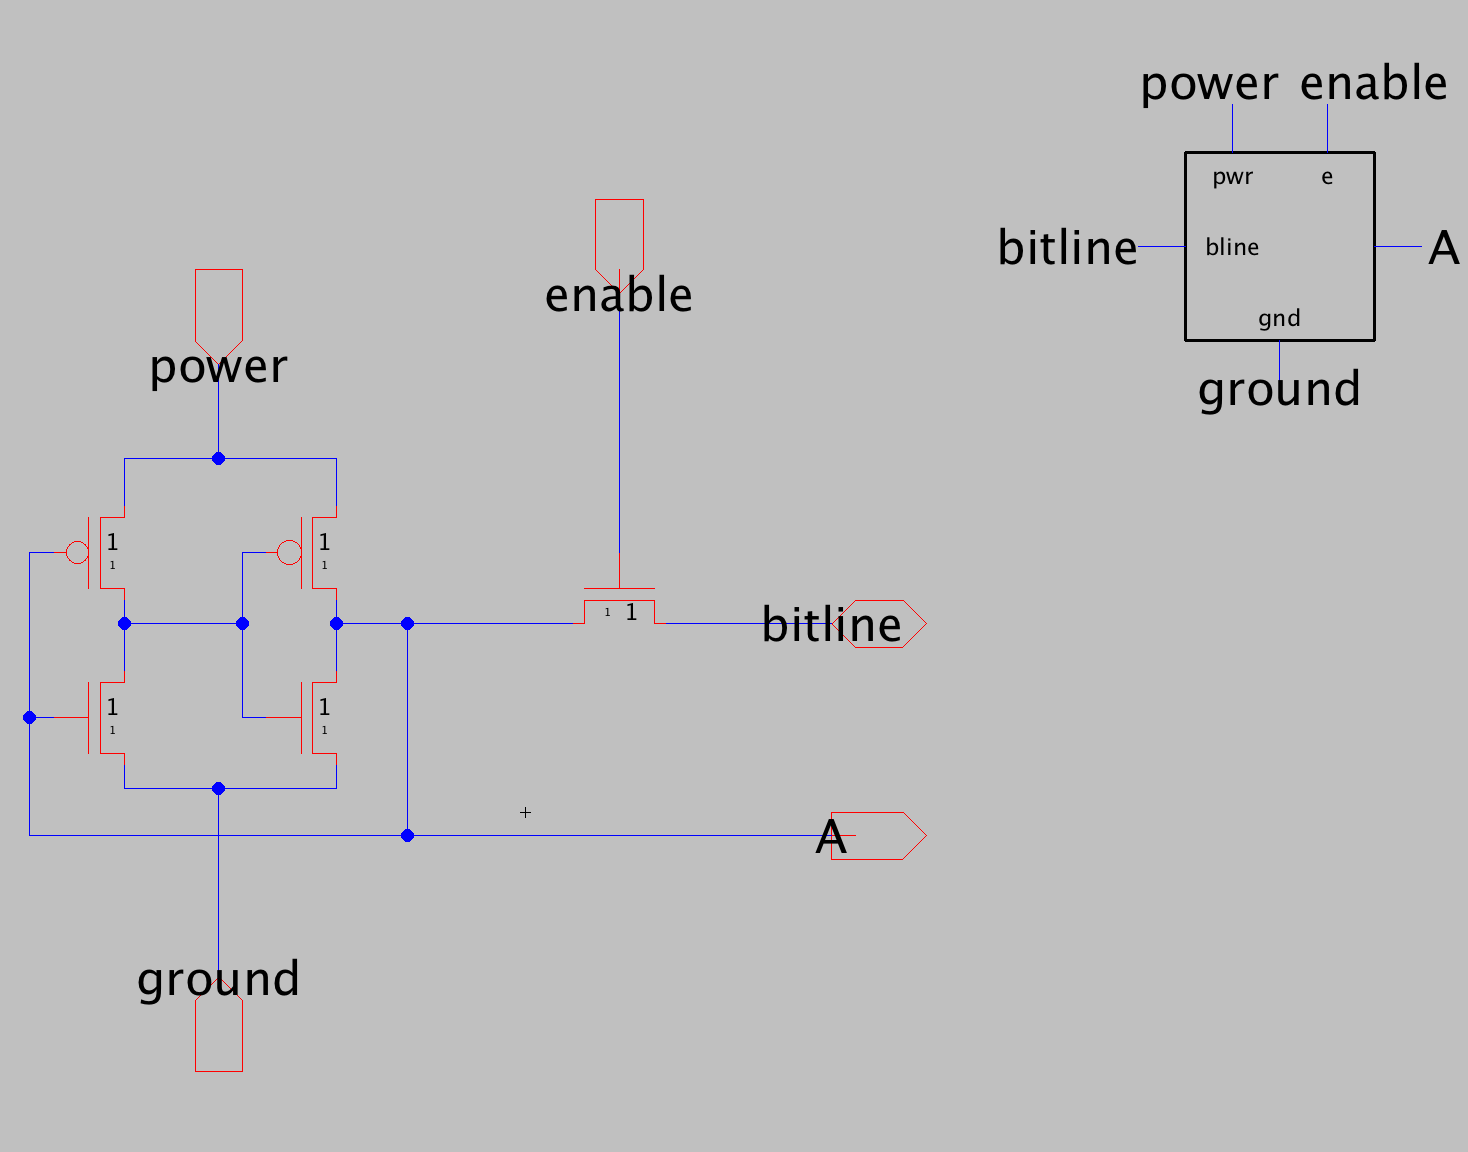
\includegraphics[scale=0.2]{5TCell}
 \caption{5T Memory Cell Schematic}
 \label{fig:5TCell}
\end{figure}
 
To check the correctness of our design, we performed multiple tests. We created a special version of our ultimate memory cell with an output of A so that we can see the fluctuations of the held value. Below is the setup for our test bench.\\

\begin{figure}[H]
	\centering
	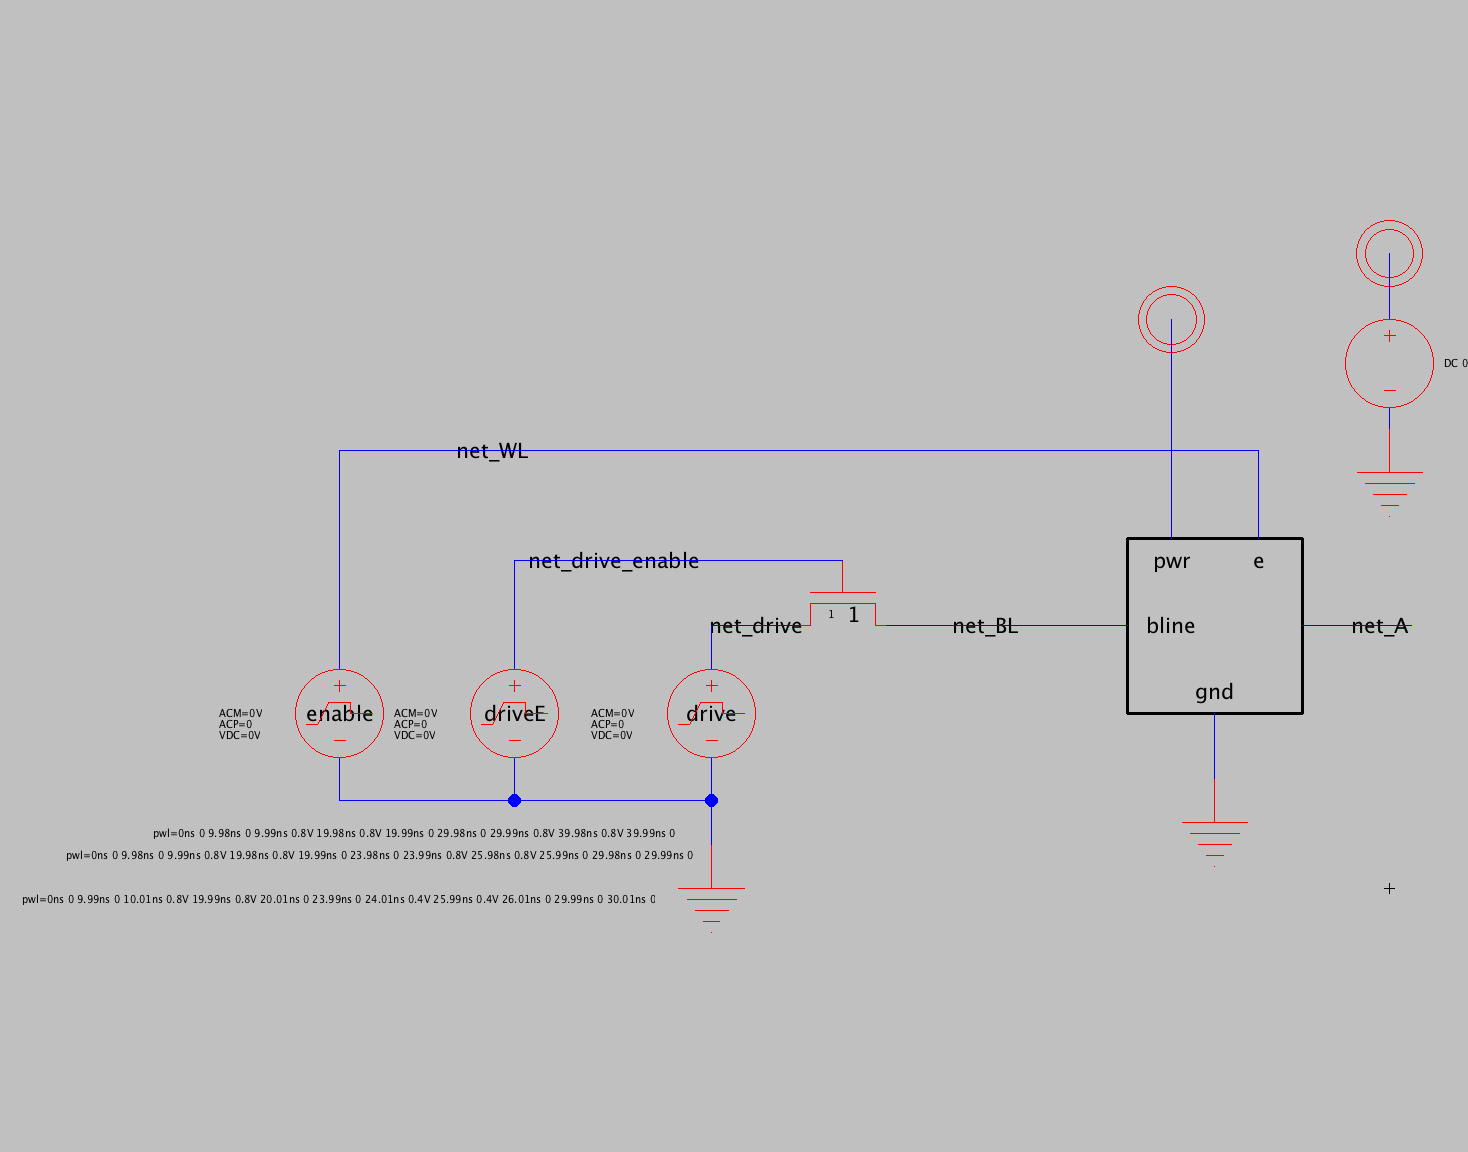
\includegraphics[scale=0.2]{5TCellTest}
	\caption{5TCell Test Schematic}
	\label{fig:5TCellTest}
\end{figure}

 To start, we wrote a 1 to the memory cell and then read from the same cell. Below is the output waveform of that test.\\
 
 \begin{figure}[H]
	\centering
	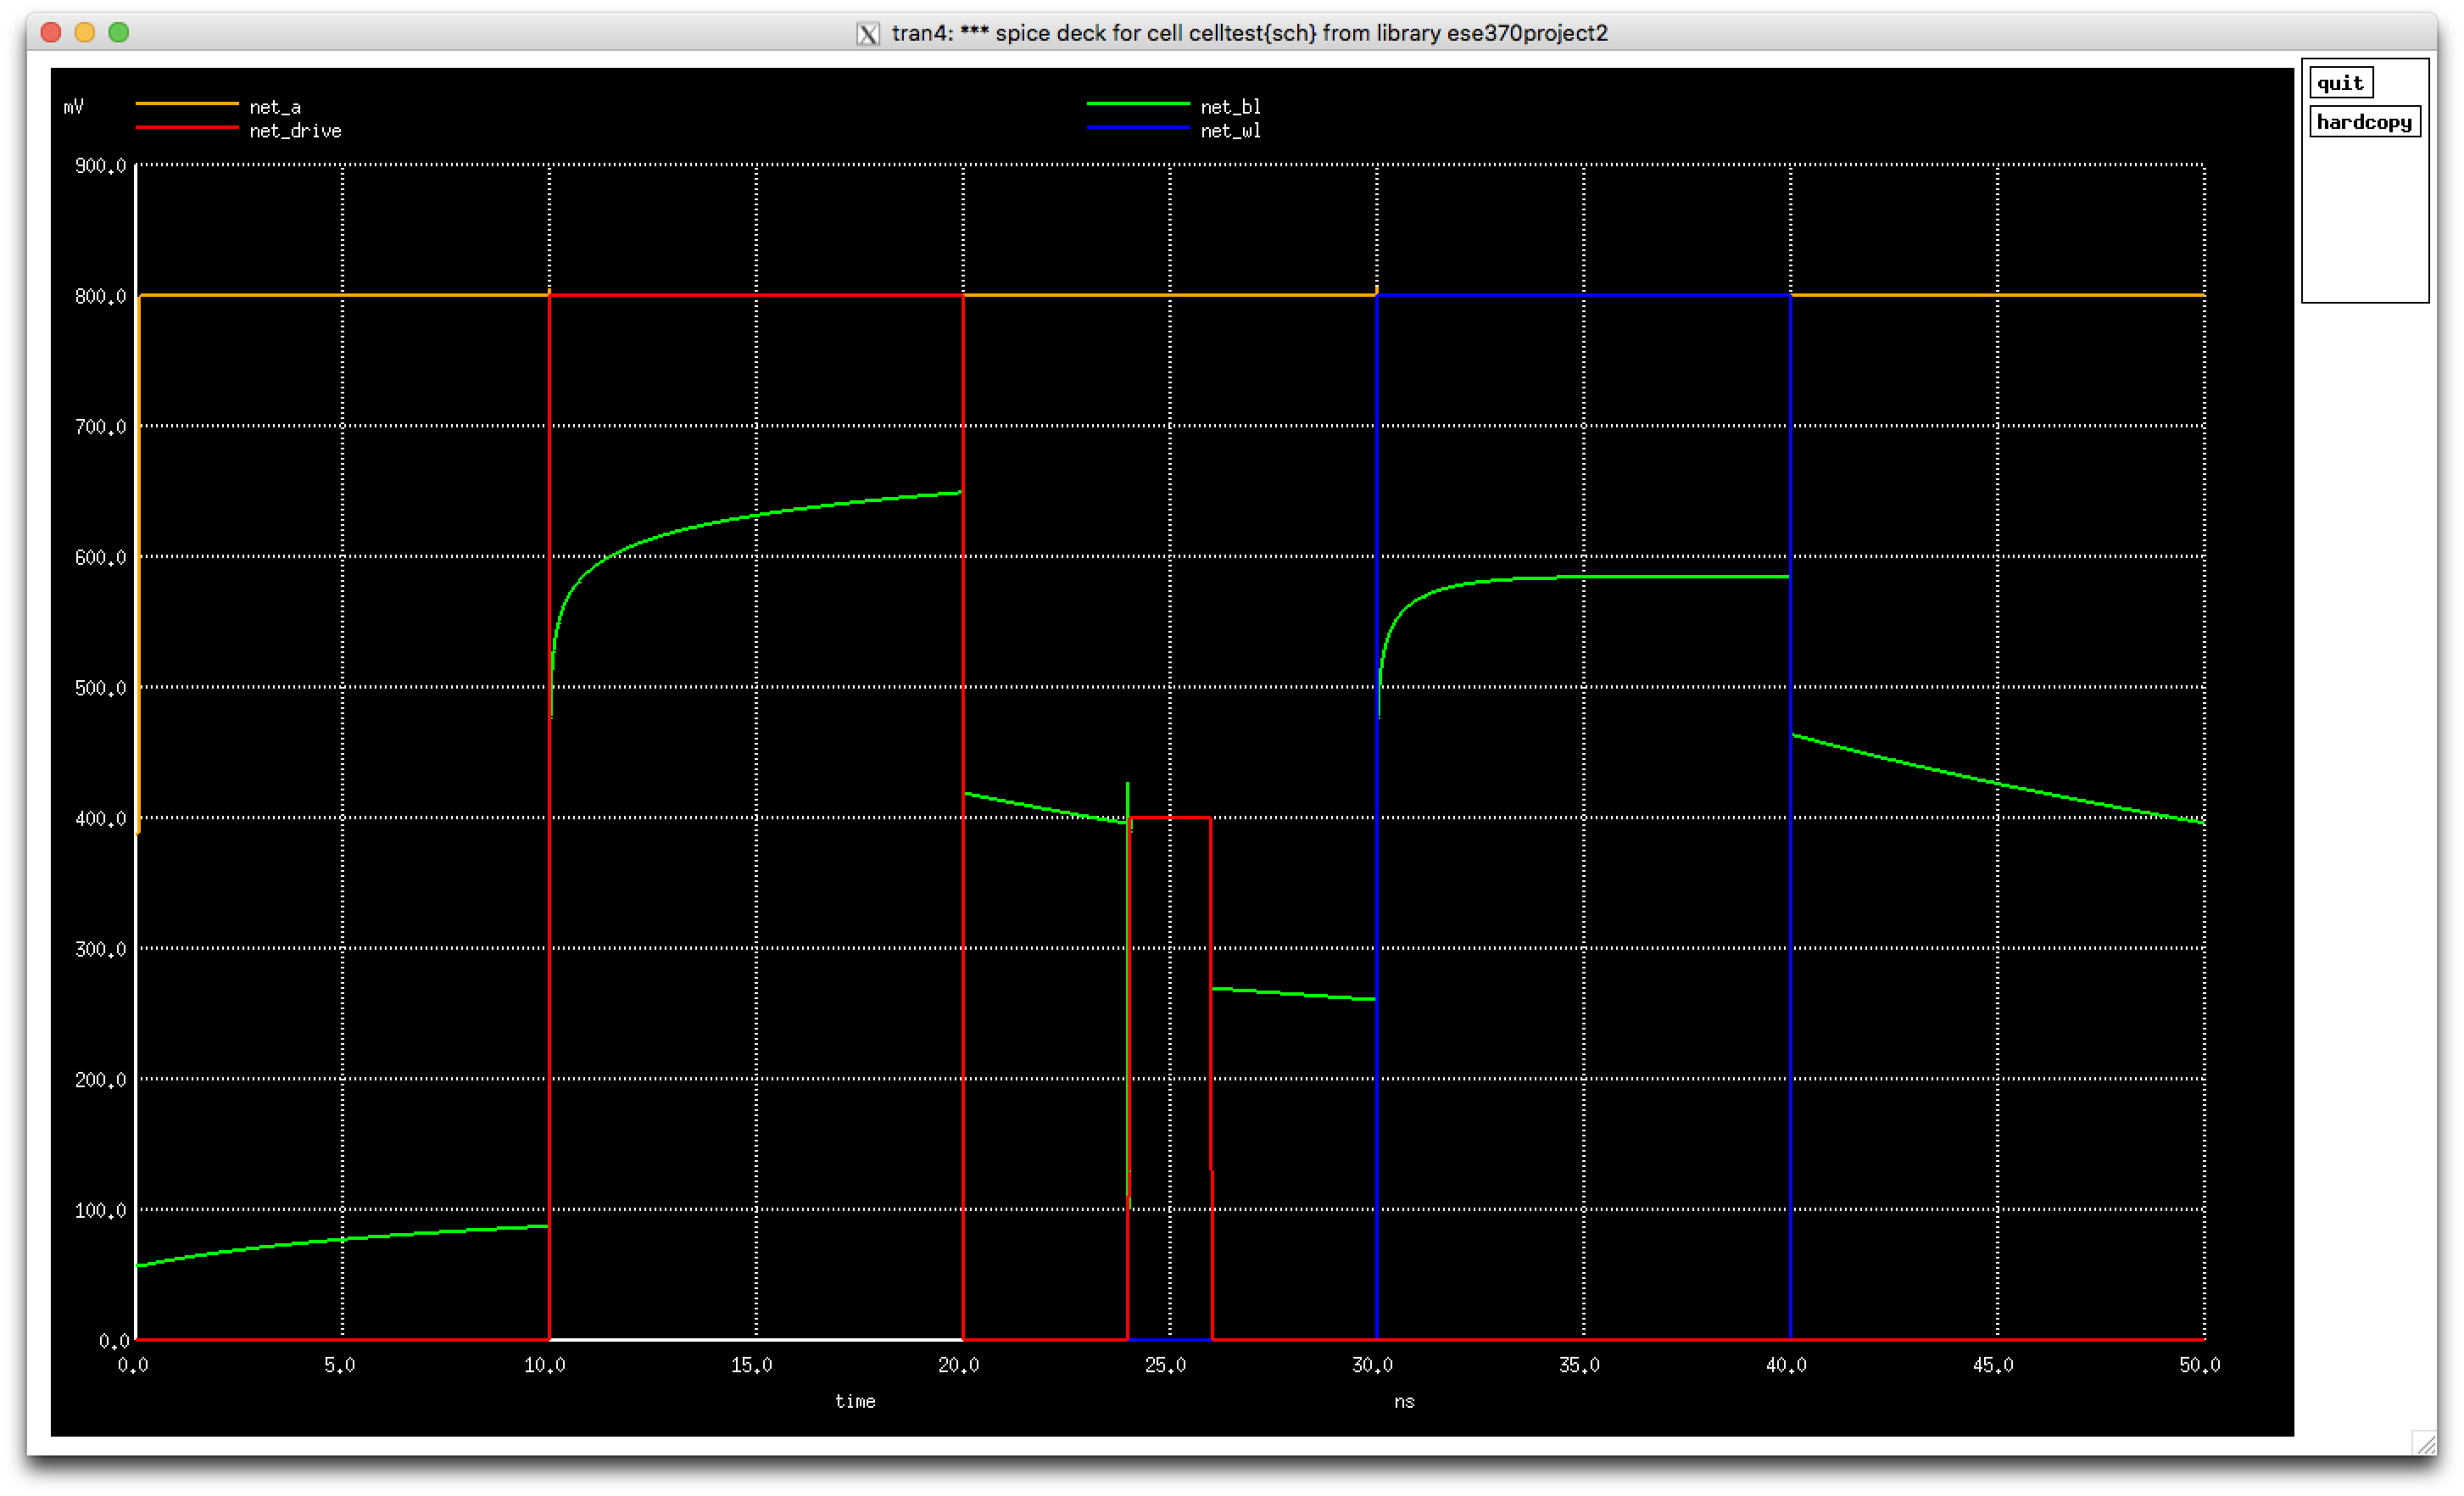
\includegraphics[scale=0.12]{5TWR1}
	\caption{5TCell Write/Read 1}
	\label{fig:5TWR1}
\end{figure}
We zoomed in on the point where \textbf{A} is written to a 1 which is shown below.\\

 \begin{figure}[H]
	\centering
	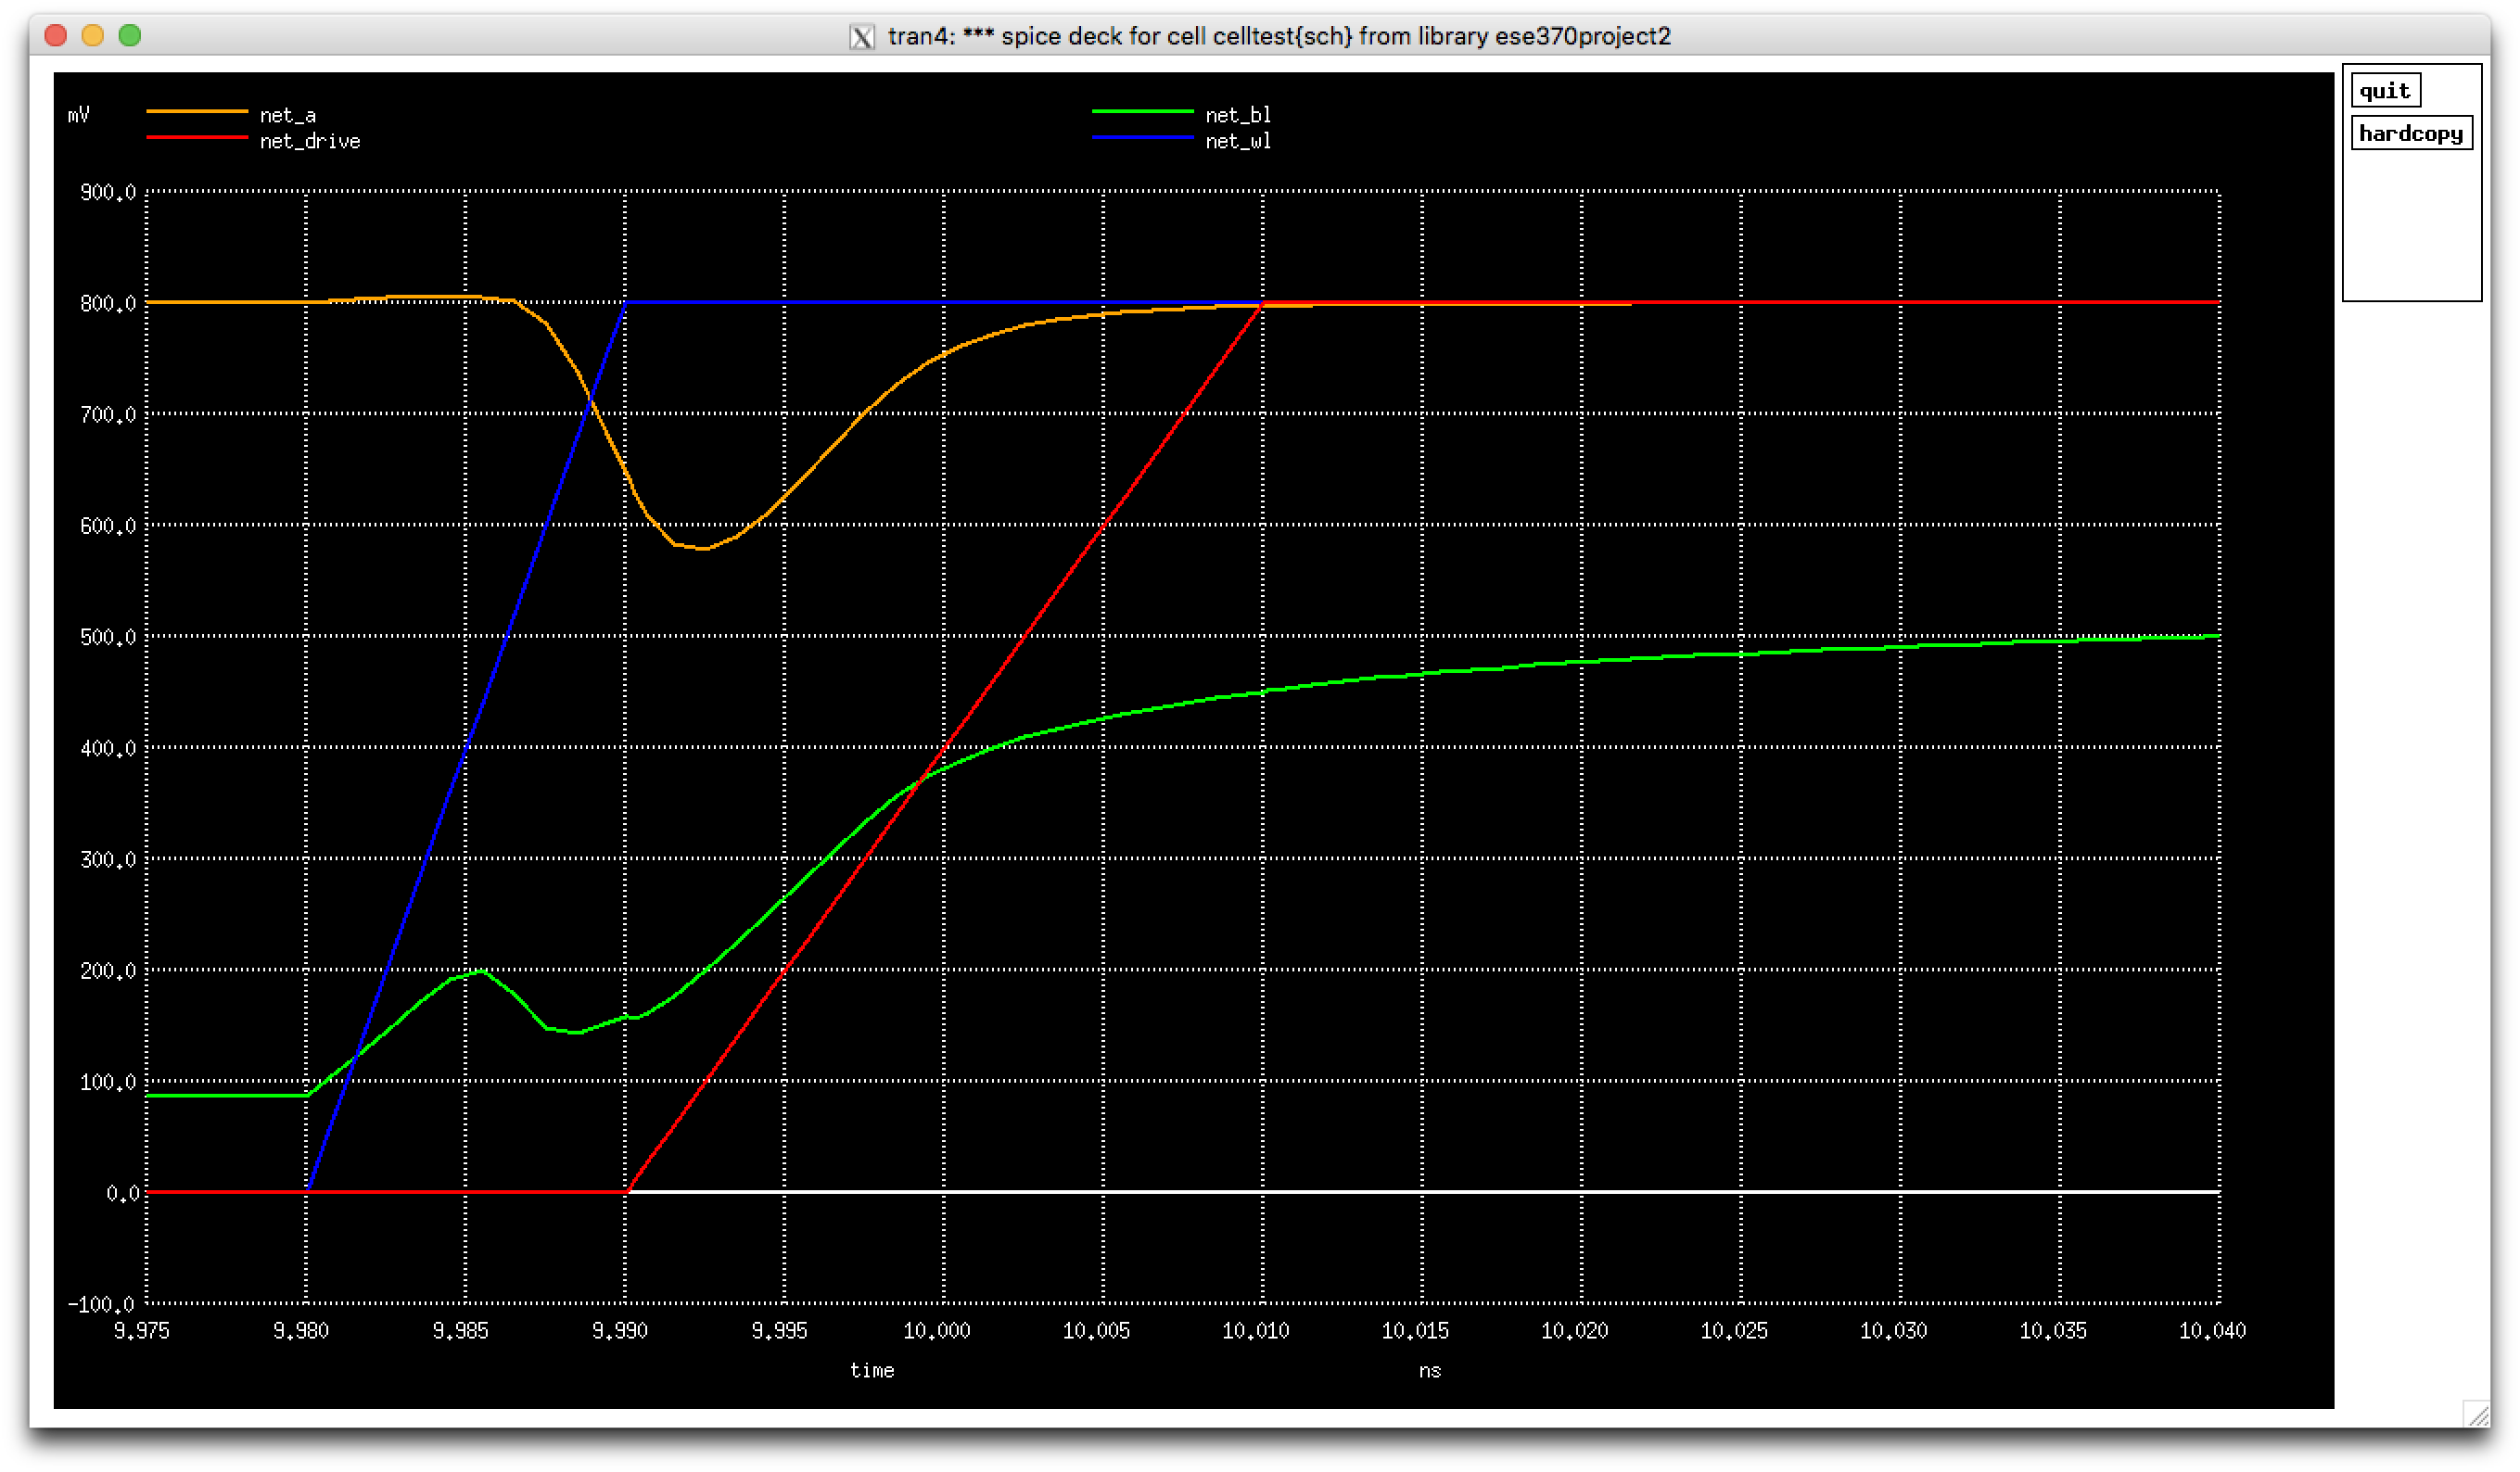
\includegraphics[scale=0.12]{5TWrite1}
	\caption{5TCell Write 1}
	\label{fig:5TWrite1}
\end{figure}

Here you can see the slight dip in \textbf{A} before the drive line goes high. As the driving signal goes high, \textbf{A} responds accordingly. We also checked the zoomed part of the read operation (Figure \ref{fig:5TRead1}).

 \begin{figure}[H]
	\centering
	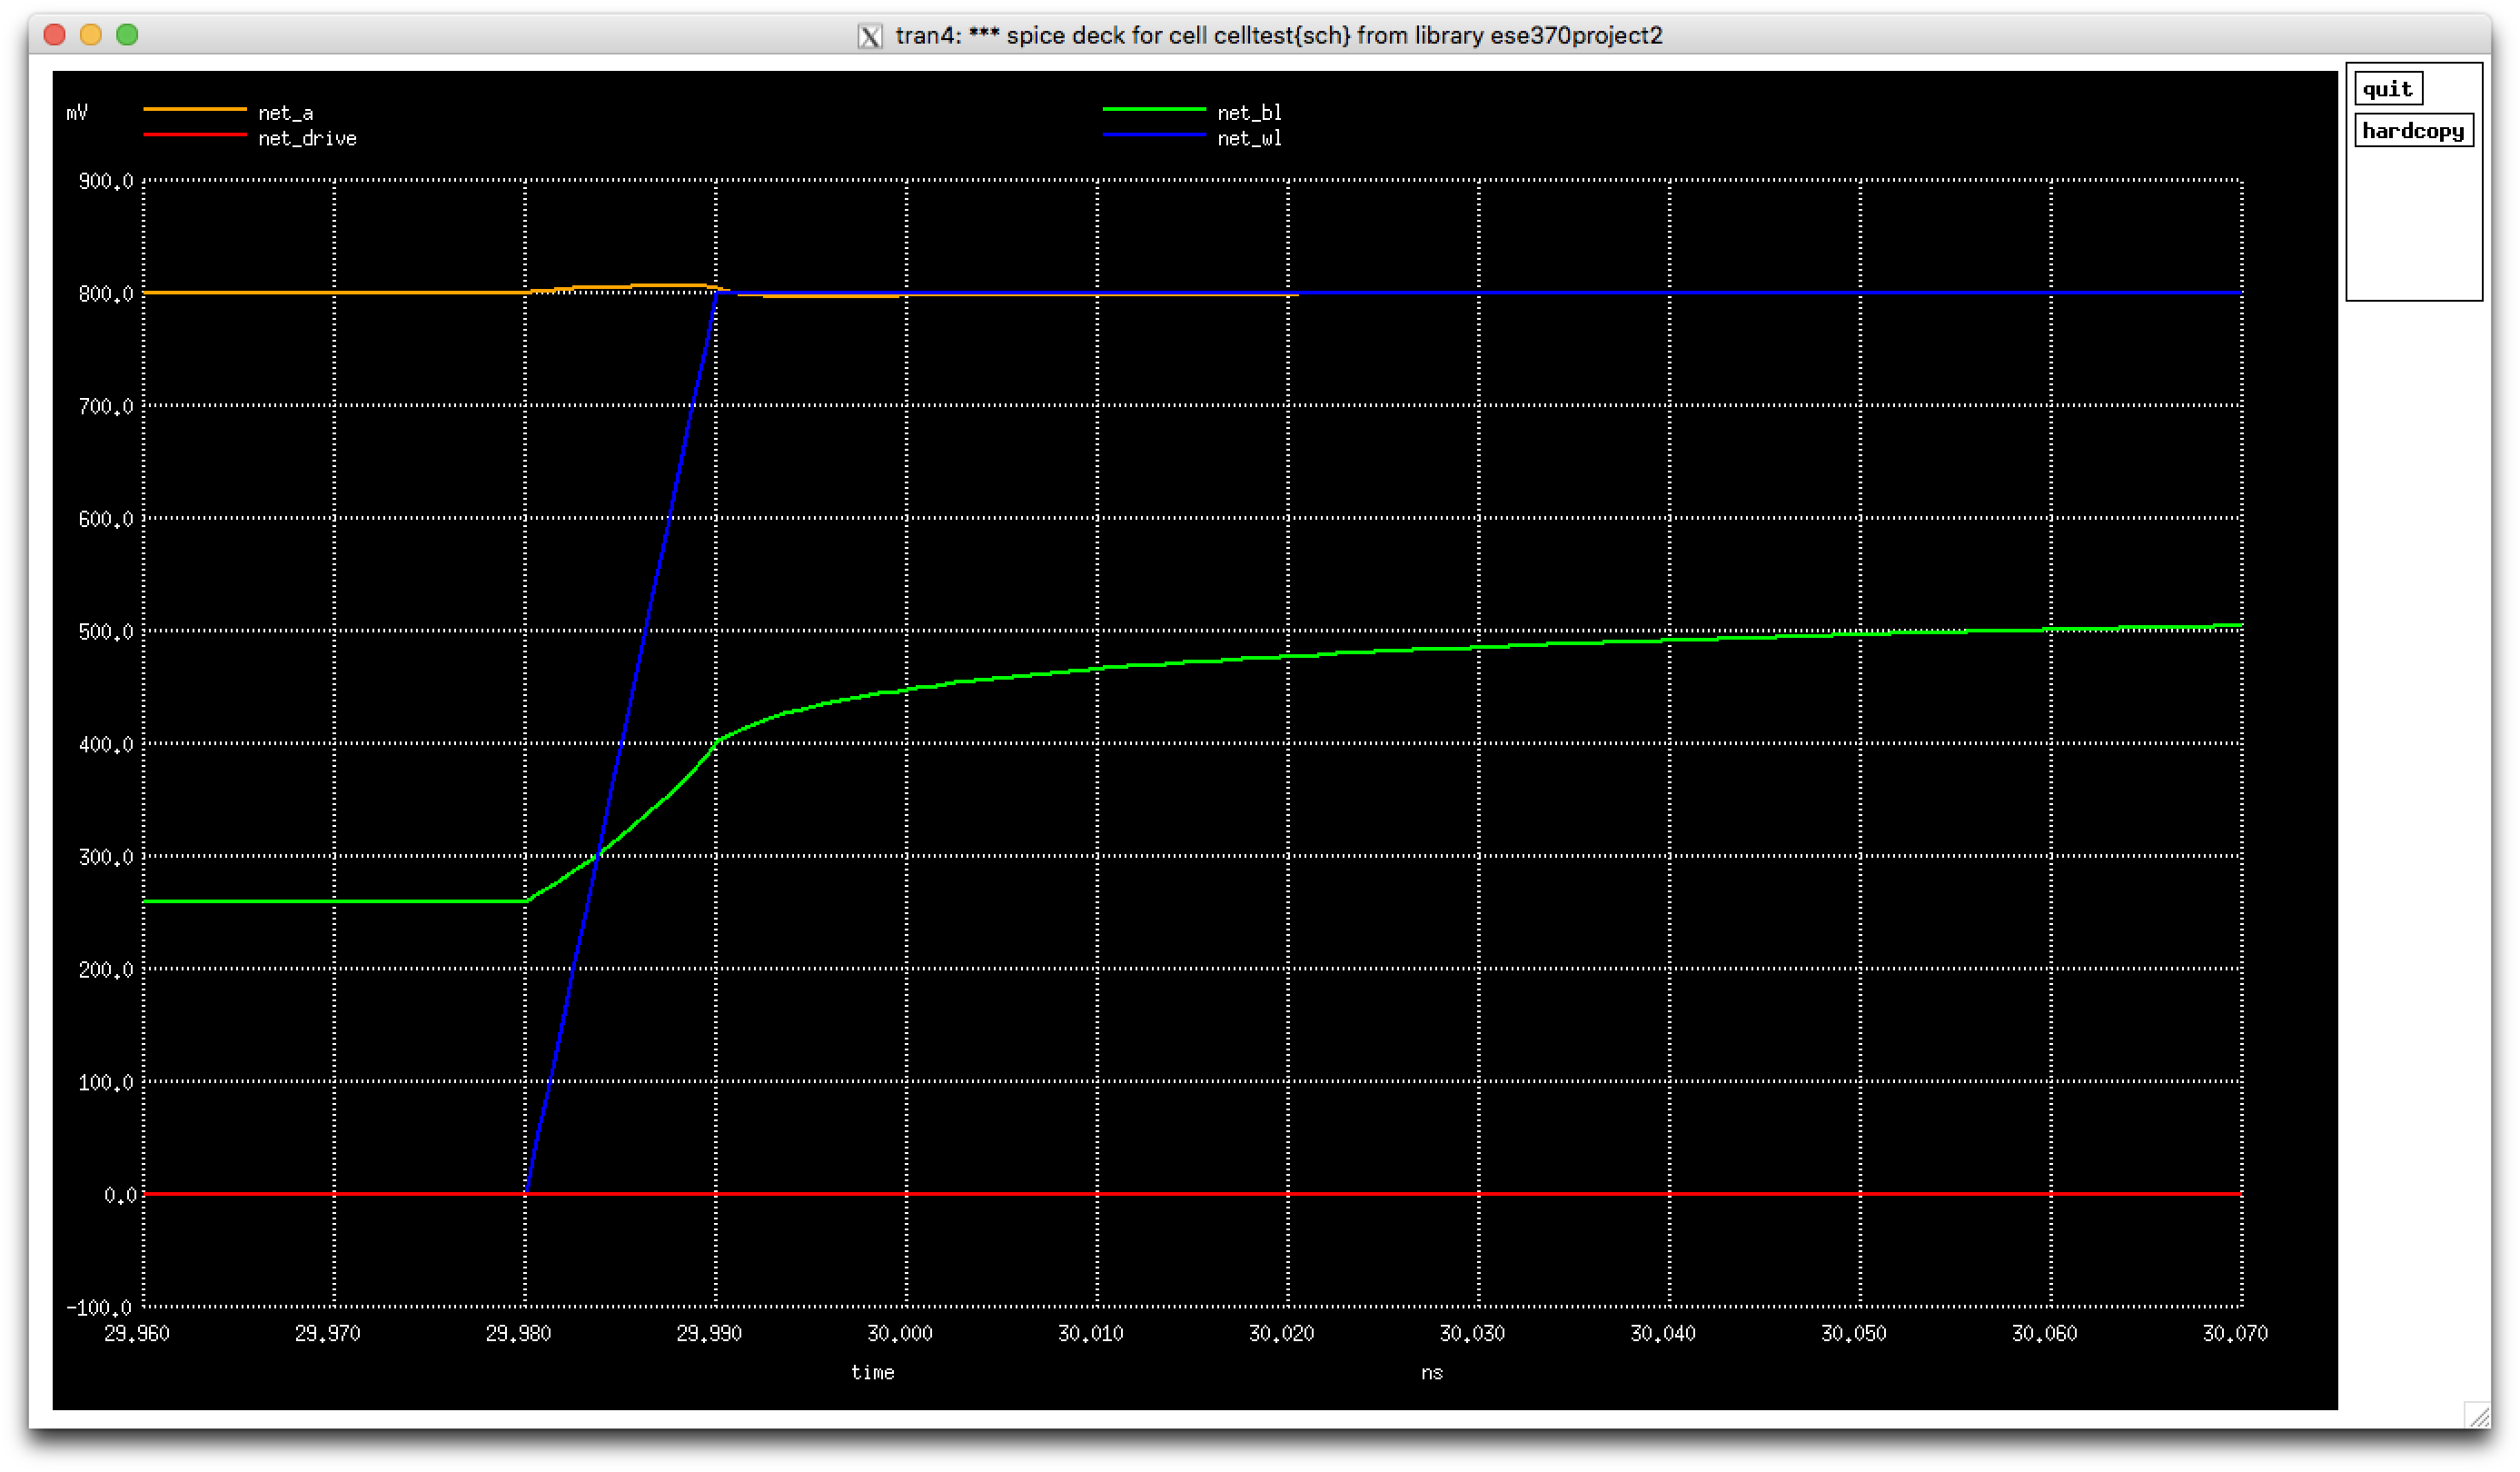
\includegraphics[scale=0.12]{5TRead1}
	\caption{5TCell Read 1}
	\label{fig:5TRead1}
\end{figure}

To validate correctness of our memory cell, we also checked performing back-to-back read operations after a write. Below is our test to verify that A did was not overwritten by a read in case \textbf{A} = 1.

 \begin{figure}[H]
	\centering
	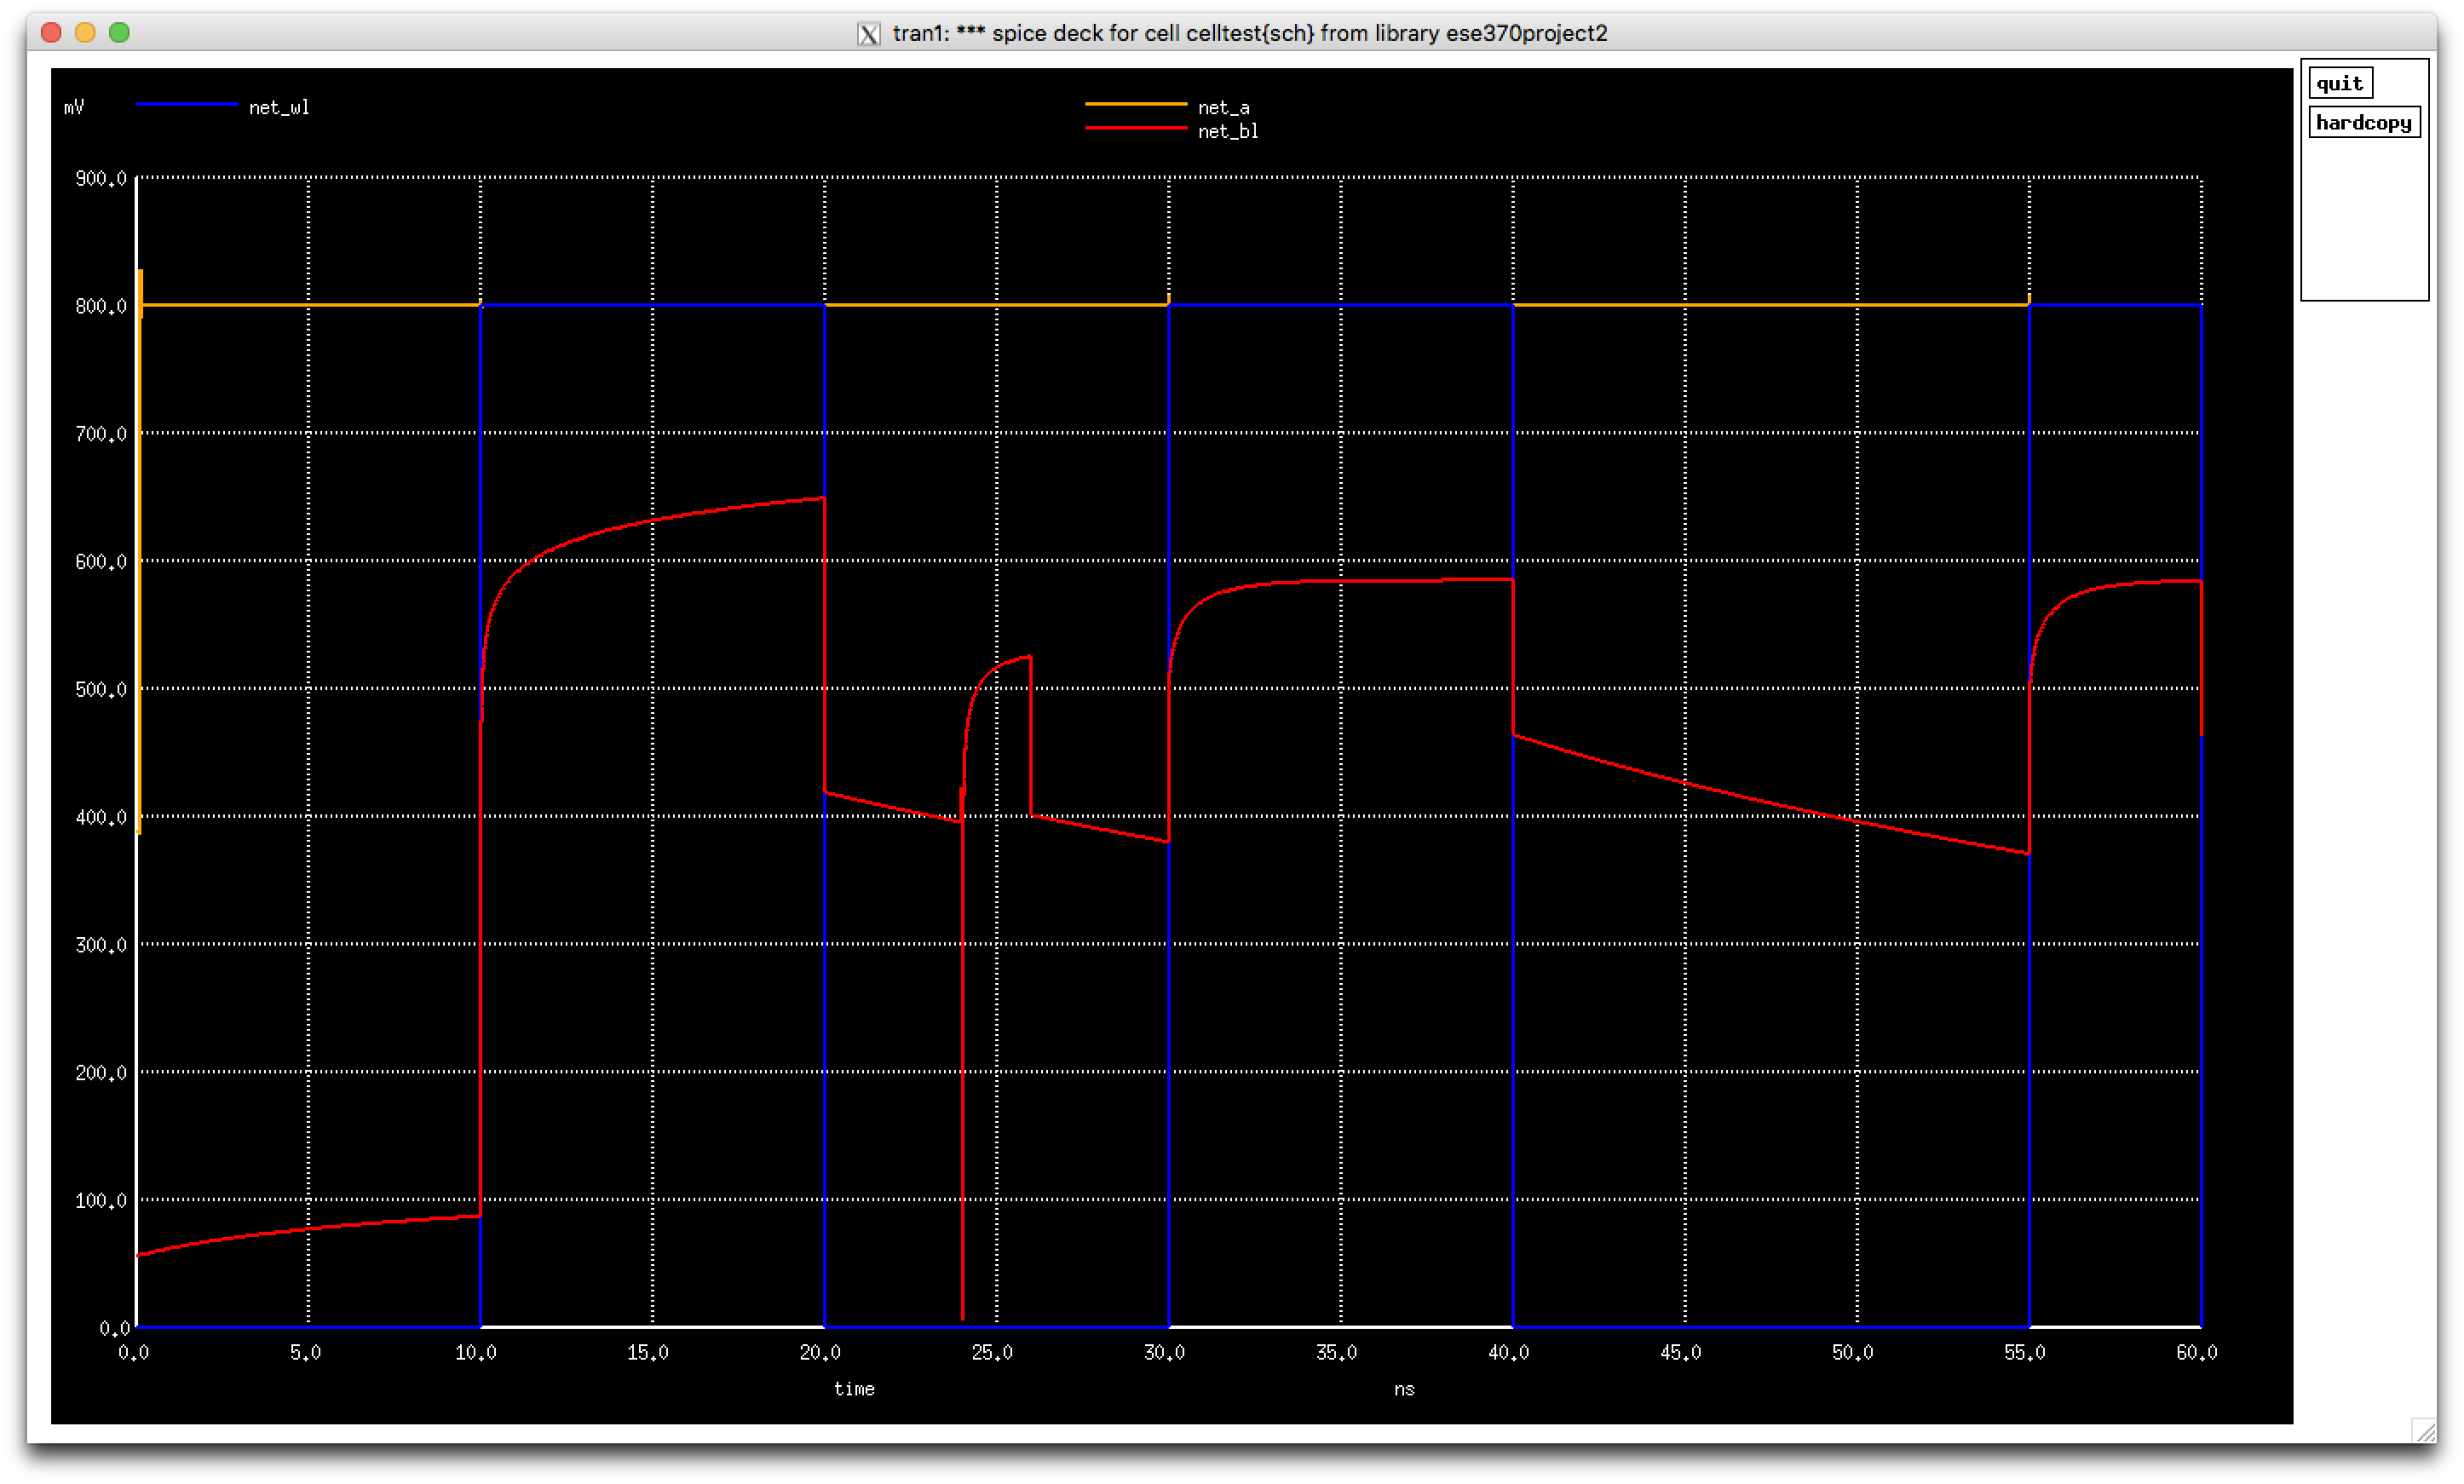
\includegraphics[scale=0.12]{5TDoubleRead1}
	\caption{5TCell Back-to-Back Read 1}
	\label{fig:5TBackToBack1}
\end{figure}

We also checked the back-to-back read operation when \textbf{A} = 0.

 \begin{figure}[H]
	\centering
	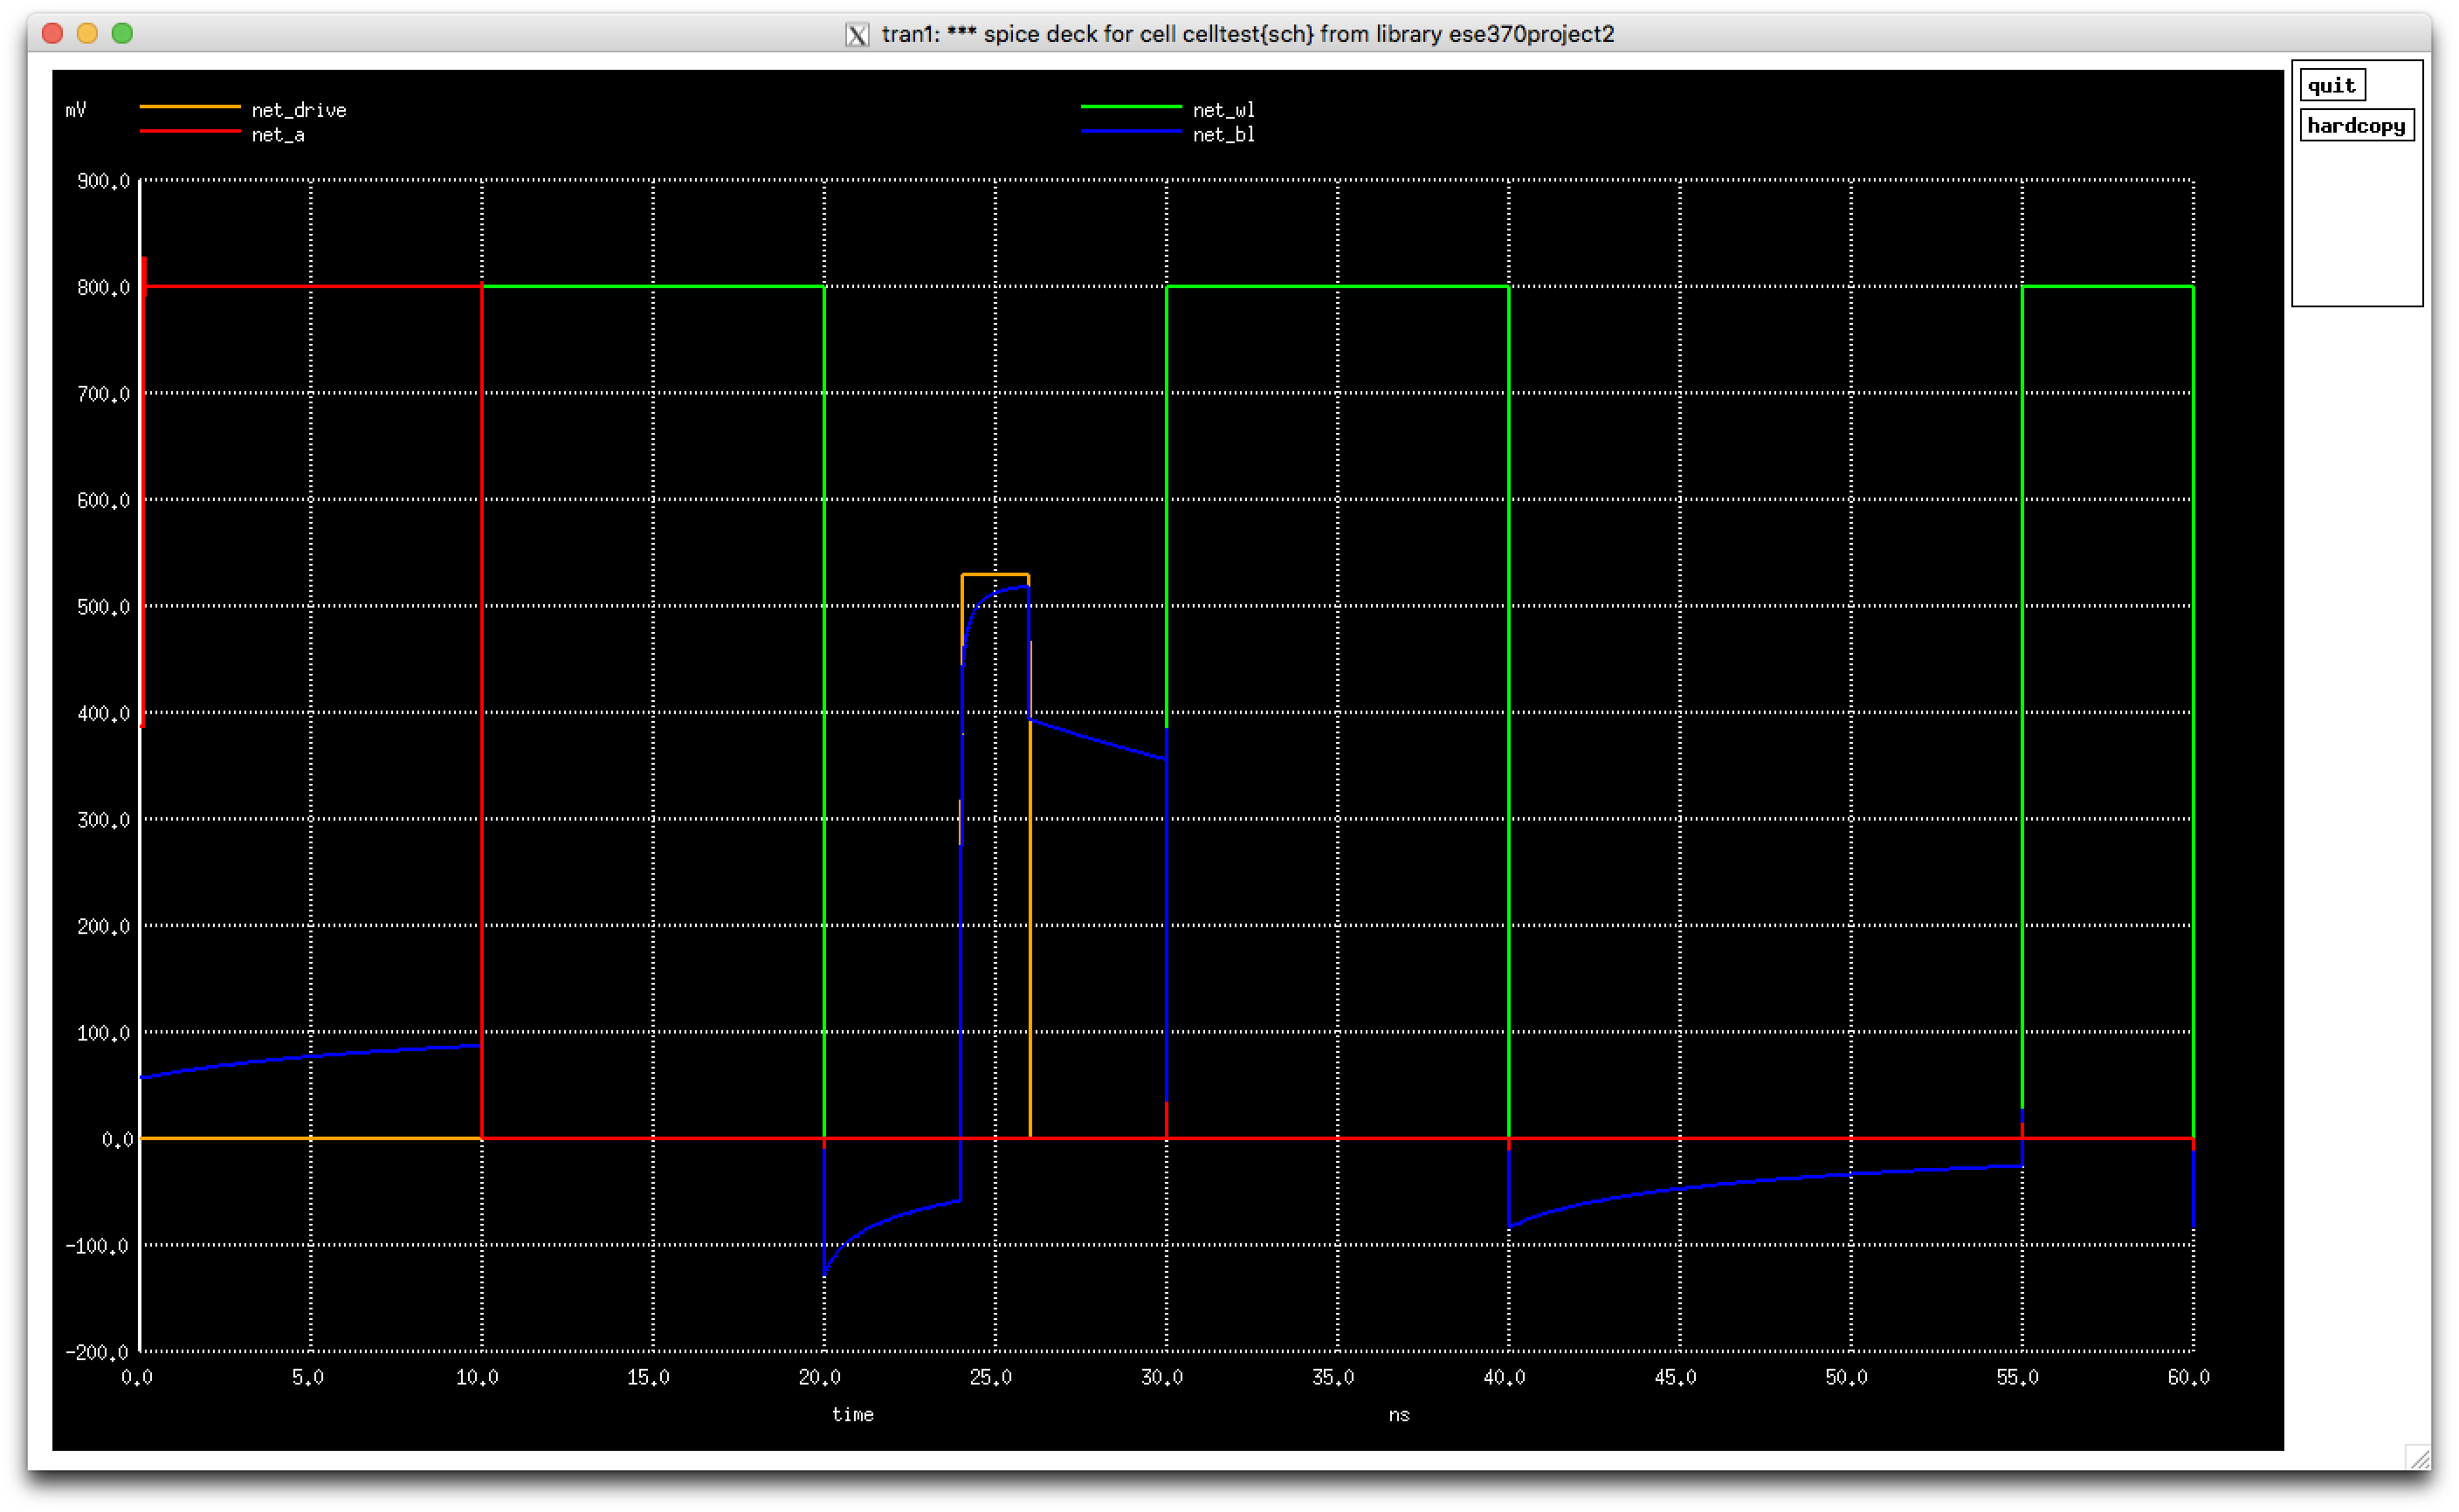
\includegraphics[scale=0.12]{5TDoubleRead0}
	\caption{5TCell Back-to-Back Read 0}
	\label{fig:5TBackToBack0}
\end{figure}

As the figure shows, \textbf{A} stays stable at 0.

\subsubsection{Sense Amplifier}
\label{sec:sense_amplifier}
We created a sense amplifier to try and help quicken the voltage pull up or down on the memory read. Below is the circuit for the sense amplifier.

\begin{figure}[H]
	\centering
	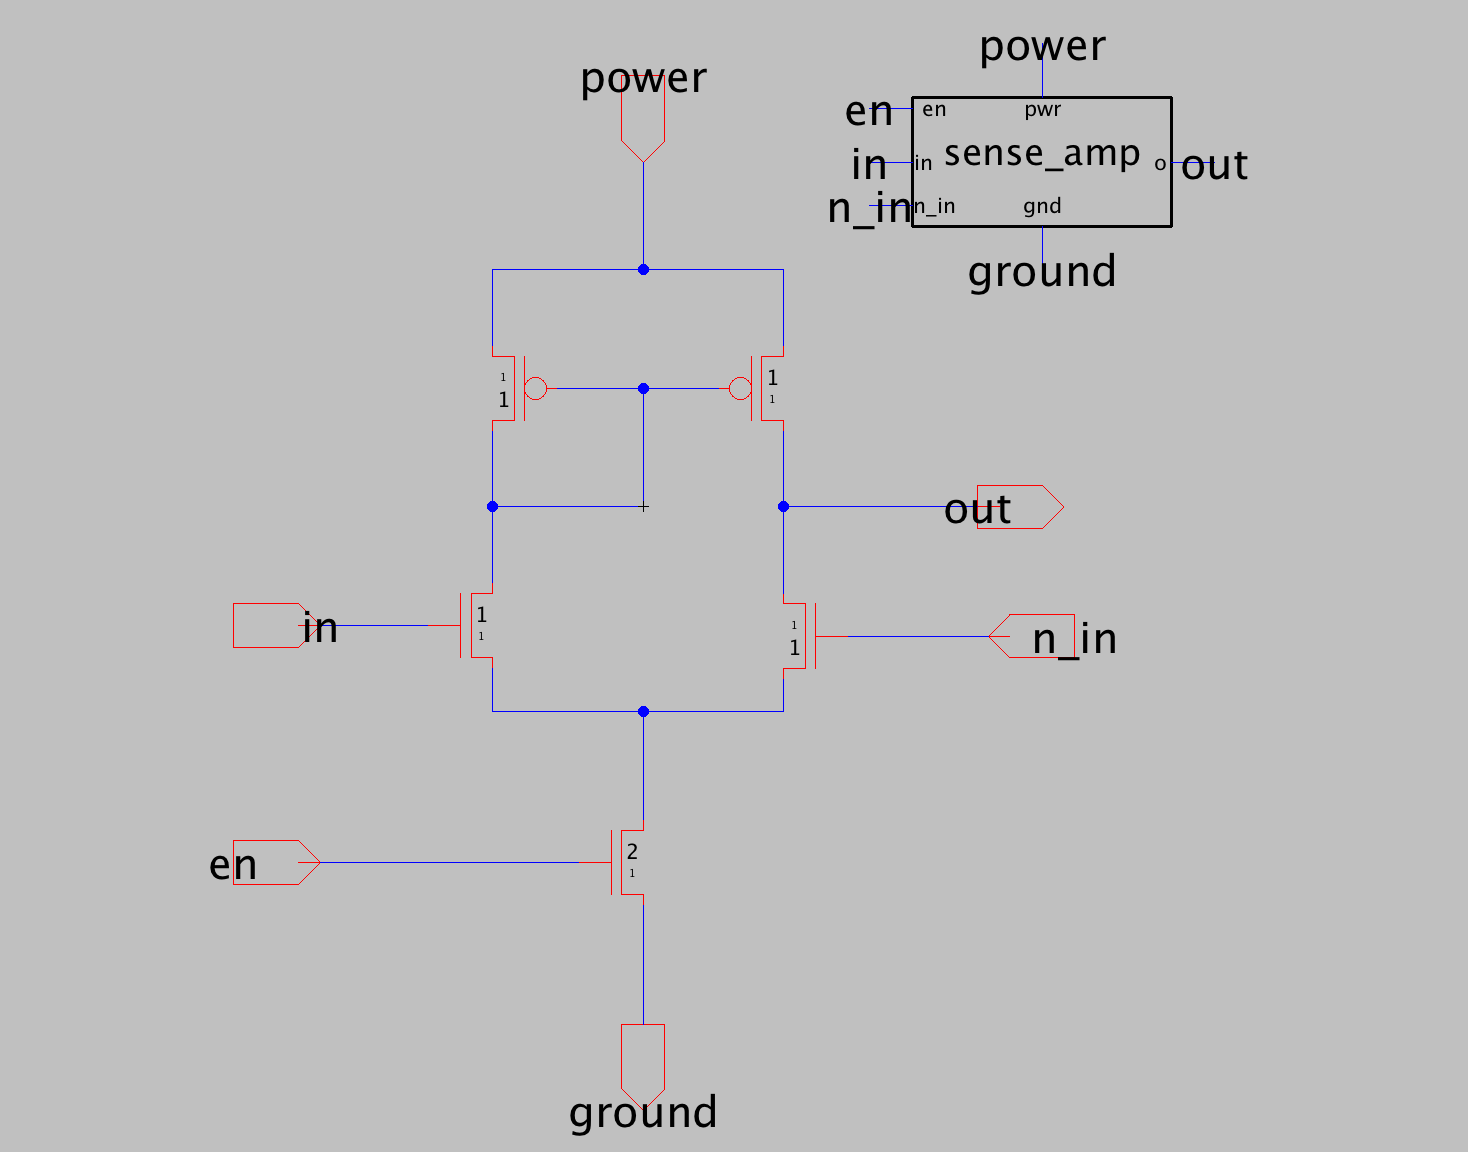
\includegraphics[scale=0.17]{senseAmp}
	\caption{Sense Amplifier}
	\label{fig:senseAmp}
\end{figure}

Below is the waveform for testing the sense amplifier.

\begin{figure}[H]
	\centering
	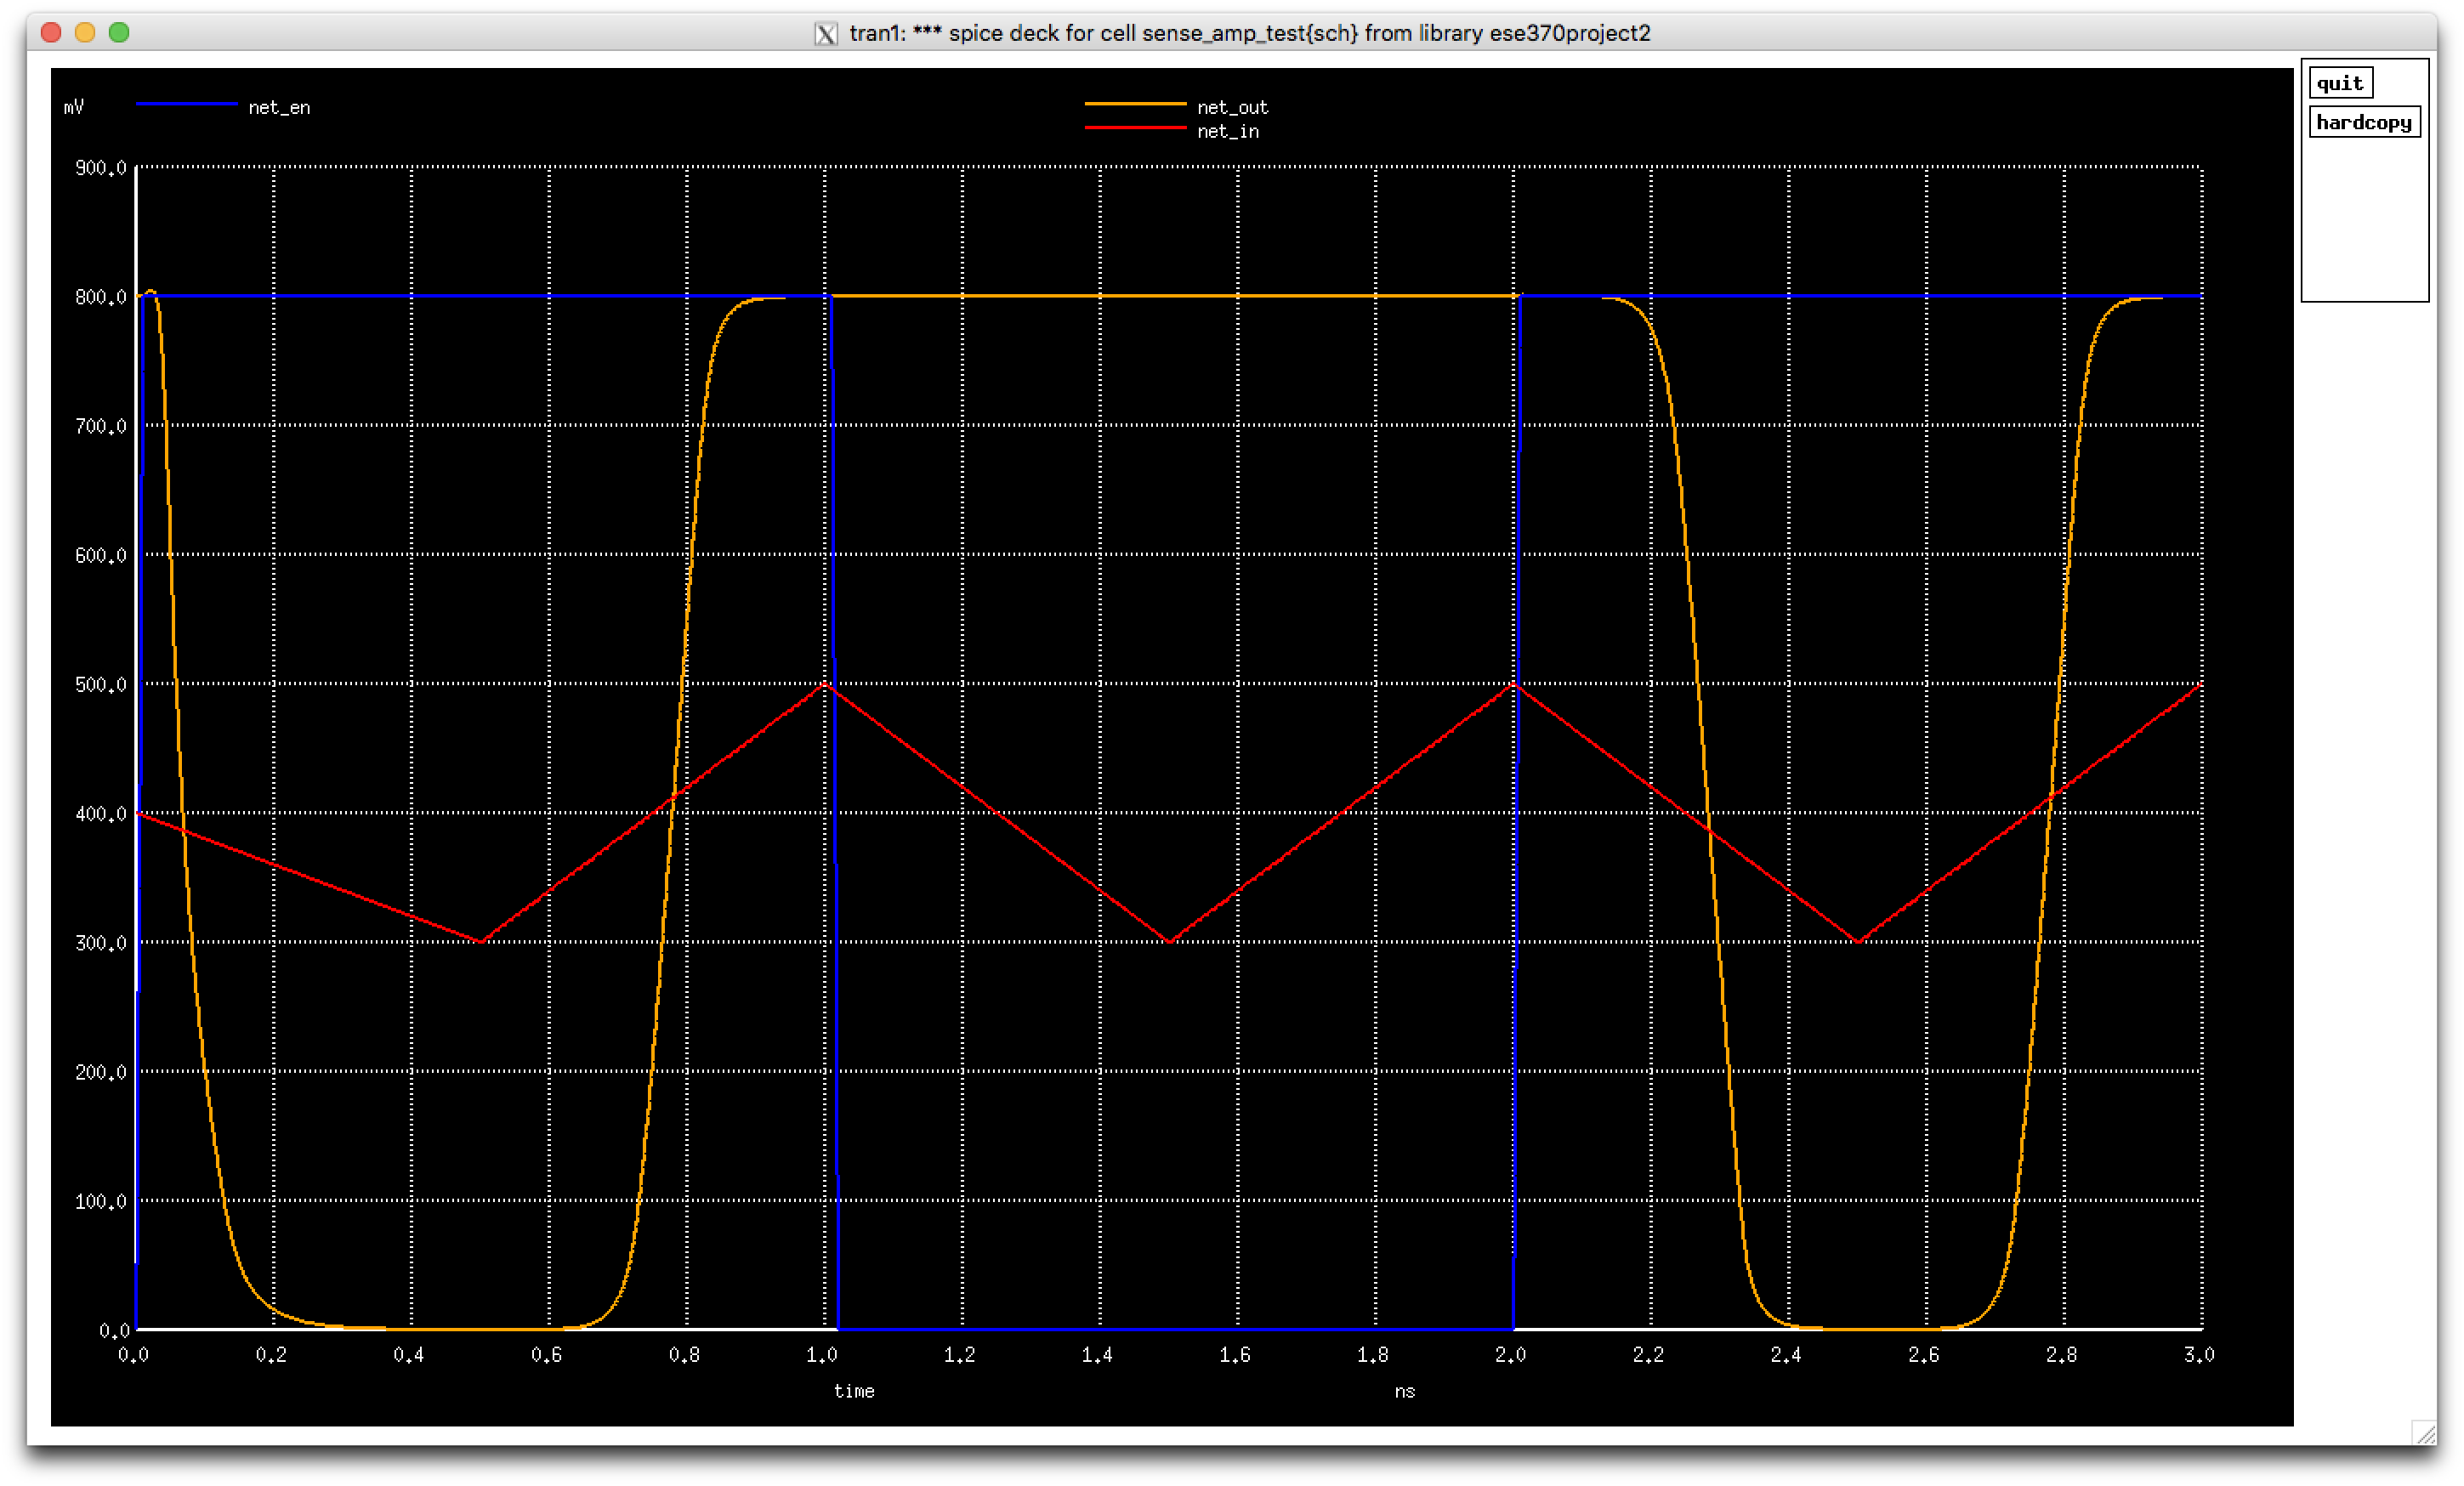
\includegraphics[scale=0.12]{senseAmpWave}
	\caption{Sense Amplifier Waveform}
	\label{fig:senseAmpWave}
\end{figure}

\subsubsection{$\frac{\textbf{Vdd}}{\textbf{2}}$ Reference Generator}
Below is the circuit for our voltage reference ($\frac{\textbf{Vdd}}{\textbf{2}}$) generator as given in the assignment prompt.

\begin{figure}[H]
	\centering
	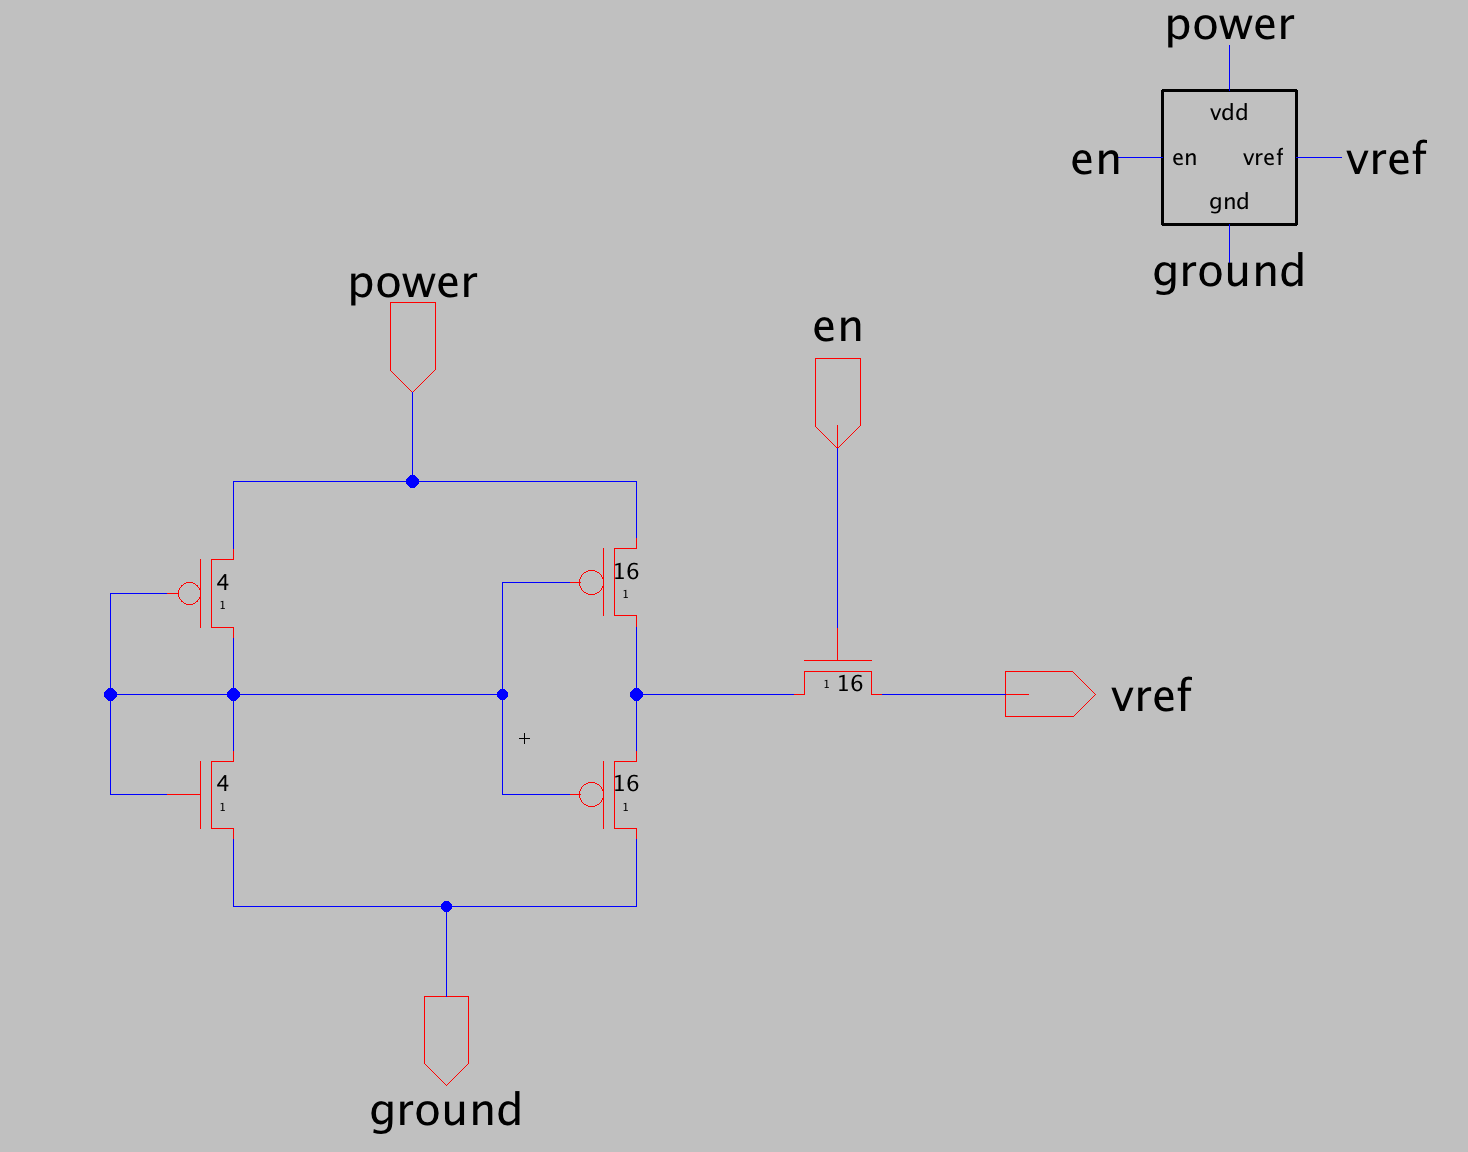
\includegraphics[scale=0.17]{vRefGen}
	\caption{Voltage Reference Generator}
	\label{fig:vRefGen}
\end{figure}

We tested the circuit with the below test bench.\\

\begin{figure}[H]
	\centering
	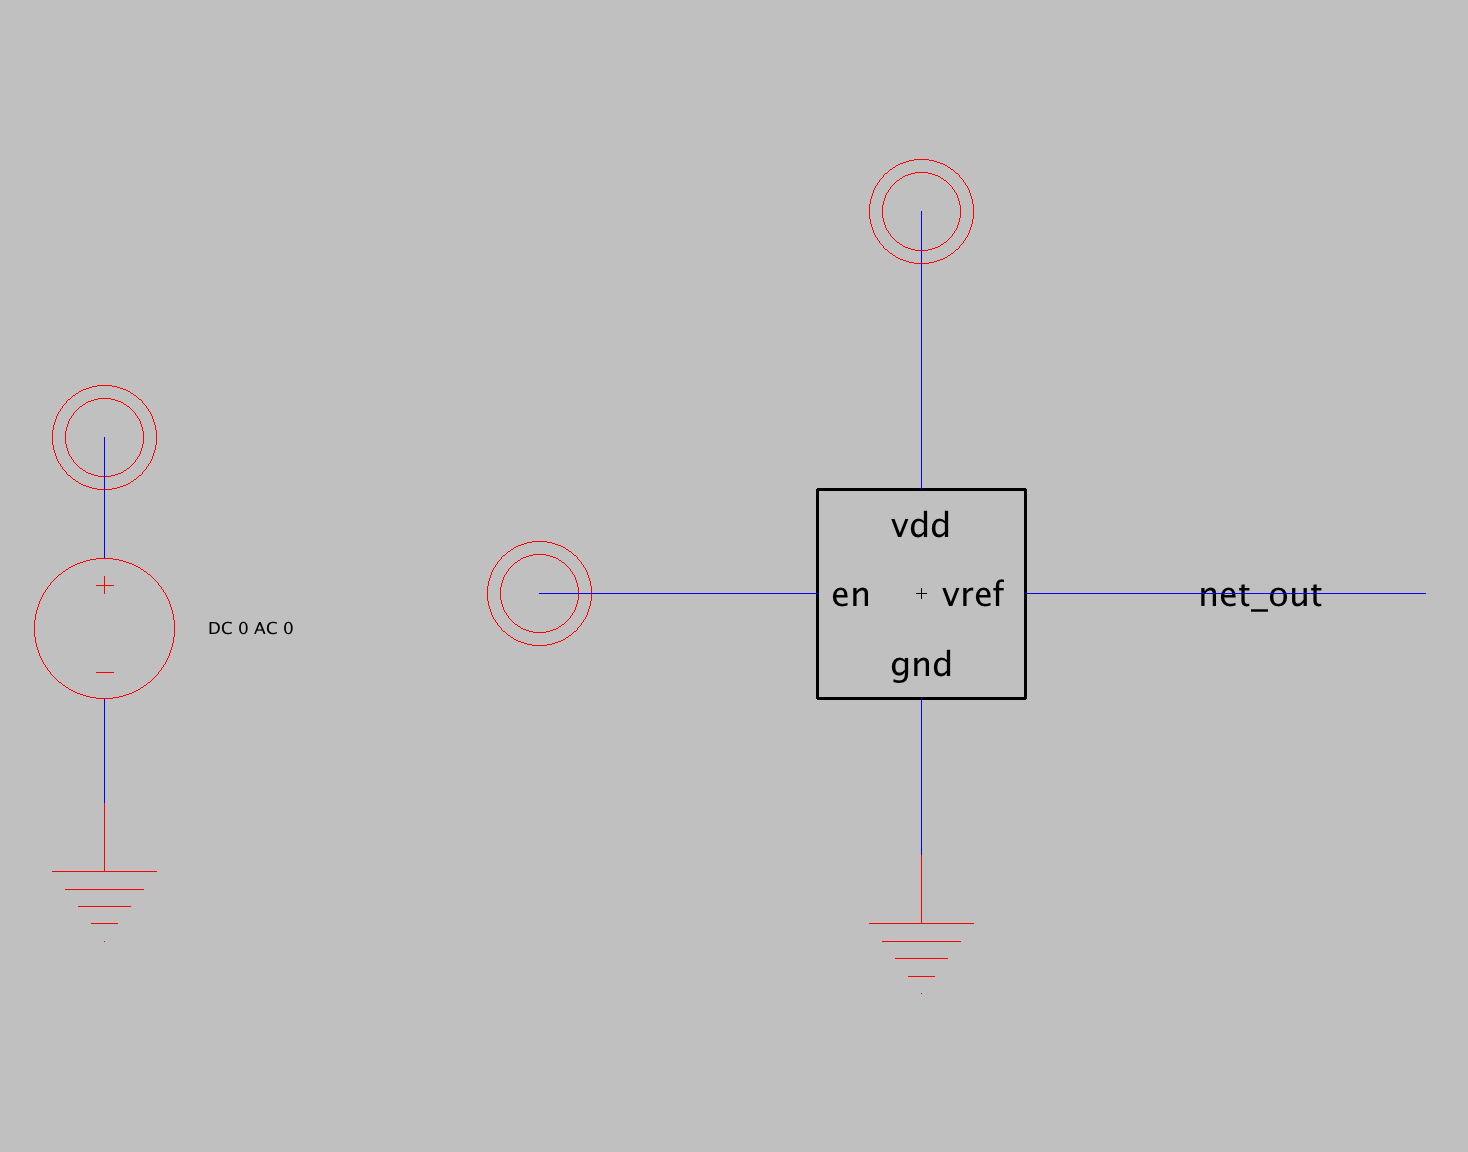
\includegraphics[scale=0.17]{vRefTest}
	\caption{Voltage Reference Generator Test Bench}
	\label{fig:vRefTest}
\end{figure}

With that test bench we generated the below waveform.\\

\begin{figure}[H]
	\centering
	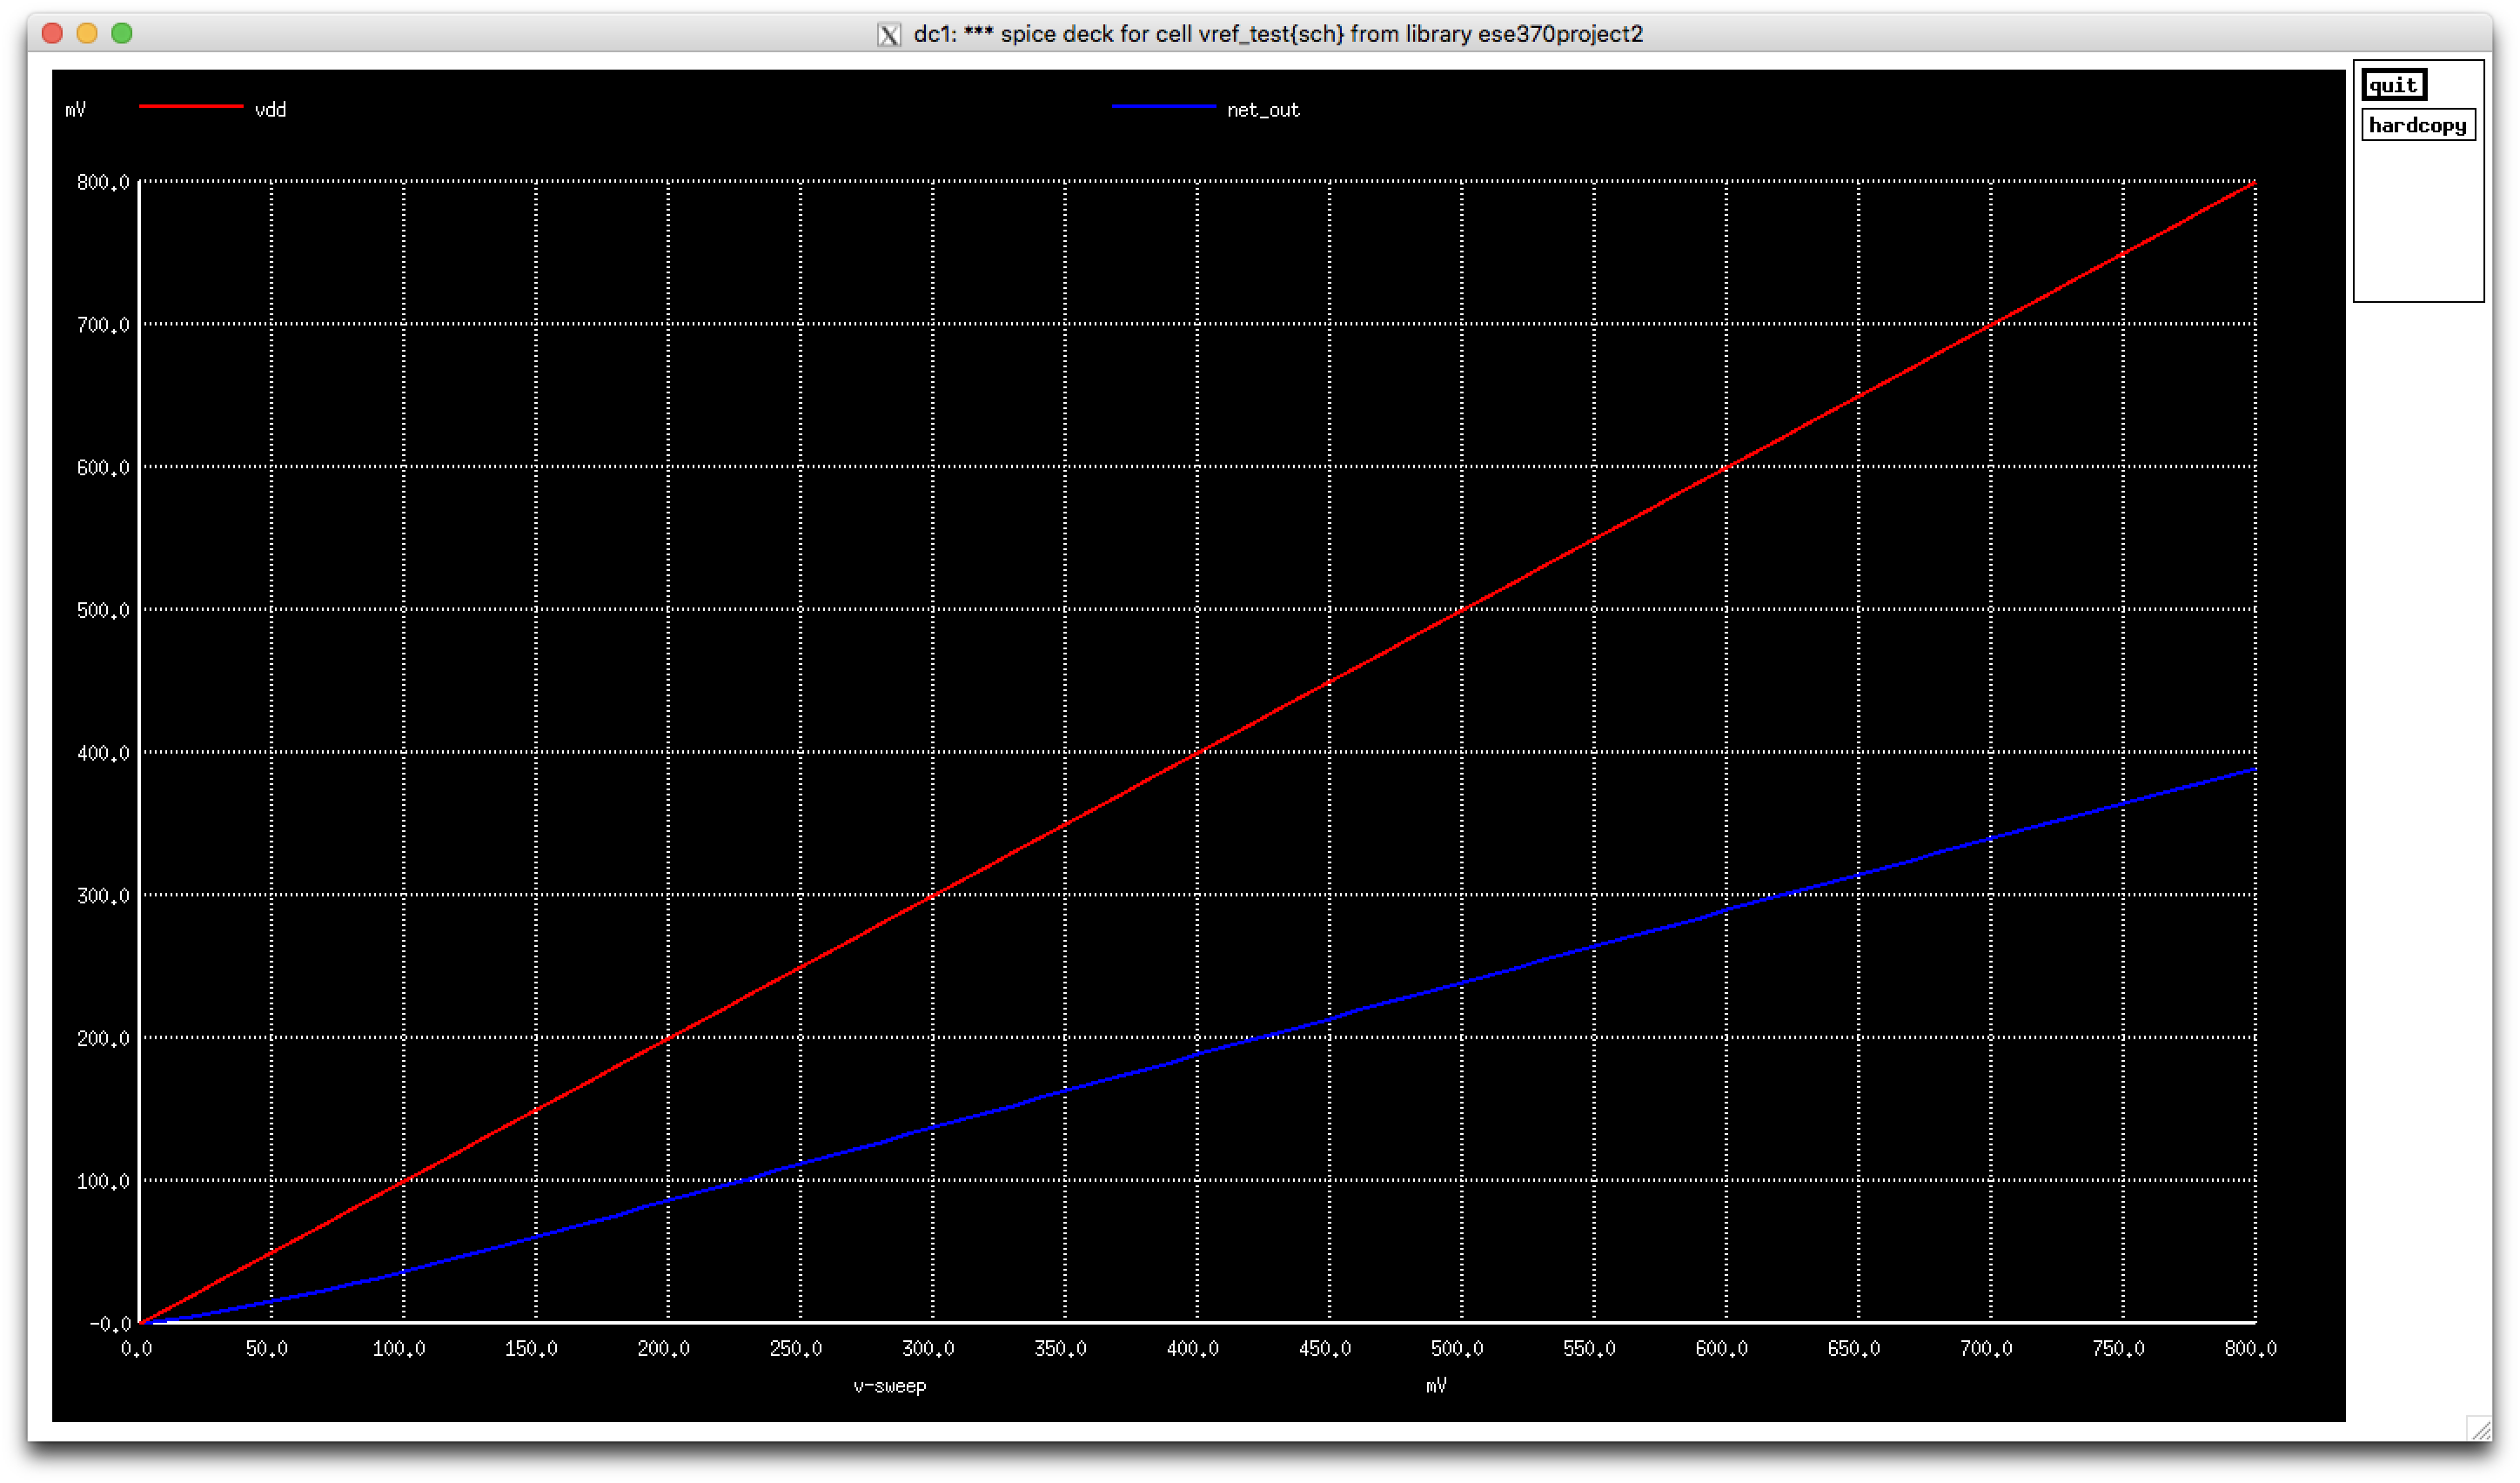
\includegraphics[scale=0.1]{vRefTestWave}
	\caption{Voltage Reference Generator Test Bench Waveform}
	\label{fig:vRefTestWave}
\end{figure}

You can see that for every given value of $V_{dd}$, the output is (or is very close to) half of $V_{dd}$.

\subsubsection{Bit Line Driver}

For the bitline driver we created a tri state buffer so that we could control when and how the bitline was driven. Below is the schematic for the circuit followed by our test bench.

\begin{figure}[H]
	\centering
	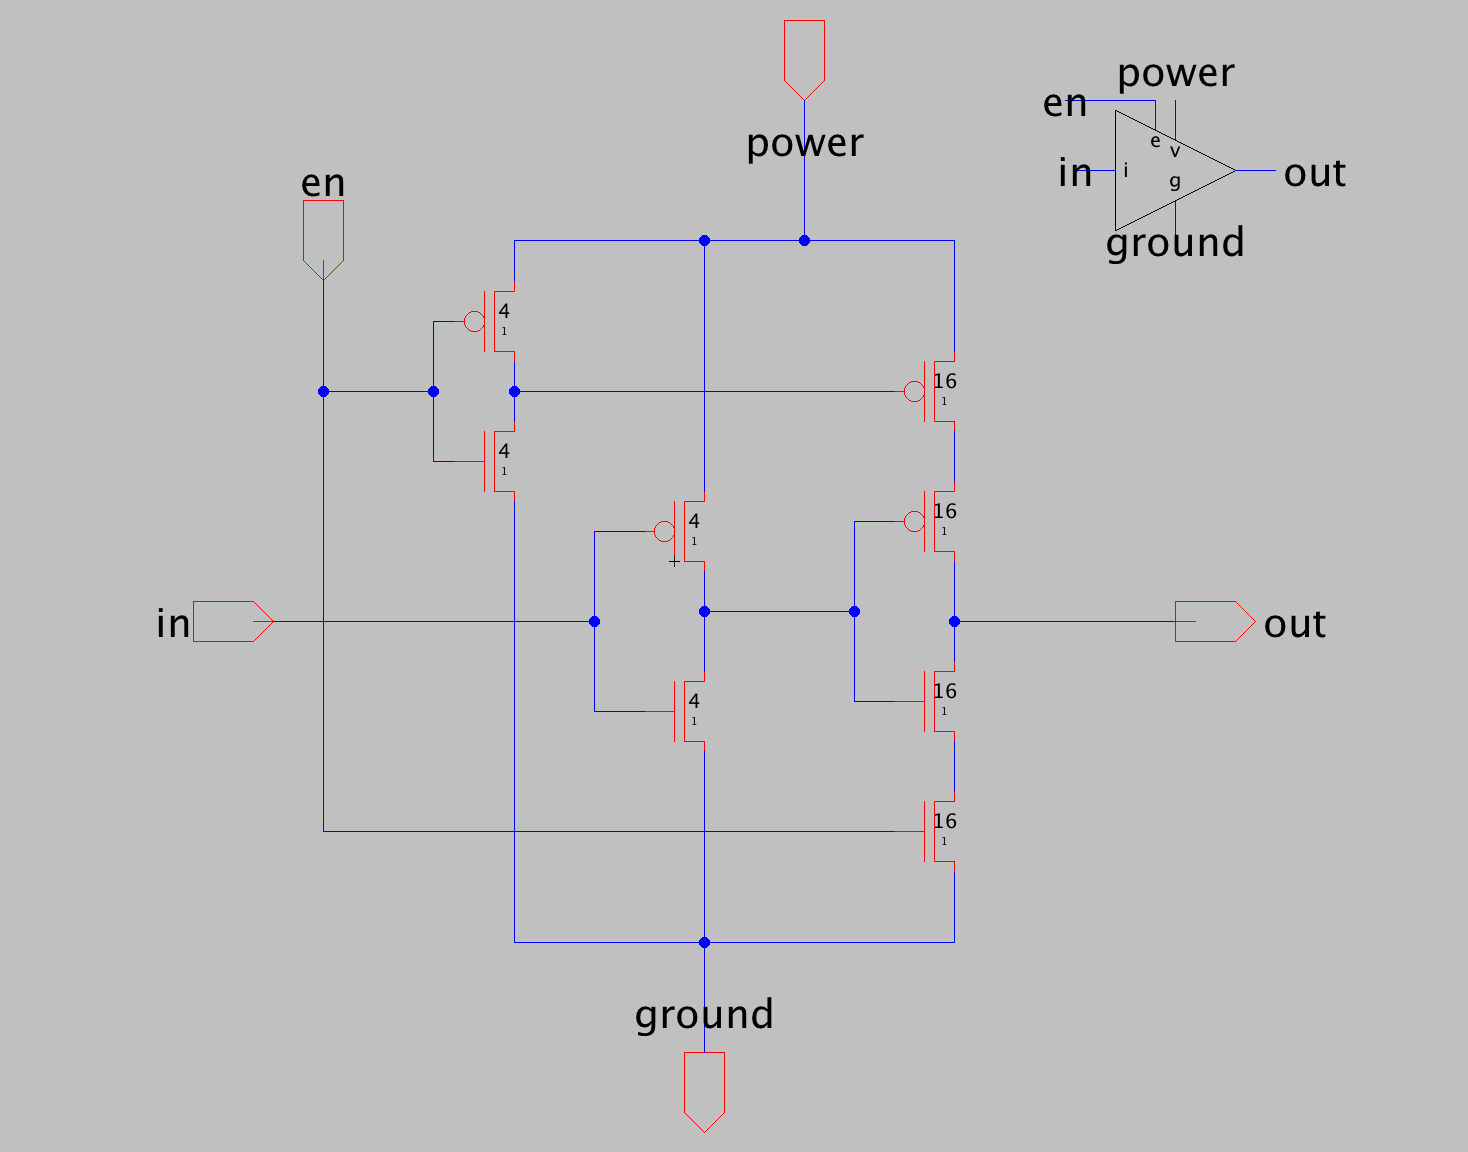
\includegraphics[scale=0.15]{tristate}
	\caption{Tri-State Buffer}
	\label{fig:tristate}
\end{figure}

\begin{figure}[H]
	\centering
	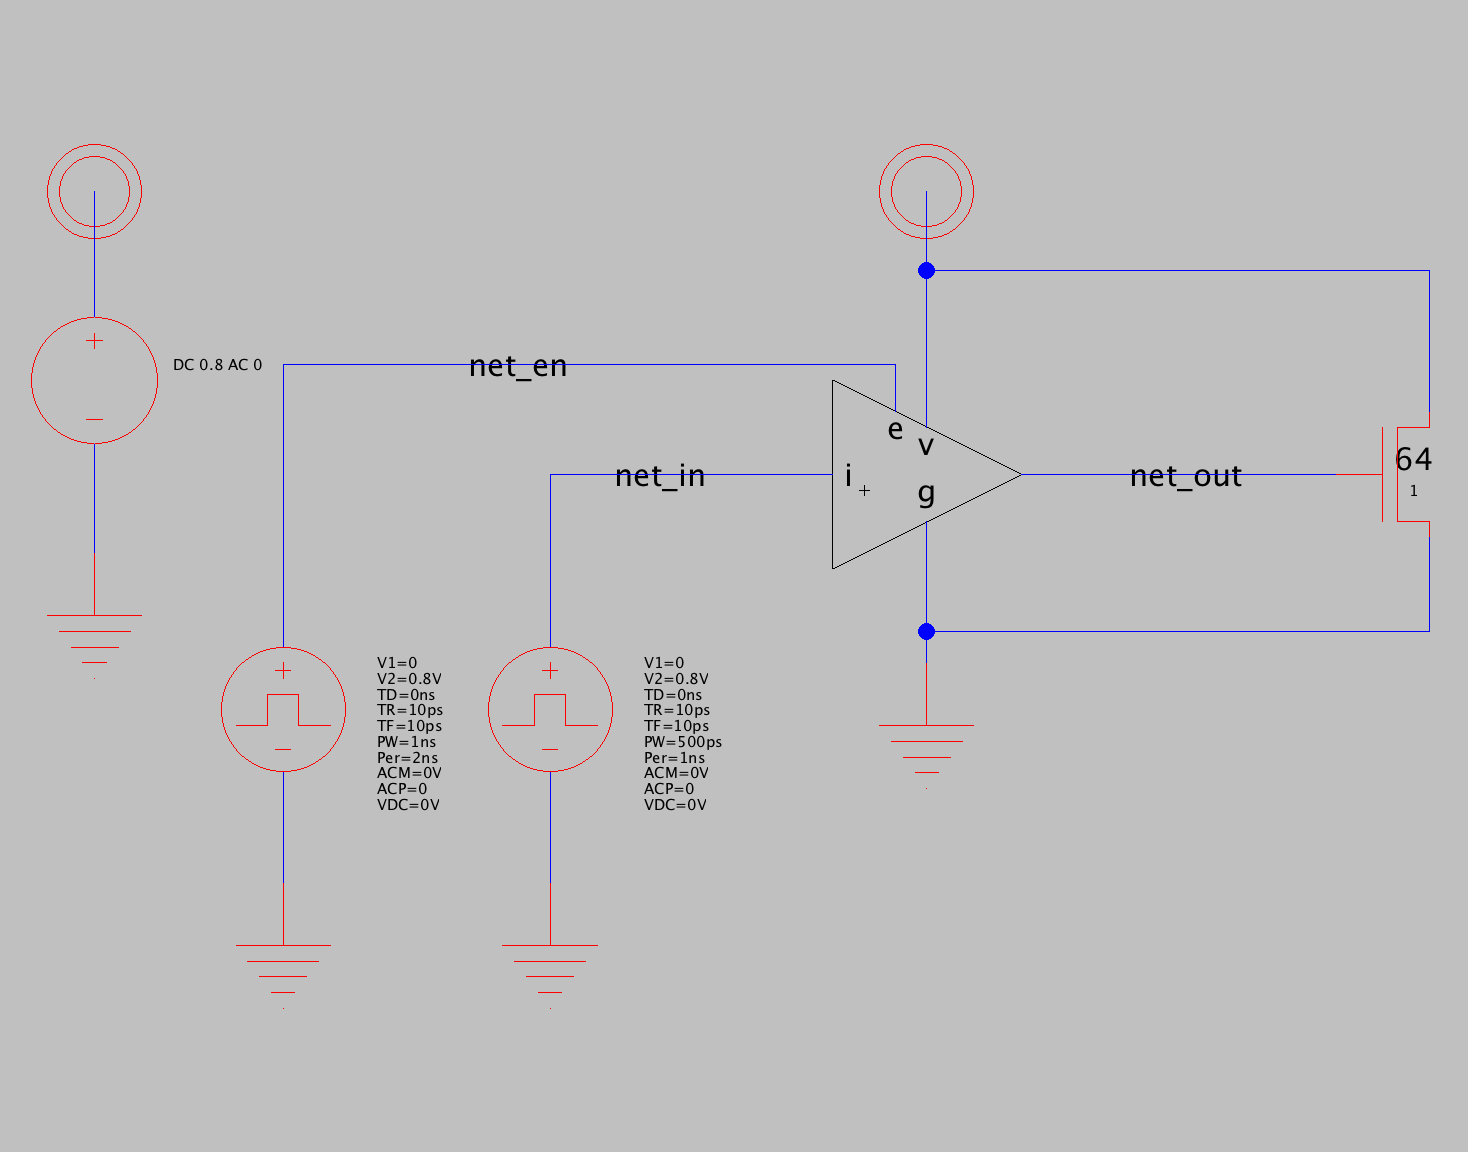
\includegraphics[scale=0.15]{triBufTest}
	\caption{Tri-State Buffer Test Bench}
	\label{fig:triBufTest}
\end{figure}

Finally, below is the waveform which shows our circuit working properly as it should wherein the output is pushed to the according driving value only when the enable is high.

\begin{figure}[H]
	\centering
	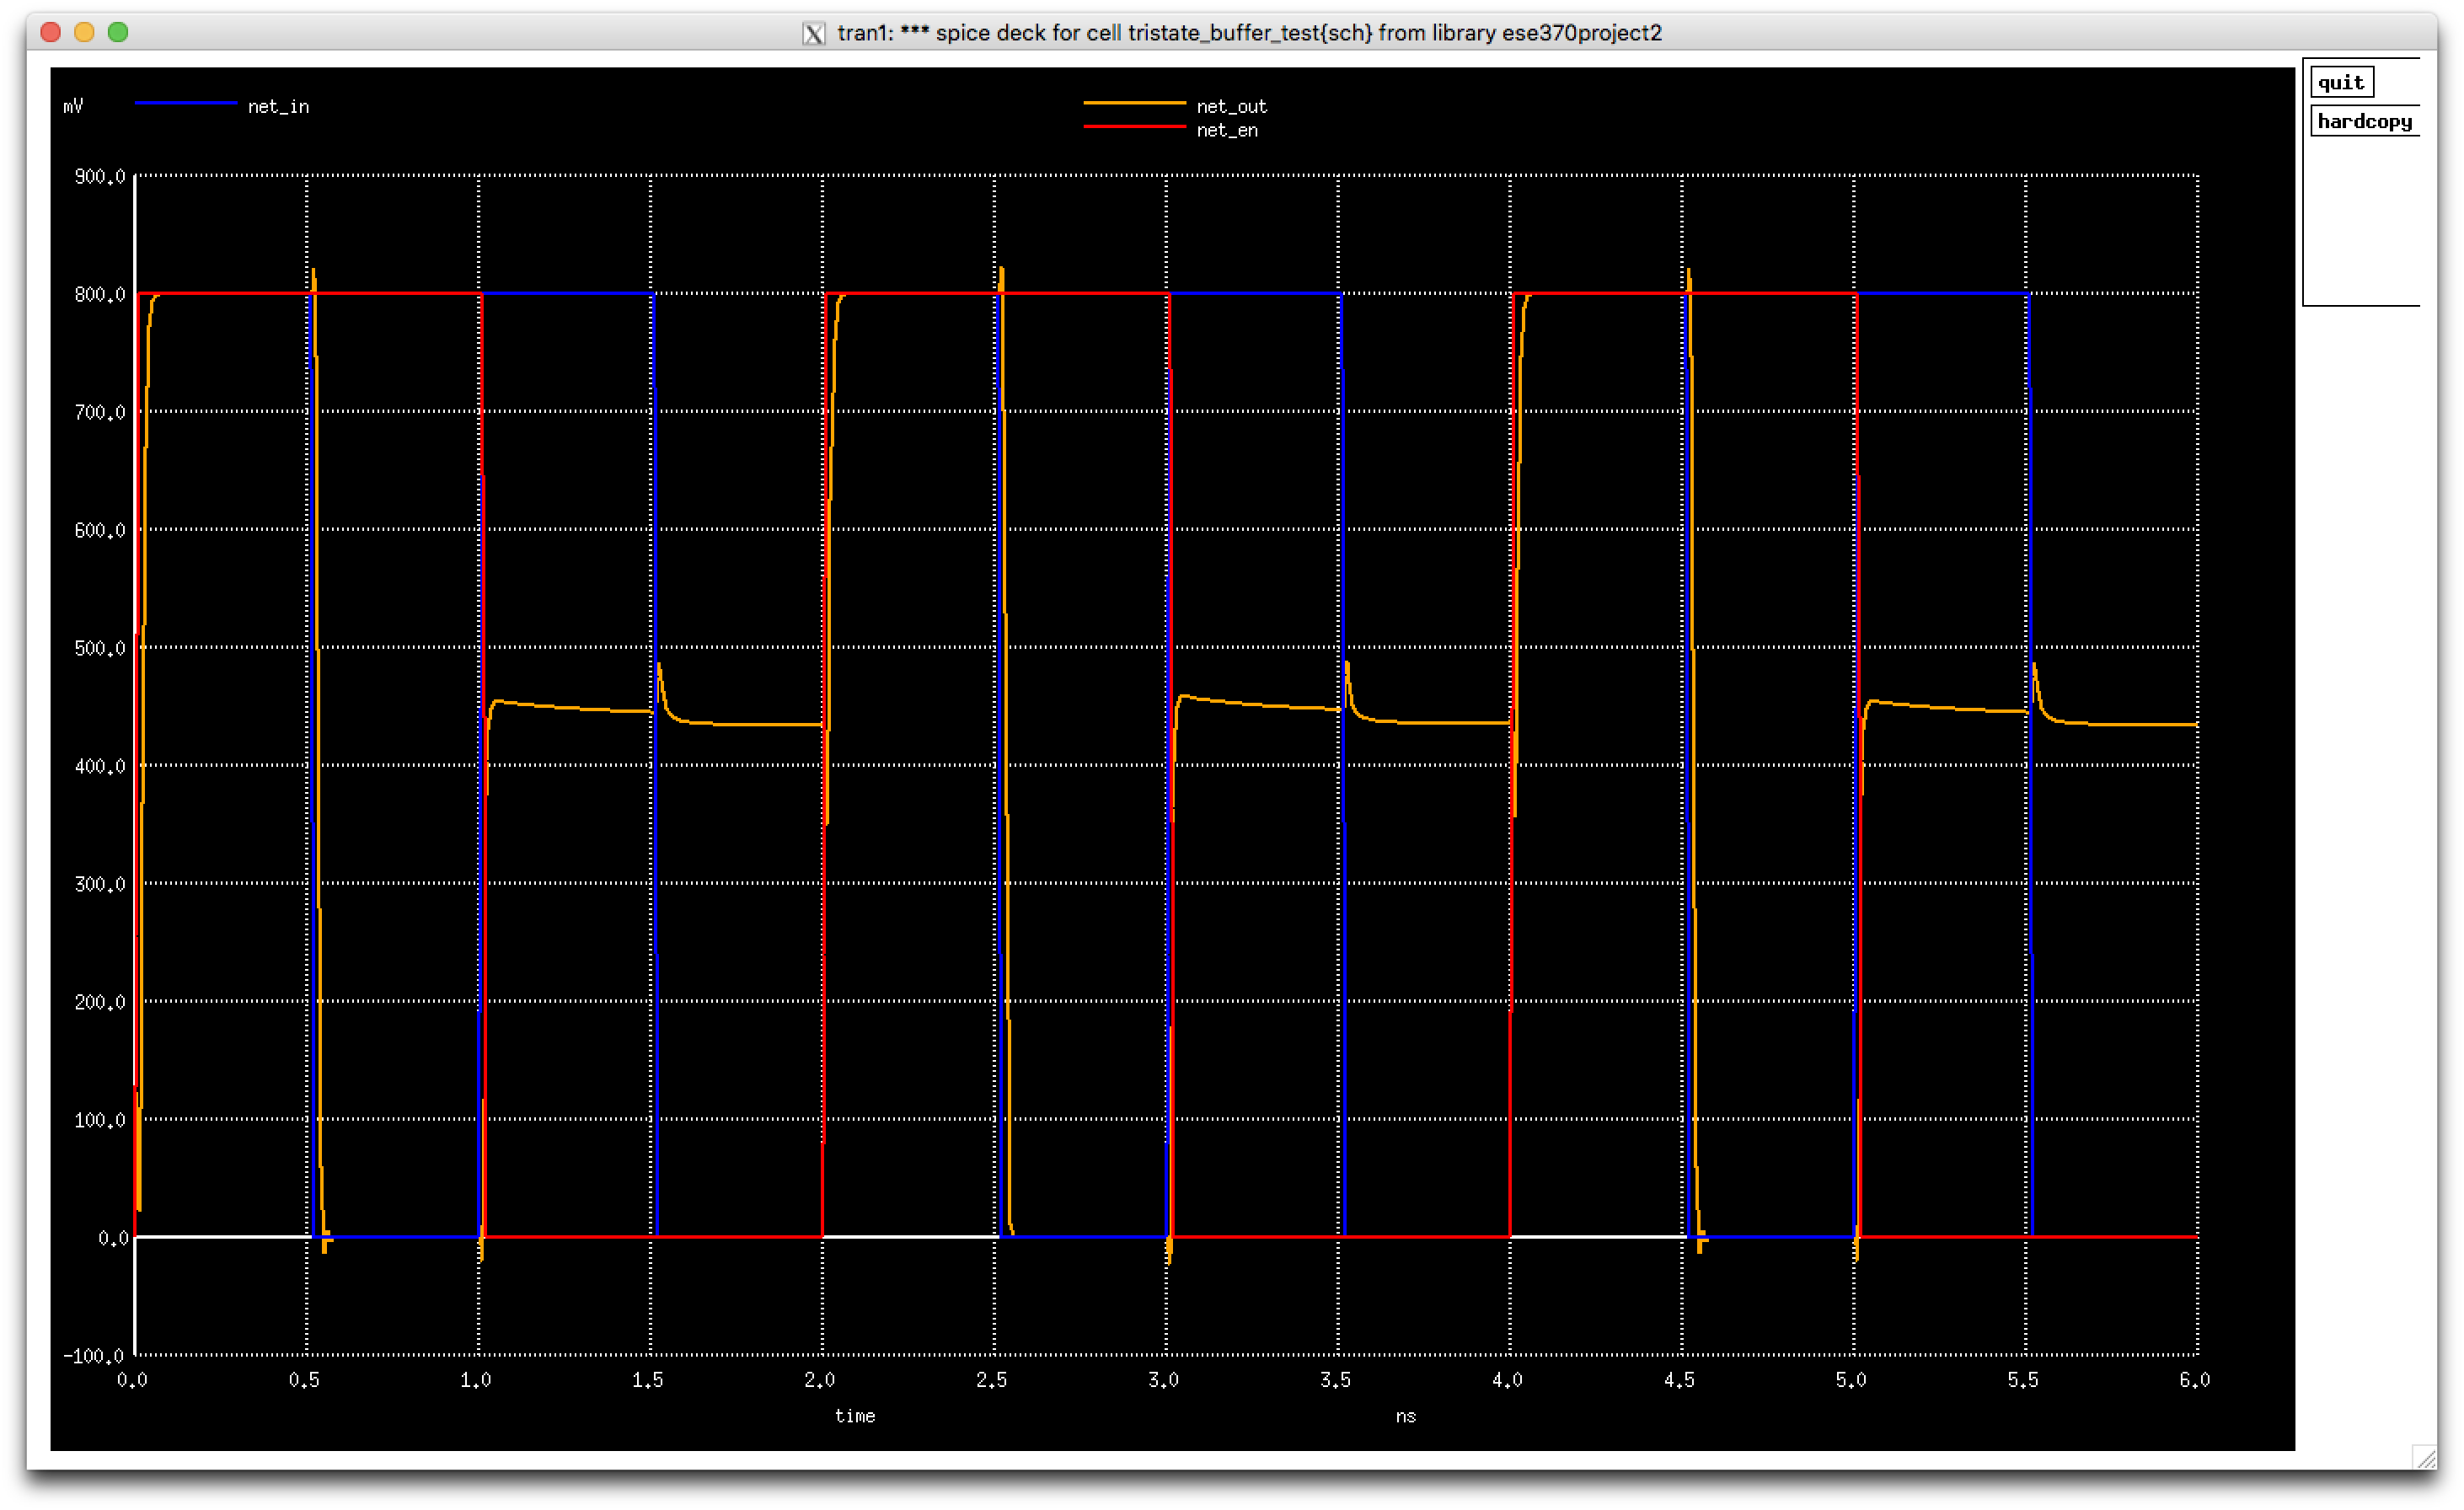
\includegraphics[scale=0.15]{triBufWave}
	\caption{Tri-State Buffer Test Bench Waveform}
	\label{fig:triBufWave}
\end{figure}

\subsubsection{Complete Bit Line}
First, we created an entire bitline to test, but after realizing that we only needed to read from and write to a single memory cell to test the entire bitline, we decided to re-size a transistor to mimick the load of the rest of the memory cells. The schematics are shown below: 
\begin{figure}[H]
	\centering
	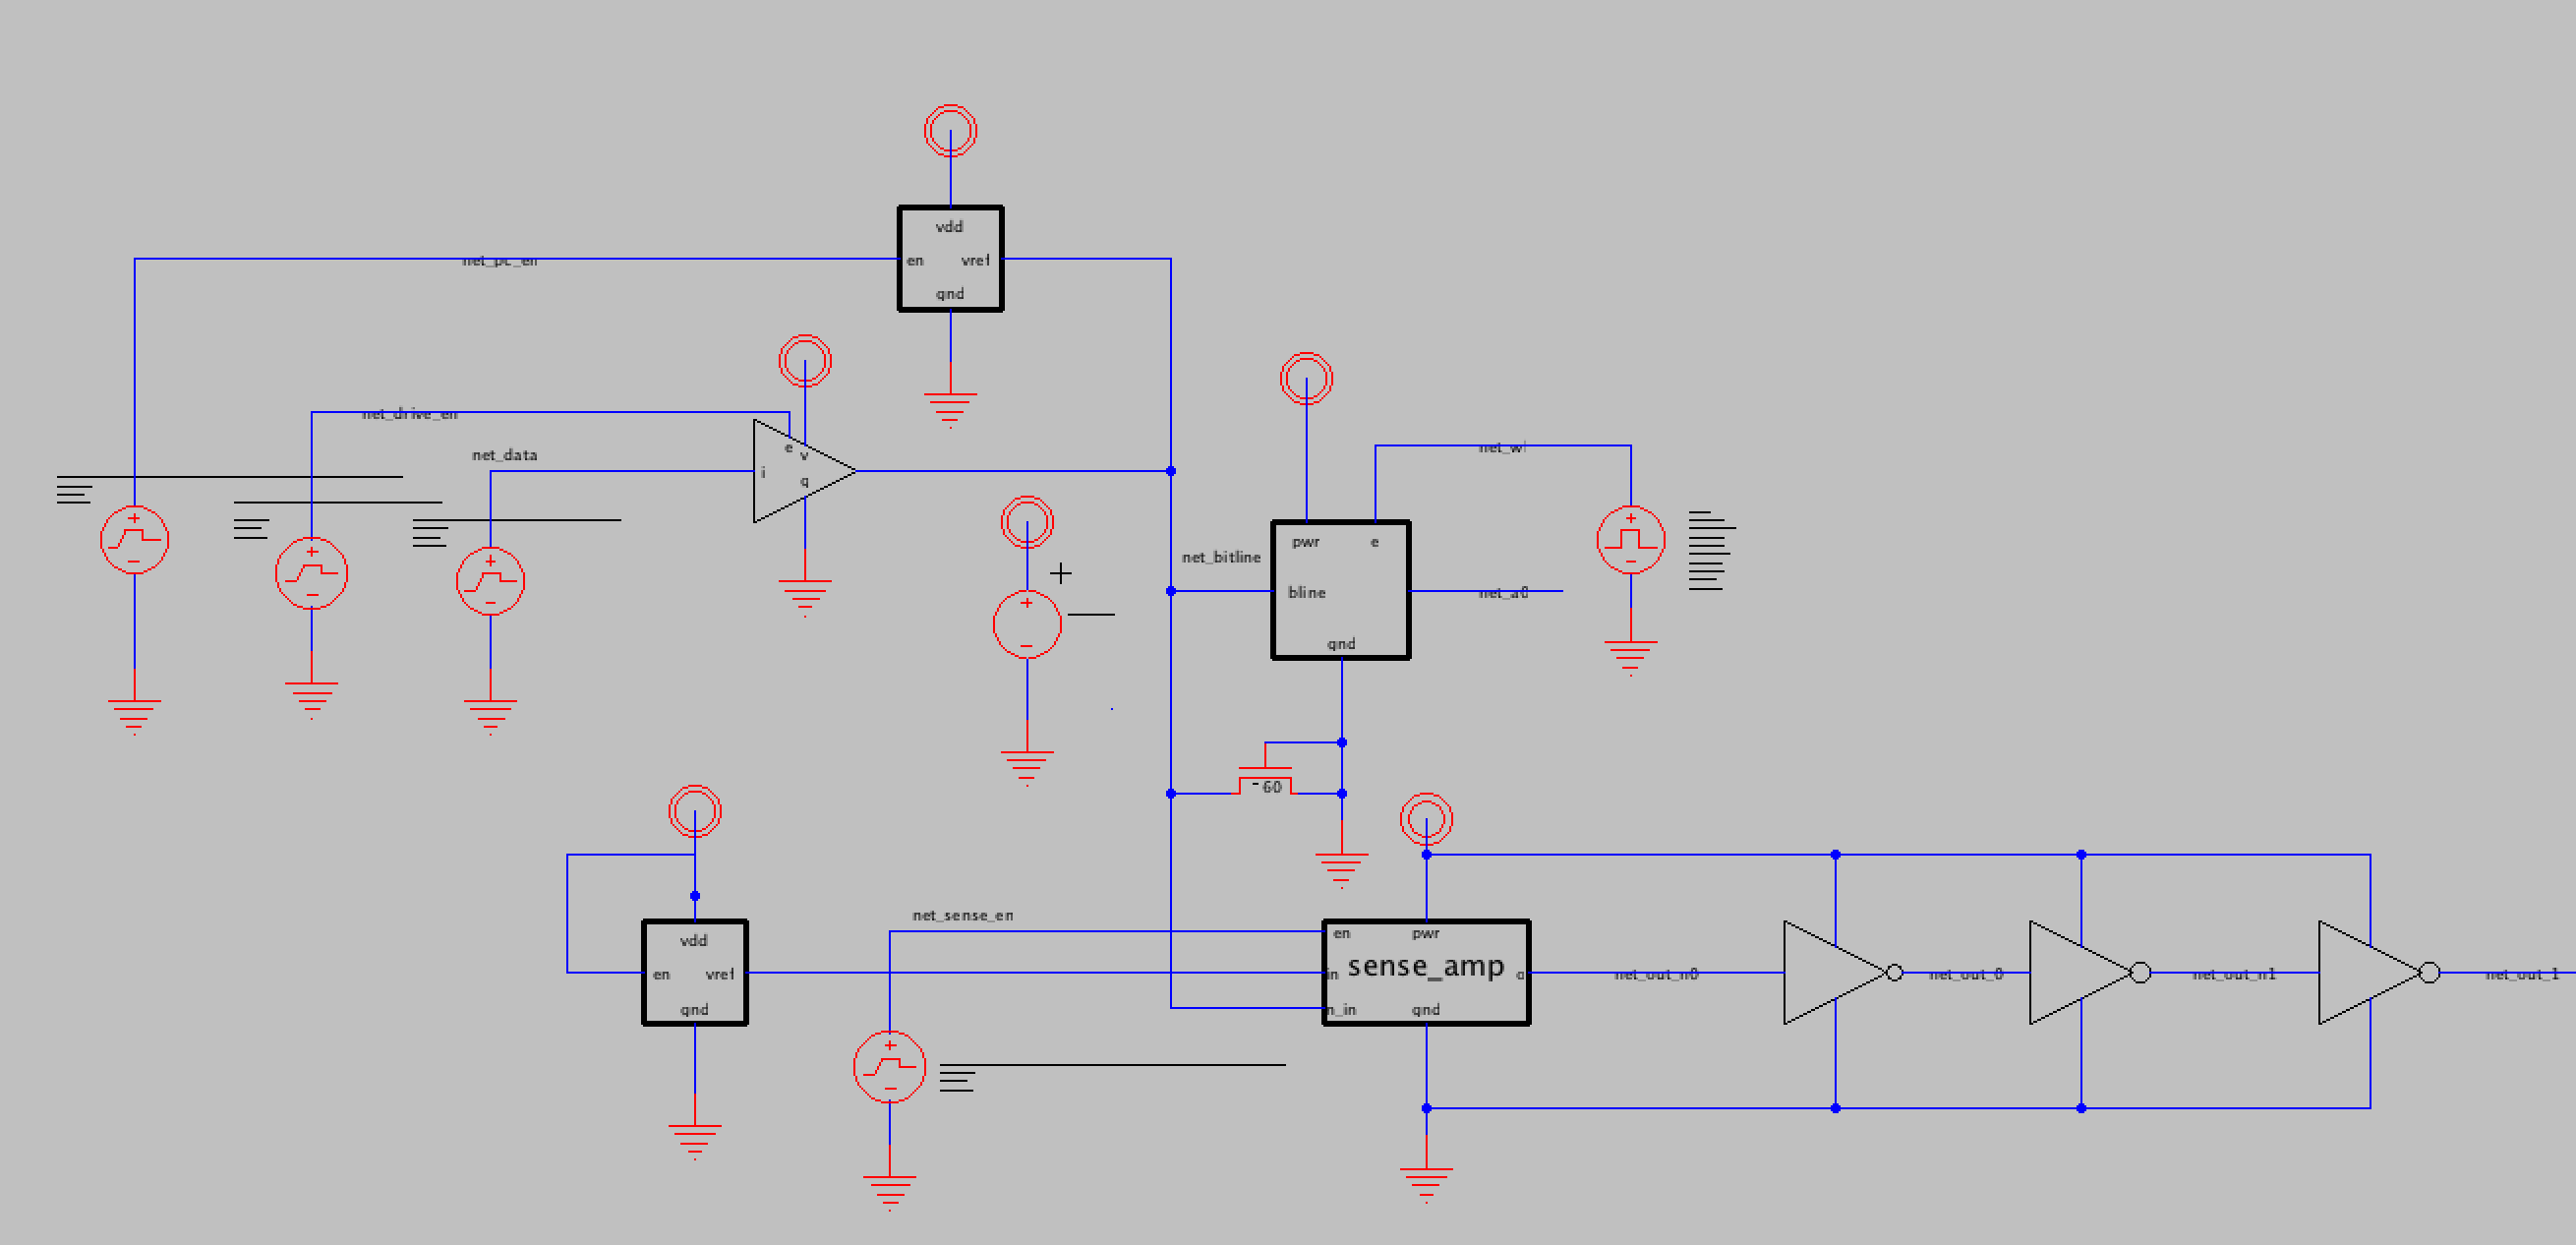
\includegraphics[scale=0.25]{exampleBitlineFull}
	\caption{Full Schematic}
	\label{fig:bitlineFull}
\end{figure}

\begin{figure}[H]
	\centering
	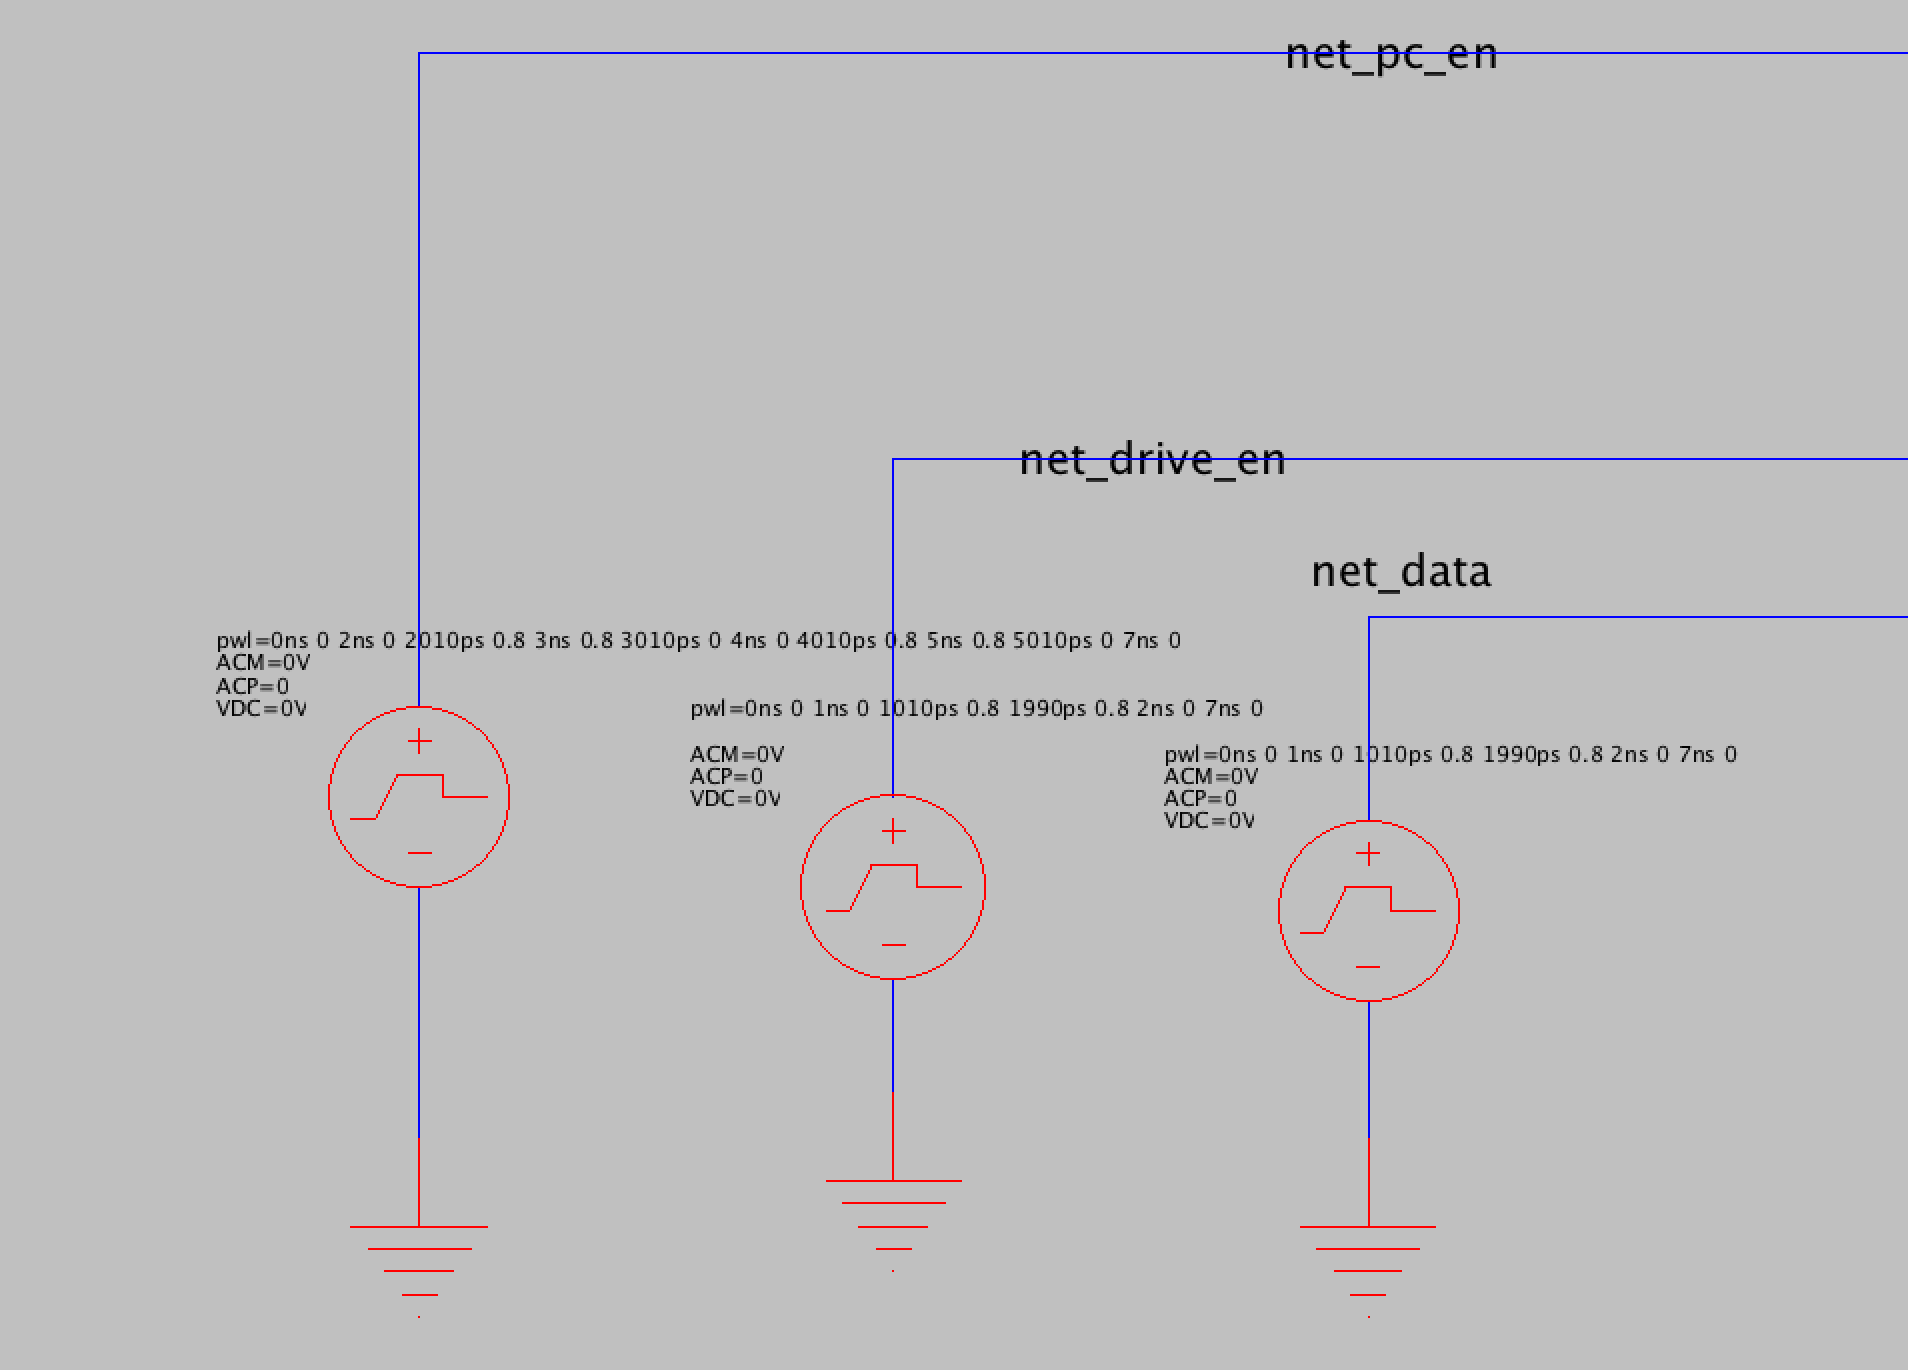
\includegraphics[scale=0.35]{exampleBitlineInputs}
	\caption{Inputs to Pre-Charge and Tri-State Buffer}
	\label{fig:bitlineInputs}
\end{figure}

\begin{figure}[H]
	\centering
	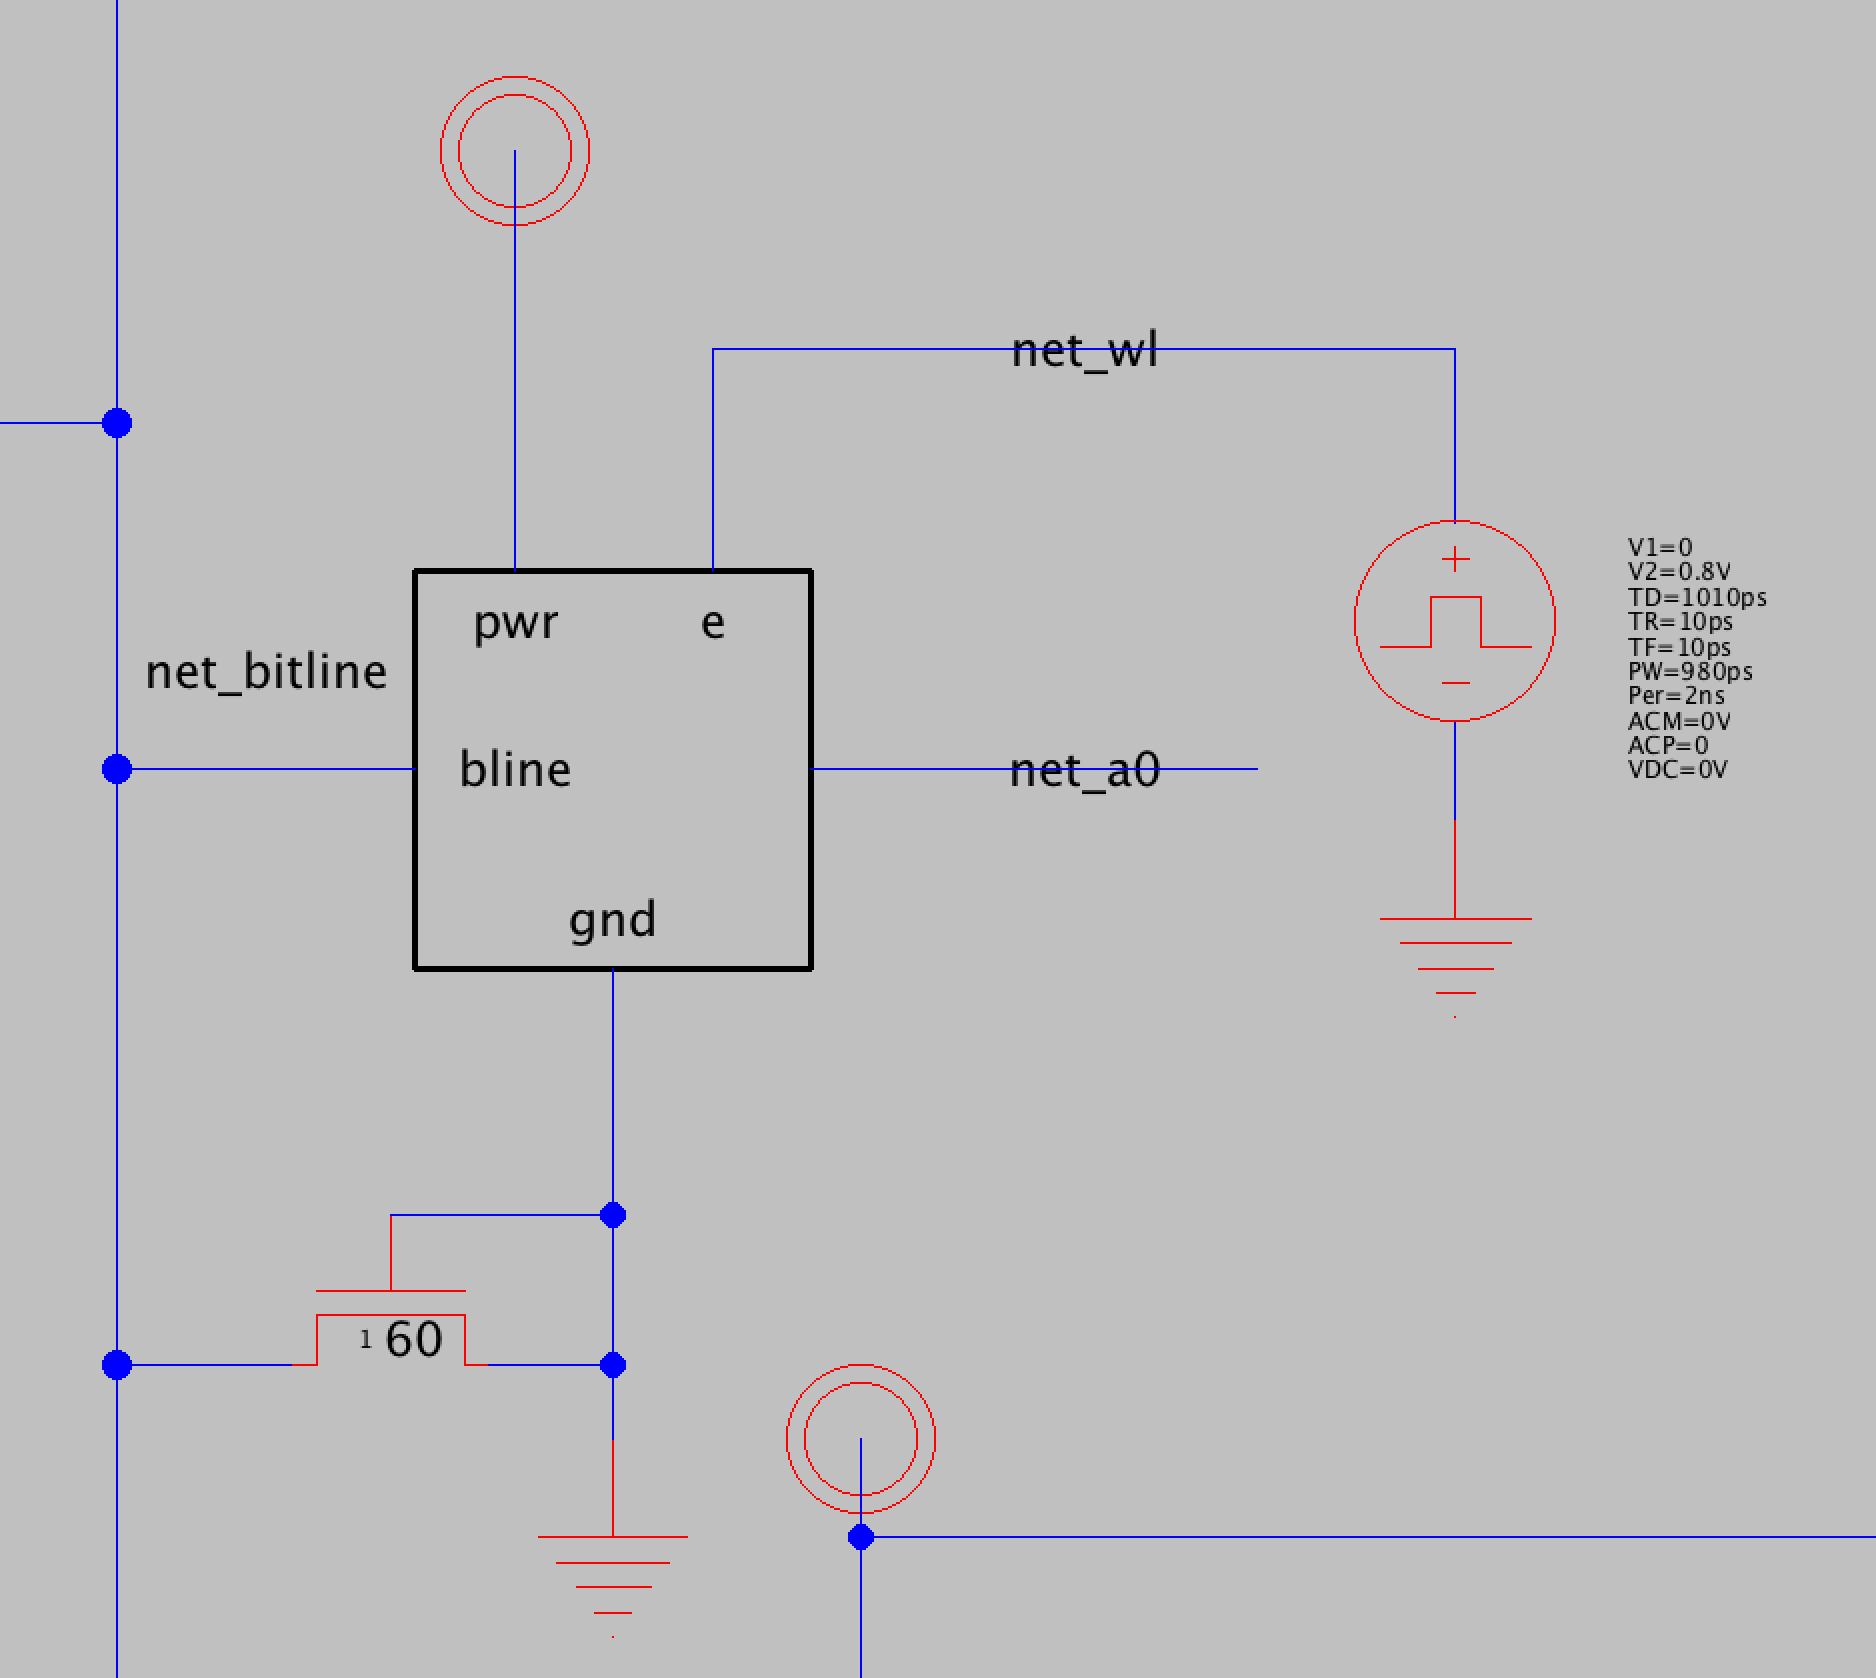
\includegraphics[scale=0.3]{exampleBitlineMemoryCell}
	\caption{Memory Cell and Sized Load Transistor}
	\label{fig:bitlineMemCell}
\end{figure}

\begin{figure}[H]
	\centering
	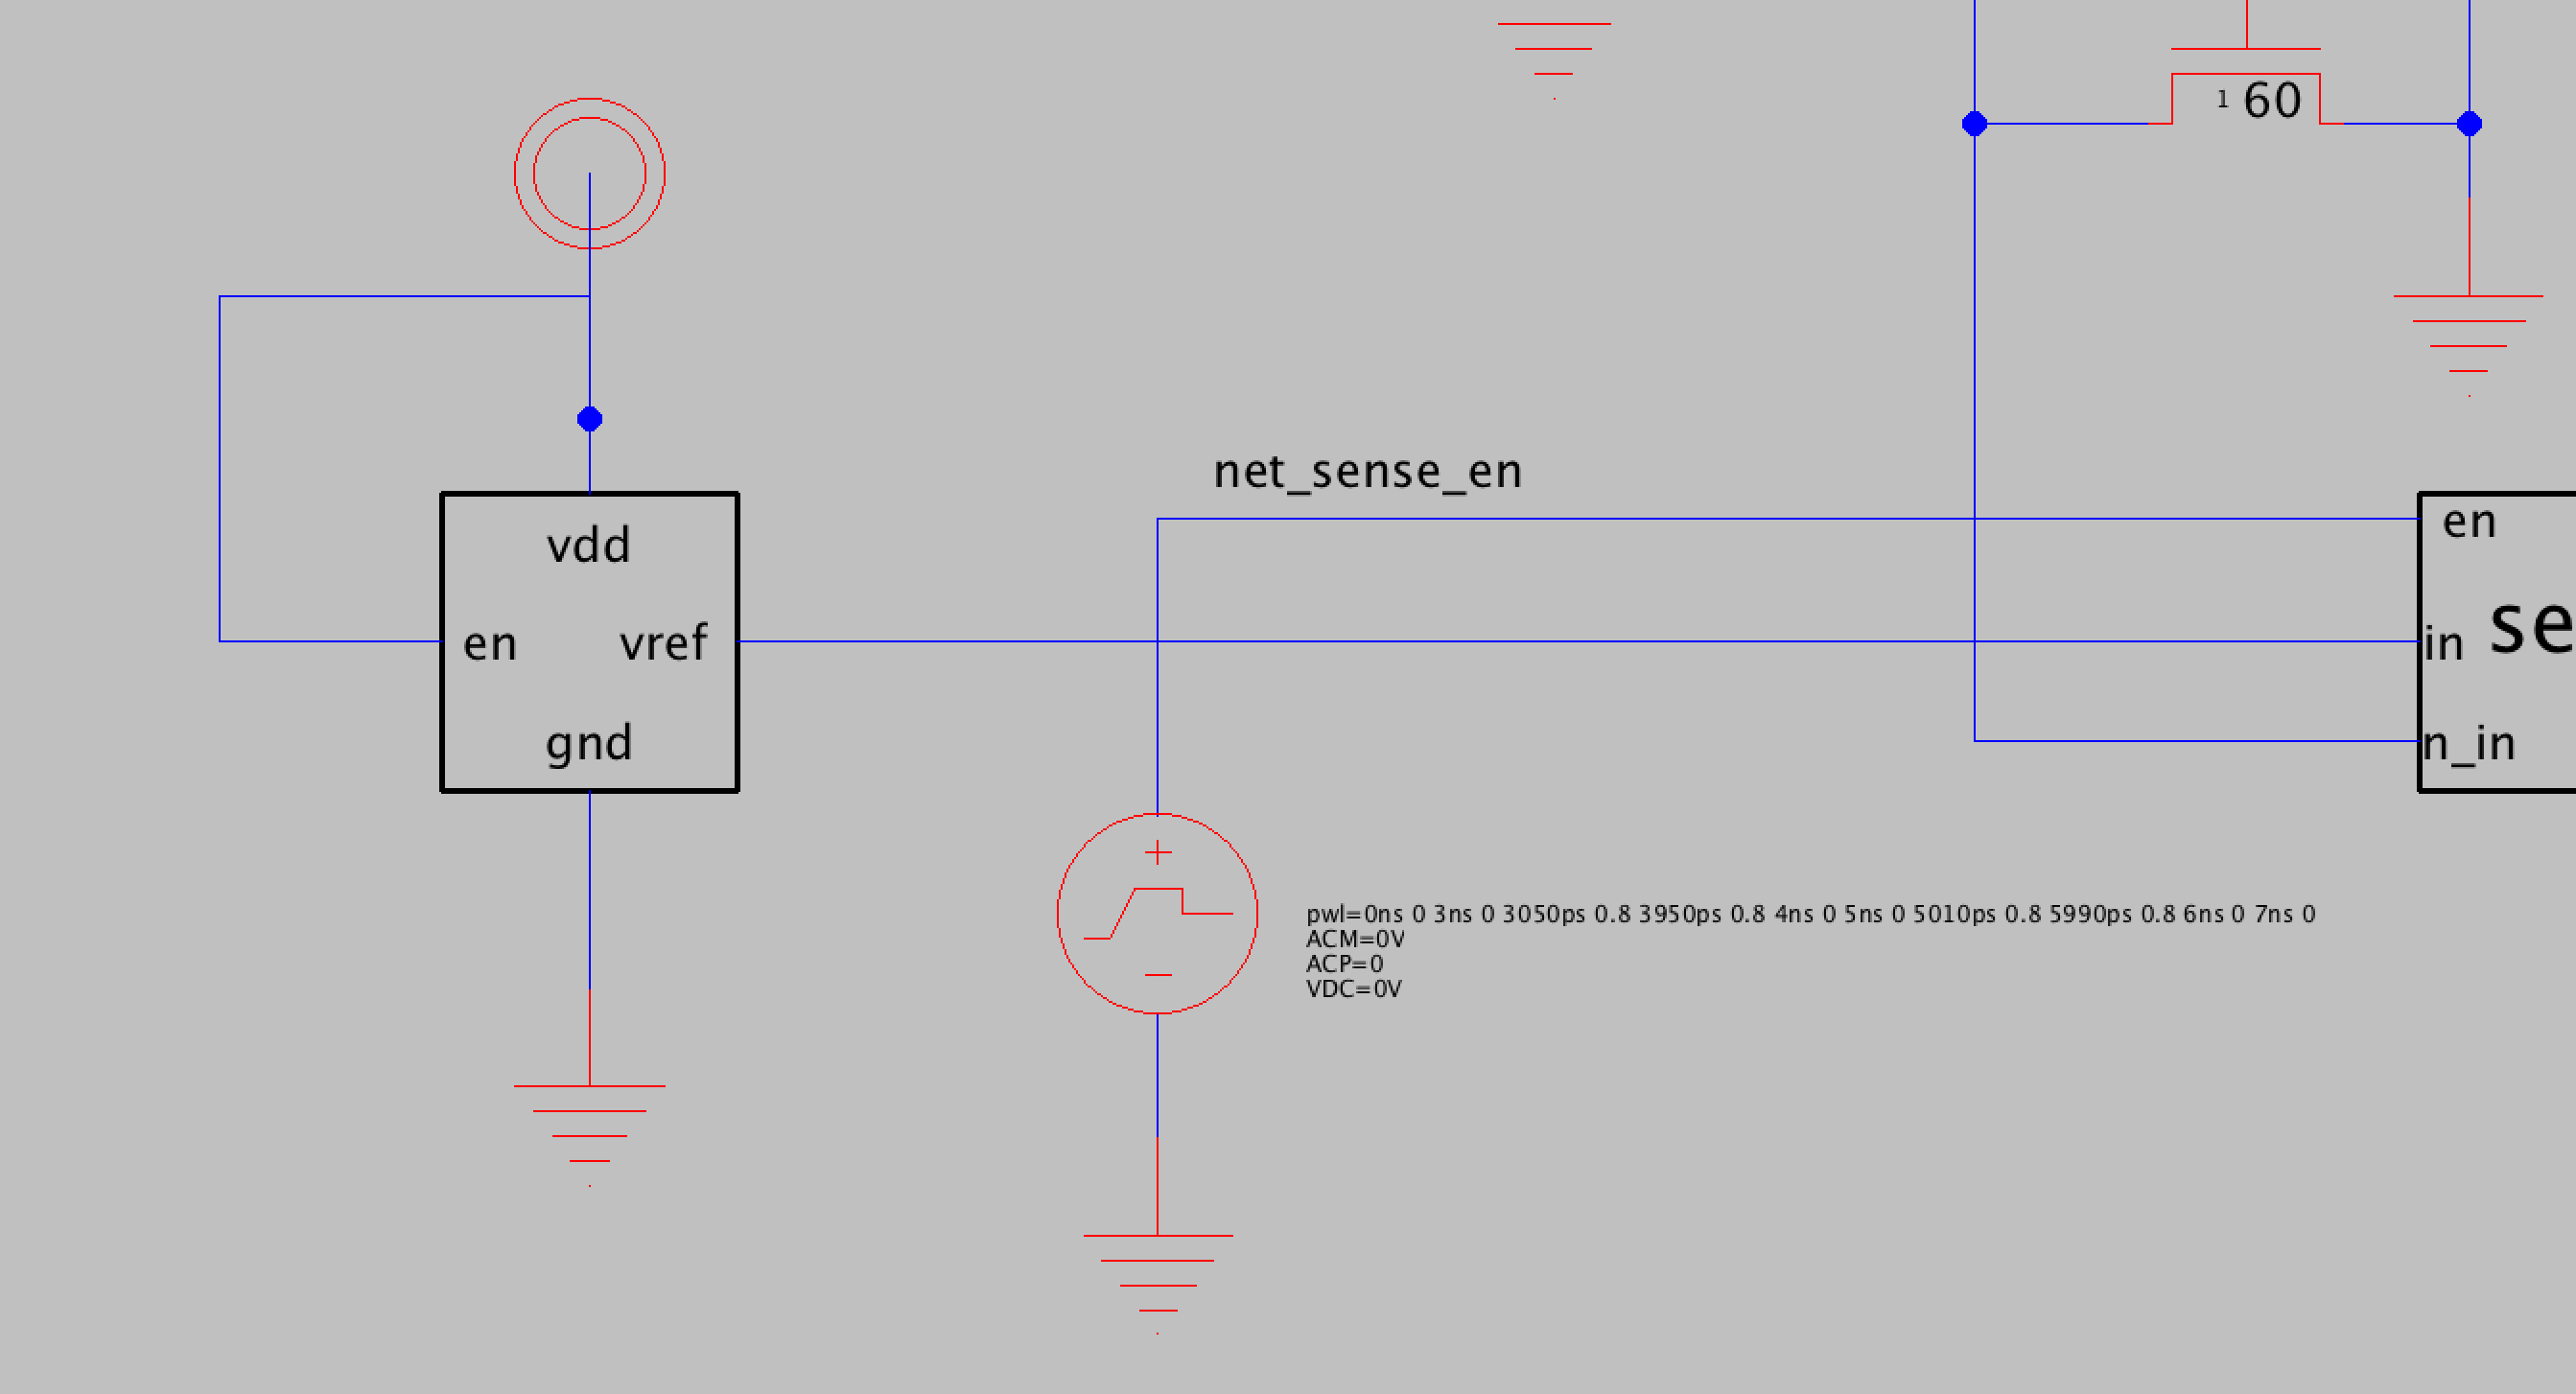
\includegraphics[scale=0.25]{exampleBitlineSenseInputs}
	\caption{Differential Sense Amplifier Inputs}
	\label{fig:bitlineSenseInputs}
\end{figure}

\begin{figure}[H]
	\centering
	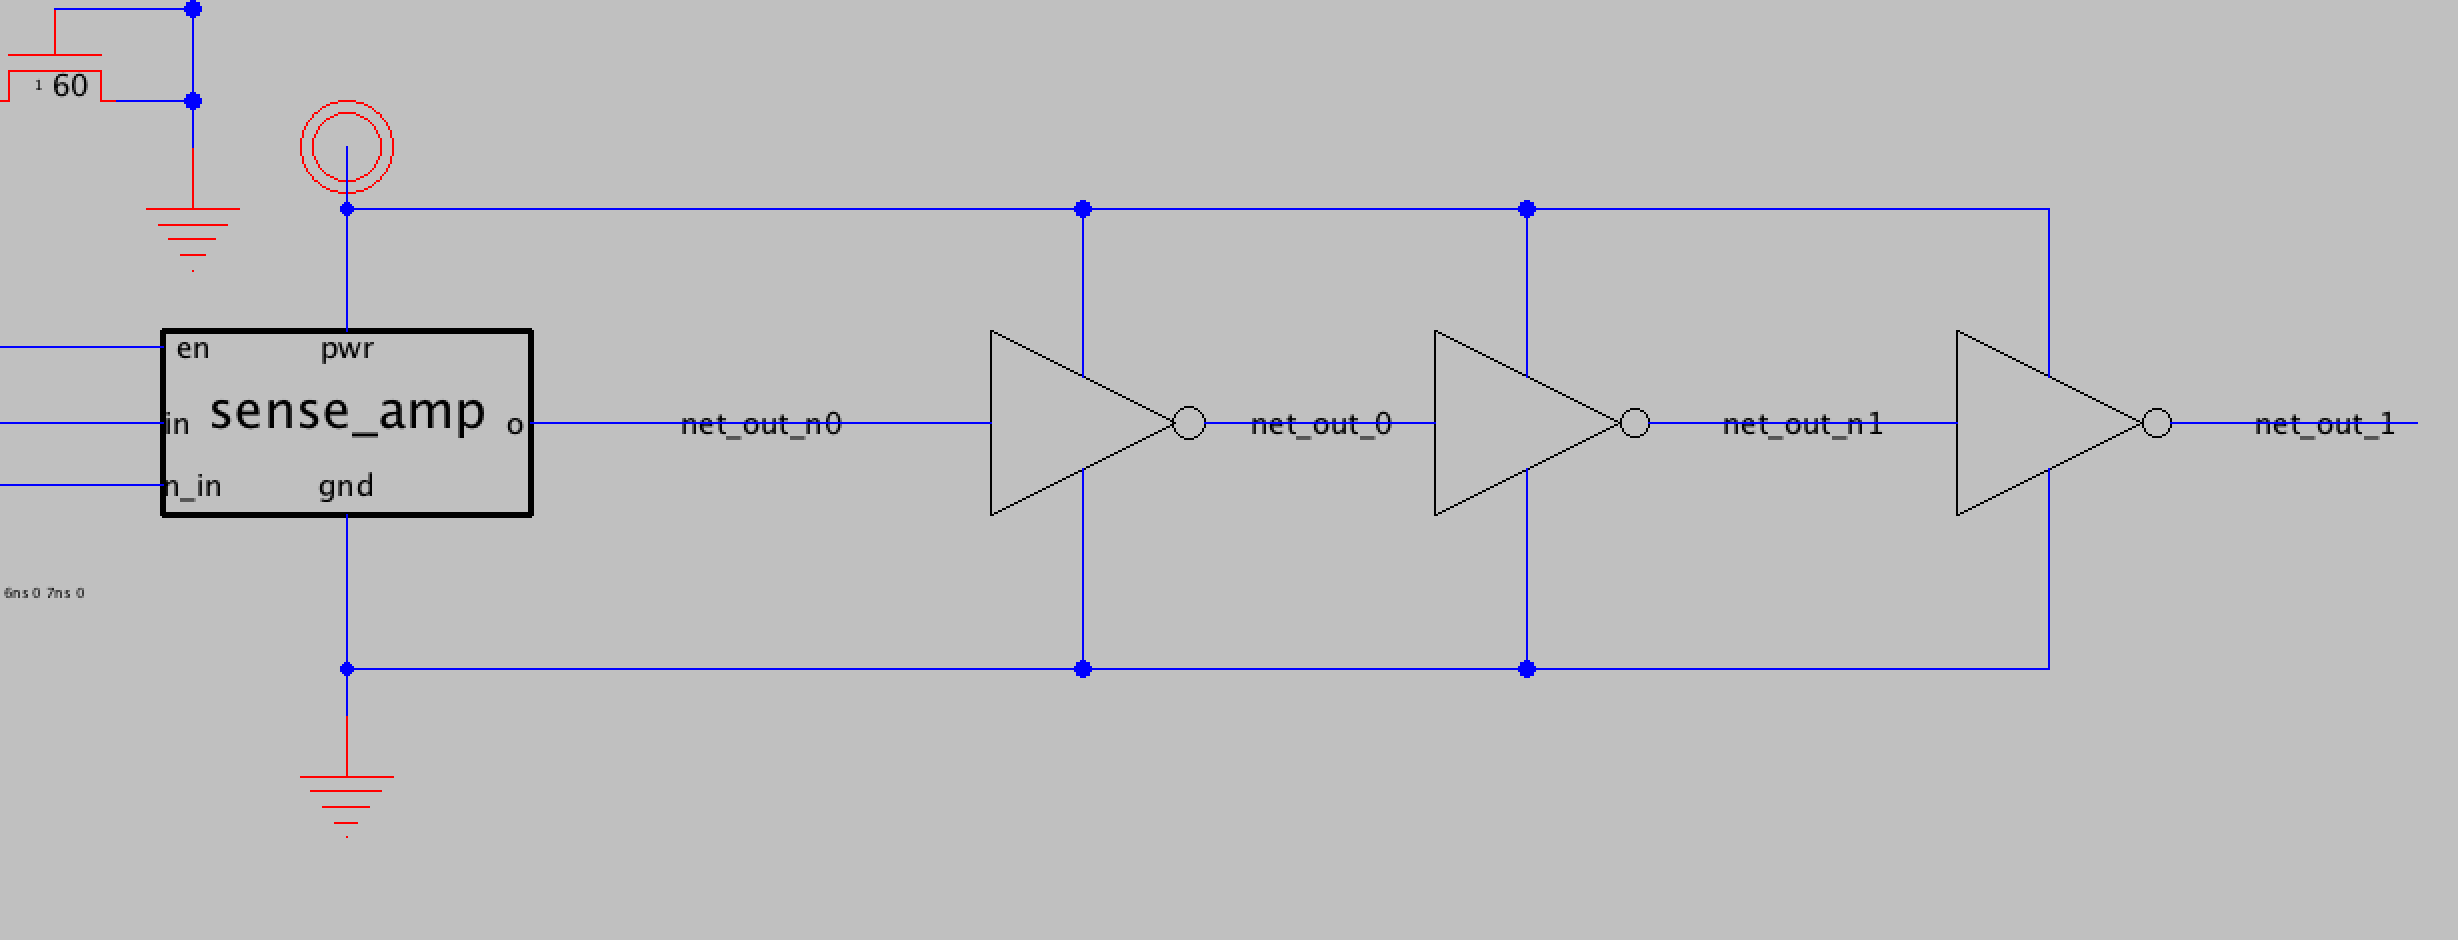
\includegraphics[scale=0.3]{exampleBitlineOutputs}
	\caption{Output Buffers}
	\label{fig:bitlineOutputs}
\end{figure}

\textbf{Correctness}
The goal is to write a 1 to the memory cell and then read the 1 twice. This ensures that the first read is non-destructive. This target waveform is shown below in Figure \ref{fig:bitlineGoalWave}. The output that we received using the schematics above is shown in Figure \ref{fig:bitlineActualWave}.

\begin{figure}[H]
	\centering
	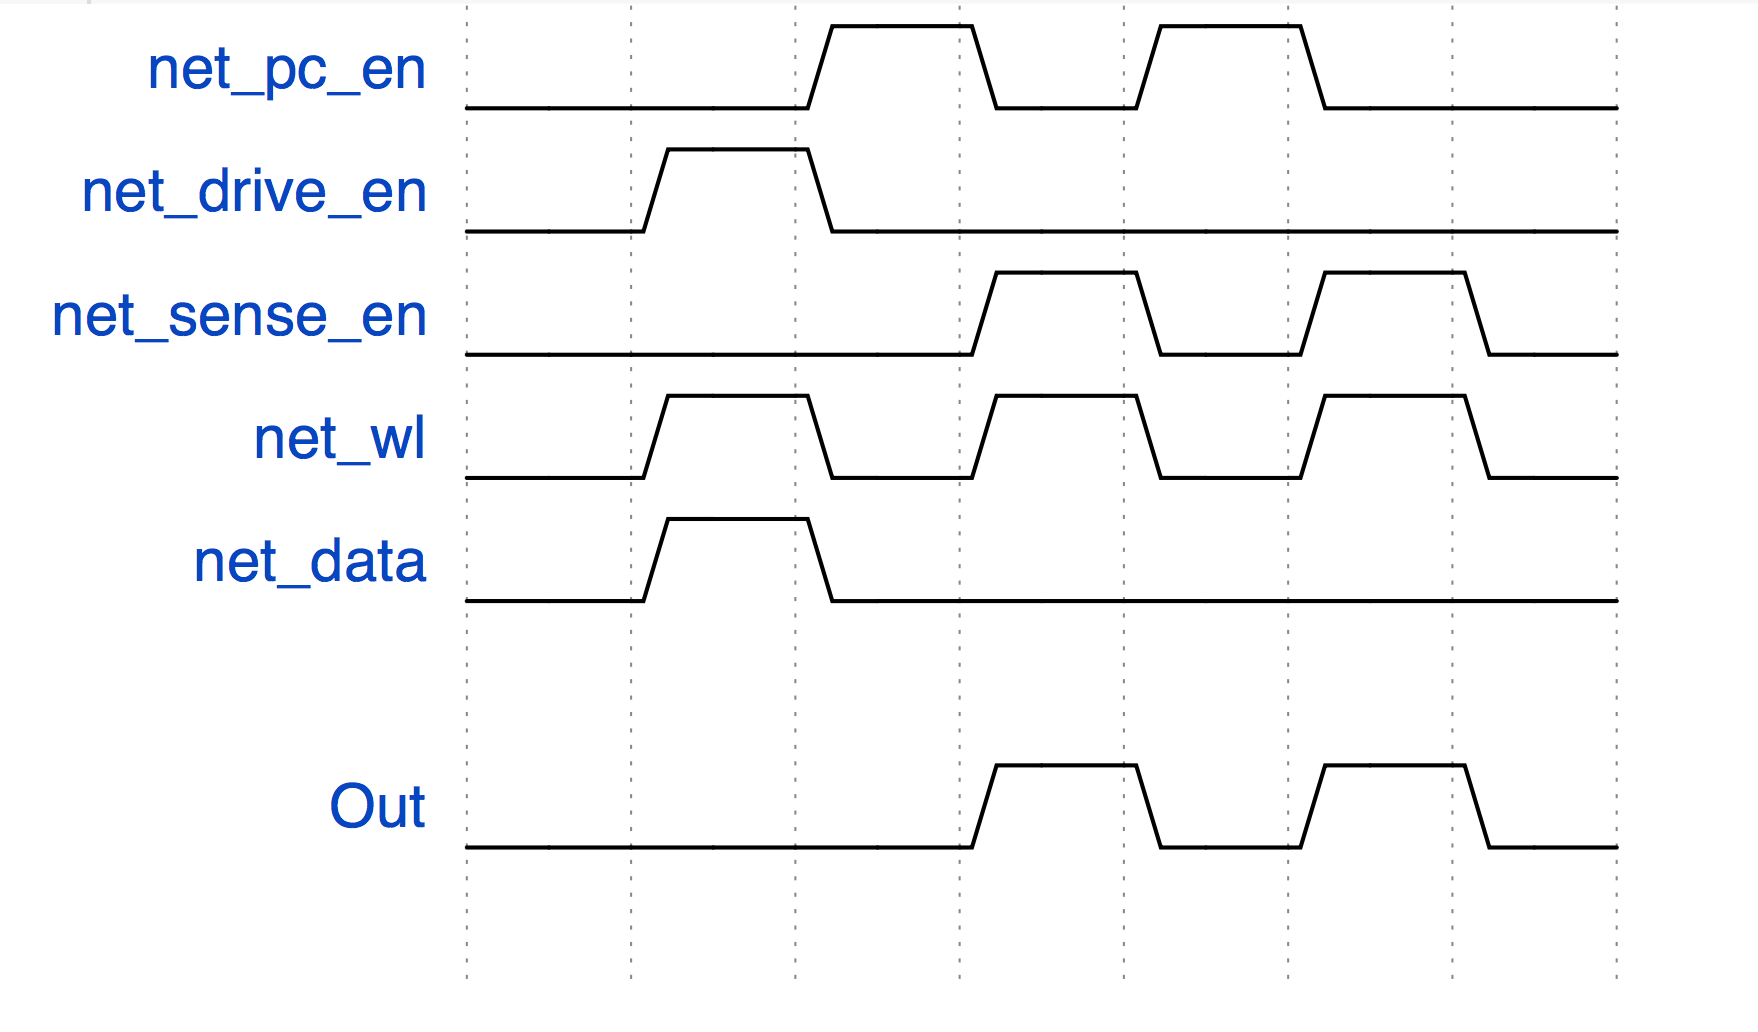
\includegraphics[scale=0.4]{exampleBitlineGoalWaveform}
	\caption{Goal Waveforms for Bitline}
	\label{fig:bitlineGoalWave}
\end{figure}

\begin{figure}[H]
	\centering
	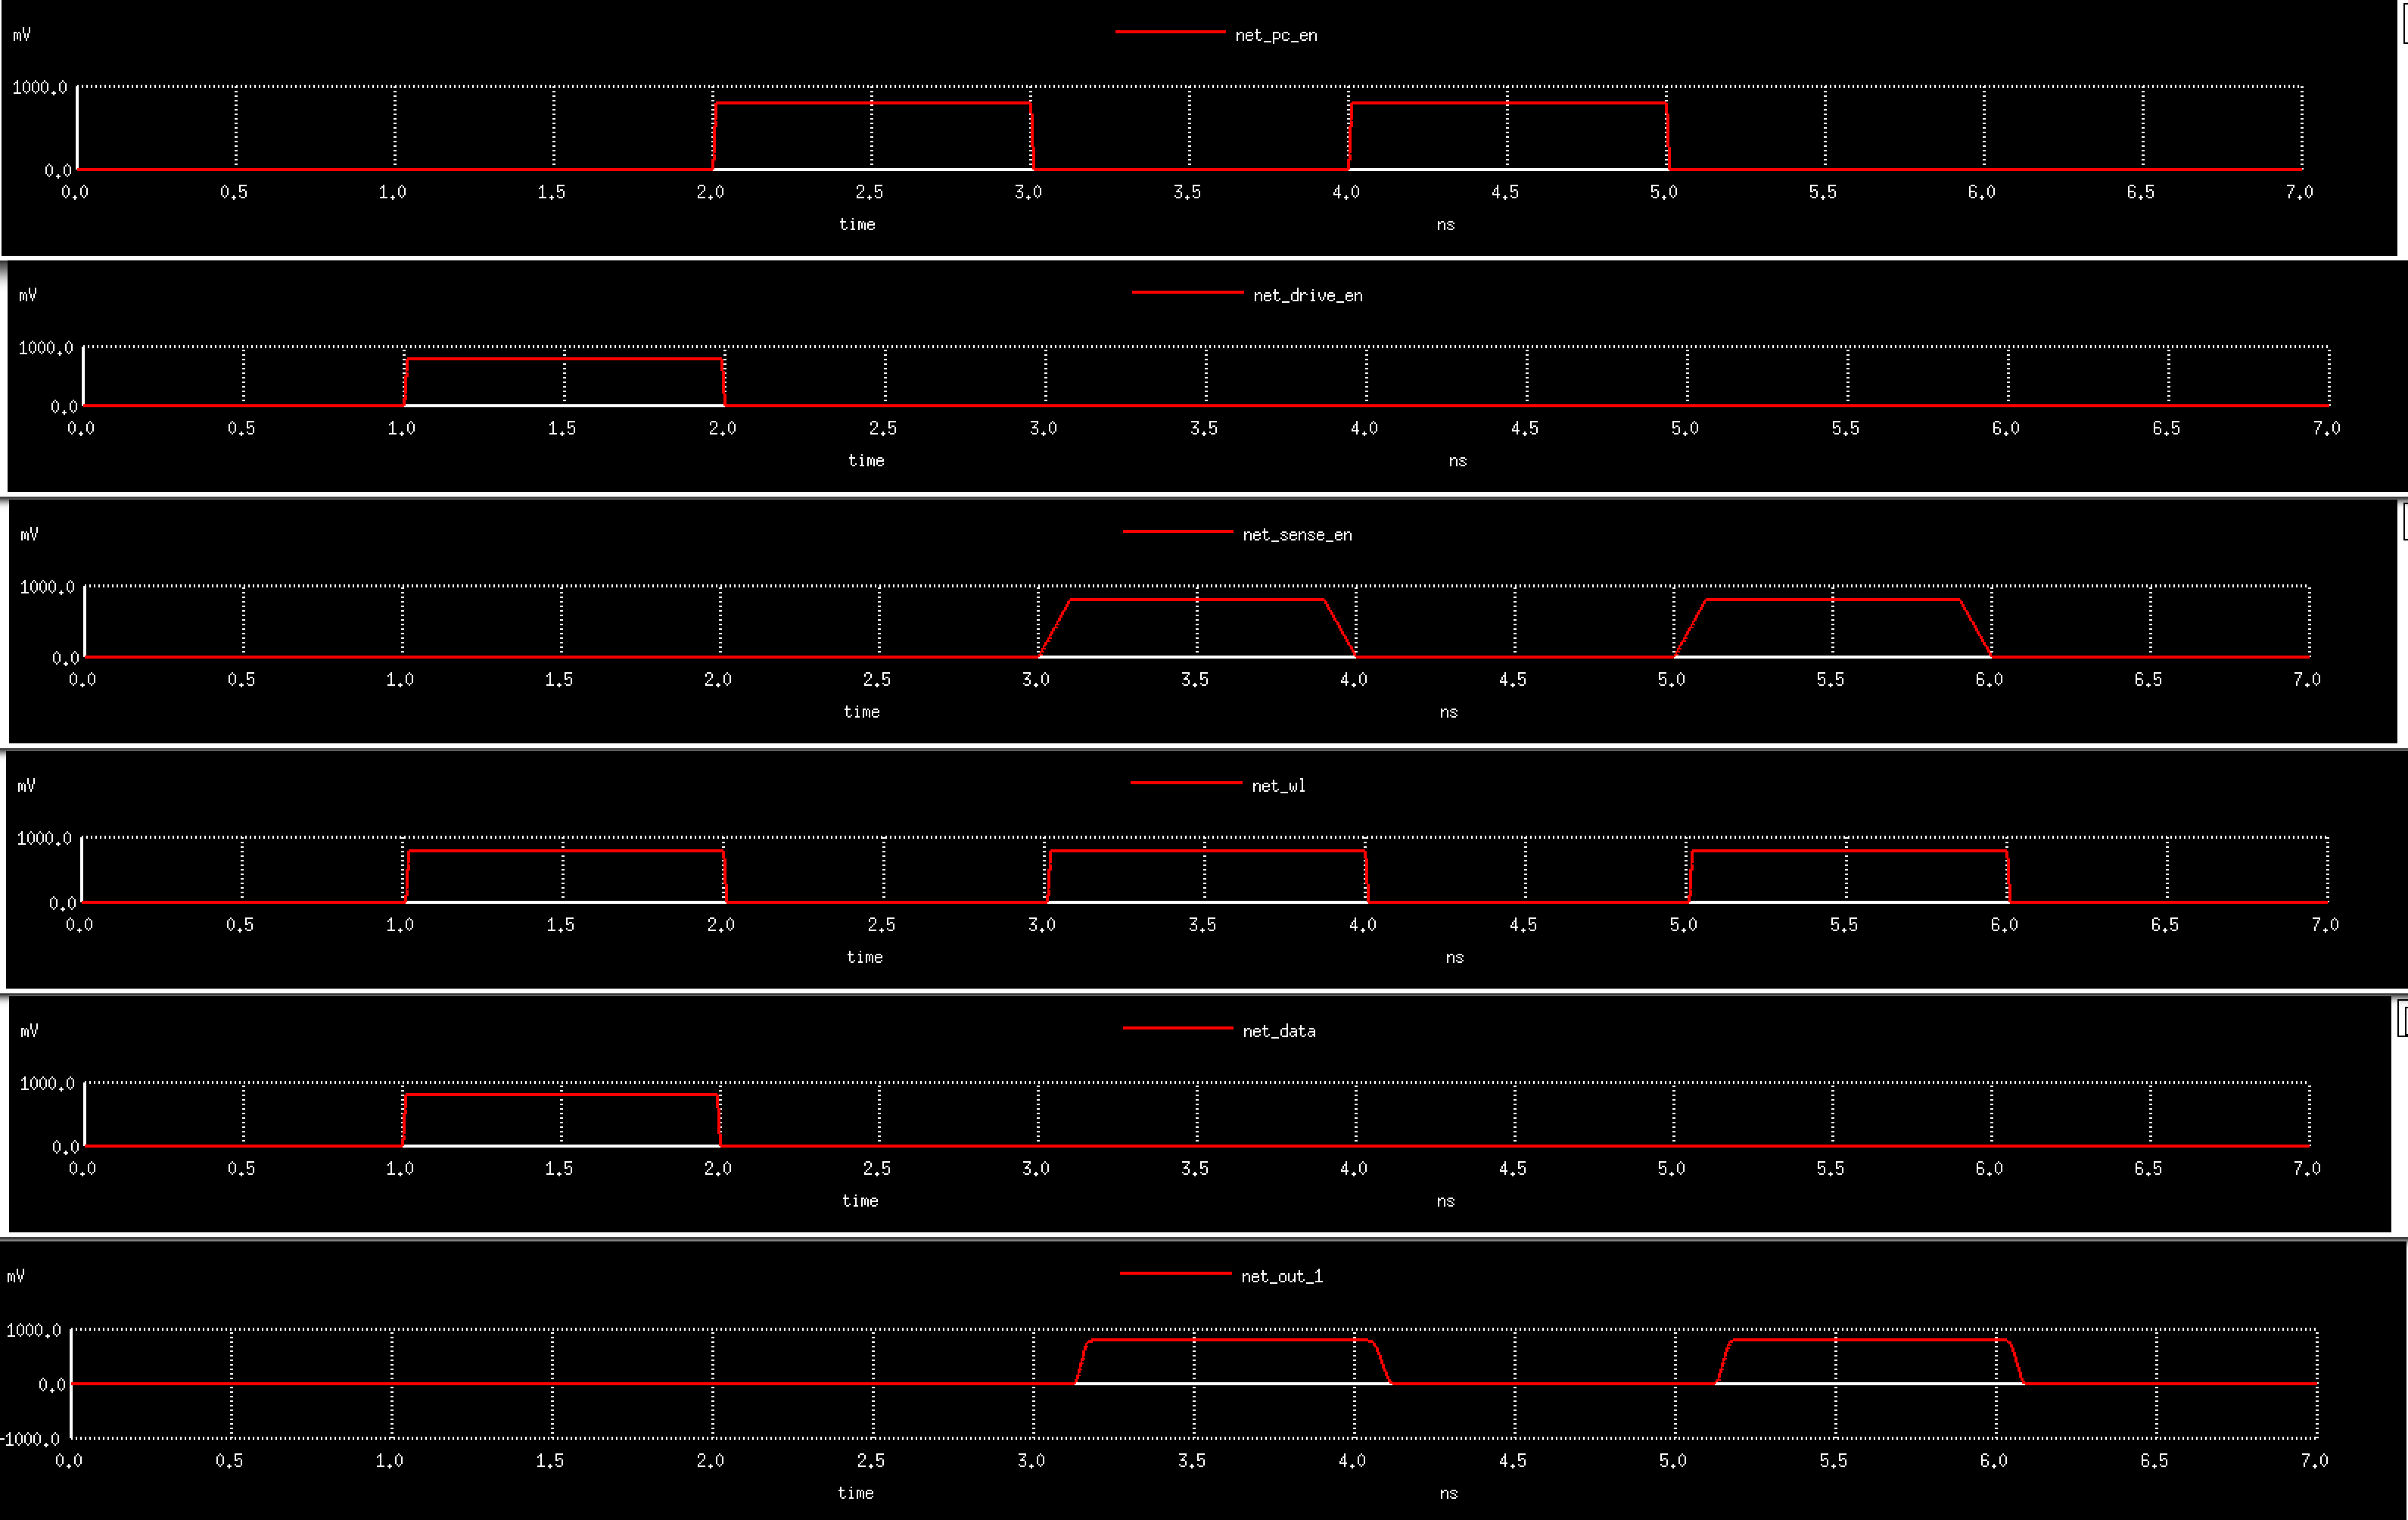
\includegraphics[scale=0.25]{exampleBitlineOutputWaveform}
	\caption{Bitline Output Waveforms}
	\label{fig:bitlineActualWave}
\end{figure}

After validating correctness, we compiled the entire memory cell in the zoomed out schematic of Figure \ref{fig:bitlineLongSchematic1}. This is made of purely 16 of the 5T cells in Figure \ref{fig:5TCell}.

\begin{figure}[H]
	\centering
	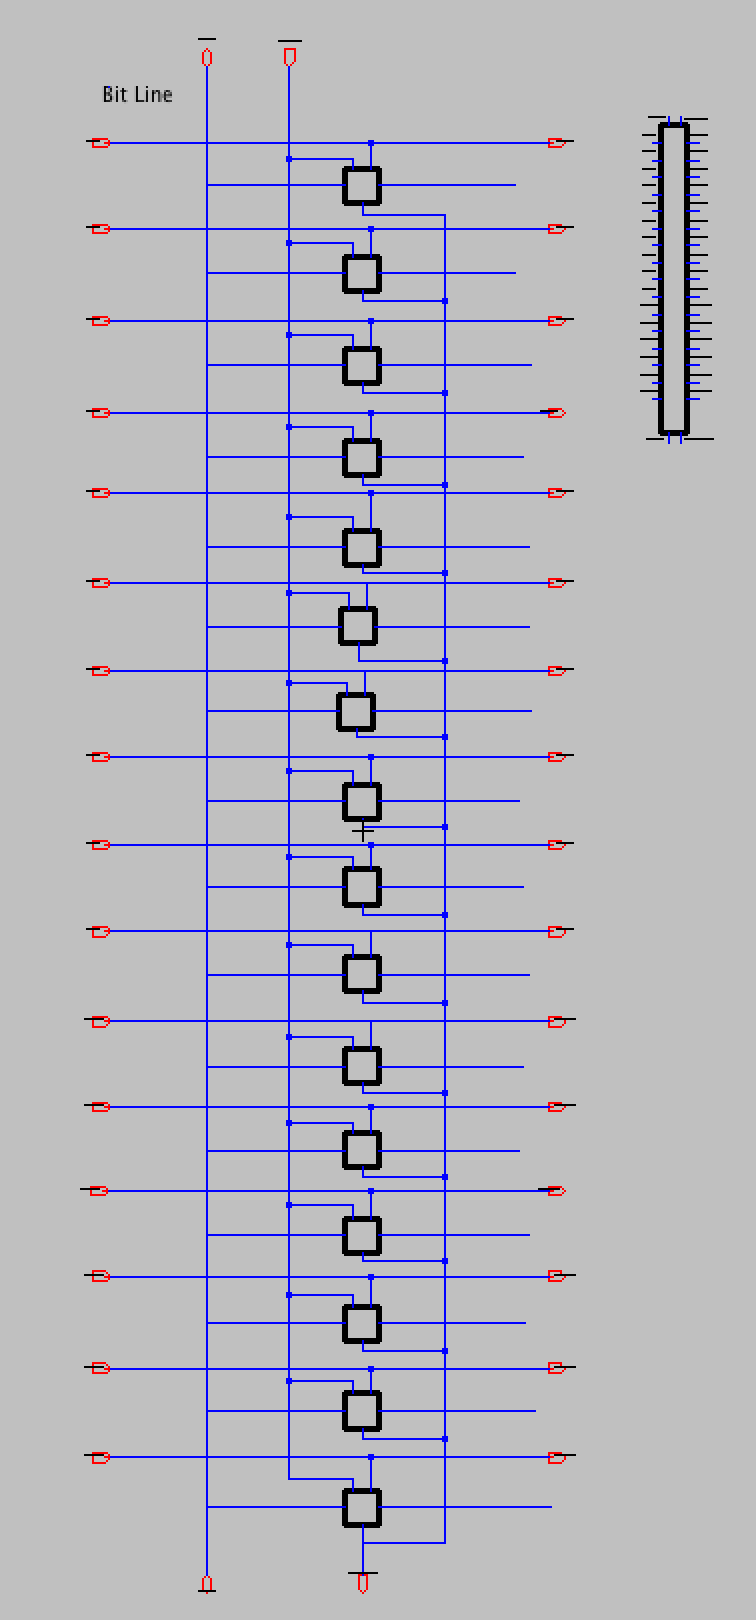
\includegraphics[scale=0.8]{bitLineSchematicZoomedOut}
	\caption{Entire Compiled Bitline}
	\label{fig:bitlineLongSchematic1}
\end{figure}

\begin{figure}[H]
	\centering
	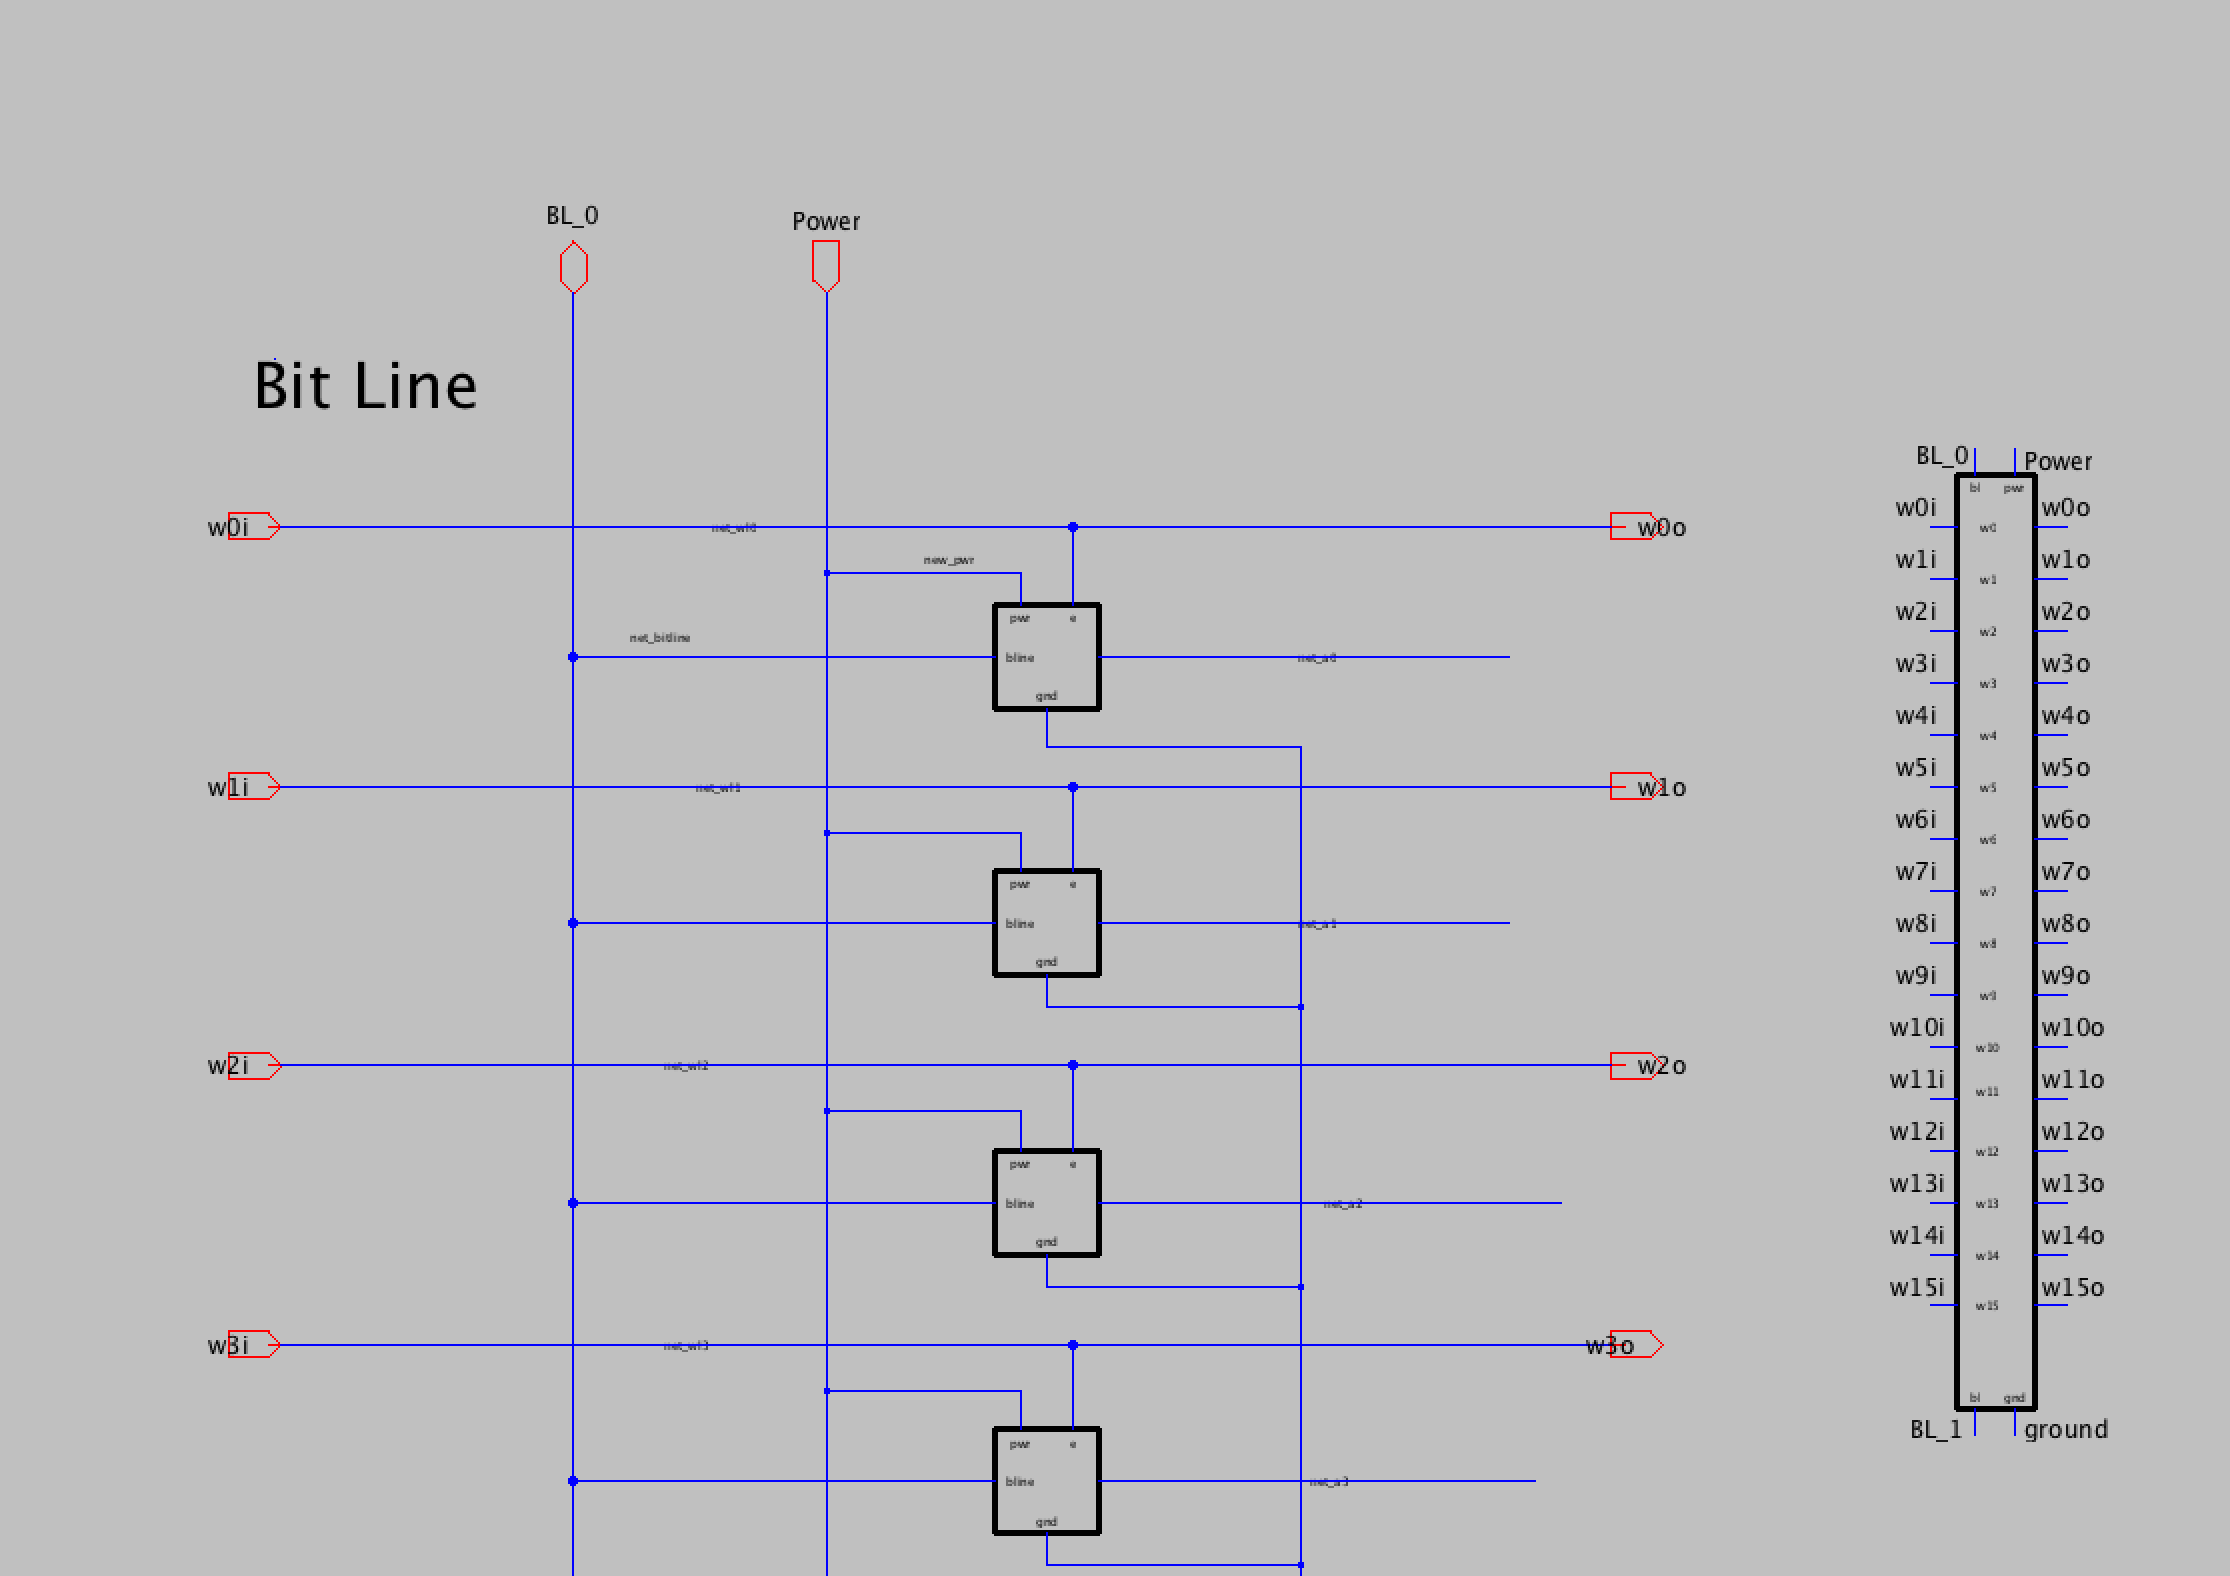
\includegraphics[scale=0.3]{bitLineSchematicZoomedIn}
	\caption{Entire Compiled Bitline Zommed In}
	\label{fig:bitlineLongSchematic2}
\end{figure}


\subsubsection{16x16 SRAM}
\label{sec:16x16_sram_design}
The 16x16 RAM is a collection of bit lines, sense amplifiers, bit line drivers, and $\frac{Vdd}{2}$ reference generators. The schematic for this 16x16 RAM is below in Figure \ref{fig:memory16x16Schematic}

\begin{figure}[H]
	\centering
	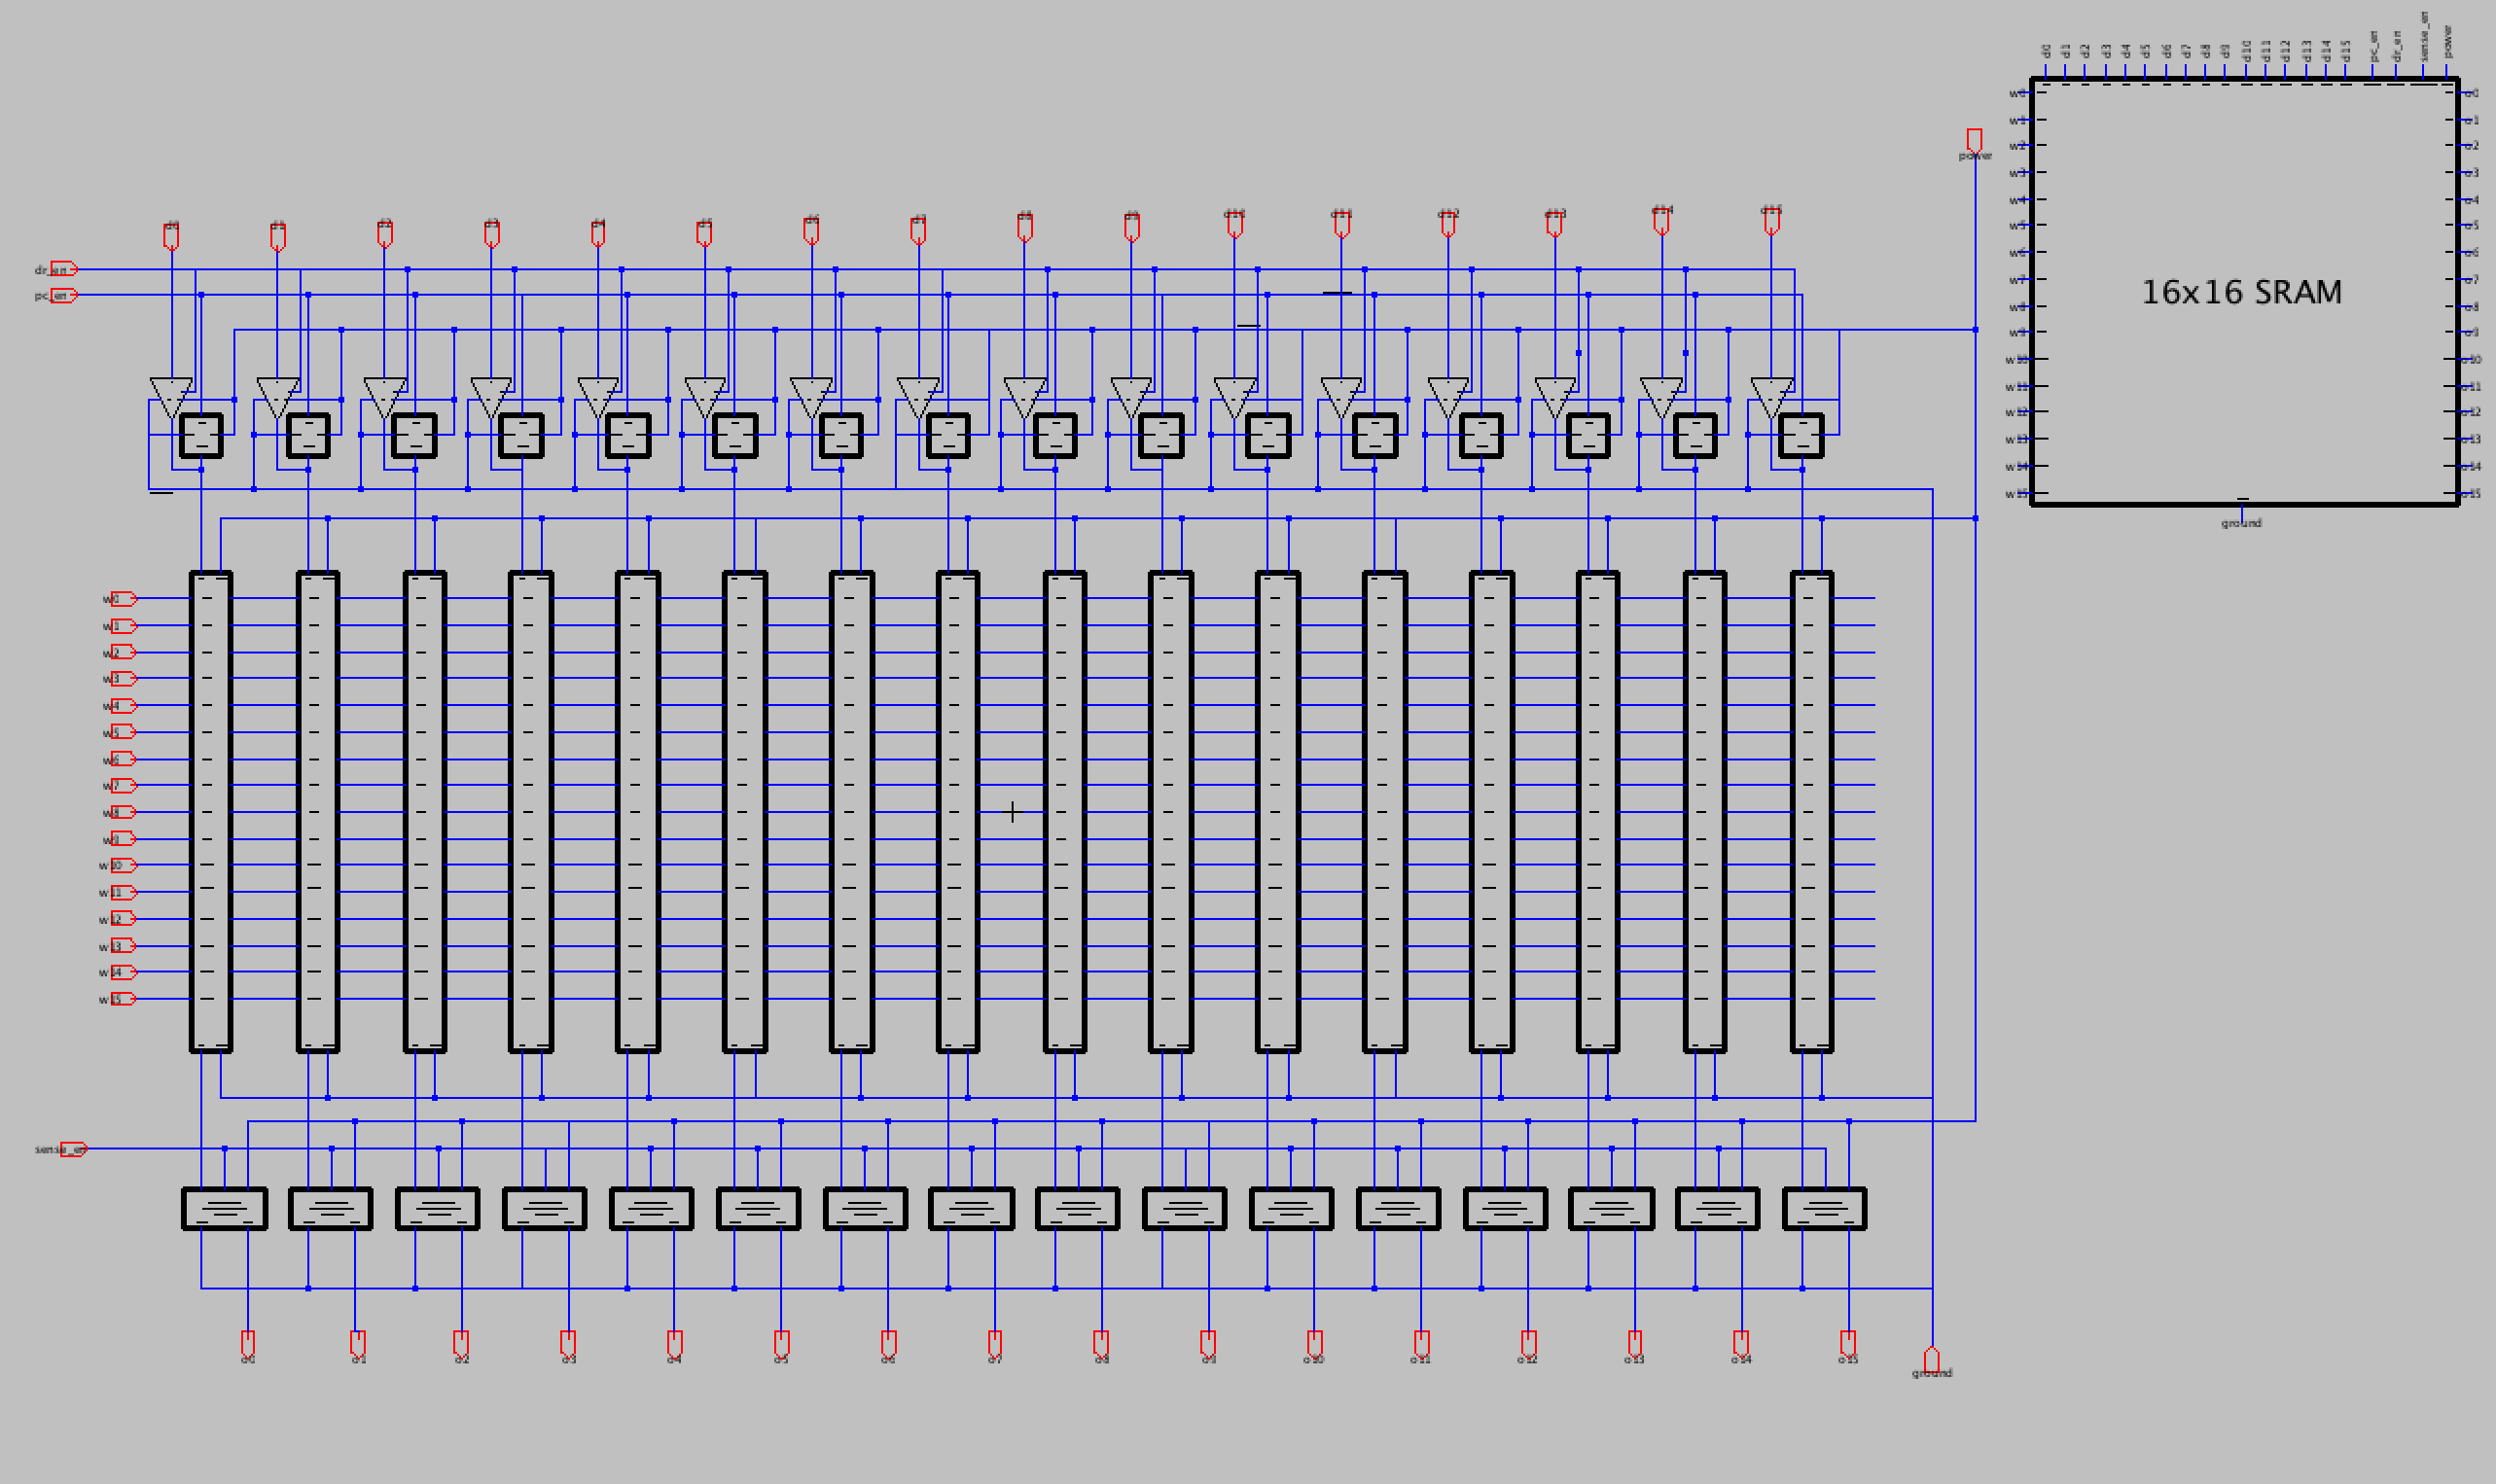
\includegraphics[scale=0.3]{memory16x16Schematic}
	\caption{16x16 RAM Schematic}
	\label{fig:memory16x16Schematic}
\end{figure}

Notice that the sense amplifier is a bit simplified from the one showed in Section \ref{sec:sense_amplifier}. This can be clearly seen in the zoomed shot in Figure \ref{fig:memory16x16SchematicSenseAmp}

\begin{figure}[H]
	\centering
	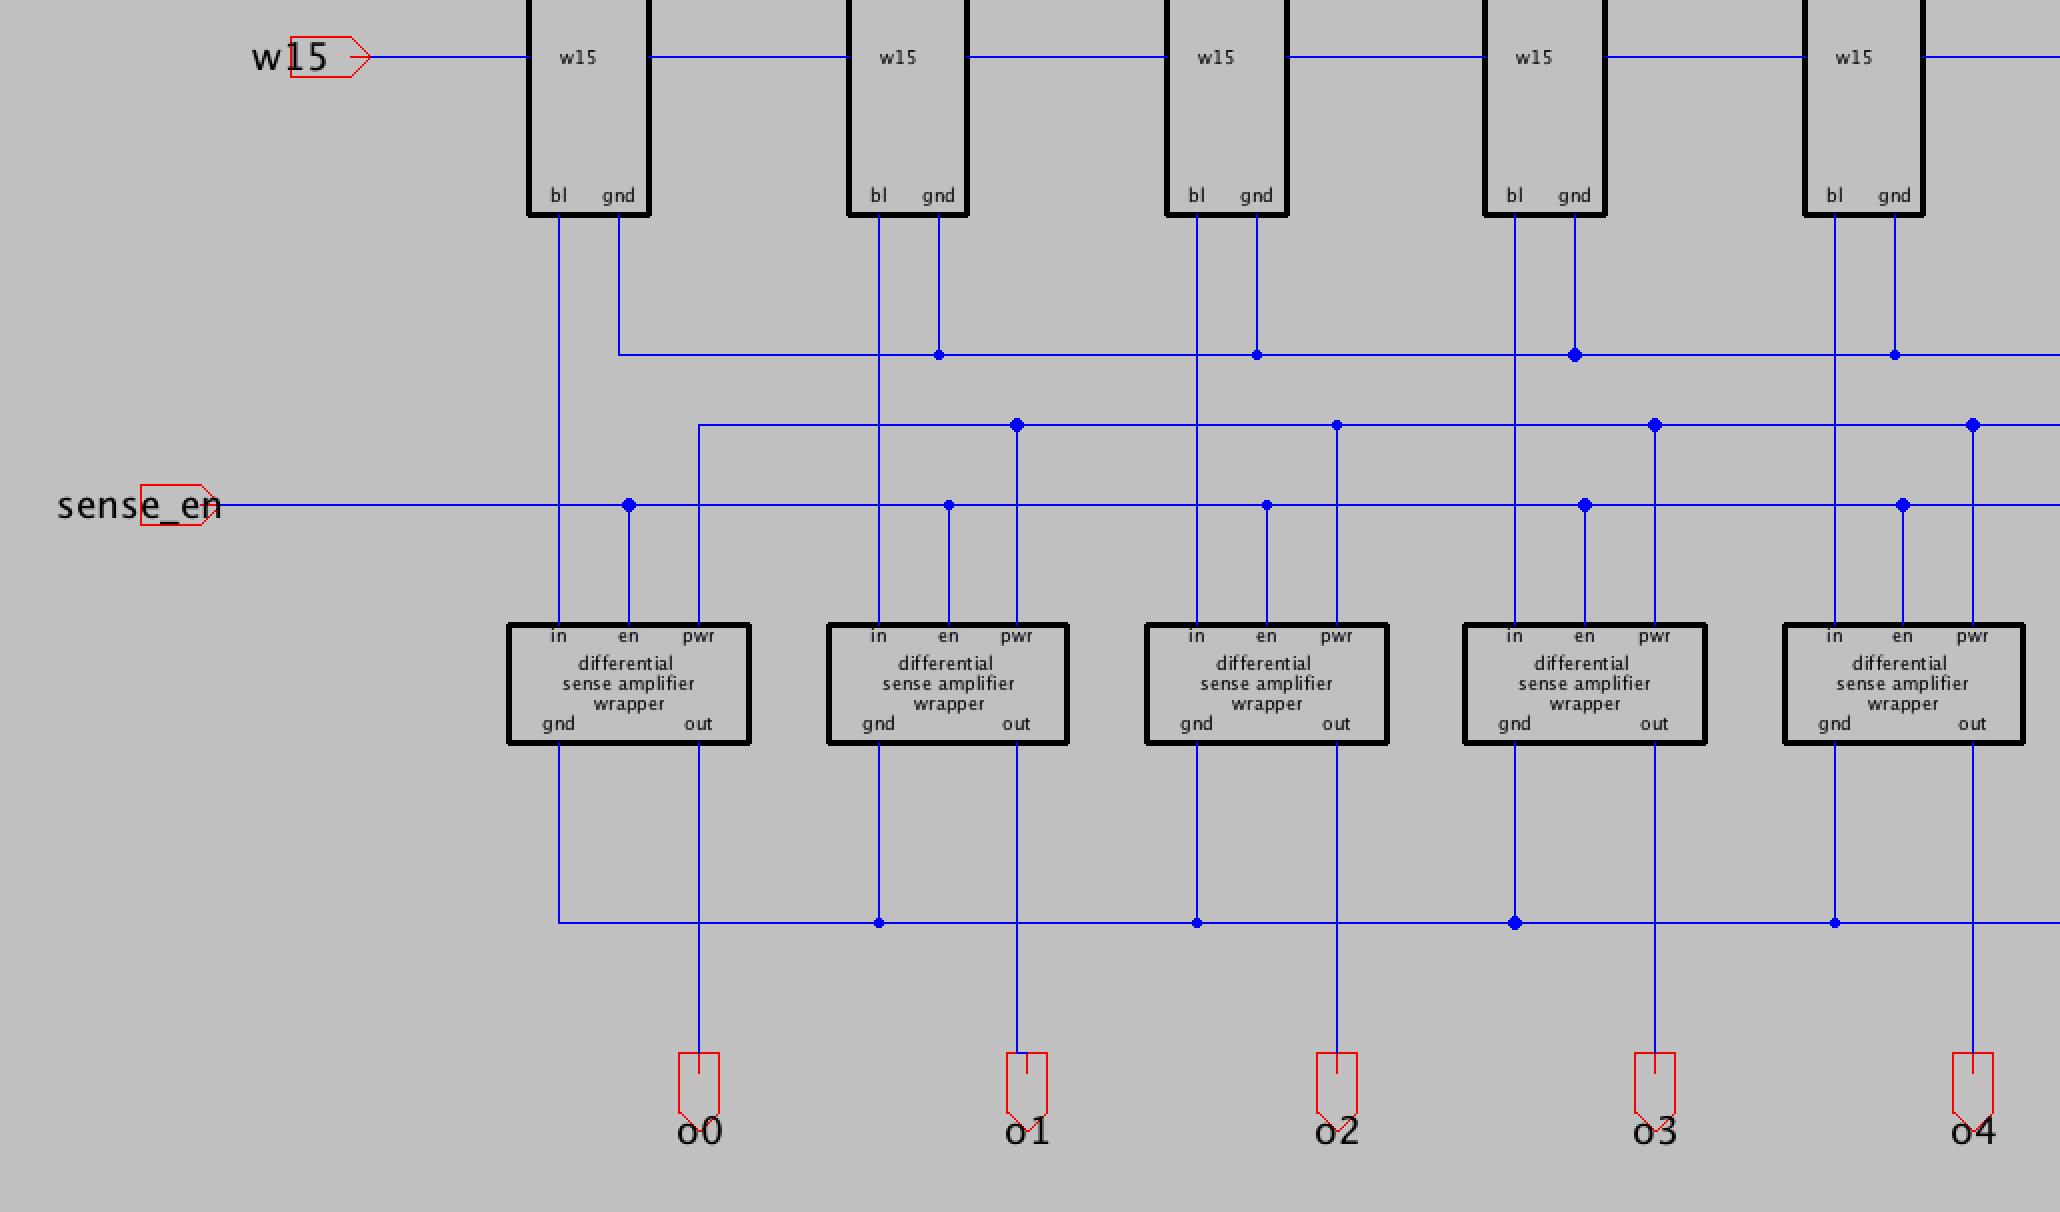
\includegraphics[scale=0.3]{memory16x16SchematicSenseAmp}
	\caption{16x16 RAM Zoomed In To Sense Amplifier}
	\label{fig:memory16x16SchematicSenseAmp}
\end{figure}

Here is the wrapper schematic:

\begin{figure}[H]
	\centering
	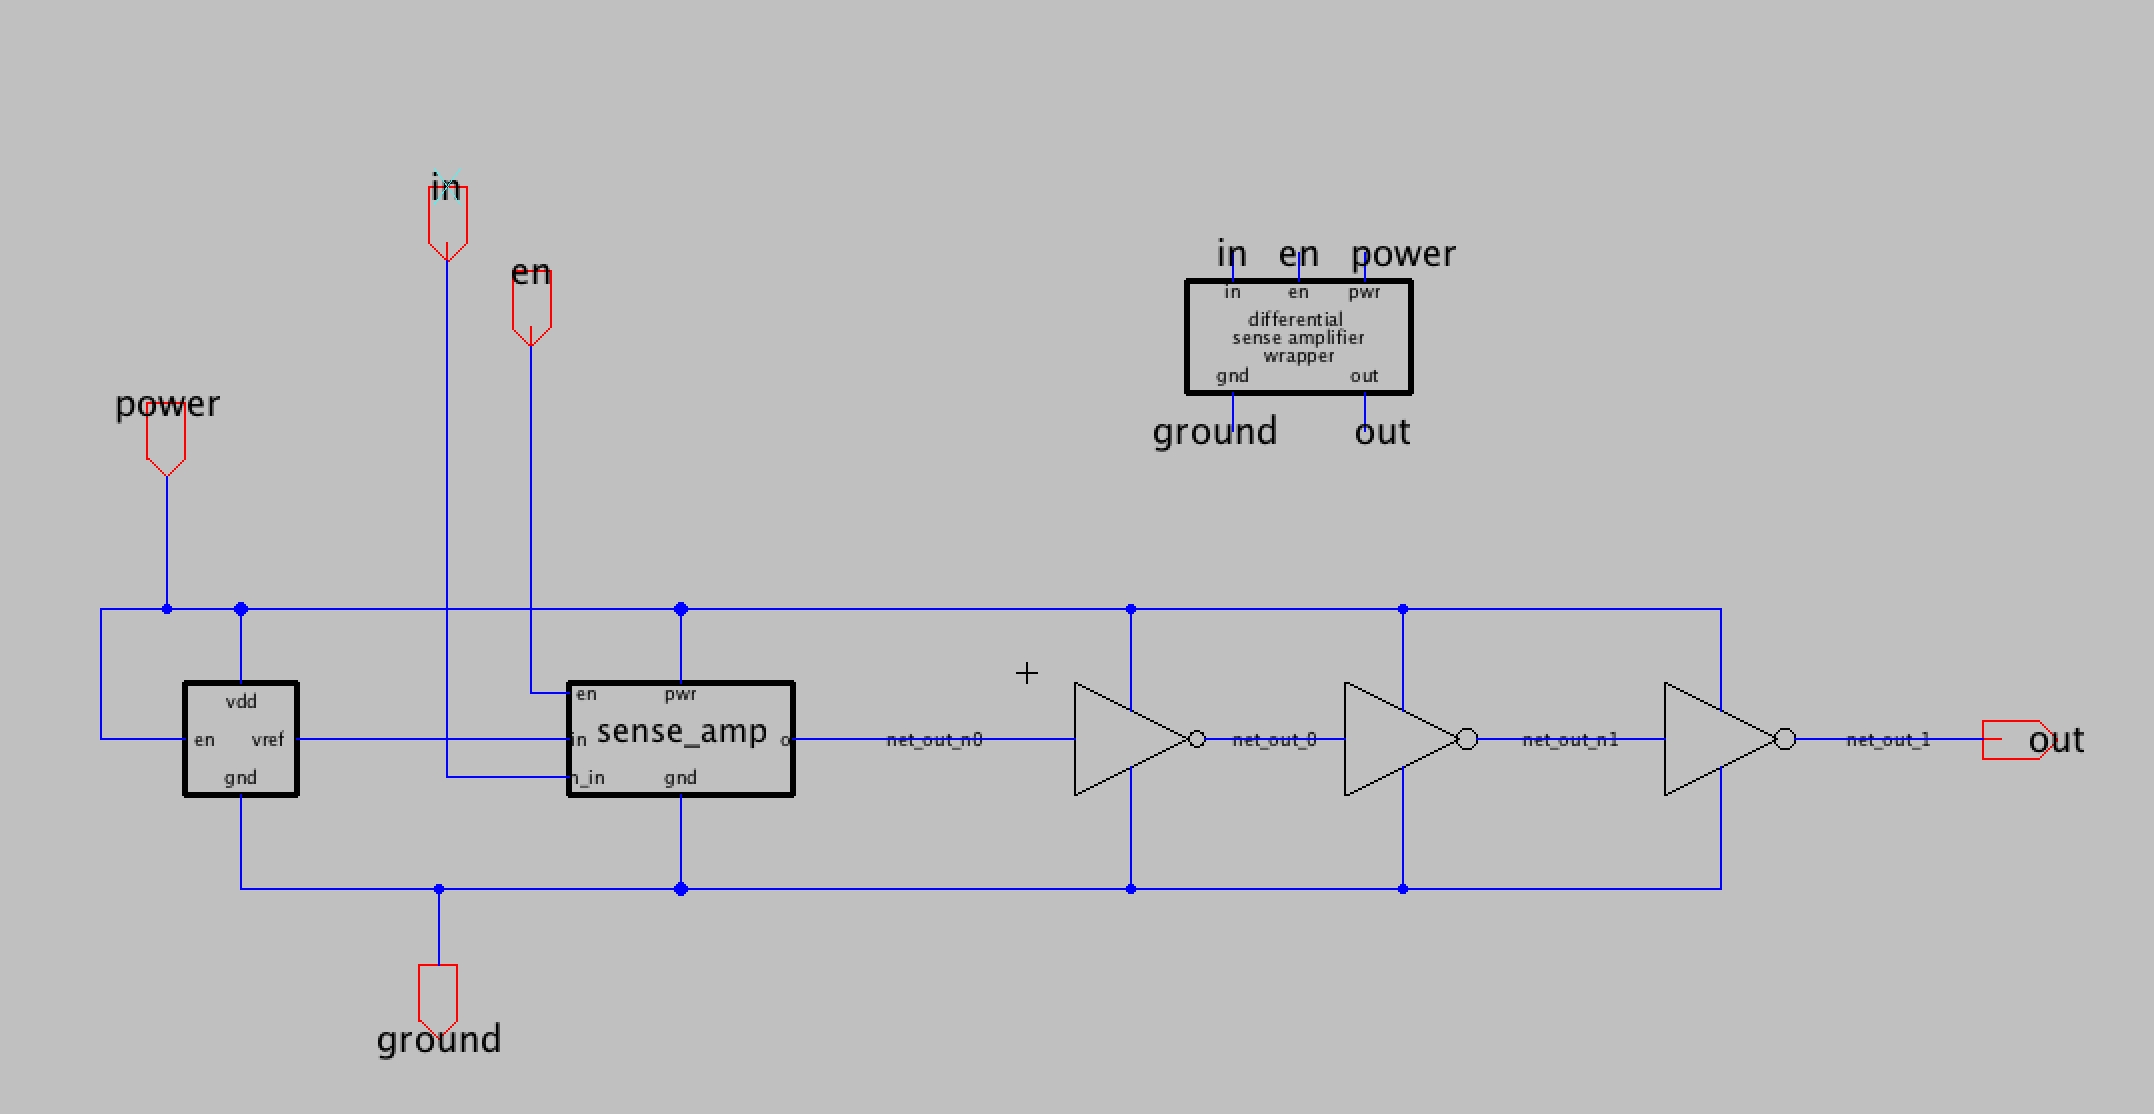
\includegraphics[scale=0.3]{senseAmpWrapperSch}
	\caption{Differential Sense Amplifier Wrapper Schematic}
	\label{fig:senseAmpWrapperSch}
\end{figure}

For the sake of completeness the details of the driver connections and pre-charge module can be seen in Figure \ref{fig:memory16x16SchematicDriver}.

\begin{figure}[H]
	\centering
	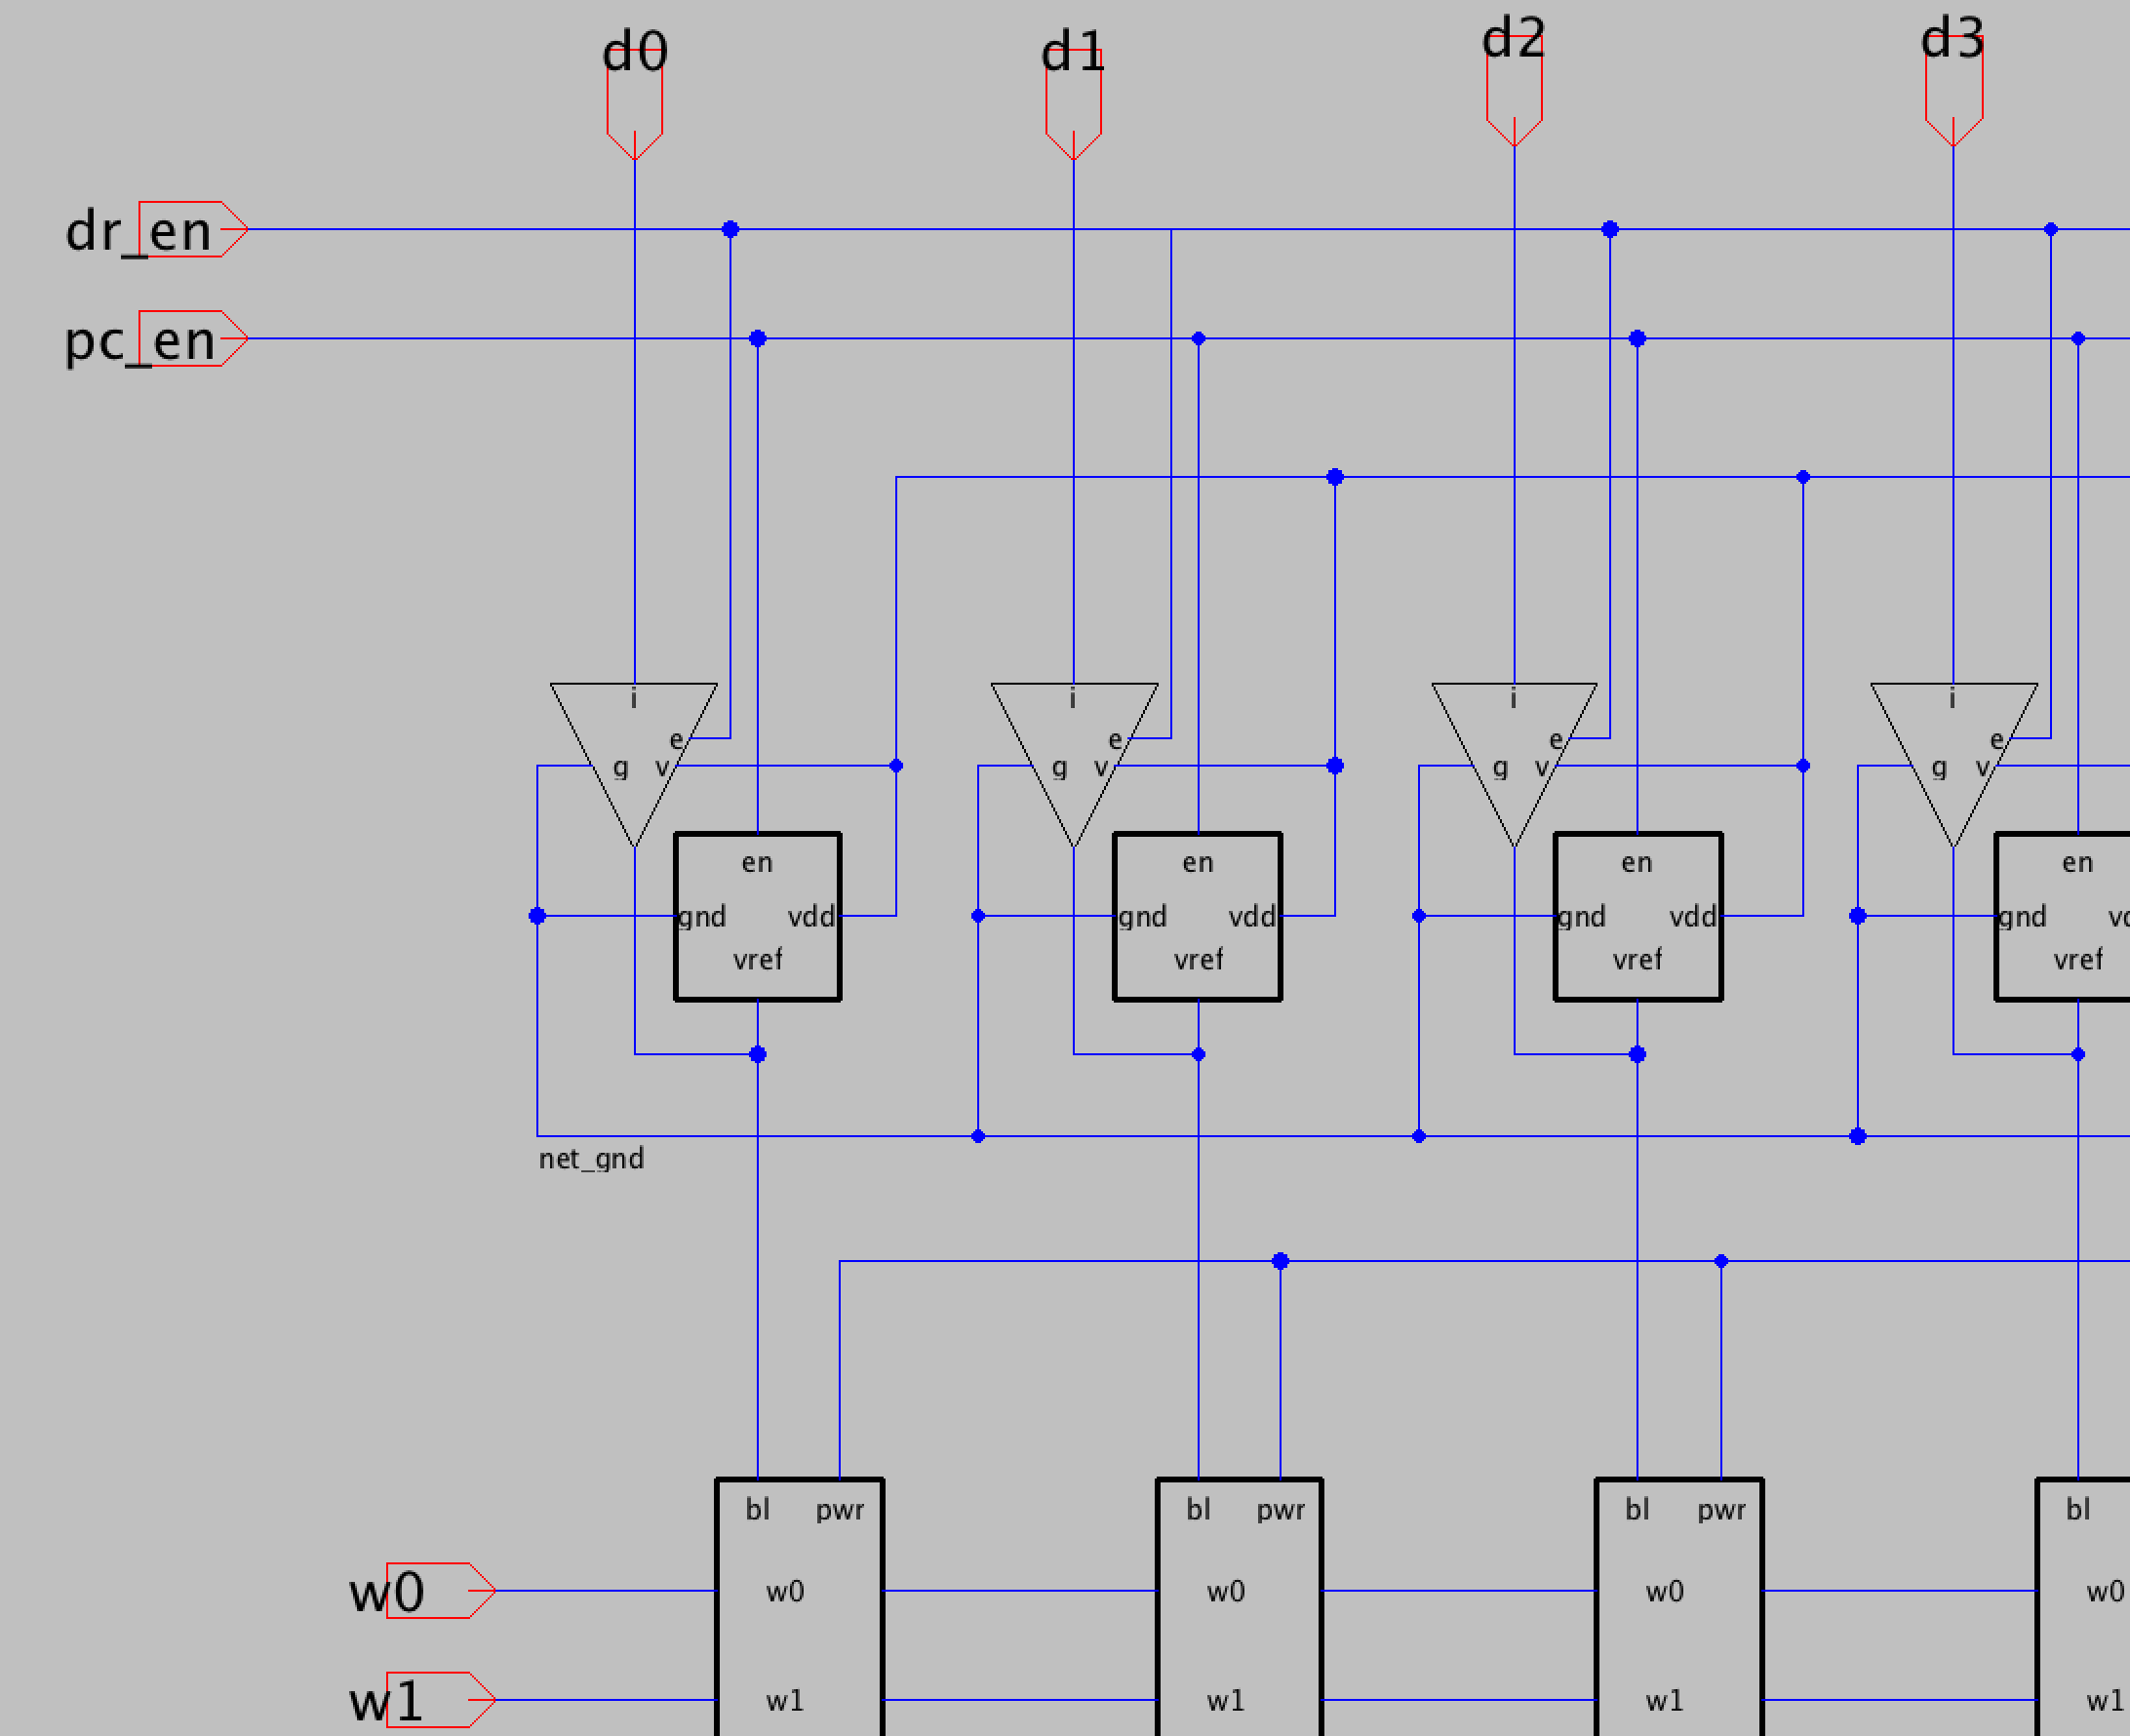
\includegraphics[scale=0.3]{memory16x16SchematicDriver}
	\caption{16x16 RAM Zoomed In To Driver and Pre-Charge Module}
	\label{fig:memory16x16SchematicDriver}
\end{figure}

\textbf{Correctness}\\
To test correctness of the 16x16 RAM, we used the decoder to select the address--the design of which is detailed in Section \ref{sec:decoder_design}. Then, we wrote to every address once and immediately read from every address twice. The entire test schematic is shown in Figure \ref{fig:memory16x16TestSchematic}.

\begin{figure}[H]
	\centering
	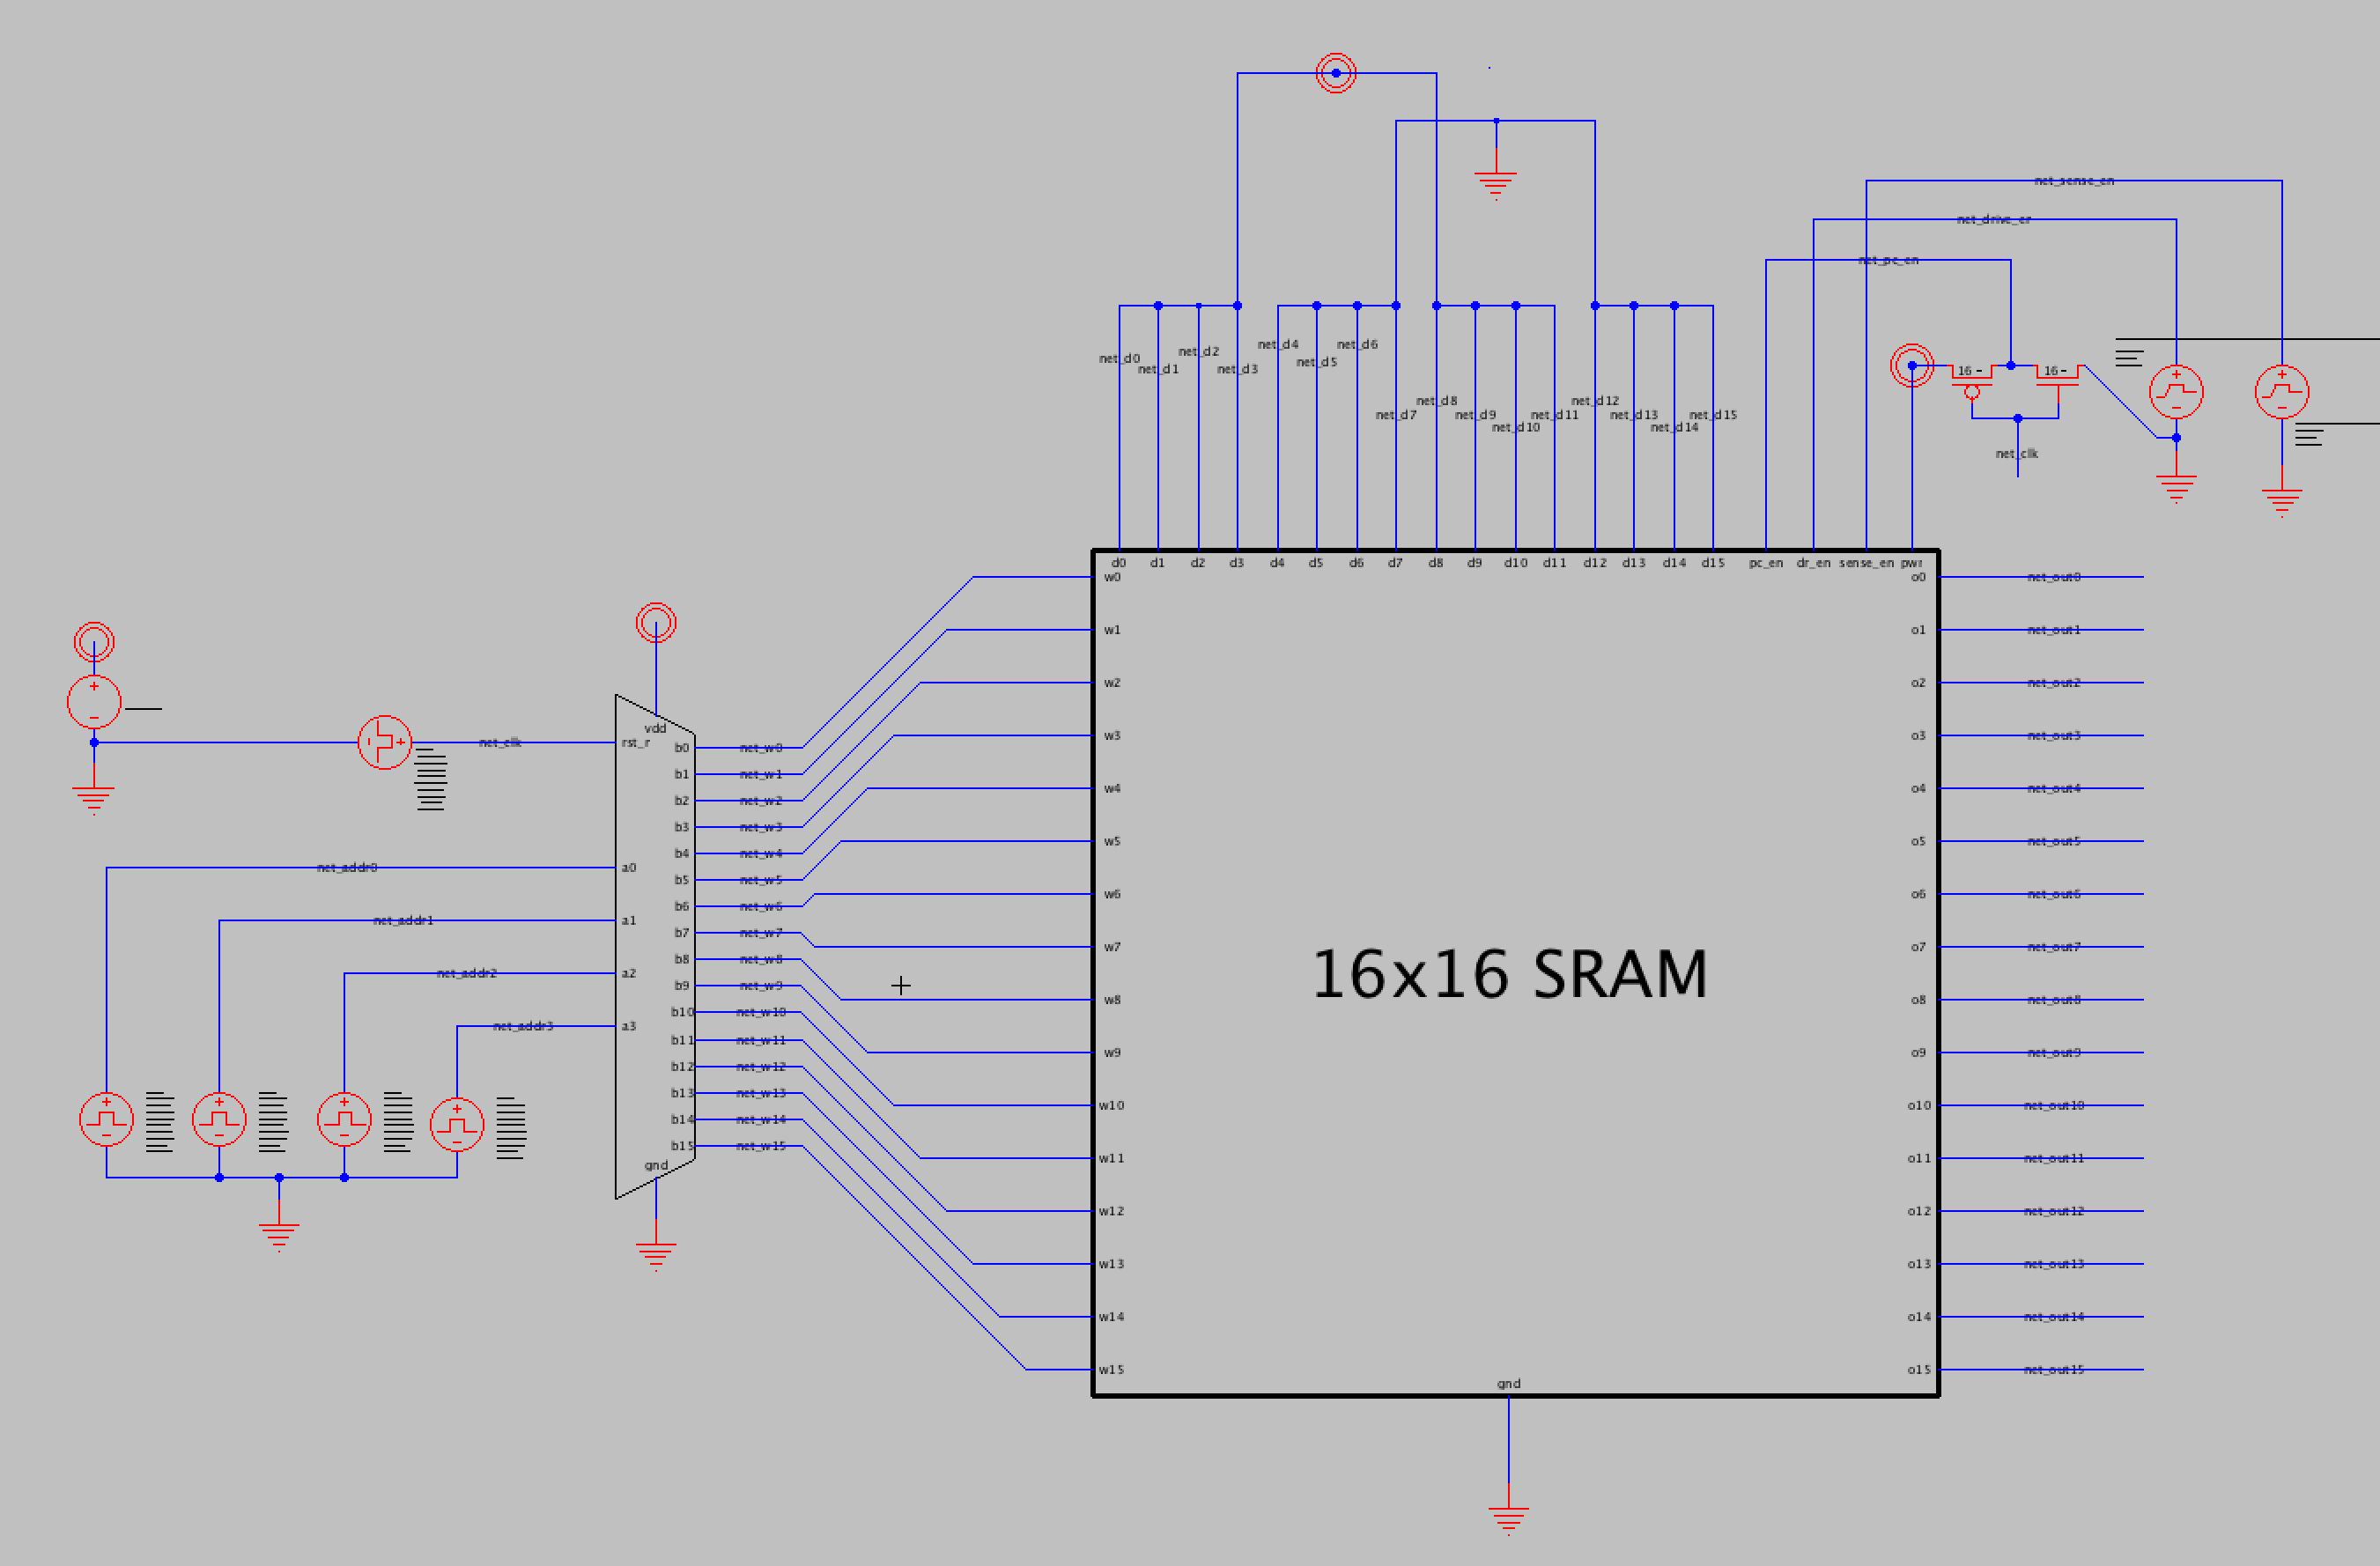
\includegraphics[scale=0.3]{memory16x16TestSchematic}
	\caption{16x16 RAM Test Schematic}
	\label{fig:memory16x16TestSchematic}
\end{figure}

To drive the wordlines, we used the aforementioned decoder and 4 $VV\_Pulse$s. The wordline is driven low via a $rst\_n$ signal. A single pulse is high for long enough to complete 1 write operation and 2 read operations at 1Ghz per operation.

\begin{figure}[H]
	\centering
	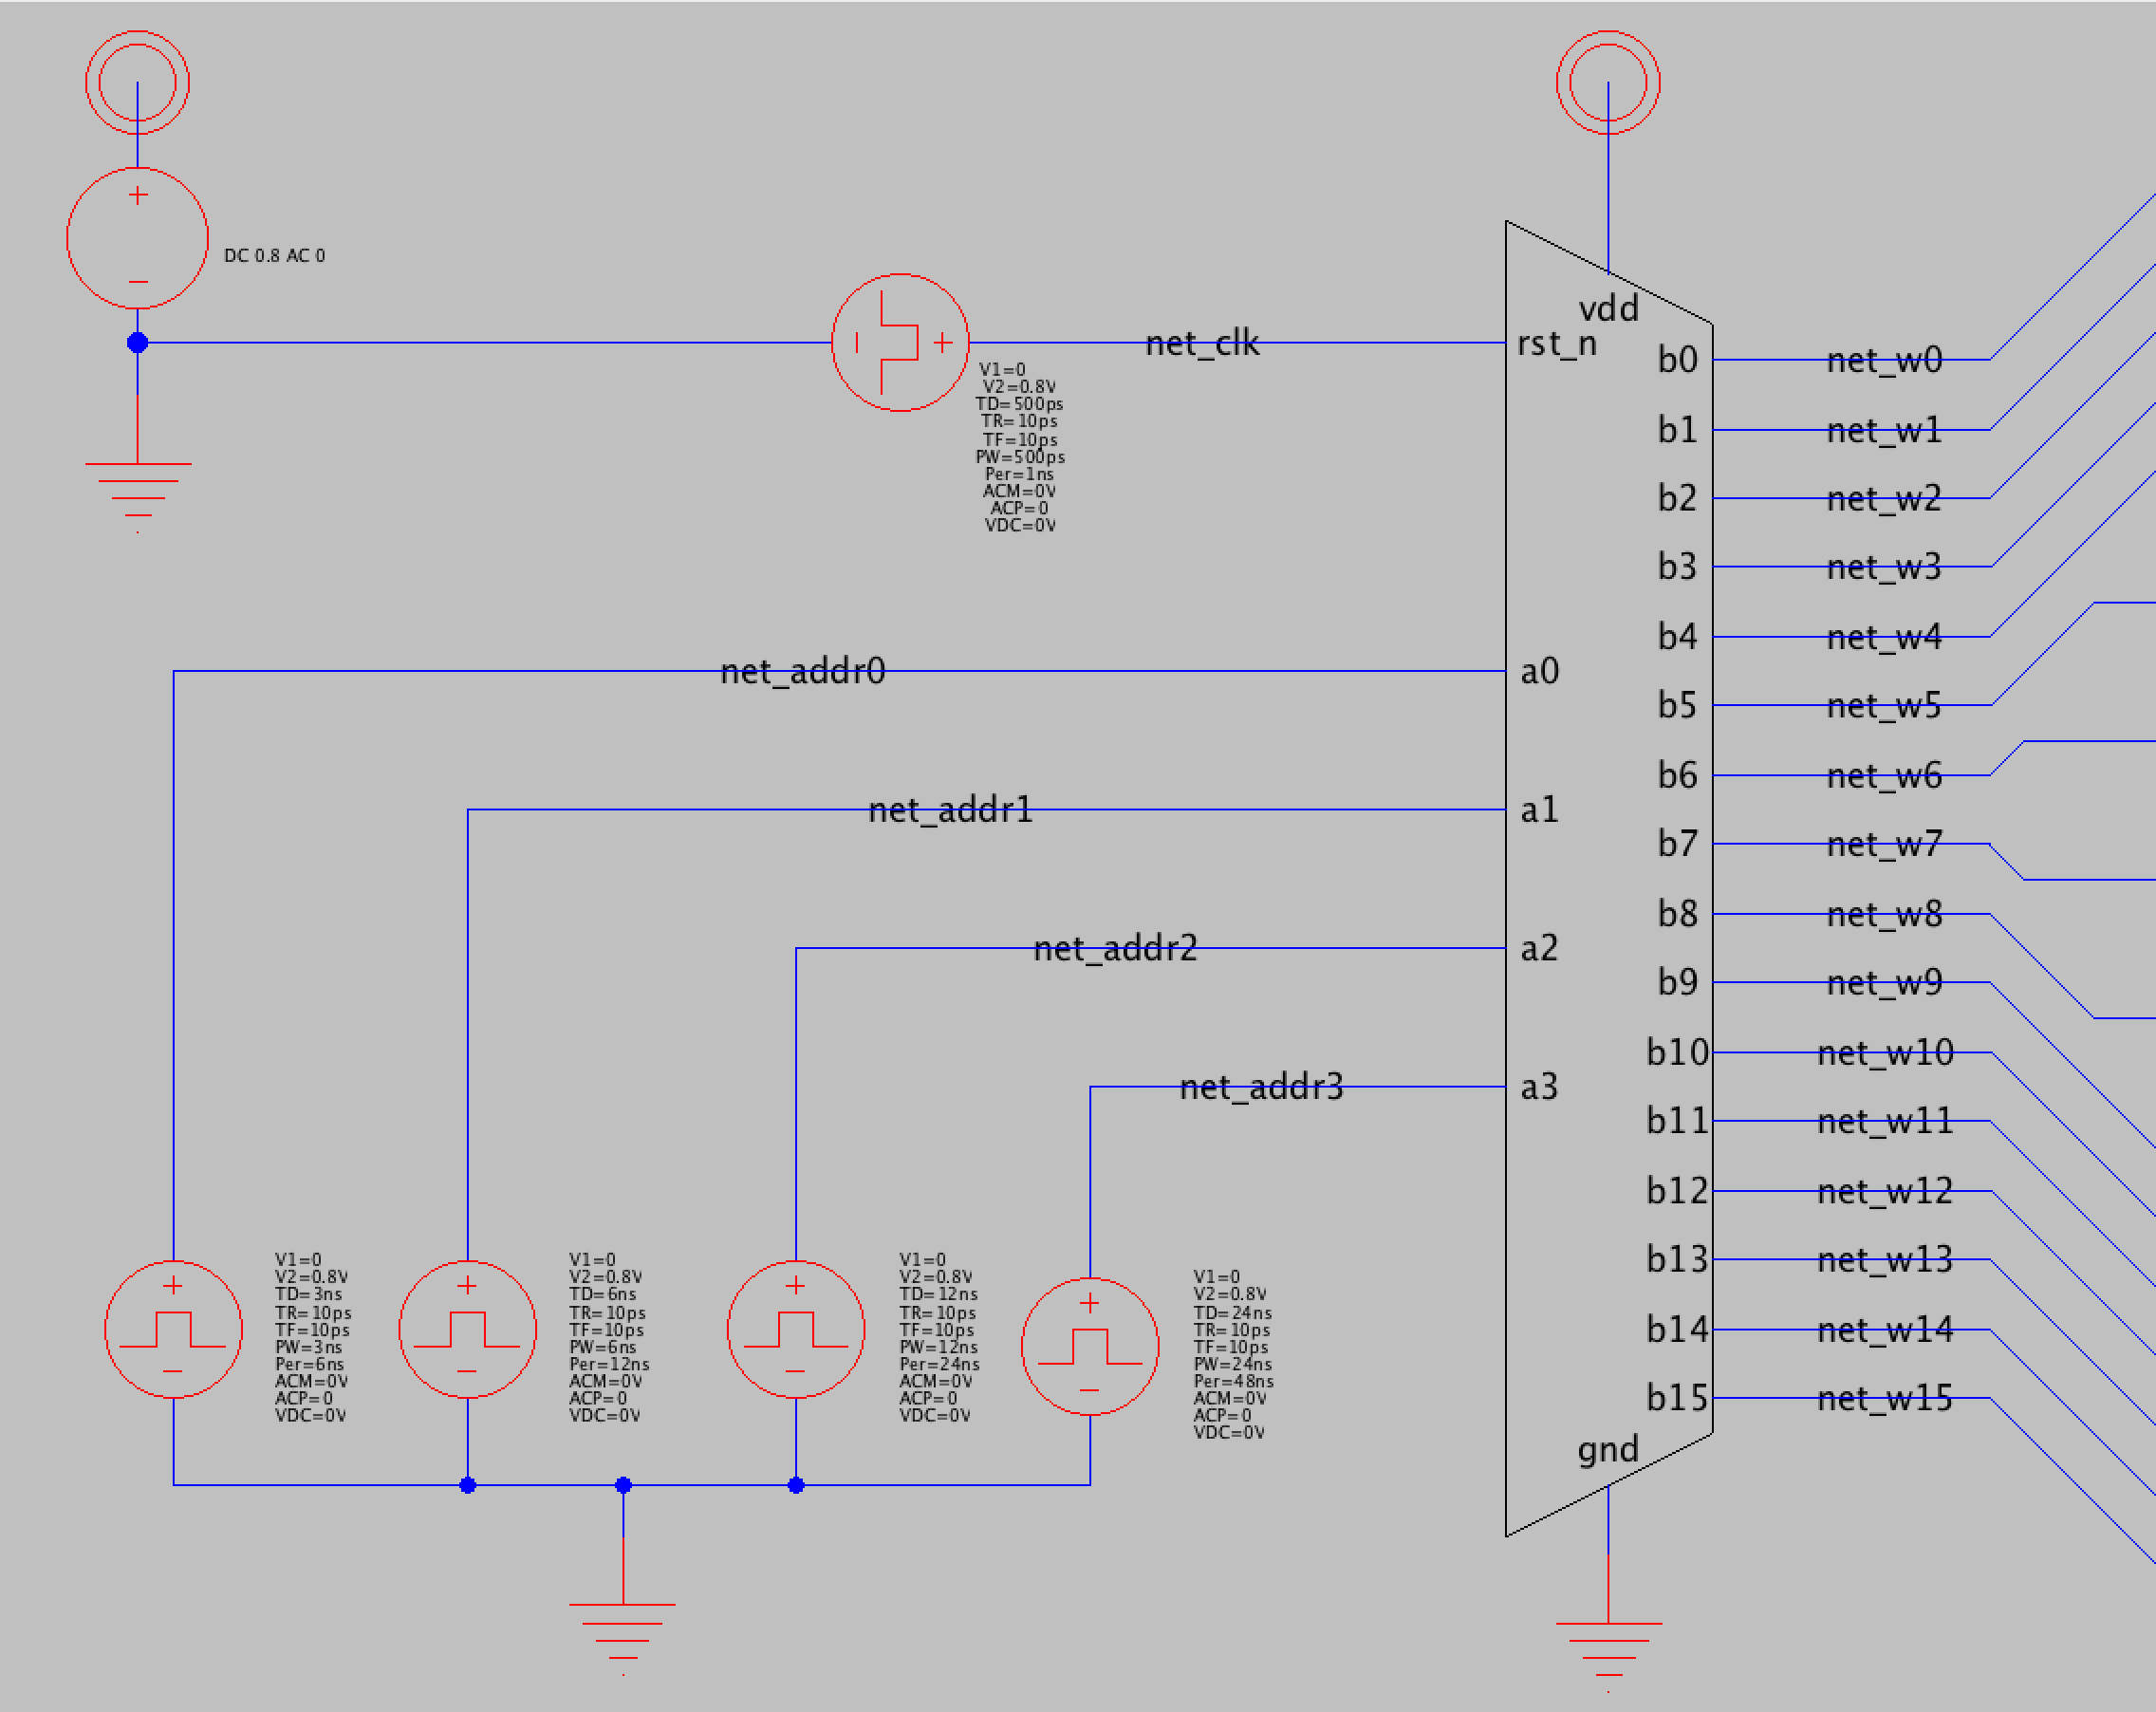
\includegraphics[scale=0.3]{memory16x16TestSchematicWordlines}
	\caption{16x16 RAM Test Zoomed to Wordlines}
	\label{fig:memory16x16TestSchematicWordlines}
\end{figure}

Here is the waveform for the wordline inputs:

\begin{figure}[H]
	\centering
	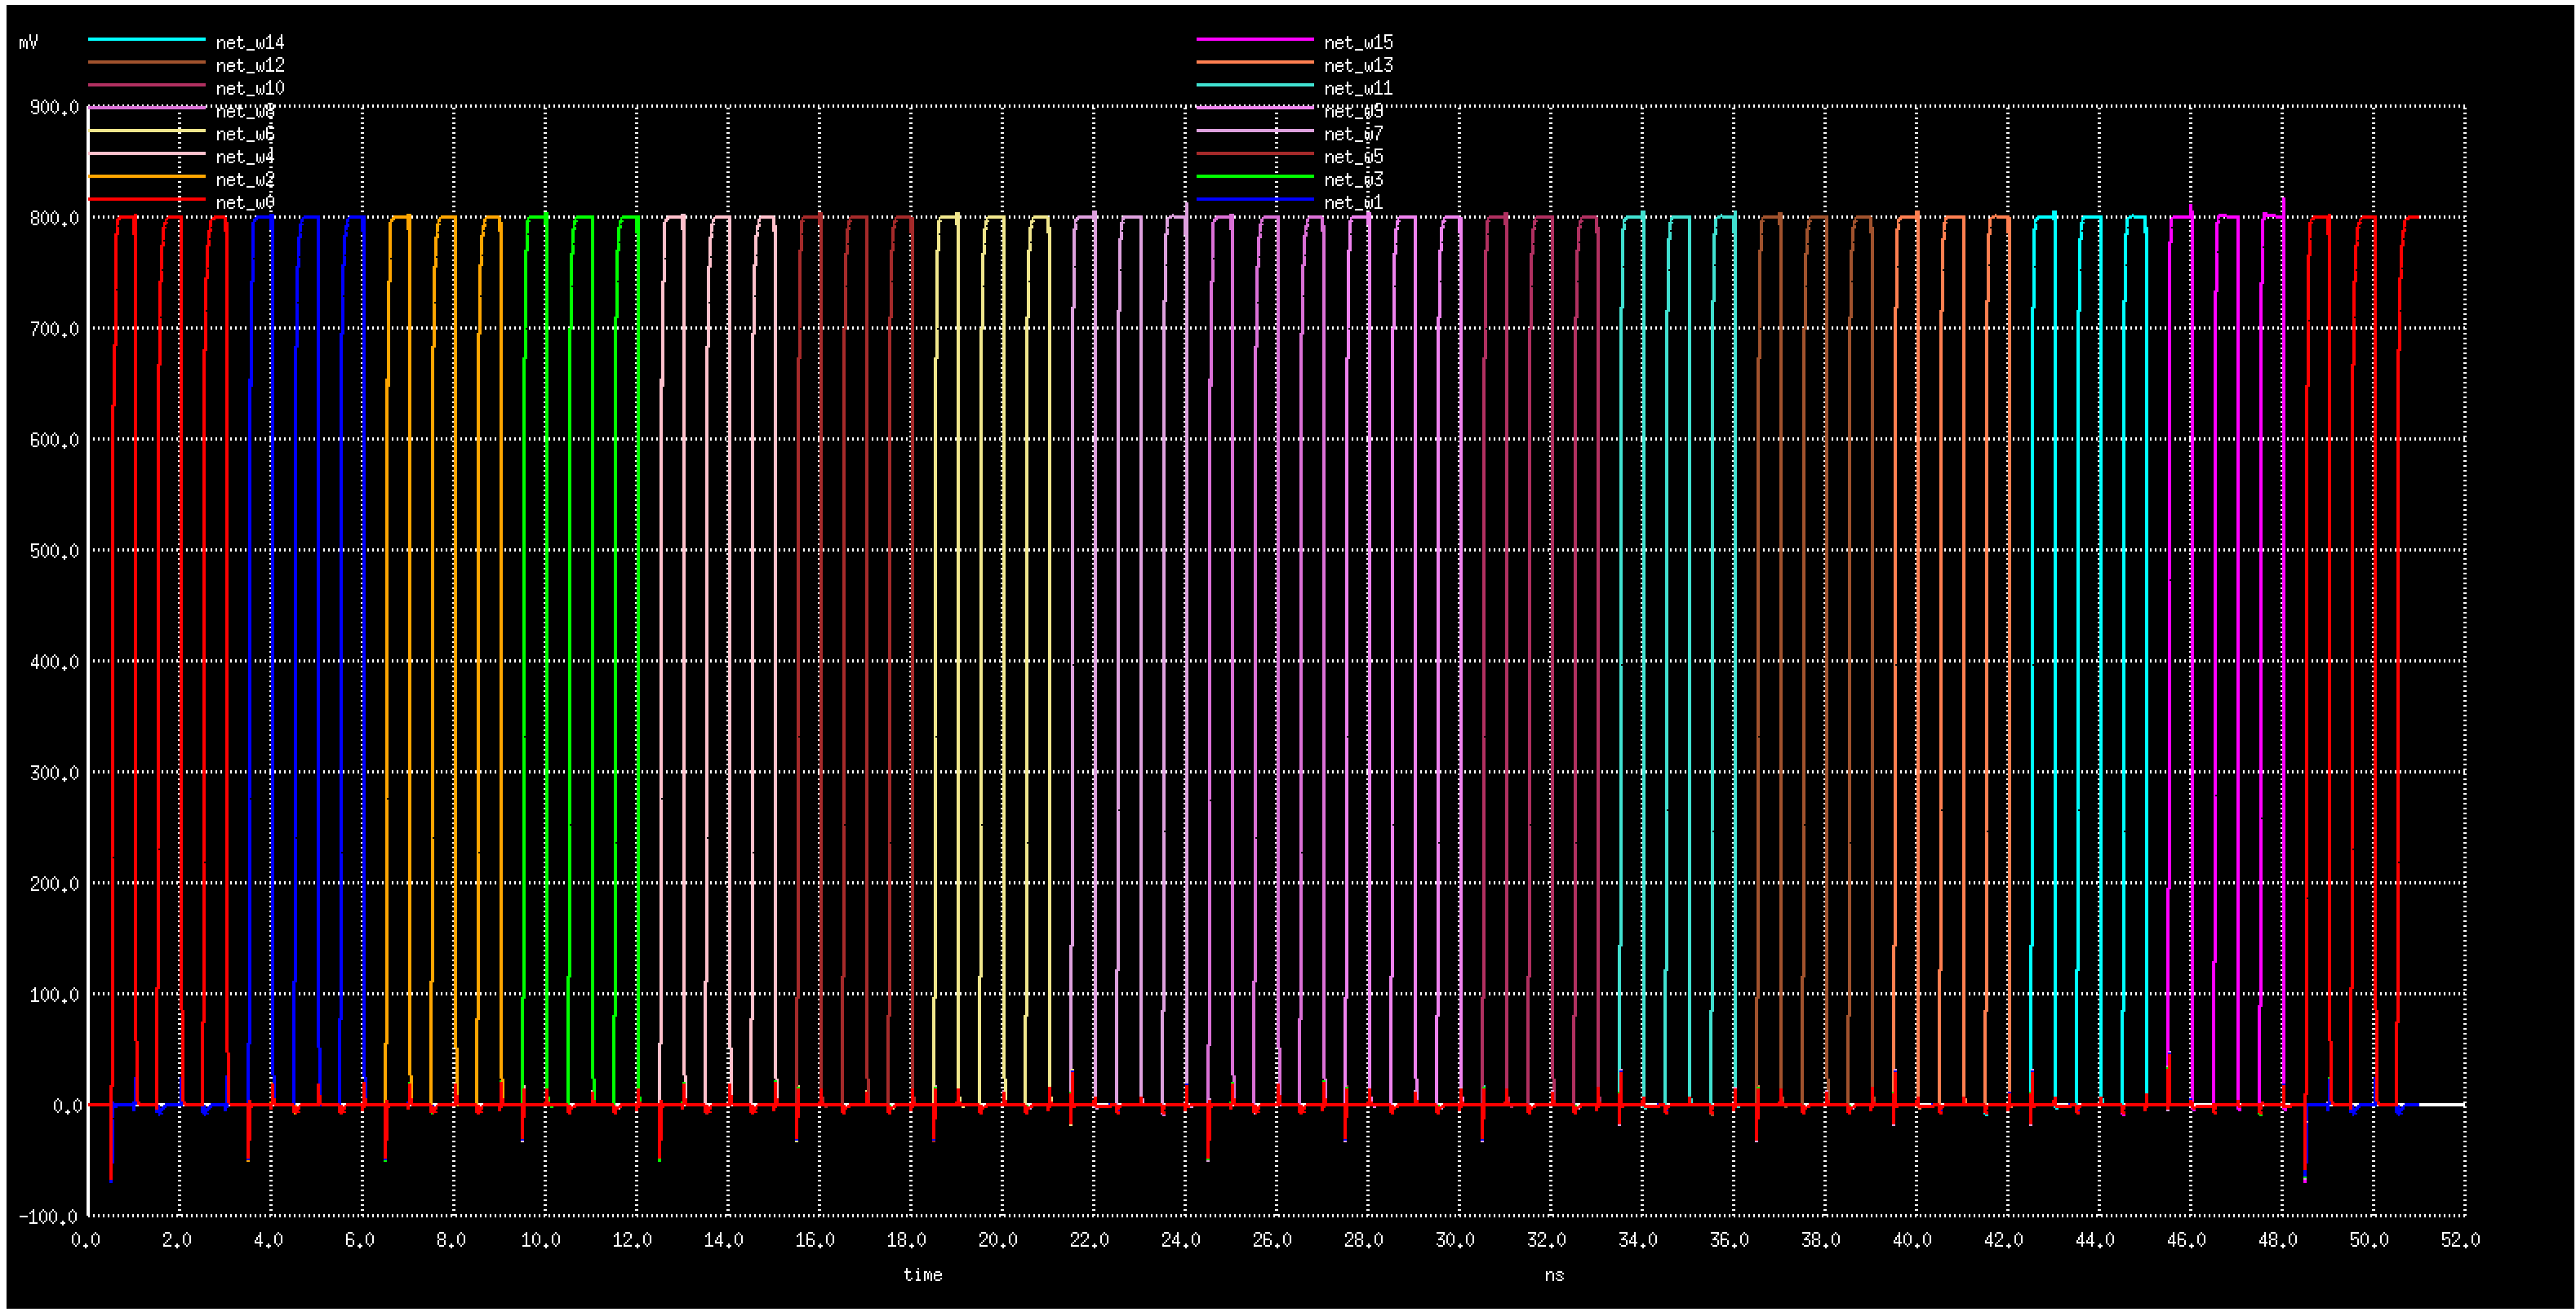
\includegraphics[scale=0.25]{memory16x16TestWaveformWordline}
	\caption{16x16 RAM Test Wordline Waveform}
	\label{fig:memory16x16TestWaveformWordline}
\end{figure}

The data that is placed in each wordline is the 4 bit address distributed across the 16 bit input. This is so we can guarantee that writing different data in each cell does not override another cell. See Figure \ref{fig:memory16x16TestSchematicDataLines} below:

\begin{figure}[H]
	\centering
	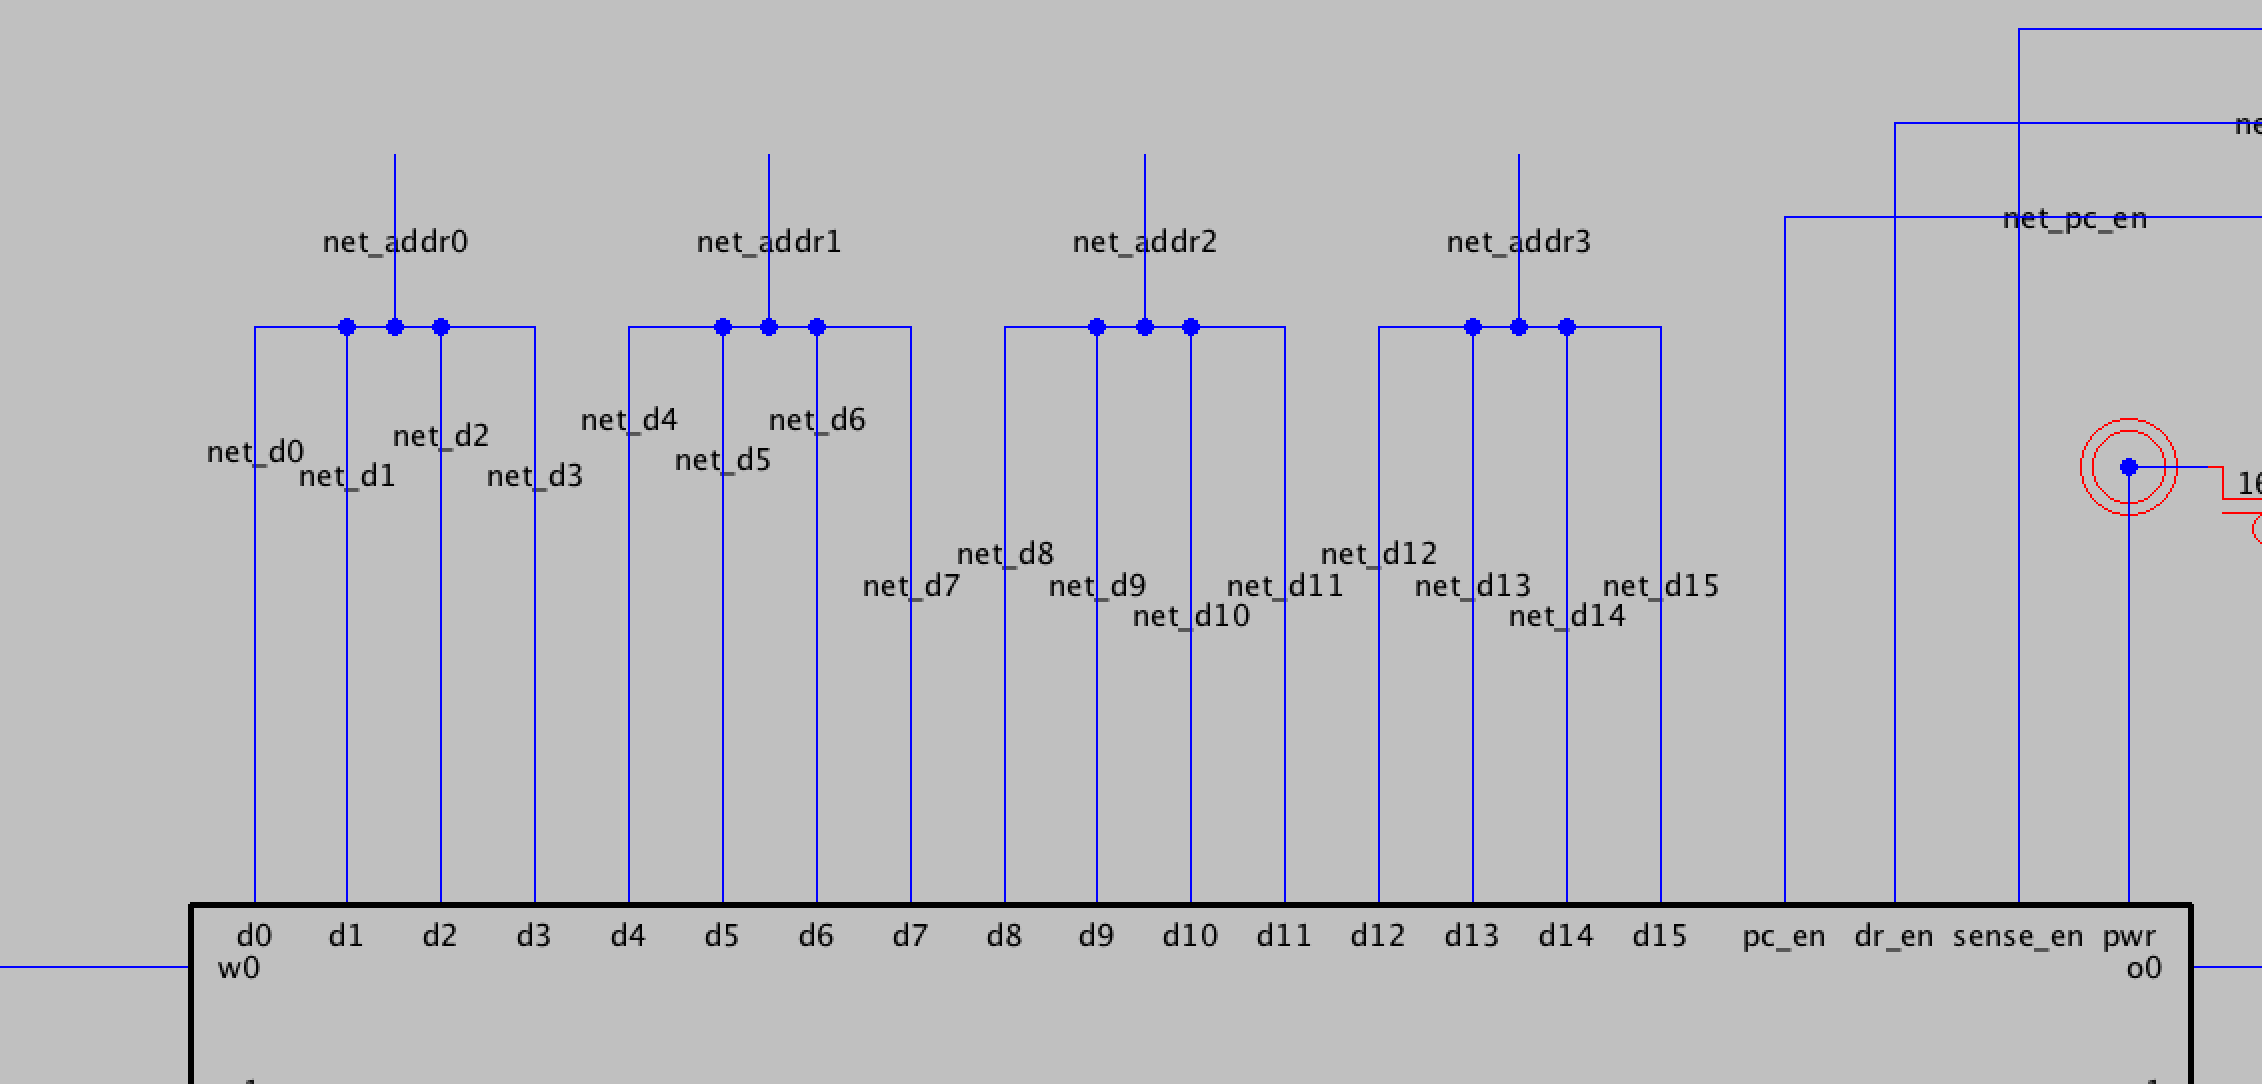
\includegraphics[scale=0.3]{memory16x16TestSchematicDataLines}
	\caption{16x16 RAM Test Zoomed to Data Input}
	\label{fig:memory16x16TestSchematicDataLines}
\end{figure}

Here are the output waveforms with their corresponding input address bit (Figure \ref{fig:memory16x16TestWaveformOutputCorrectness}). Notice that each output has two pulses--this is for the two reads that we do of each address. 

\begin{figure}[H]
	\centering
	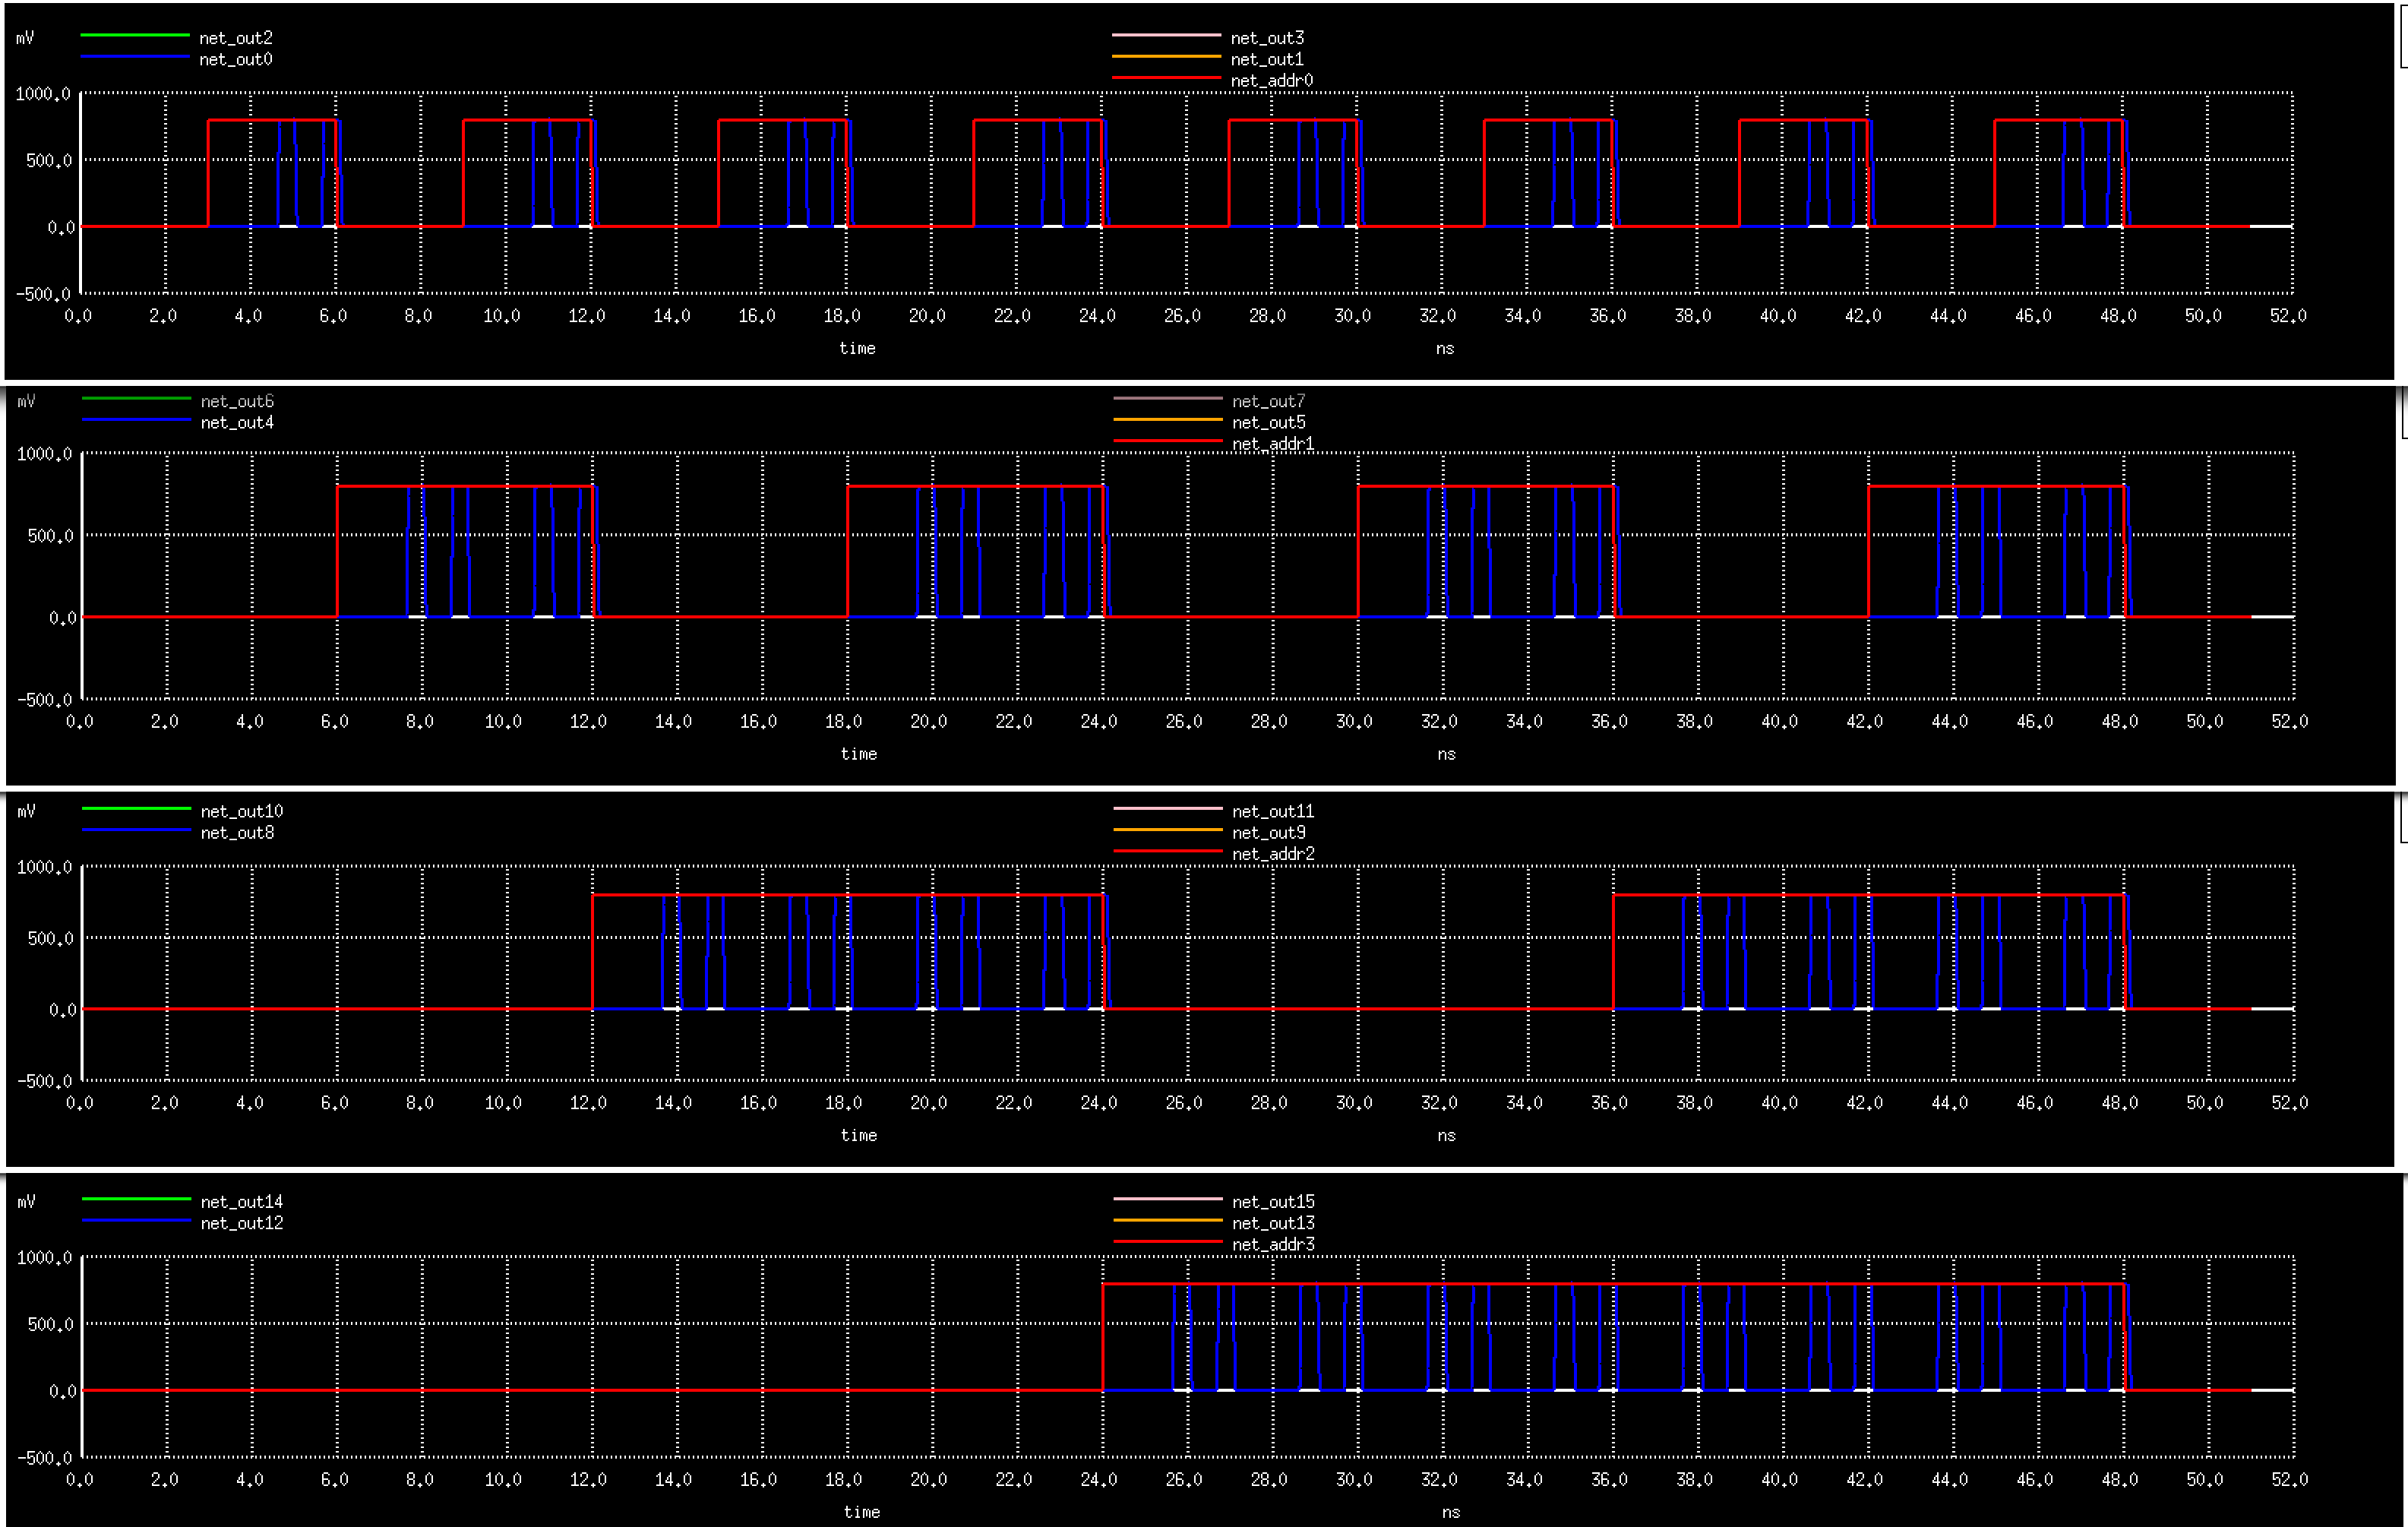
\includegraphics[scale=0.2]{memory16x16TestWaveformOutputCorrectness}
	\caption{16x16 RAM Test Output with Corresponding Address Bit}
	\label{fig:memory16x16TestWaveformOutputCorrectness}
\end{figure}
\newpage
Finally, we have the control inputs of $net\_sense\_en$, $net\_pc\_en$, and $net\_drive\_en$.

\begin{figure}[H]
	\centering
	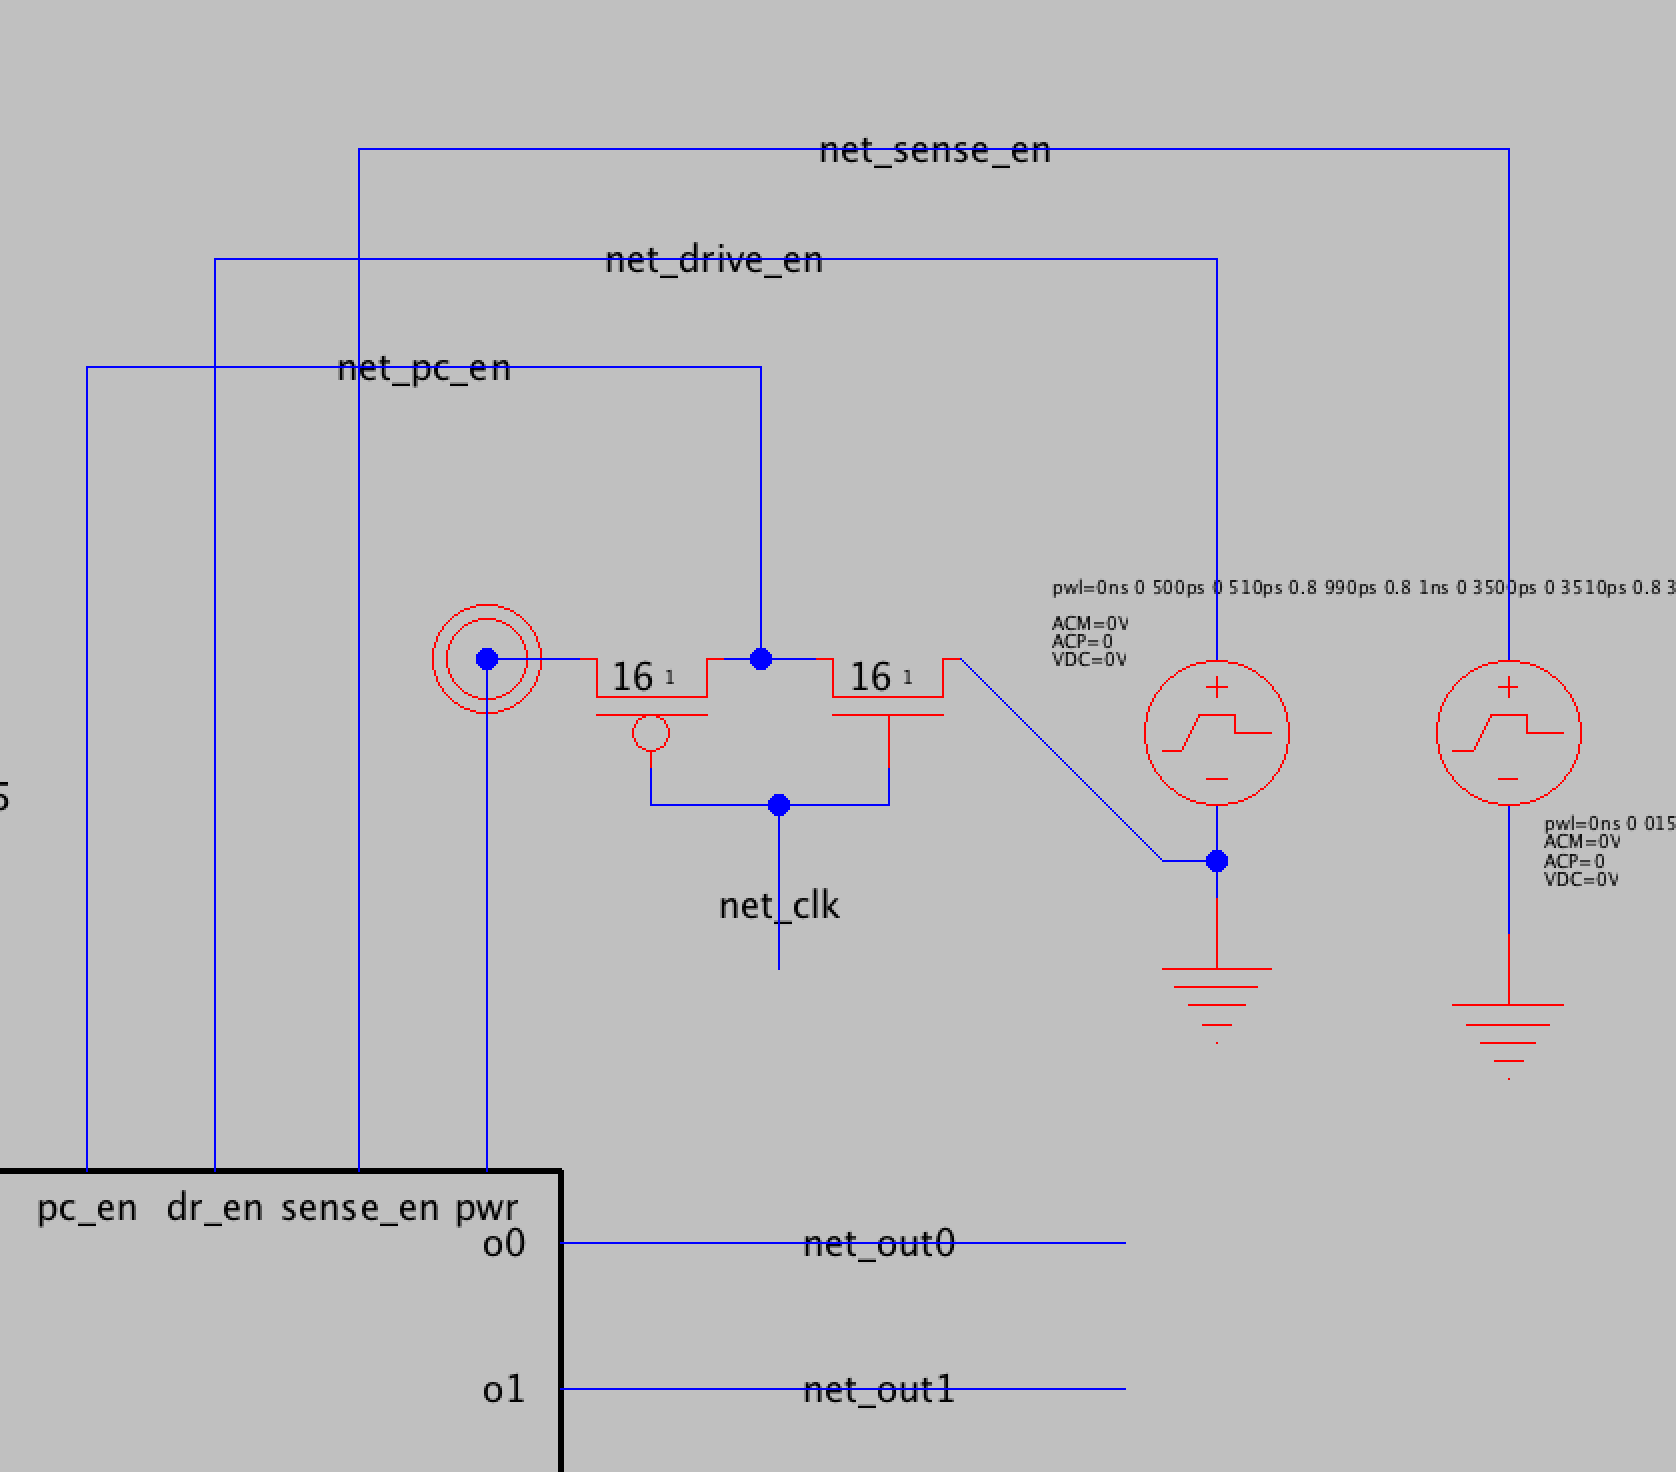
\includegraphics[scale=0.35]{memory16x16TestSchematicControl}
	\caption{16x16 RAM Test Zoomed to Data Input}
	\label{fig:memory16x16TestSchematicControl}
\end{figure}

\newpage
Since the pulse data goes off the page, here is the information for $net\_sense\_en$:\\\\
\code {
0ns 0\\
01510ps 0 01520ps 0.8 01950ps 0.8 02ns 0\\
02510ps 0 02520ps 0.8 02990ps 0.8 03ns 0\\
04510ps 0 04520ps 0.8 04950ps 0.8 05ns 0\\
05510ps 0 05520ps 0.8 05990ps 0.8 06ns 0\\
07510ps 0 07520ps 0.8 07950ps 0.8 08ns 0\\
08510ps 0 08520ps 0.8 08990ps 0.8 09ns 0\\
10510ps 0 10520ps 0.8 10950ps 0.8 11ns 0\\
11510ps 0 11520ps 0.8 11990ps 0.8 12ns 0\\
13510ps 0 13520ps 0.8 13950ps 0.8 14ns 0\\
14510ps 0 14520ps 0.8 14990ps 0.8 15ns 0\\
16510ps 0 16520ps 0.8 16950ps 0.8 17ns 0\\
17510ps 0 17520ps 0.8 17990ps 0.8 18ns 0\\
19510ps 0 19520ps 0.8 19950ps 0.8 20ns 0\\
20510ps 0 20520ps 0.8 20990ps 0.8 21ns 0\\
22510ps 0 22520ps 0.8 22950ps 0.8 23ns 0\\
23510ps 0 23520ps 0.8 23990ps 0.8 24ns 0\\
25510ps 0 25520ps 0.8 25950ps 0.8 26ns 0\\
26510ps 0 26520ps 0.8 26990ps 0.8 27ns 0\\
28510ps 0 28520ps 0.8 28950ps 0.8 29ns 0\\
29510ps 0 29520ps 0.8 29990ps 0.8 30ns 0\\
31510ps 0 31520ps 0.8 31950ps 0.8 32ns 0\\
32510ps 0 32520ps 0.8 32990ps 0.8 33ns 0\\
34510ps 0 34520ps 0.8 34950ps 0.8 35ns 0\\
35510ps 0 35520ps 0.8 35990ps 0.8 36ns 0\\
37510ps 0 37520ps 0.8 37950ps 0.8 38ns 0\\
38510ps 0 38520ps 0.8 38990ps 0.8 39ns 0\\
40510ps 0 40520ps 0.8 40950ps 0.8 41ns 0\\
41510ps 0 41520ps 0.8 41990ps 0.8 42ns 0\\
43510ps 0 43520ps 0.8 43950ps 0.8 44ns 0\\
44510ps 0 44520ps 0.8 44990ps 0.8 45ns 0\\
46510ps 0 46520ps 0.8 46950ps 0.8 47ns 0\\
47510ps 0 47520ps 0.8 47990ps 0.8 48ns 0\\
49510ps 0 49520ps 0.8 49950ps 0.8 50ns 0\\
50510ps 0 50520ps 0.8 50990ps 0.8 51ns 0\\
}\\

And here is the information for $net\_drive\_en$:\\
\code {
0ns 0\\
00500ps 0 00510ps 0.8 00990ps 0.8 01ns 0\\
03500ps 0 03510ps 0.8 03990ps 0.8 04ns 0\\
06500ps 0 06510ps 0.8 06990ps 0.8 07ns 0\\
09500ps 0 09510ps 0.8 09990ps 0.8 10ns 0\\
12500ps 0 12510ps 0.8 12990ps 0.8 13ns 0\\
15500ps 0 15510ps 0.8 15990ps 0.8 16ns 0\\
18500ps 0 18510ps 0.8 18990ps 0.8 19ns 0\\
21500ps 0 21510ps 0.8 21990ps 0.8 22ns 0\\
24500ps 0 24510ps 0.8 24990ps 0.8 25ns 0\\
27500ps 0 27510ps 0.8 27990ps 0.8 28ns 0\\
30500ps 0 30510ps 0.8 30990ps 0.8 31ns 0\\
33500ps 0 33510ps 0.8 33990ps 0.8 34ns 0\\
36500ps 0 36510ps 0.8 36990ps 0.8 37ns 0\\
39500ps 0 39510ps 0.8 39990ps 0.8 40ns 0\\
42500ps 0 42510ps 0.8 42990ps 0.8 43ns 0\\
45500ps 0 45510ps 0.8 45990ps 0.8 46ns 0\\
48500ps 0 48510ps 0.8 48990ps 0.8 49ns 0\\
}\\

Lastly, the corresponding waveforms (Figure \ref{fig:memory16x16TestWaveformCtlInputs}):

\begin{figure}[H]
	\centering
	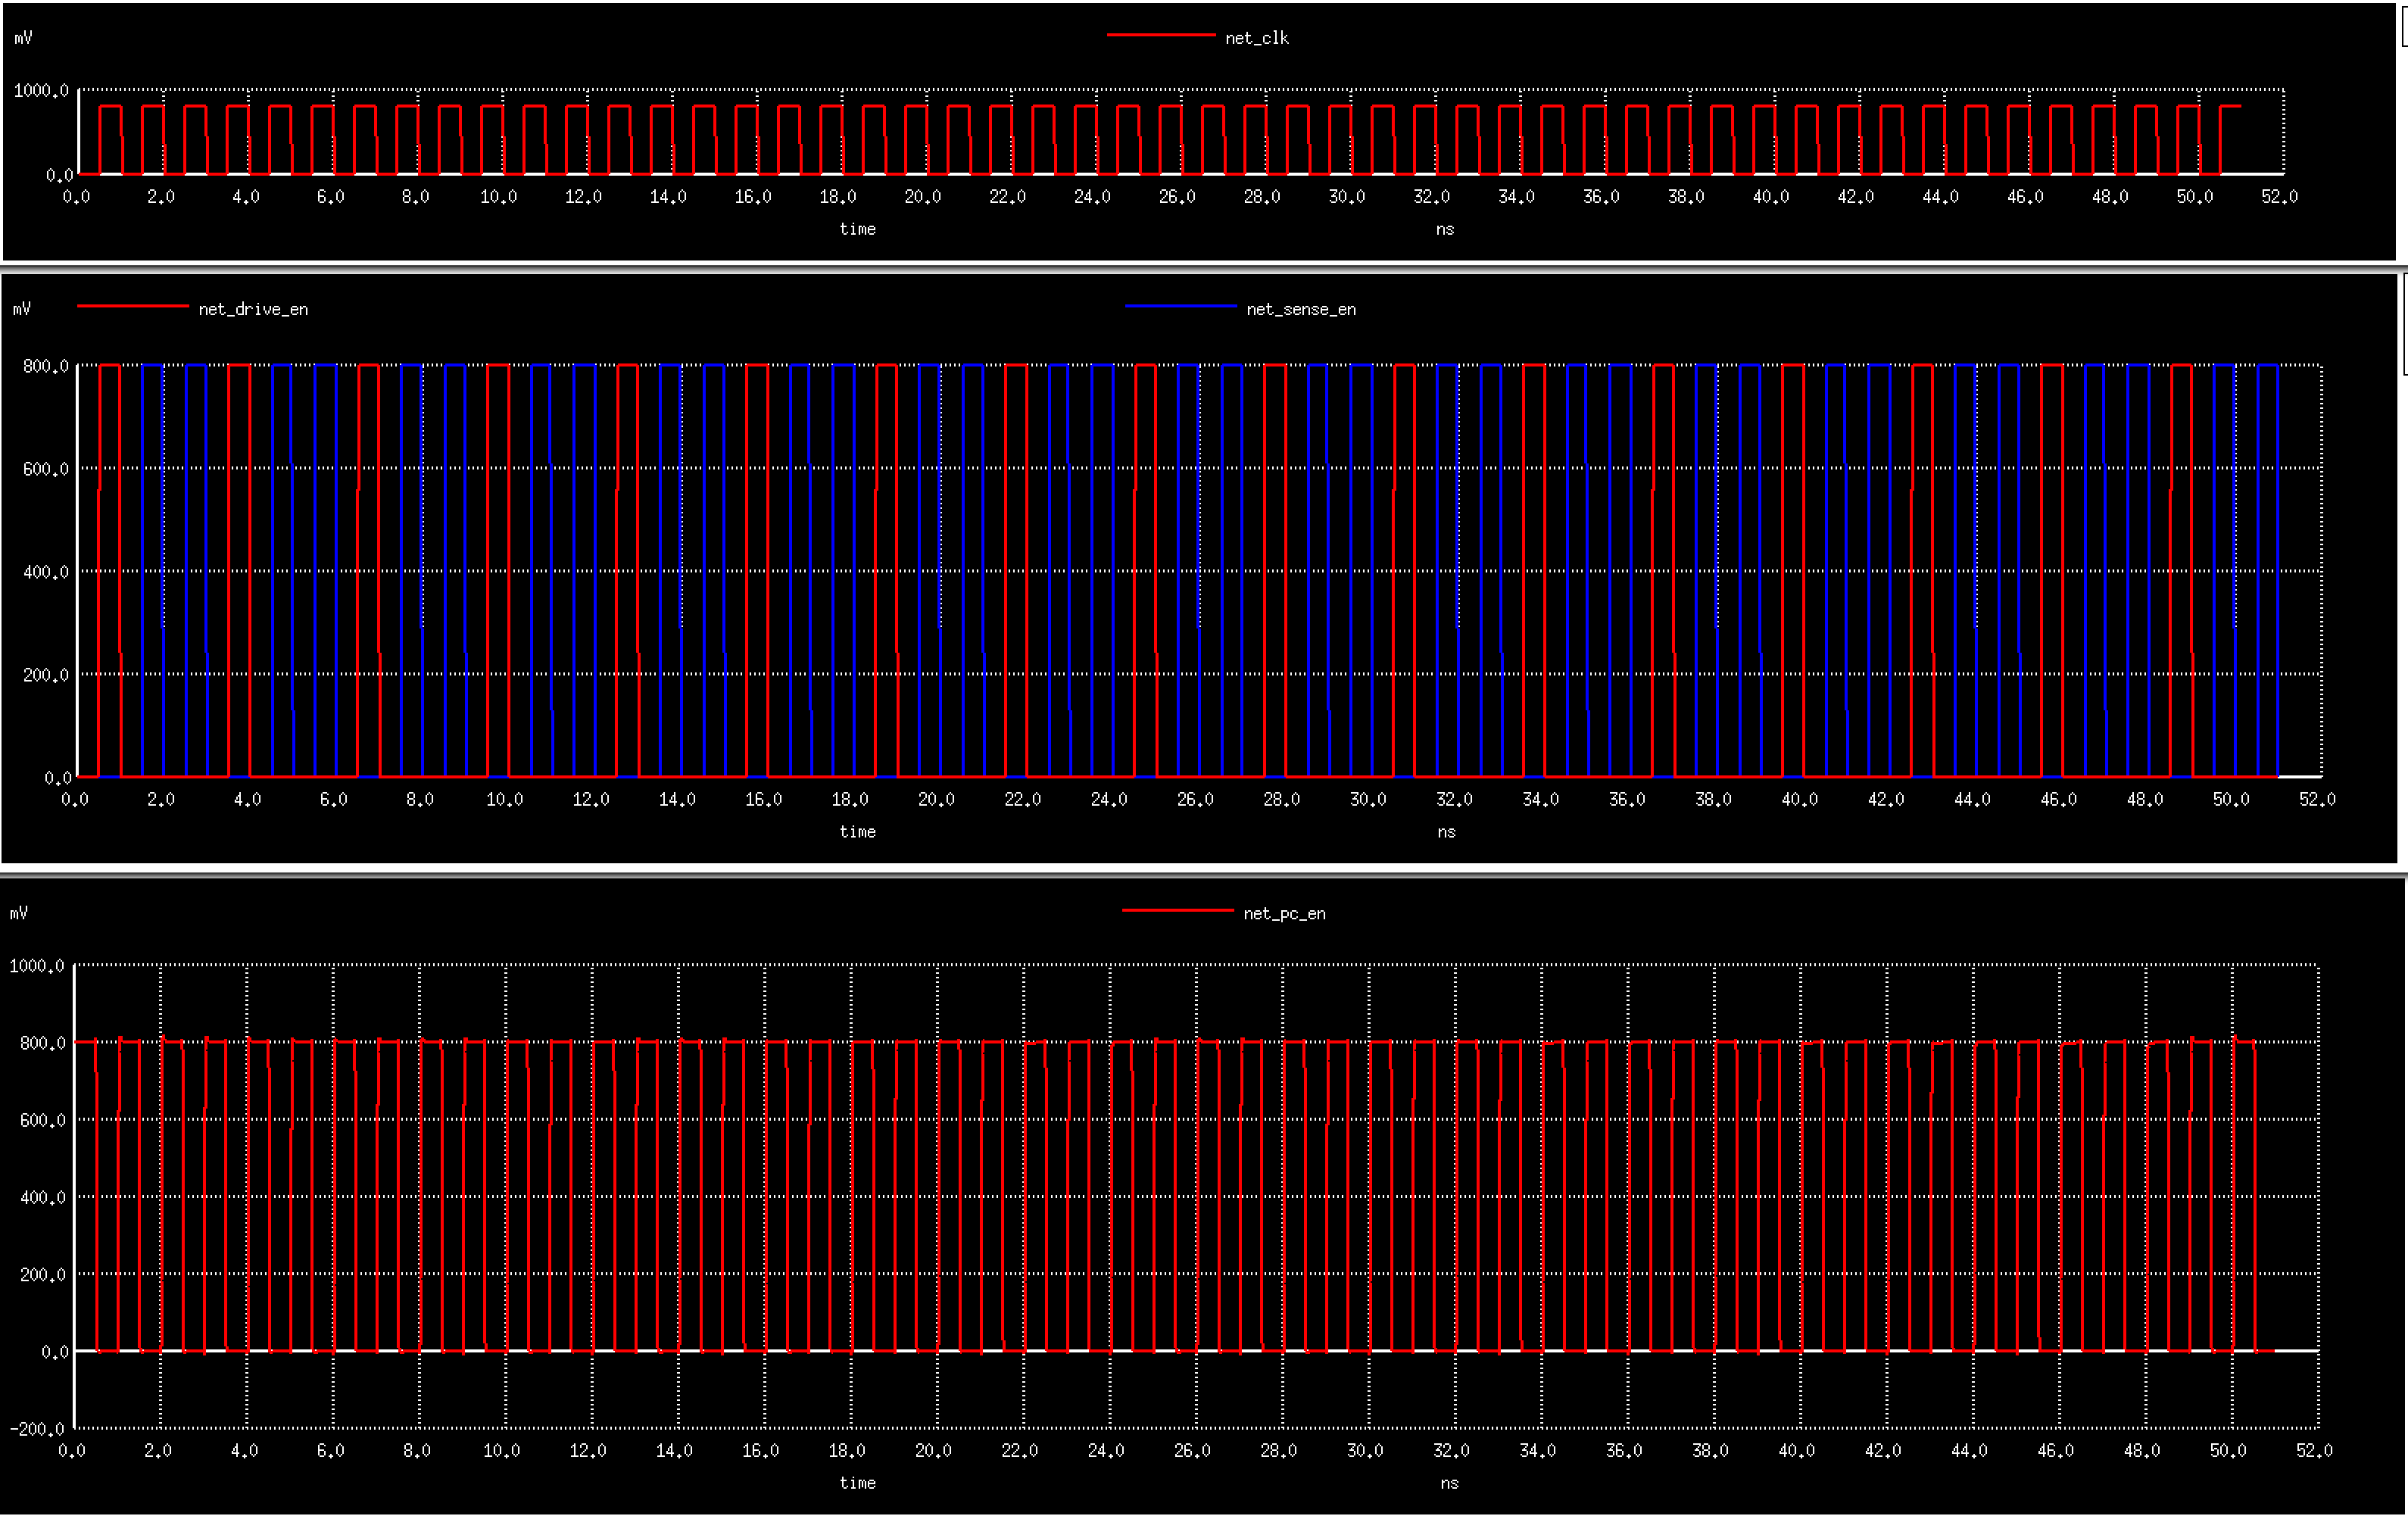
\includegraphics[scale=0.25]{memory16x16TestWaveformCtlInputs}
	\caption{16x16 RAM Test Control Inputs}
	\label{fig:memory16x16TestWaveformCtlInputs}
\end{figure}

\subsection{Periphery Circuitry}

\subsubsection{Decoder}
\label{sec:decoder_design}
The decoder is a 4 to 16 bit decoder and will be used for the periphery circuitry of the memory cell in the top level design. The schematic (Figure \ref{fig:decoderSchematic}) has two parts: pre-decoding (Figure \ref{fig:decoderSchematicPreDecoder}) and output/reset (Figure \ref{fig:decoderSchematicReset}). The reset is active low so that when the reset is high, all outputs are driven according to the inputs and when reset is low, all outputs are driven low. 

\begin{figure}[H]
	\centering
	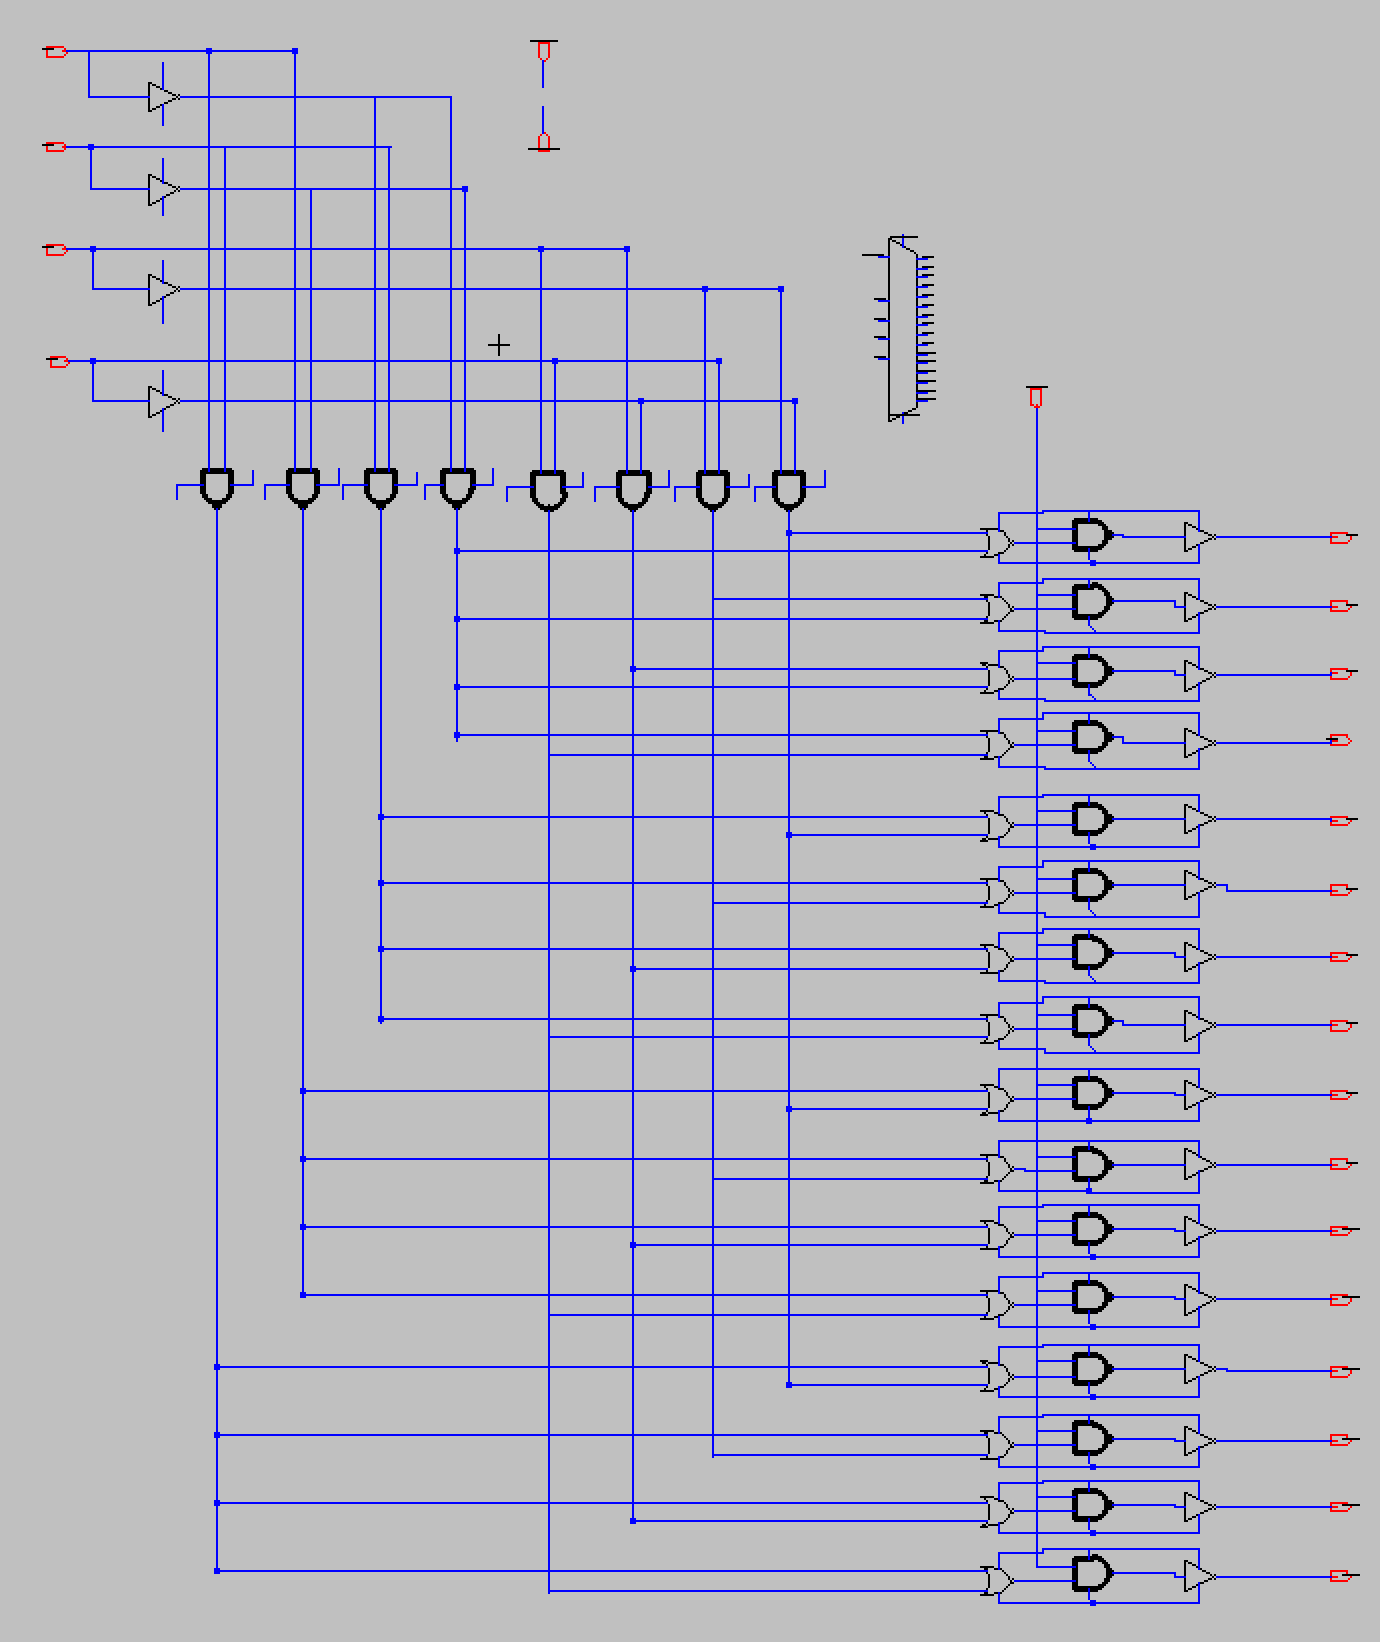
\includegraphics[scale=0.35]{decoderSchematic}
	\caption{4 to 16 Bit Decoder Schematic}
	\label{fig:decoderSchematic}
\end{figure}

\begin{figure}[H]
	\centering
	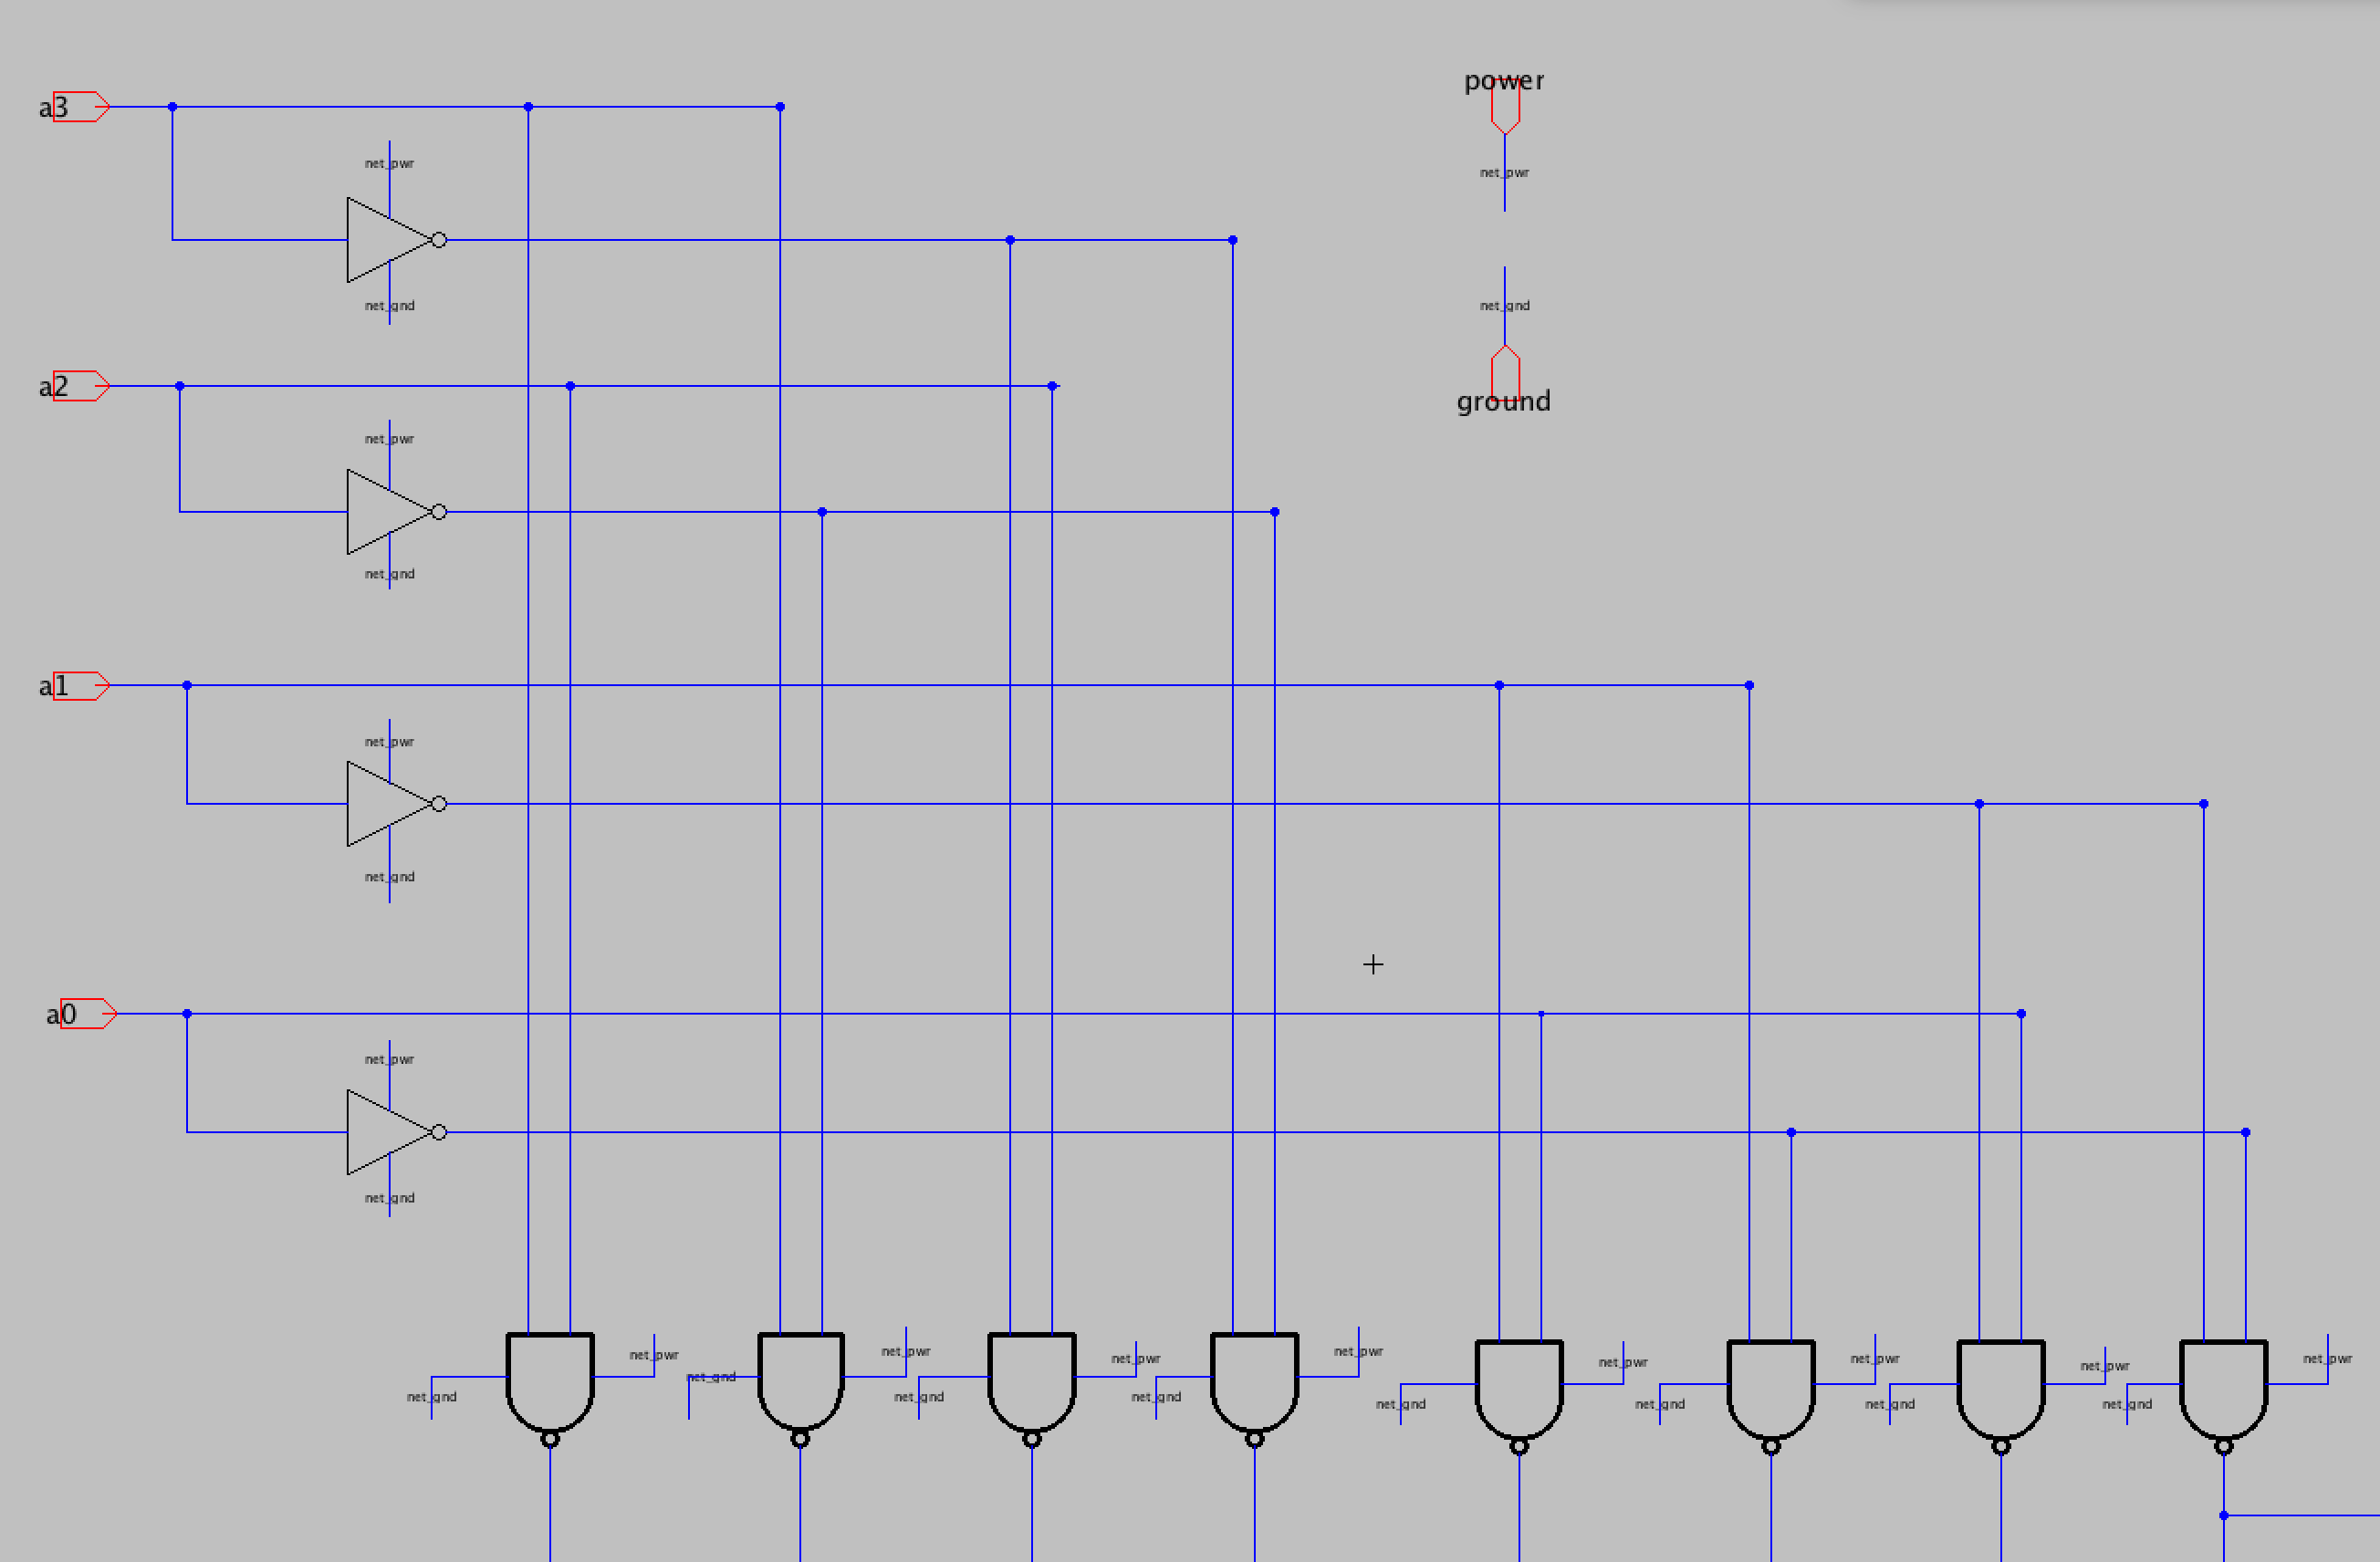
\includegraphics[scale=0.25]{decoderSchematicPreDecoder}
	\caption{4 to 16 Bit Pre-Decoder}
	\label{fig:decoderSchematicPreDecoder}
\end{figure}

\begin{figure}[H]
	\centering
	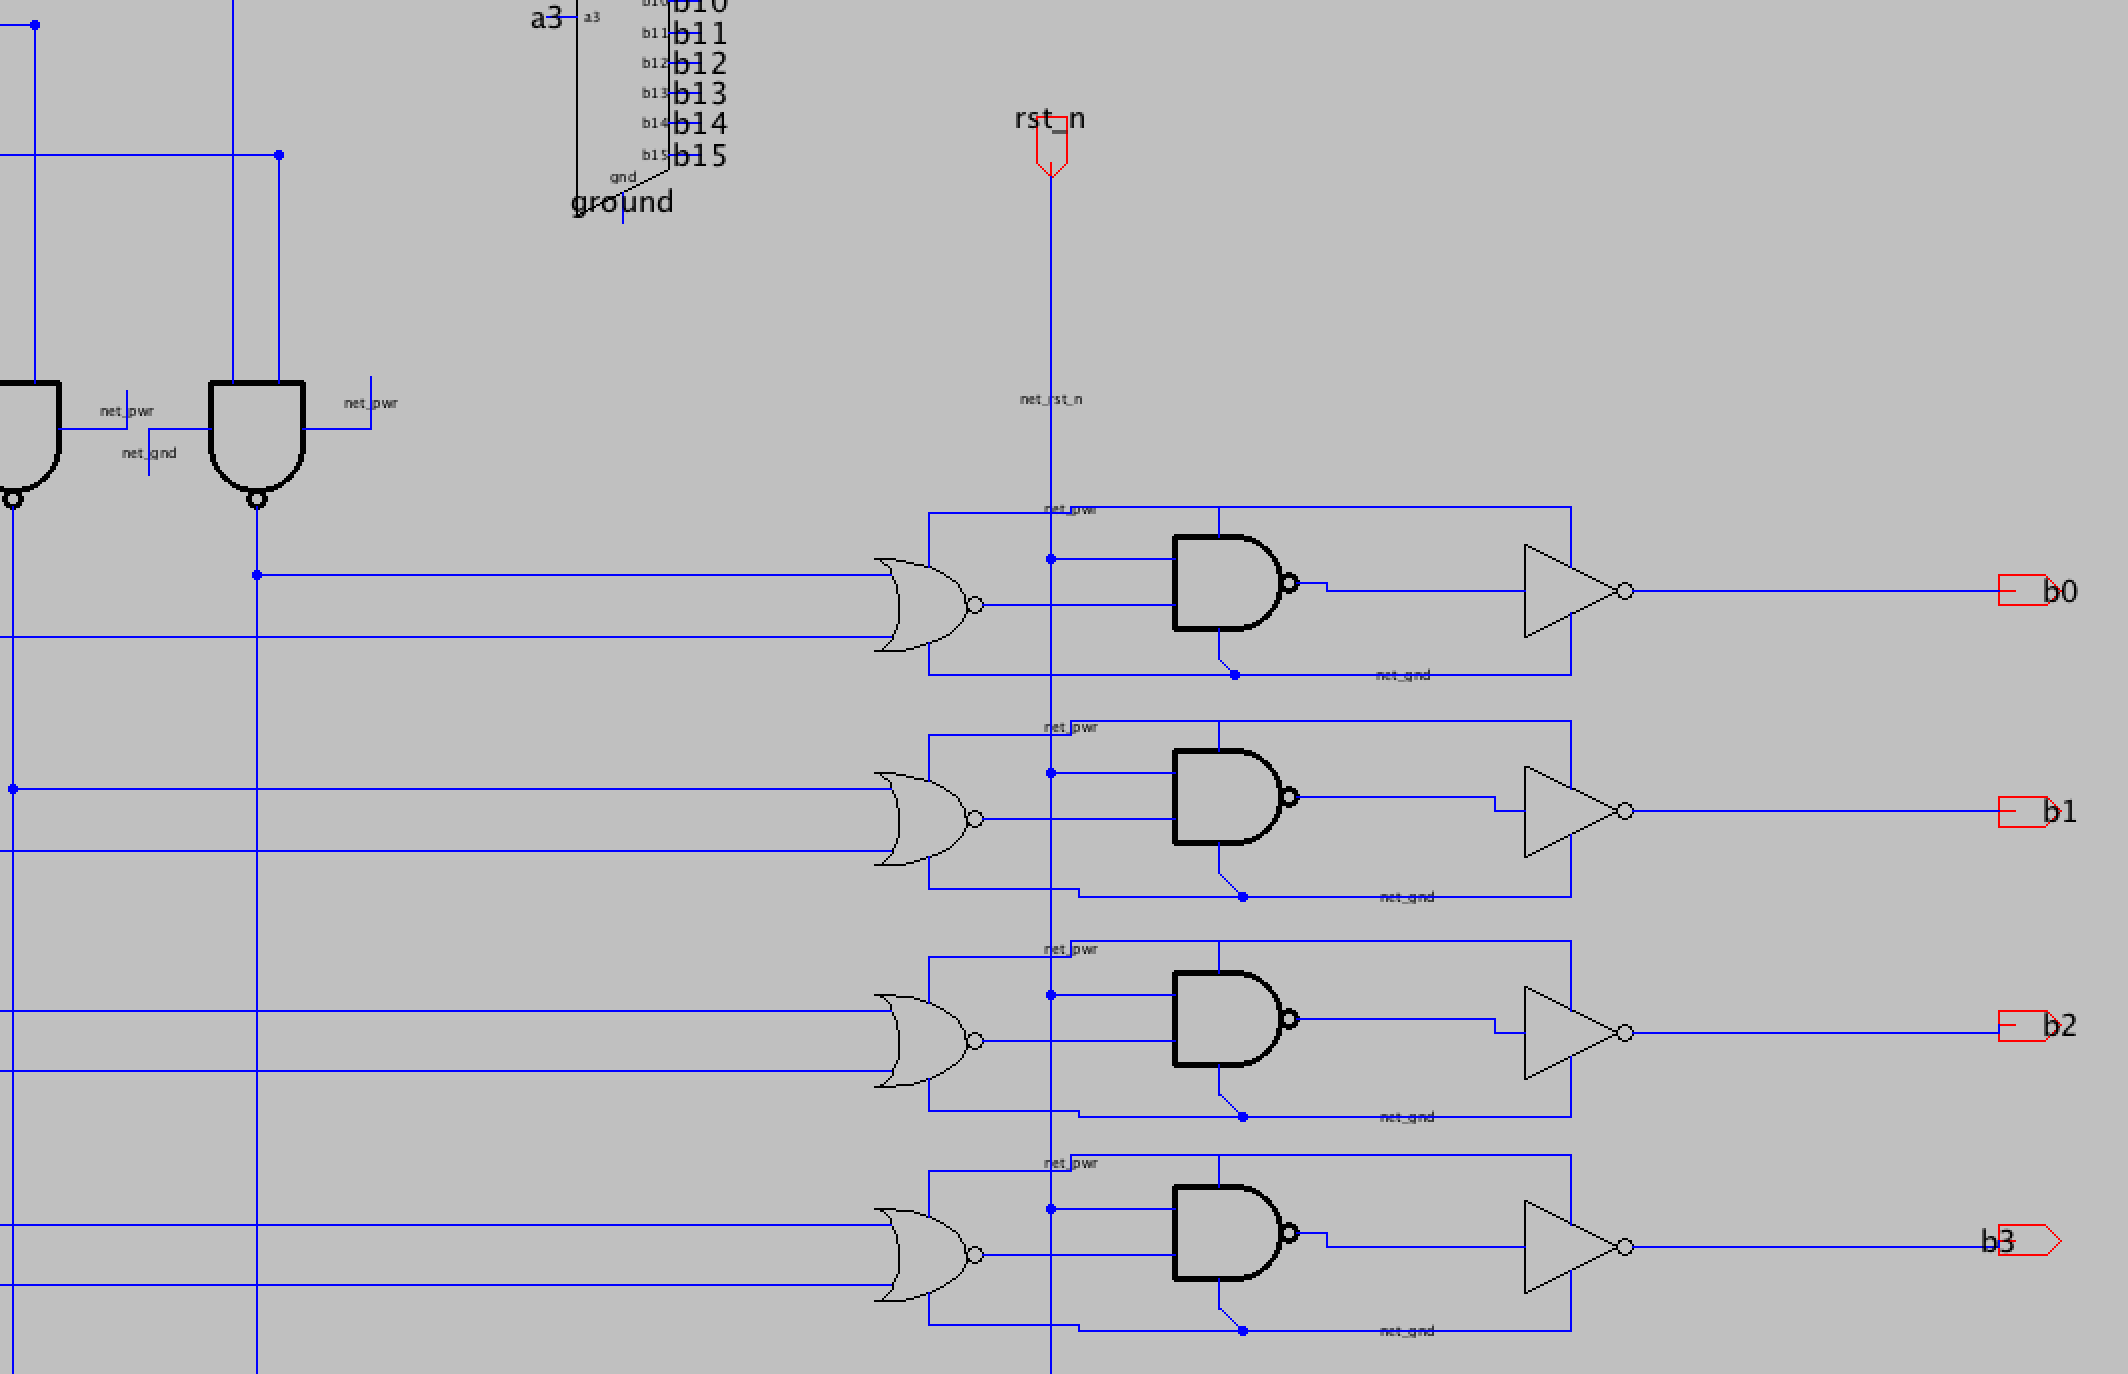
\includegraphics[scale=0.3]{decoderSchematicReset}
	\caption{4 to 16 Bit Decoder Output and Reset}
	\label{fig:decoderSchematicReset}
\end{figure}

\textbf{Correctness}\\
For correctness, we tested every possible input and verified outputs. The outputs from the test schematic (Figure \ref{fig:decoderTestWithResetSchematic}) are working as expected--shown in Figure \ref{fig:decoderTestWithResetWaveform}. 

\begin{figure}[H]
	\centering
	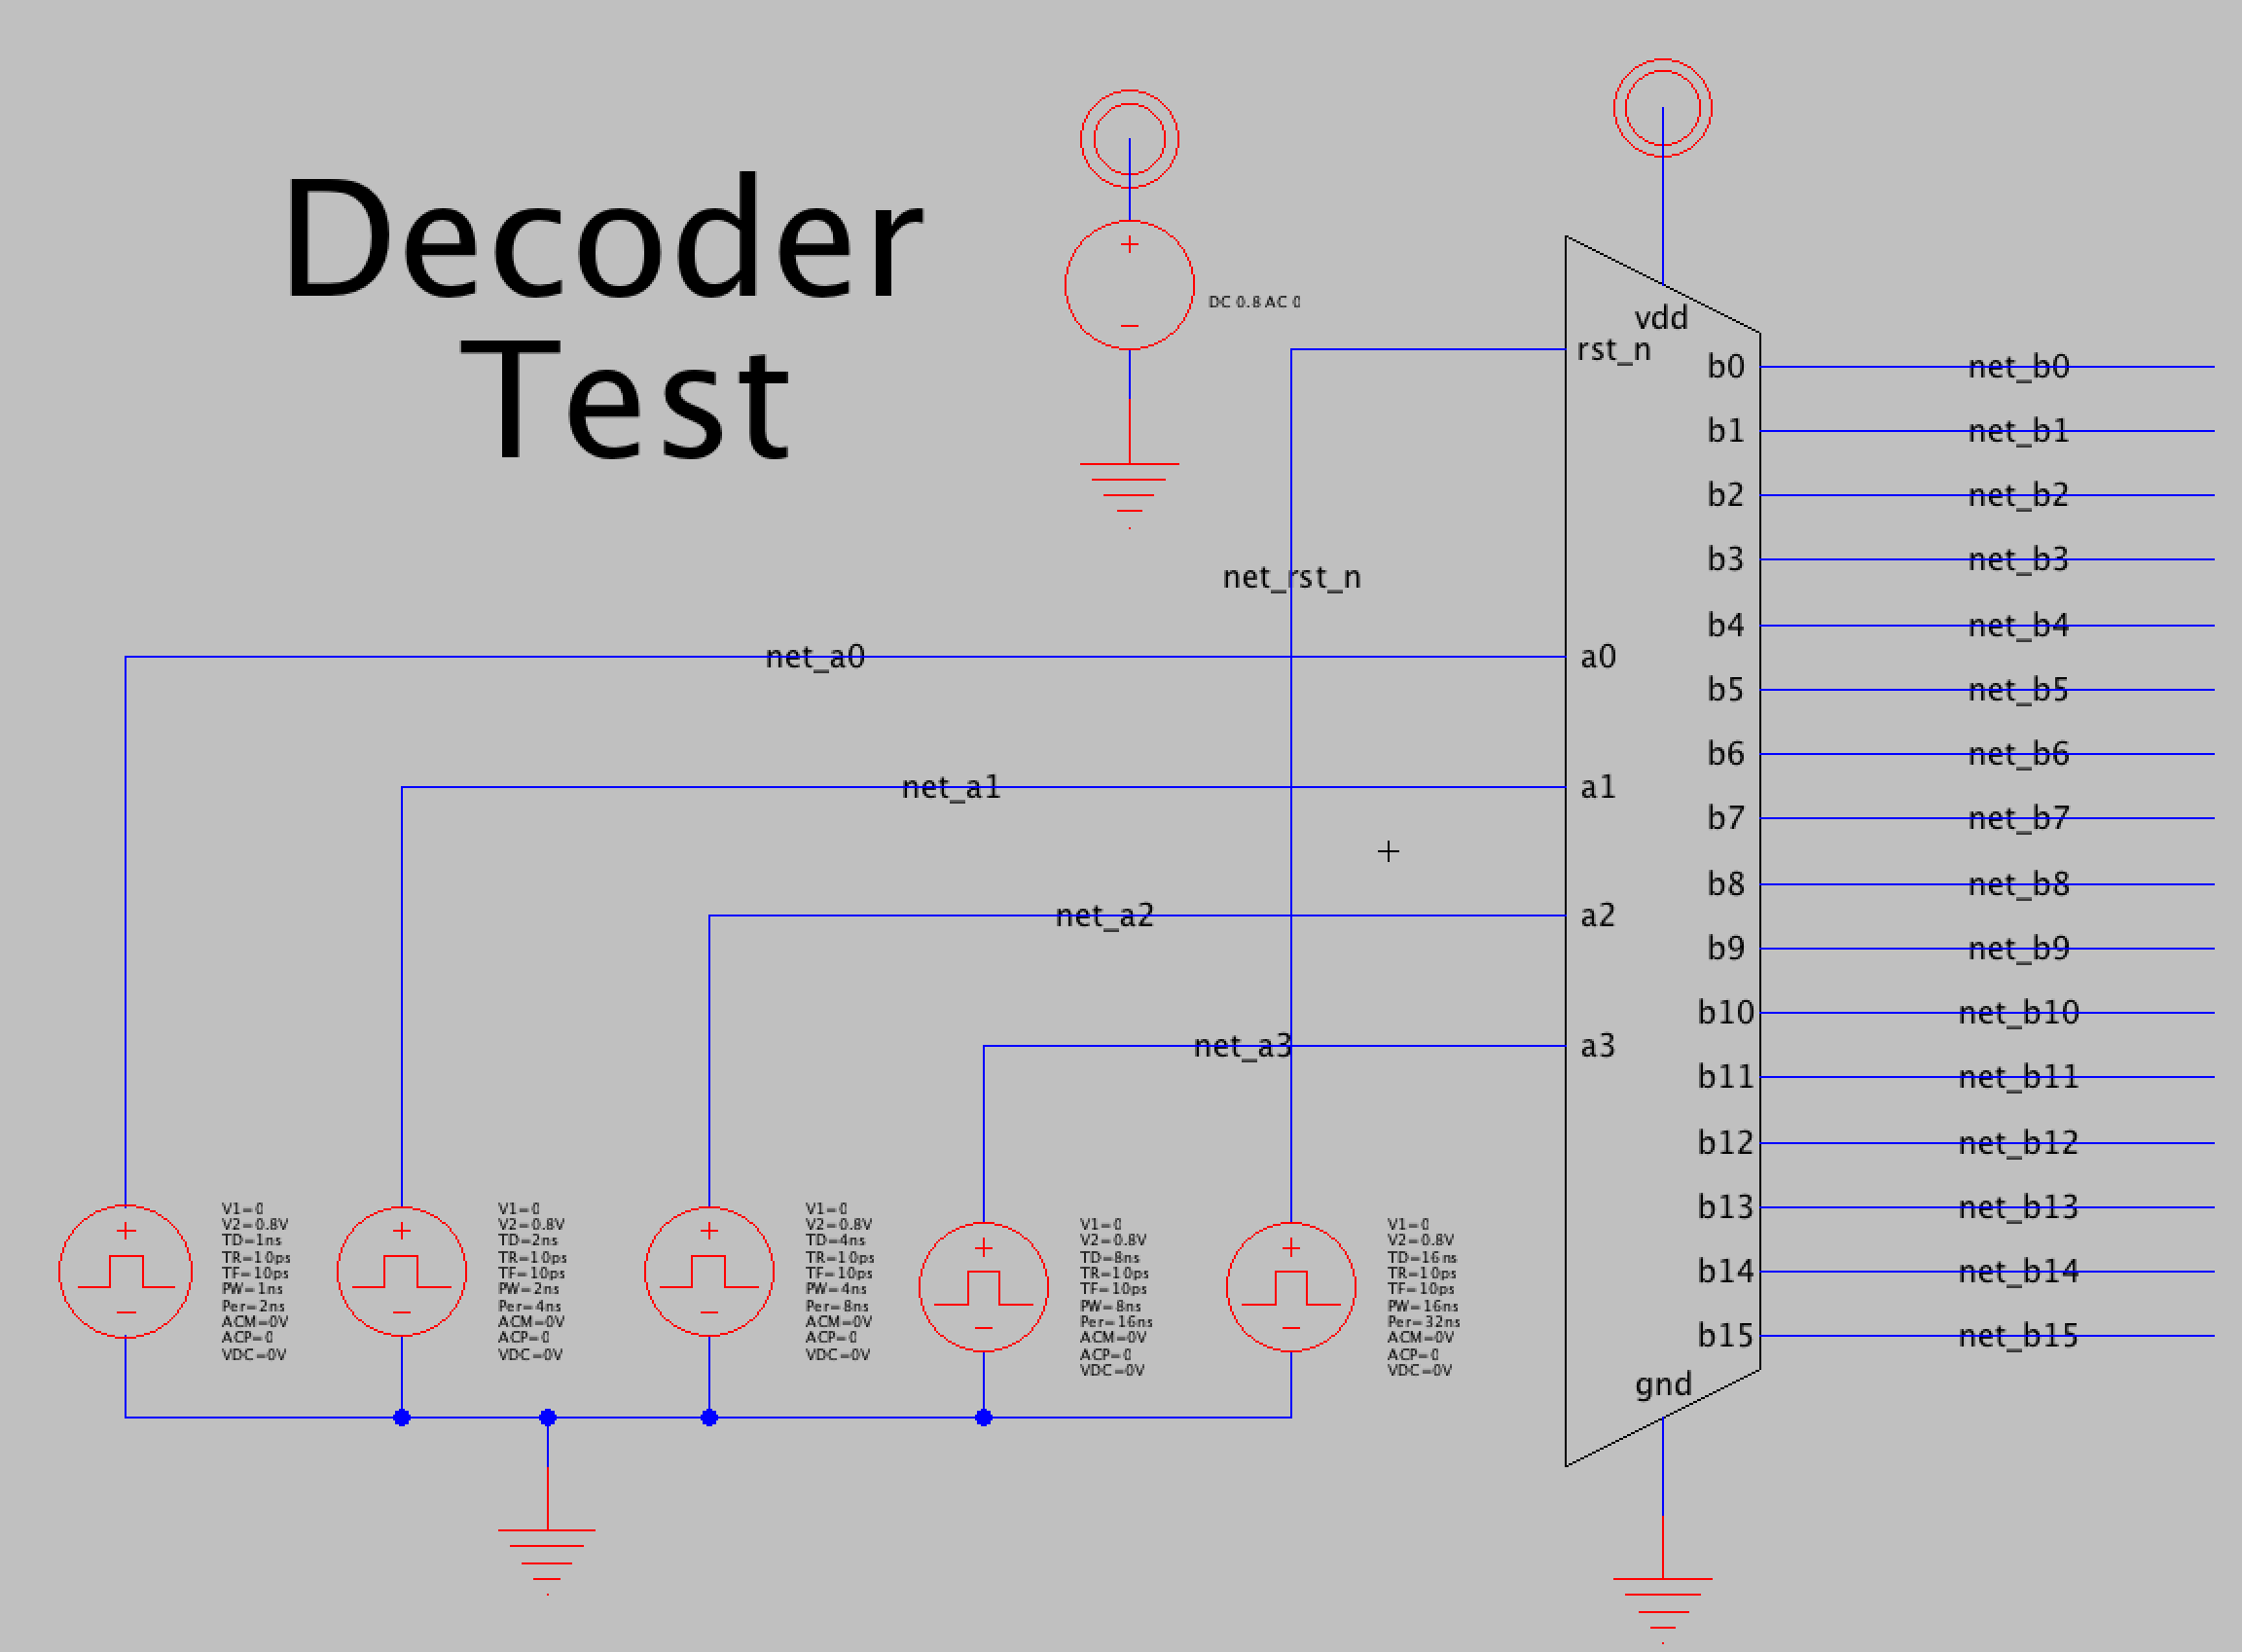
\includegraphics[scale=0.3]{decoderTestWithResetSchematic}
	\caption{4 to 16 Bit Decoder Test Schematic}
	\label{fig:decoderTestWithResetSchematic}
\end{figure}

\begin{figure}[H]
	\centering
	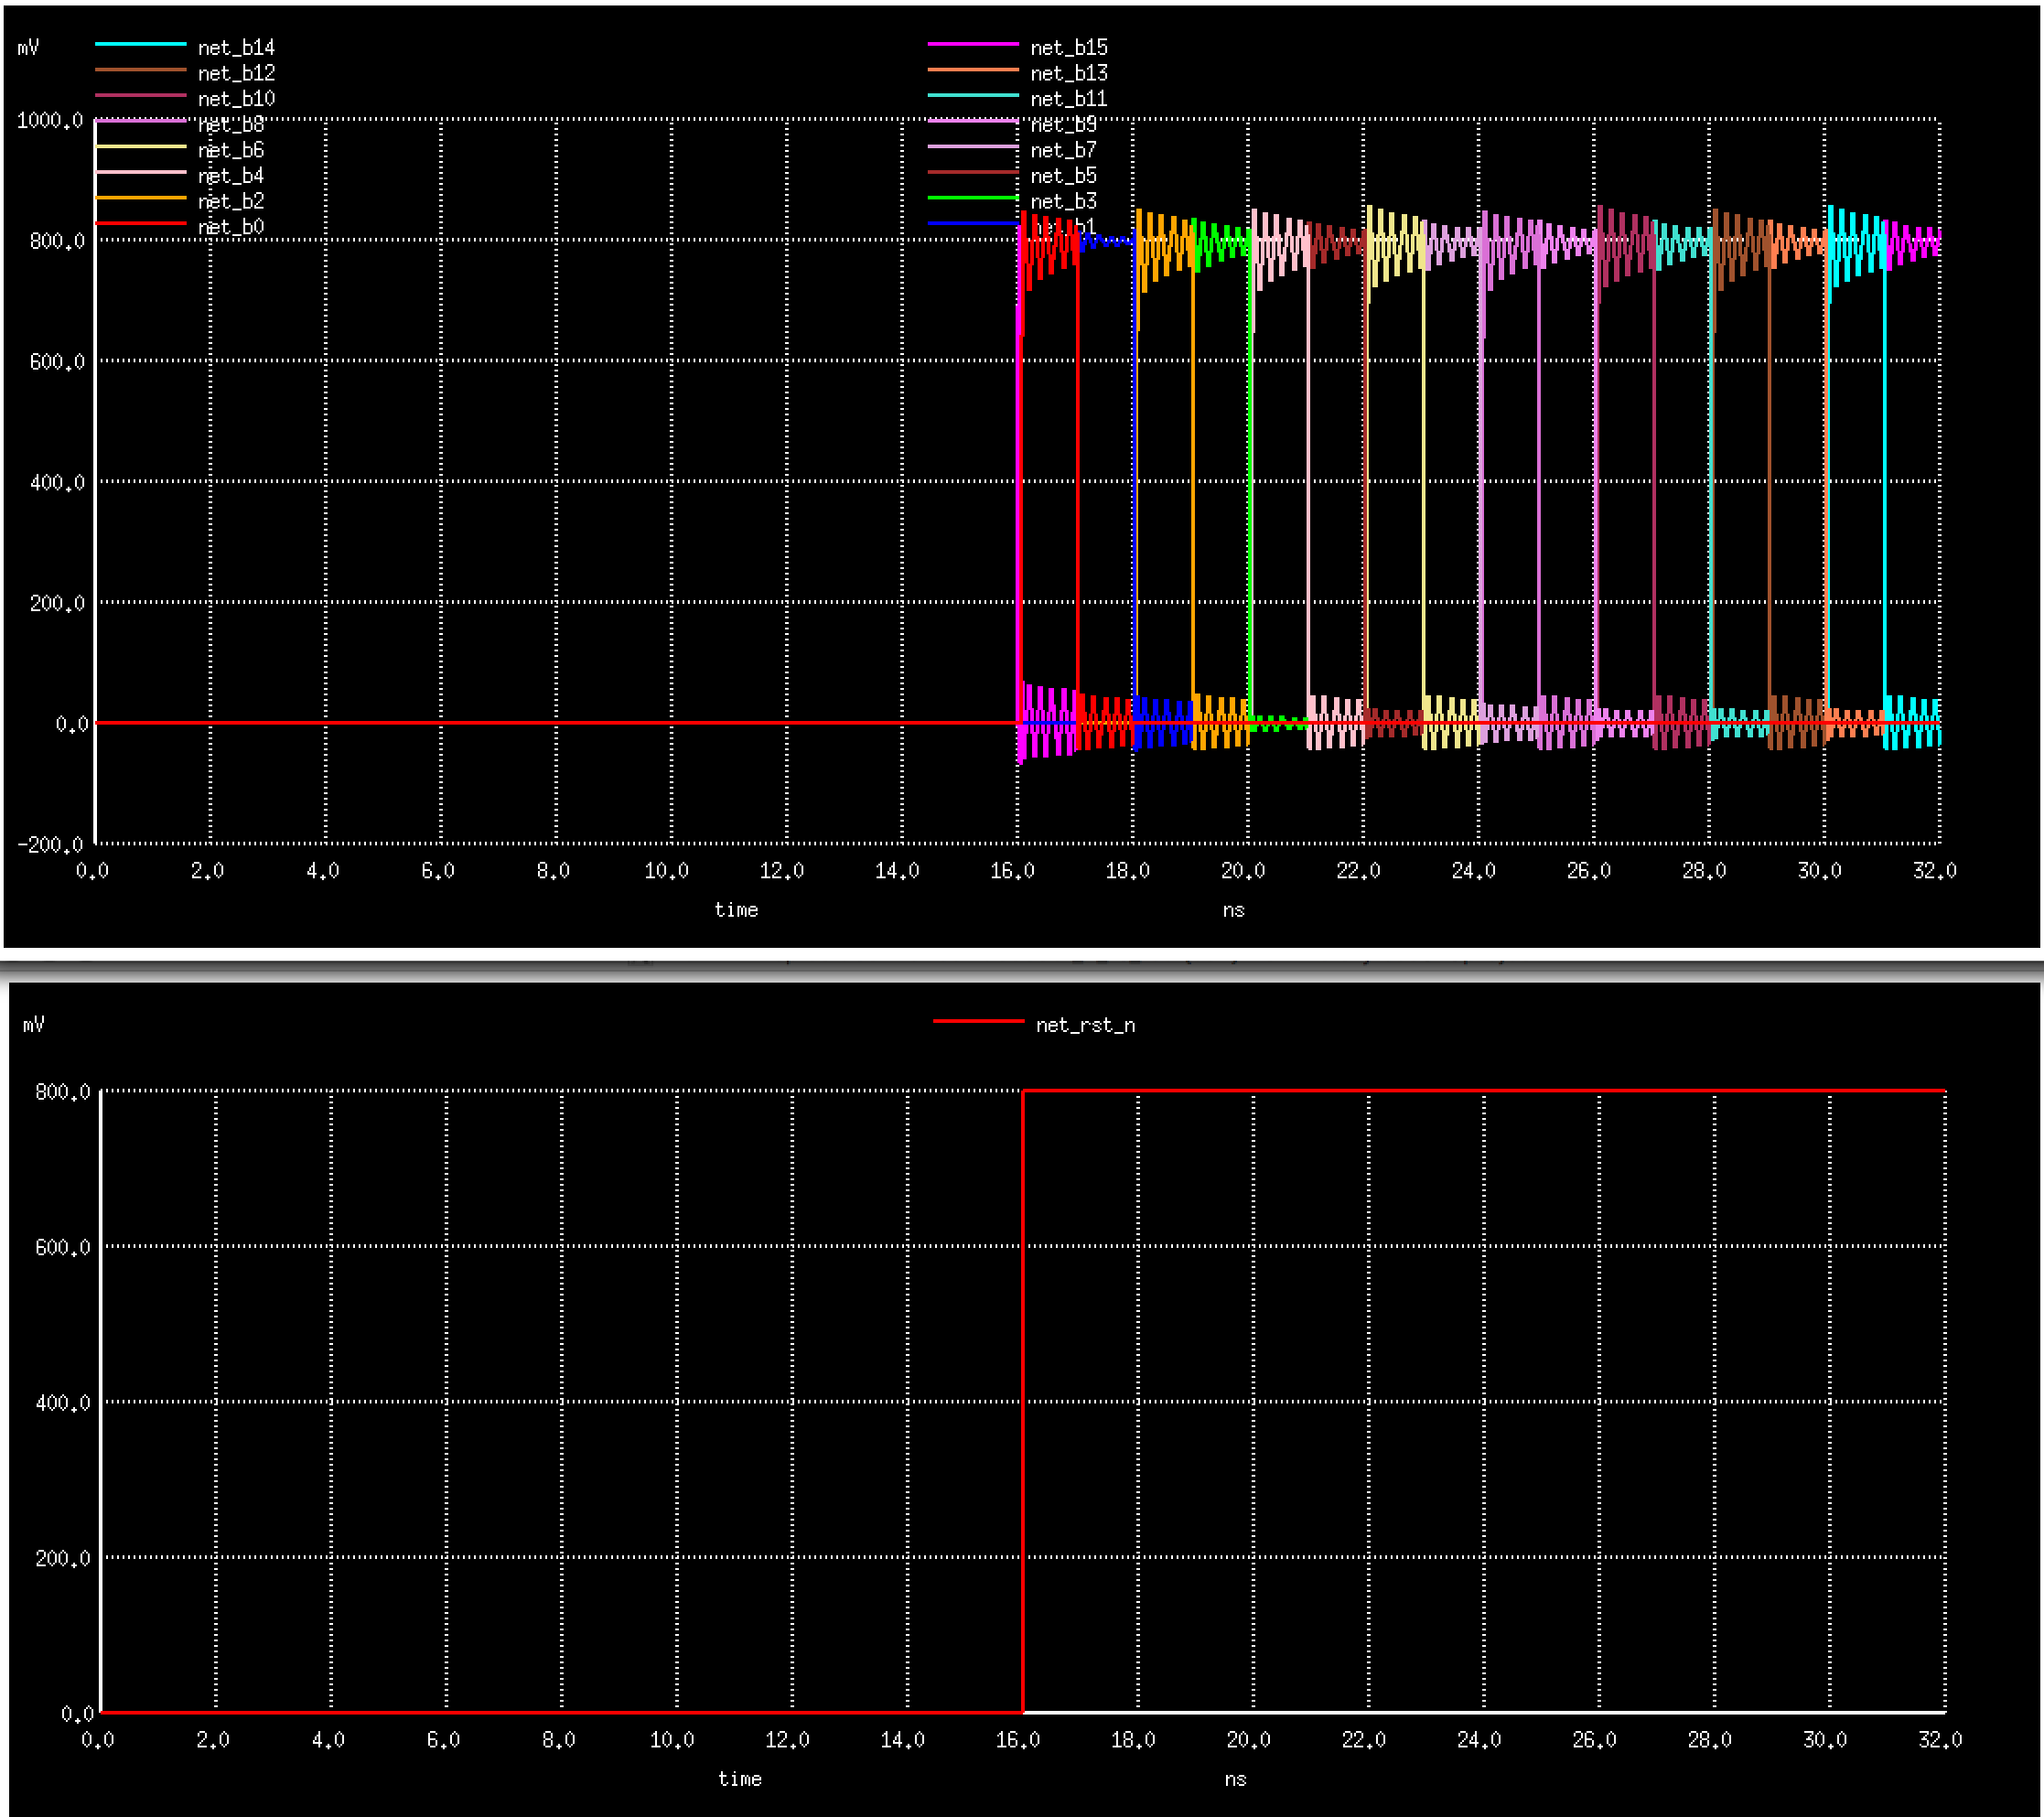
\includegraphics[scale=0.3]{decoderTestWithResetWaveform}
	\caption{4 to 16 Bit Decoder Test Waveform}
	\label{fig:decoderTestWithResetWaveform}
\end{figure}

\subsubsection{IO Register}
\label{sec:io_register_design}

\subsubsection{Clock Box}
\label{sec:clock_box_design}

\subsubsection{Control Logic}
\label{sec:control_logic_design}

\newpage
\subsection{Top Level}
The top level unites the 16x16 SRAM Memory (Section \ref{sec:16x16_sram_design}), Decoder (Section \ref{sec:decoder_design}), IO Registers (Section \ref{sec:io_register_design}), Clock Box (Section \ref{sec:clock_box_design}), and Control Logic (Section \ref{sec:control_logic_design}). 

\subsubsection{Schematic}
The entire schematic is below in Figure \ref{fig:topLevelSchematic}.

\begin{figure}[H]
	\centering
	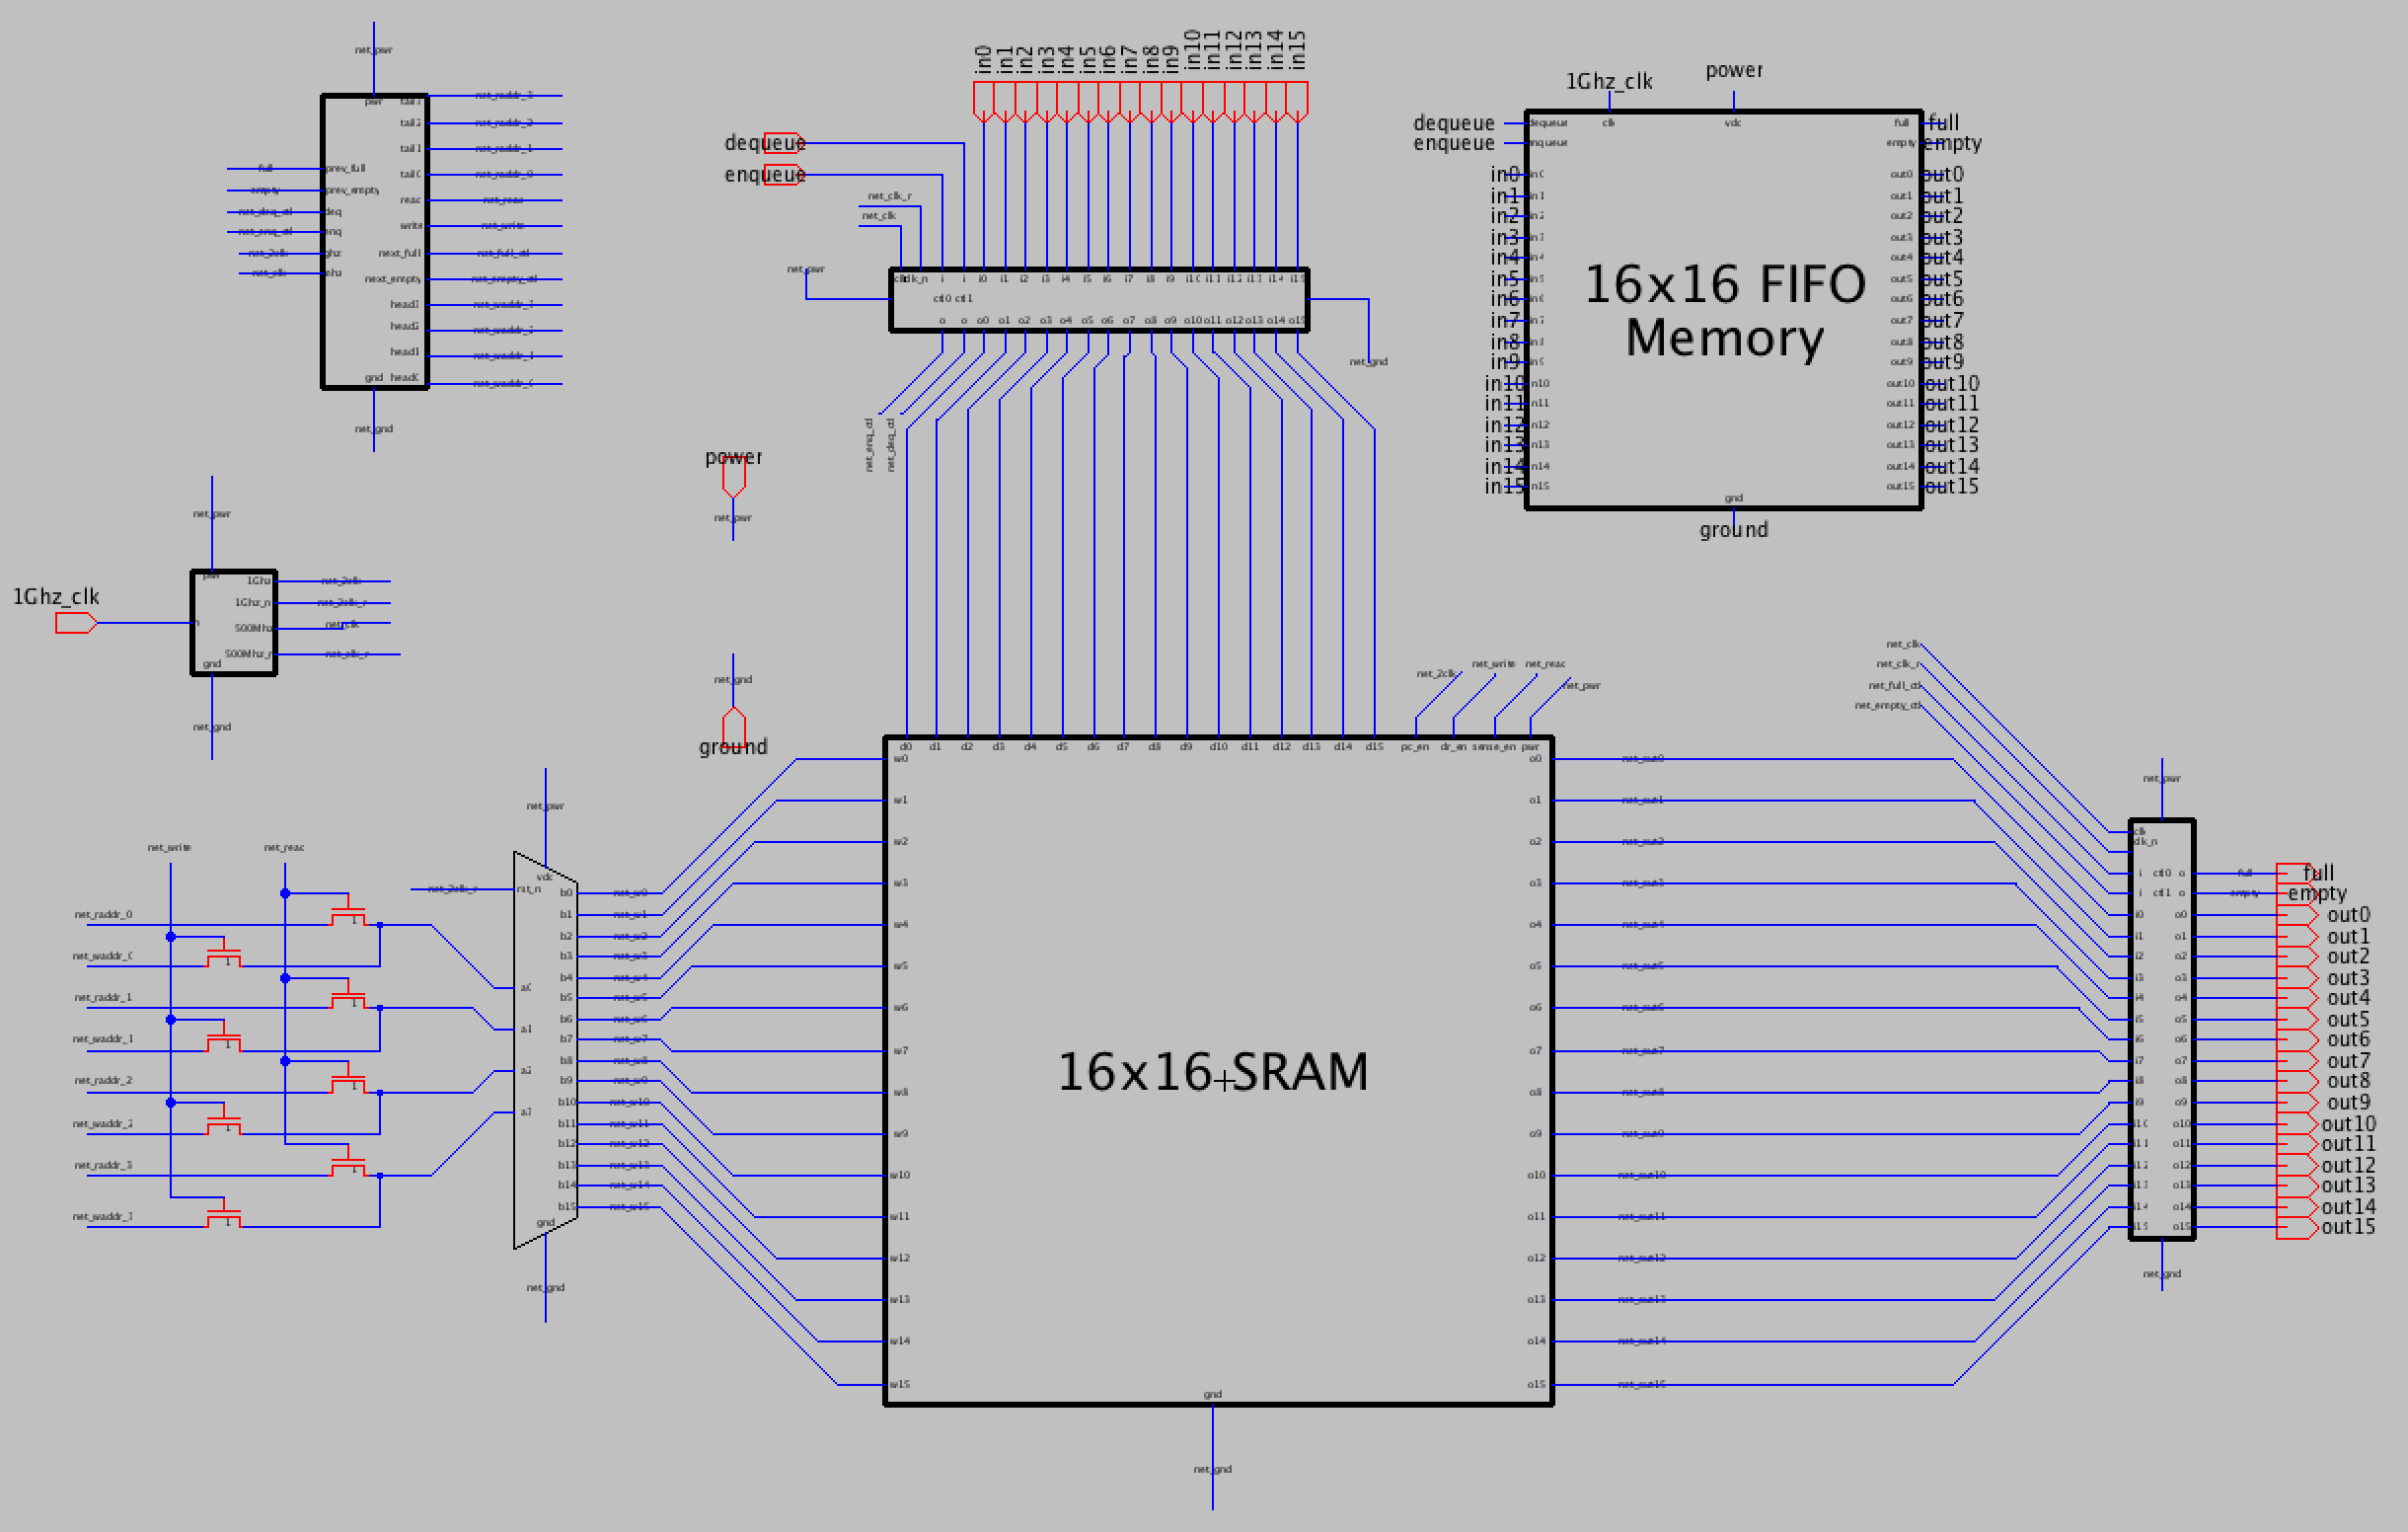
\includegraphics[scale=0.3]{topLevelSchematic}
	\caption{Top Level 16x16 FIFO Schematic}
	\label{fig:topLevelSchematic}
\end{figure}

The addresses are different for read and write, so we need an enable for both addresses. We use pass transistors to achieve this. The inputs of the decoder are robust enough to handle the $V_th$ drop caused by the enable transistor.

\begin{figure}[H]
	\centering
	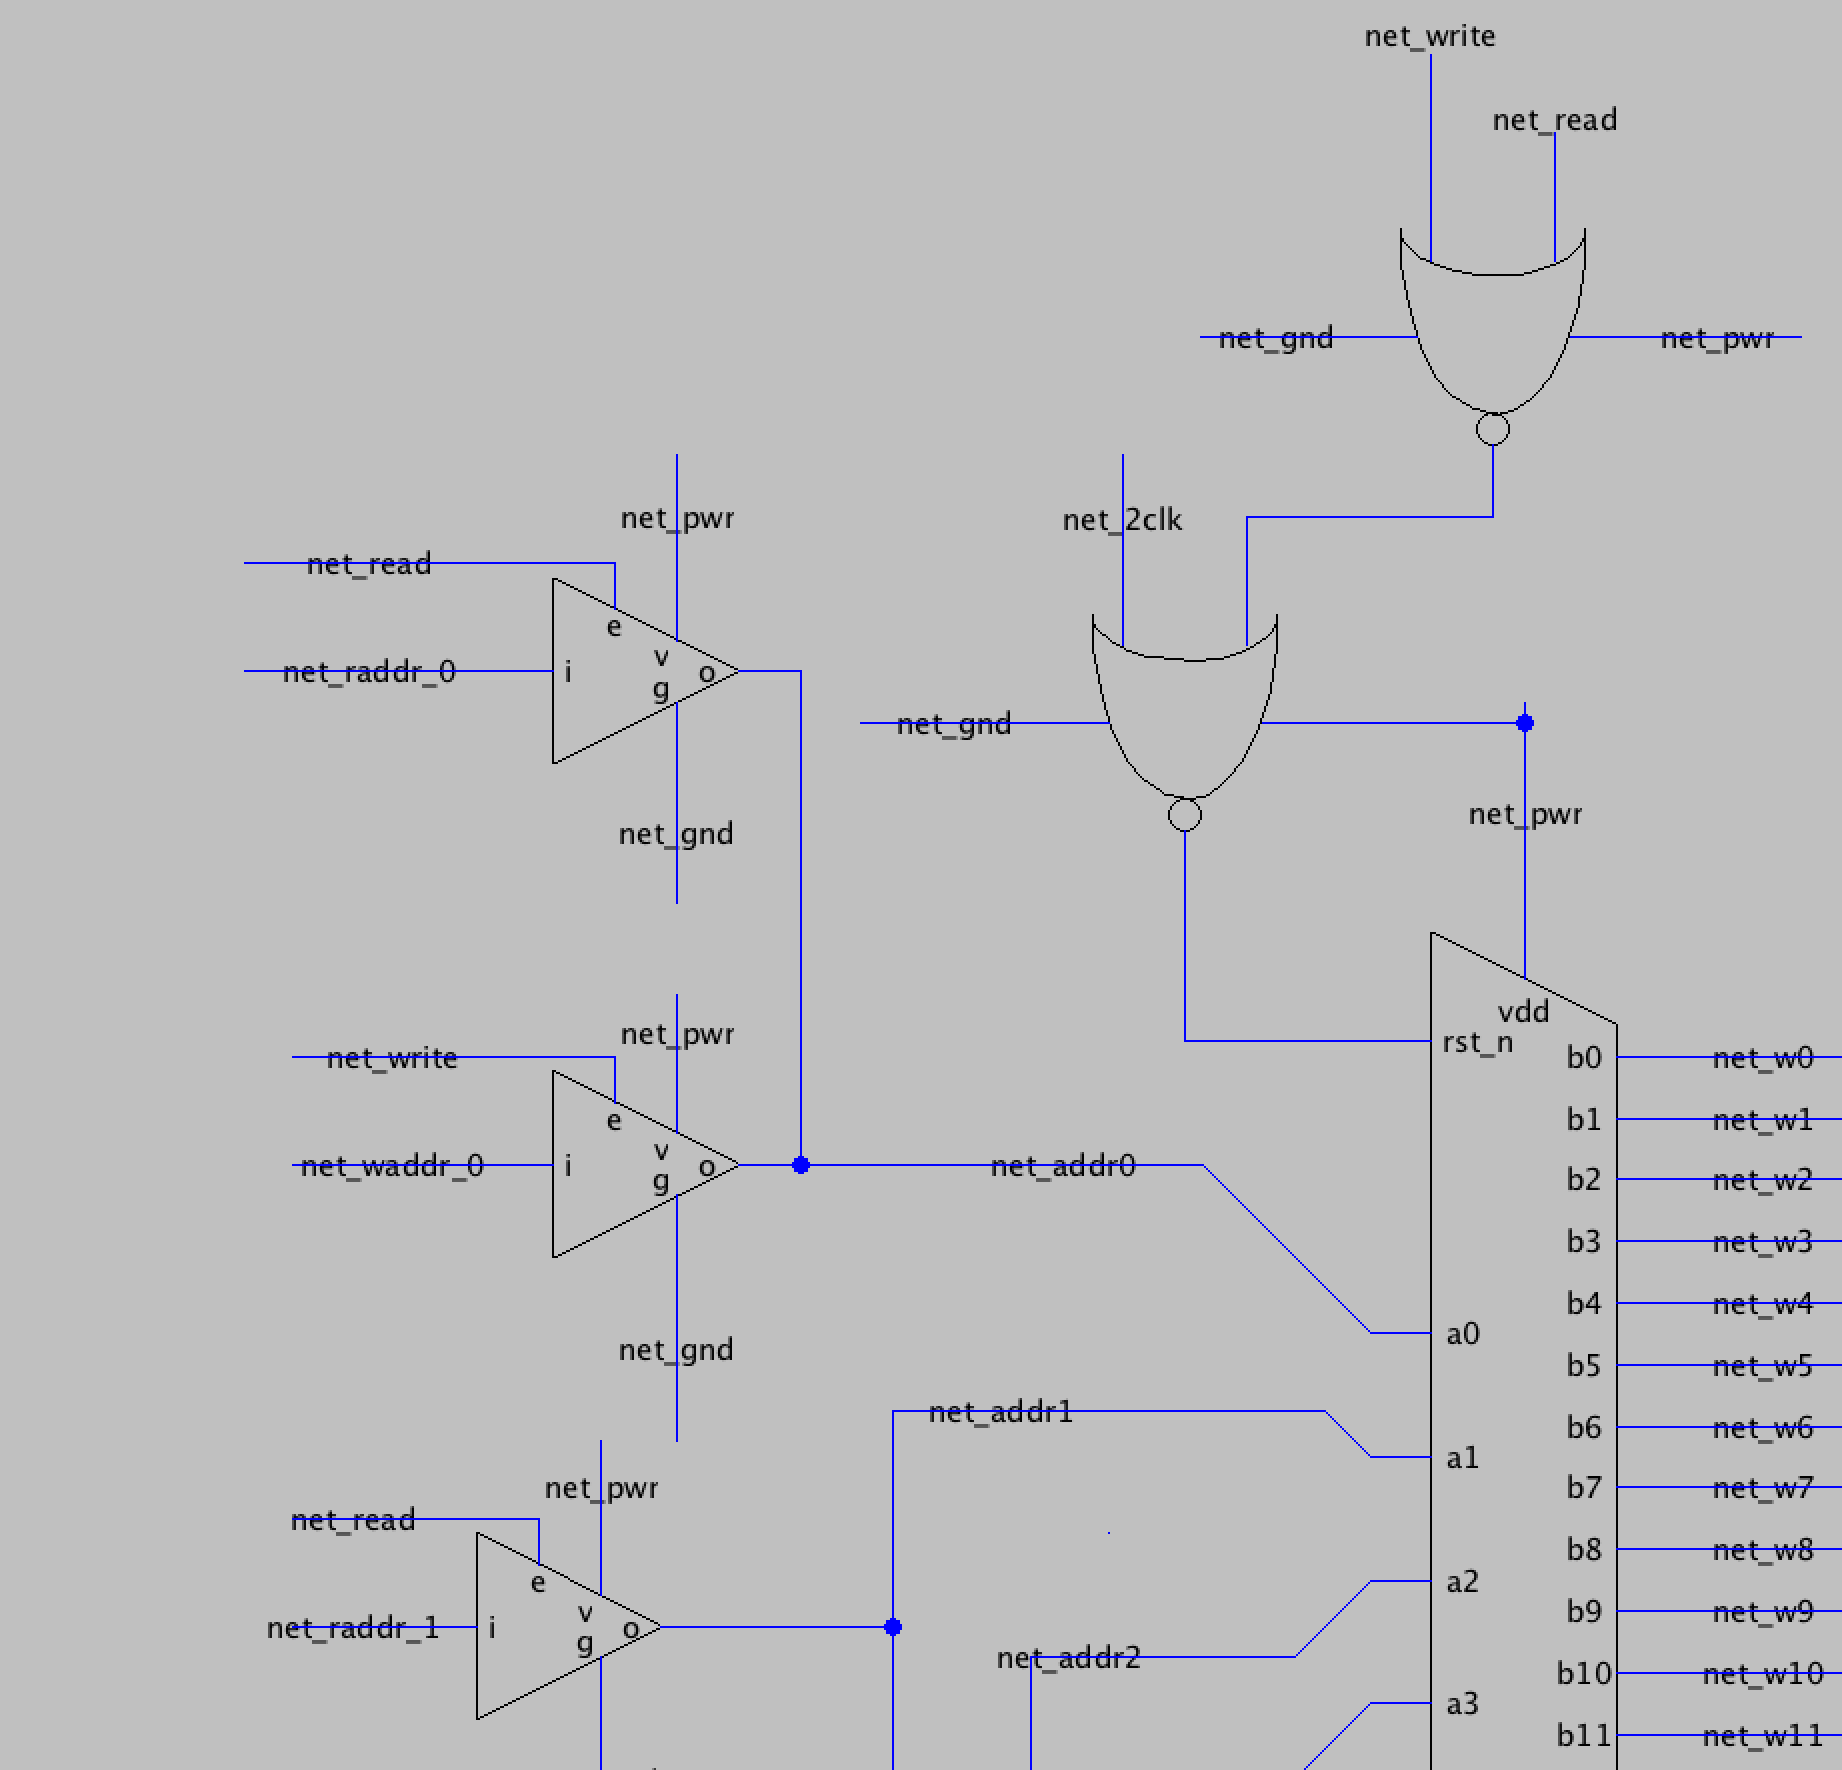
\includegraphics[scale=0.3]{topLevelSchematicLeft}
	\caption{Top Level 16x16 FIFO Schematic Address Input}
	\label{fig:topLevelSchematicLeft}
\end{figure}

The clock box generates the clock for the design $net\_clk$, which runs at the requested 500MHz. We need to use the multiplied clock ($net\_2clk$) for performing two operations in a single 500MHz clock cycle. 

\begin{figure}[H]
	\centering
	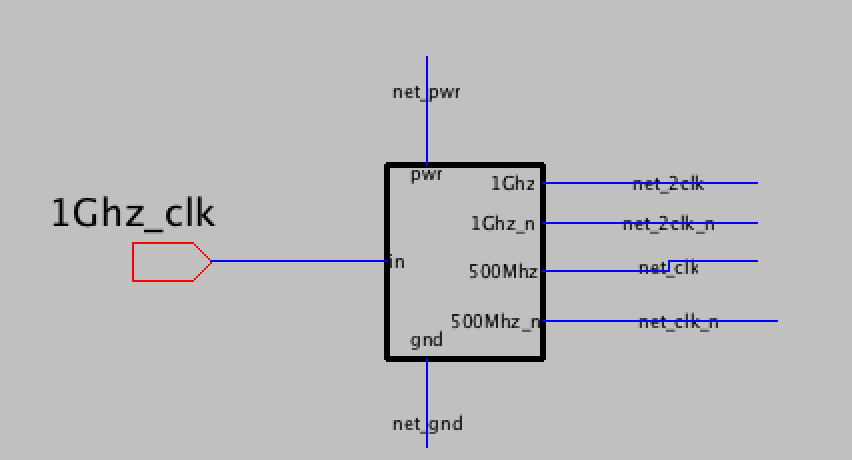
\includegraphics[scale=0.65]{topLevelSchematicClockBox}
	\caption{Top Level 16x16 FIFO Schematic Clock Module}
	\label{fig:topLevelSchematicClockBox}
\end{figure}

The logic module generates the read and write addresses, full and empty signals, and read and write signals.

\begin{figure}[H]
	\centering
	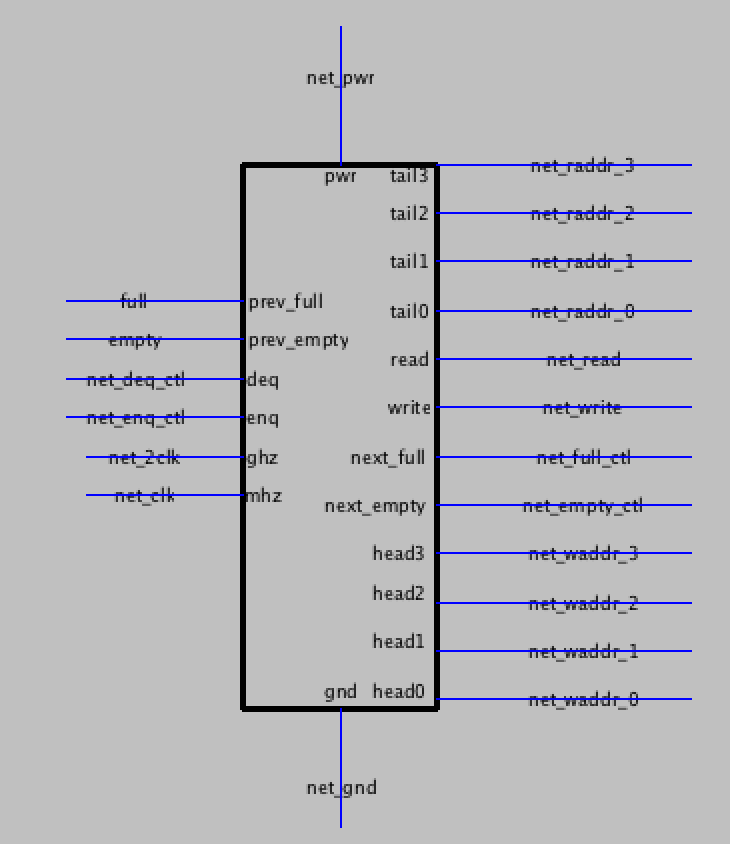
\includegraphics[scale=0.65]{topLevelSchematicLogic}
	\caption{Top Level 16x16 FIFO Schematic Logic Module}
	\label{fig:topLevelSchematicLogic}
\end{figure}

The input uses the IO Register to hold all input and output values and guarantee steady inputs.

\begin{figure}[H]
	\centering
	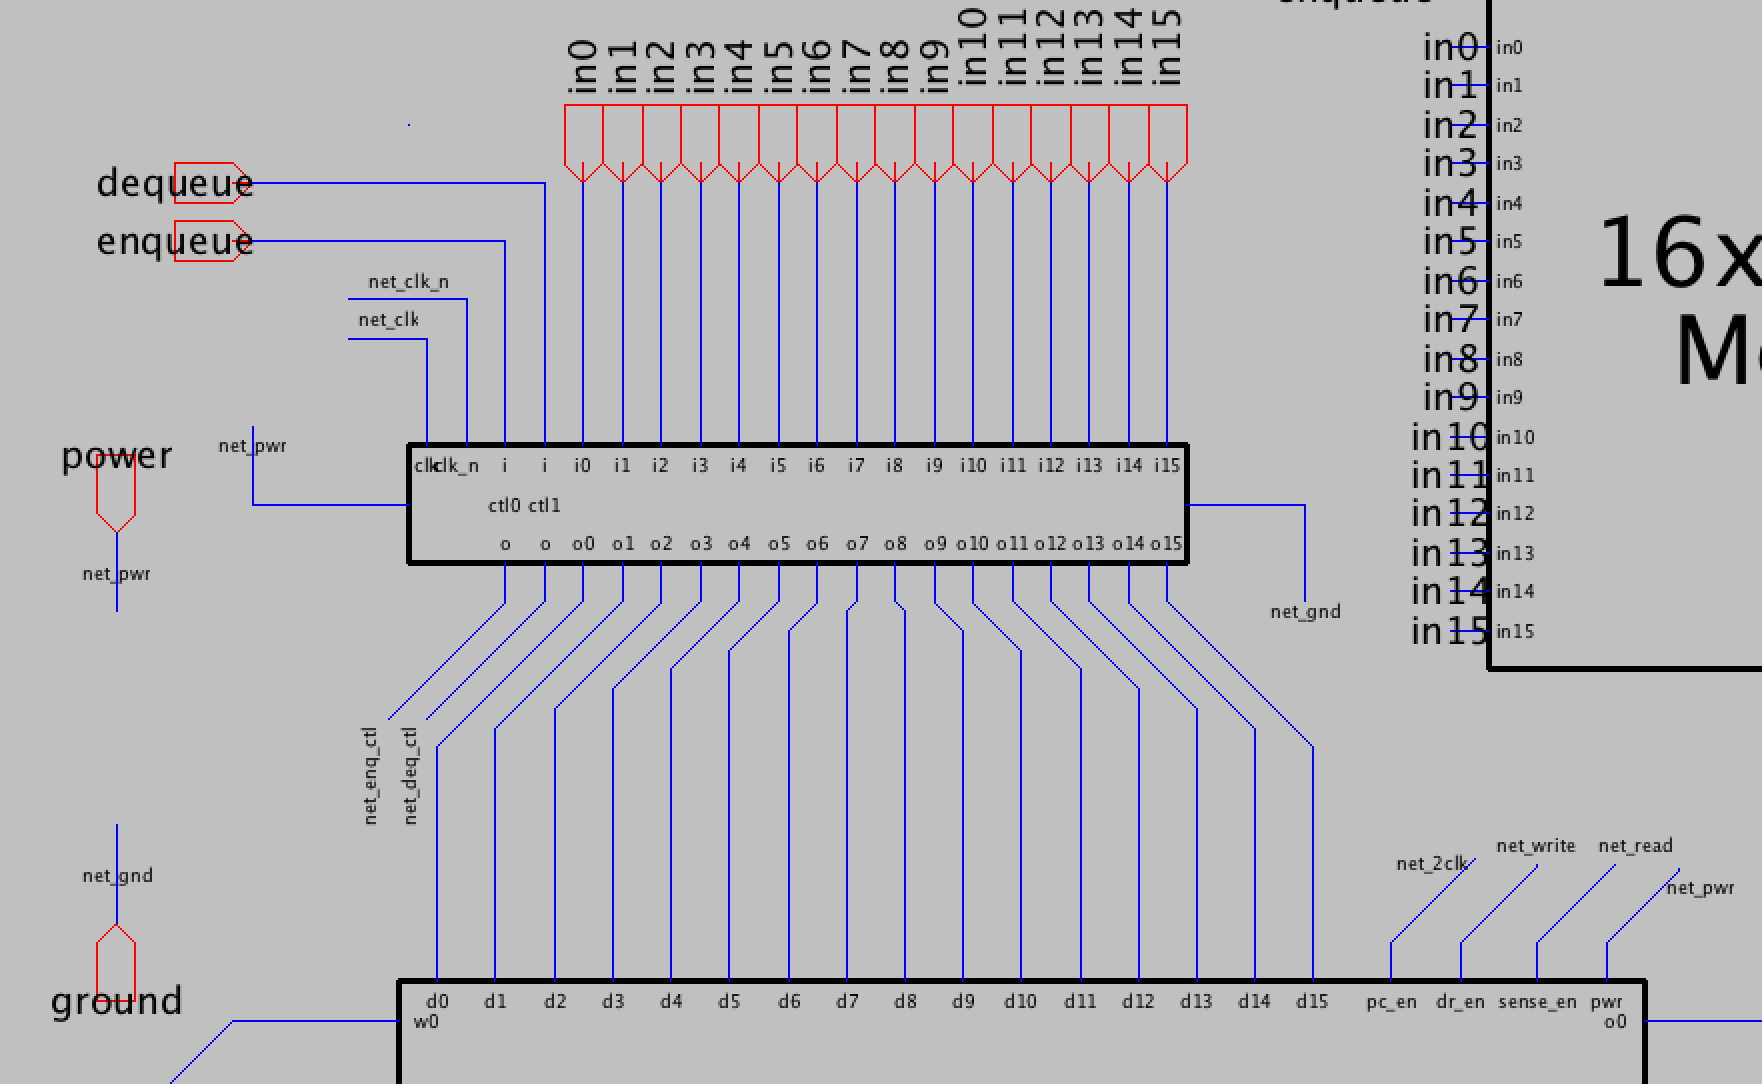
\includegraphics[scale=0.4]{topLevelSchematicTop}
	\caption{Top Level 16x16 FIFO Schematic Data Input}
	\label{fig:topLevelSchematicTop}
\end{figure}

The output register is latched on the edge of the 16x16 RAM's output signal and holds the values returning to the user.

\begin{figure}[H]
	\centering
	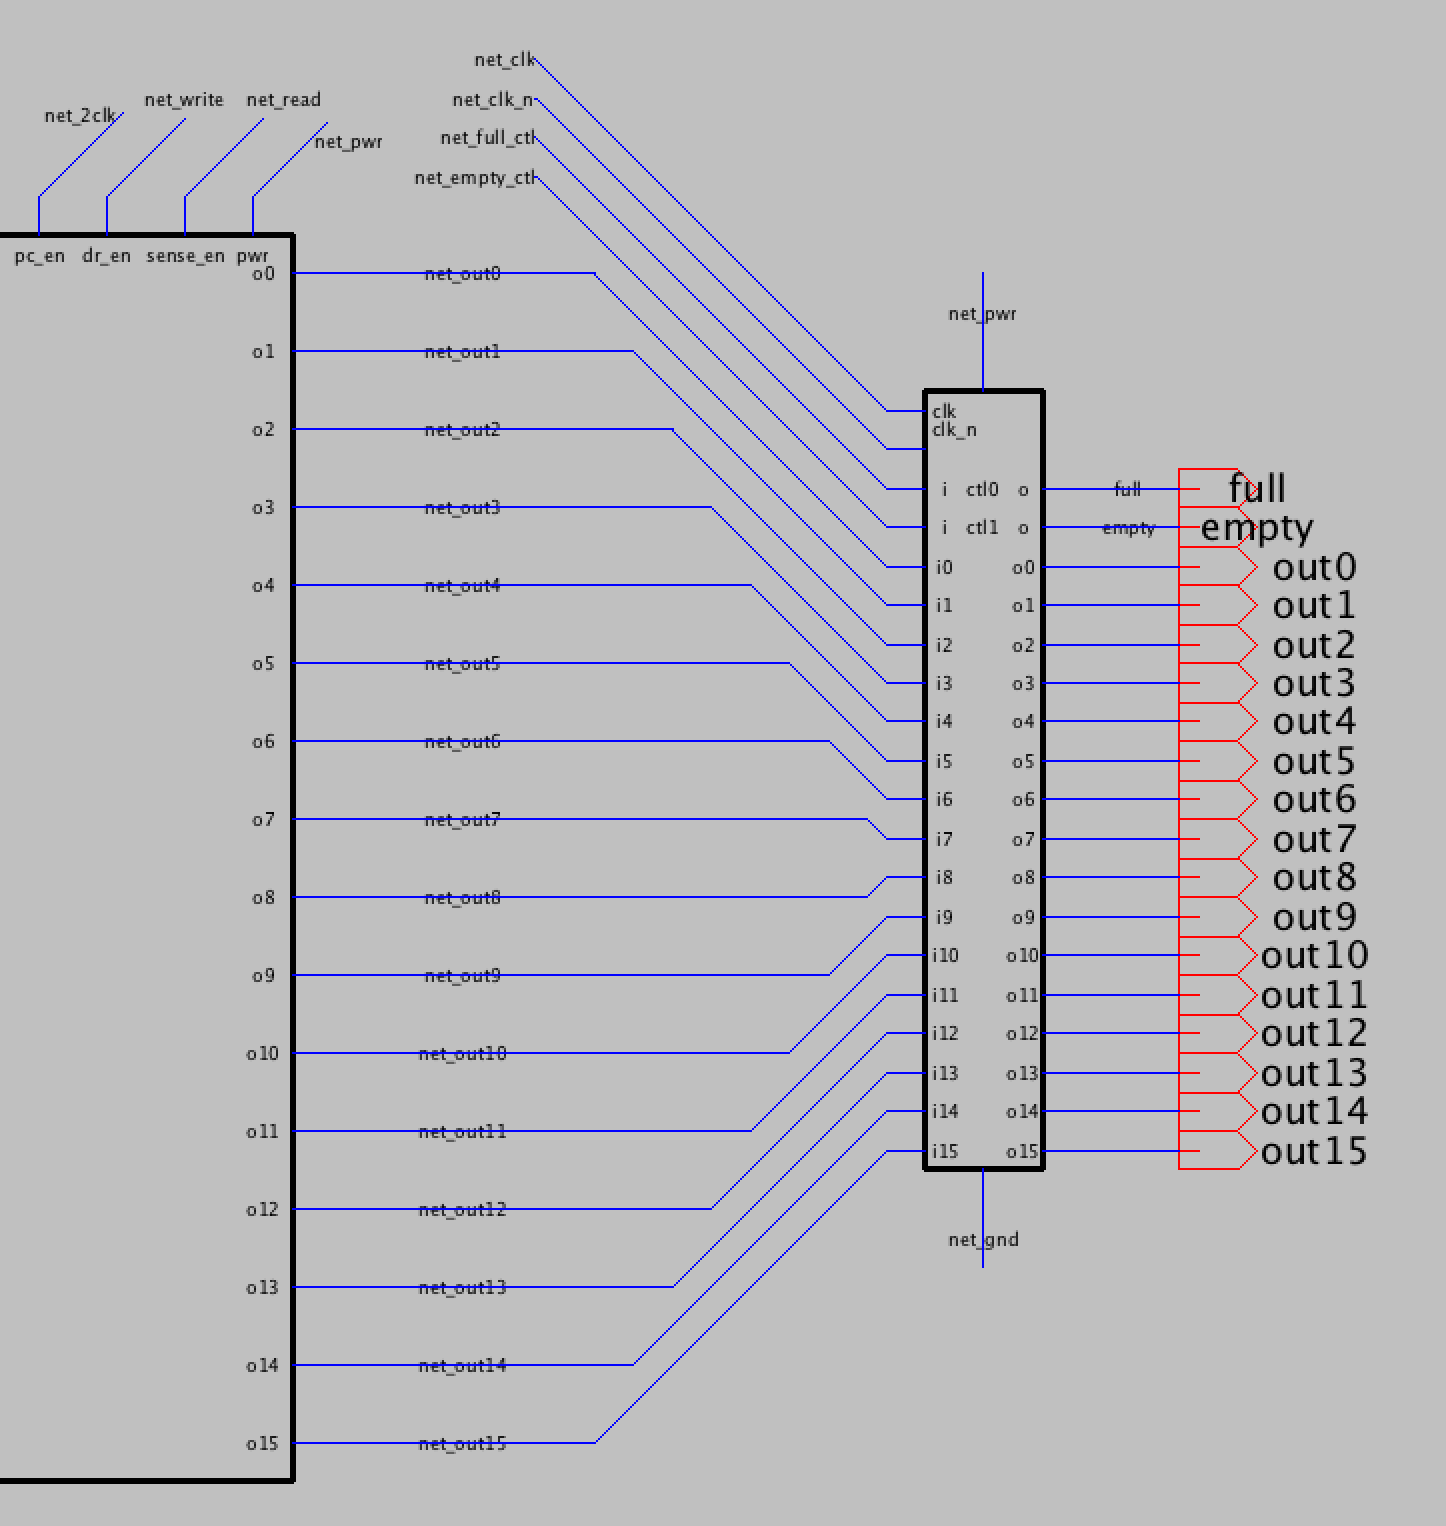
\includegraphics[scale=0.4]{topLevelSchematicRight}
	\caption{Top Level 16x16 FIFO Schematic Output}
	\label{fig:topLevelSchematicRight}
\end{figure}

\subsubsection{Validation}

We first tested a single enqueue and dequeue to test that reading and writing works, reading gives output on the correct clock cycle, and the empty singal behaves as expected. Here is the schematic:

\begin{figure}[H]
	\centering
	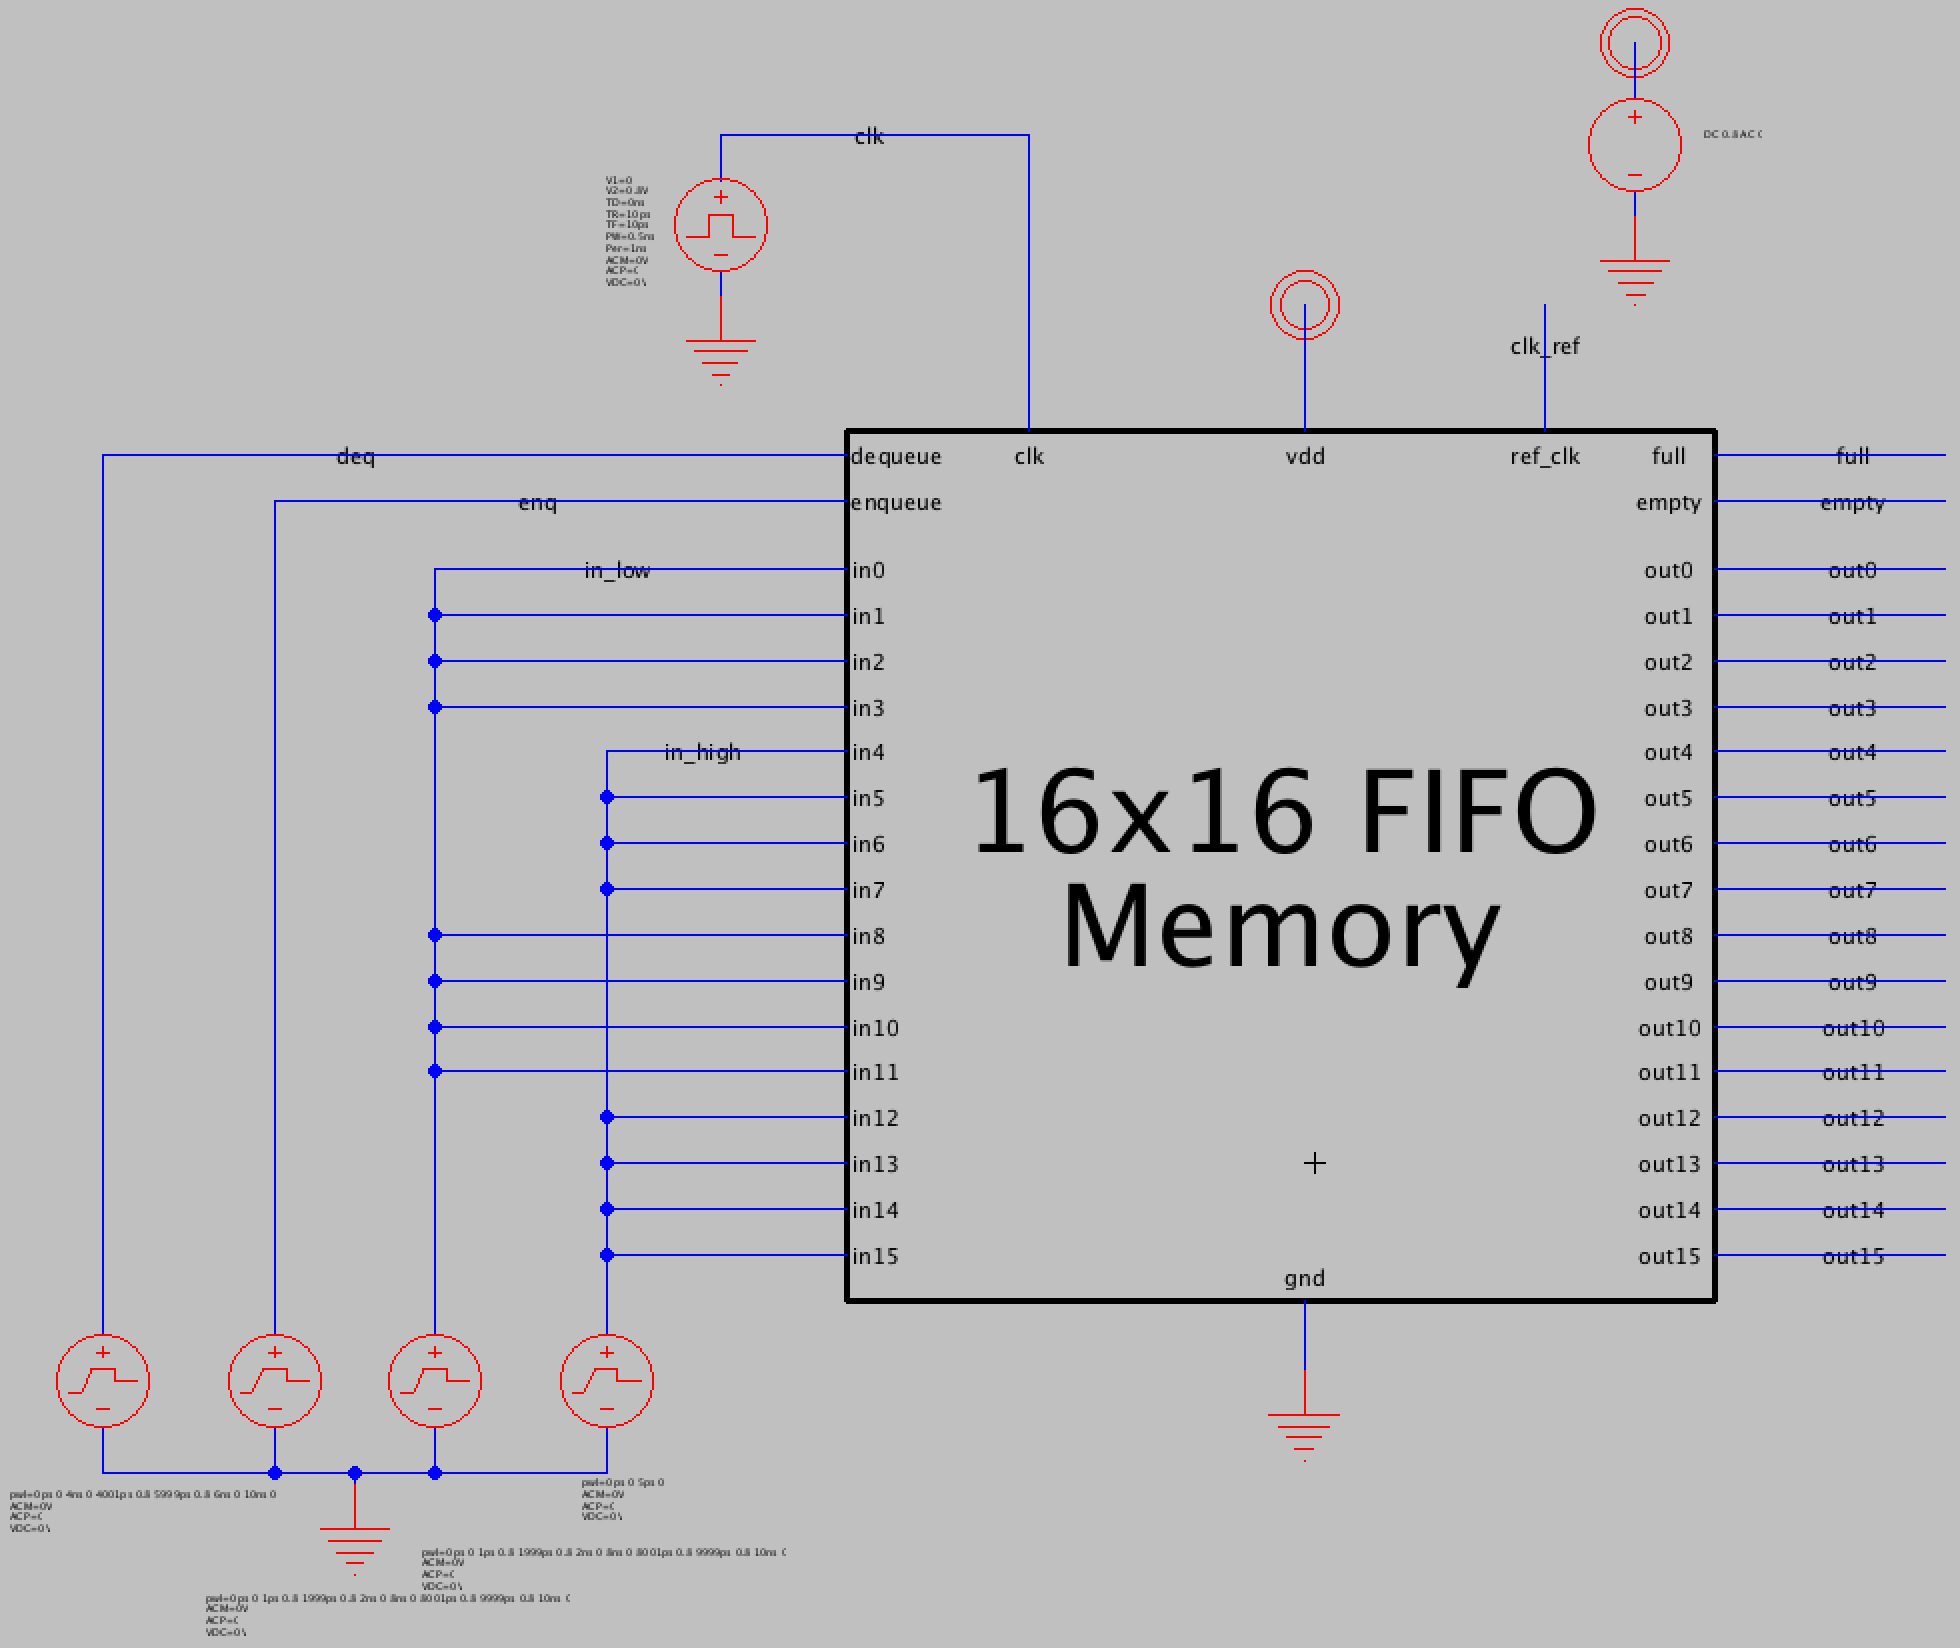
\includegraphics[scale=0.4]{topLevelTestSchematic}
	\caption{Top Level 16x16 FIFO Test Schematic}
	\label{fig:topLevelTestSchematic}
\end{figure}

The waveform in Figure \ref{fig:topLevelTestWaveform} shows the 500MHz that is generated within the FIFO memory block (which is output from the 16x16 FIFO Memory since the input is a 1GHz clock). This figure also shows the enqueue signals and dequeue signals in the second waveform, the output in the third waveform, and the empty singal in the last waveform. Notice that the empty updates on the falling edge after the FIFO Memory is enqueued, and it then rises after that data is dequeued.

\begin{figure}[H]
	\centering
	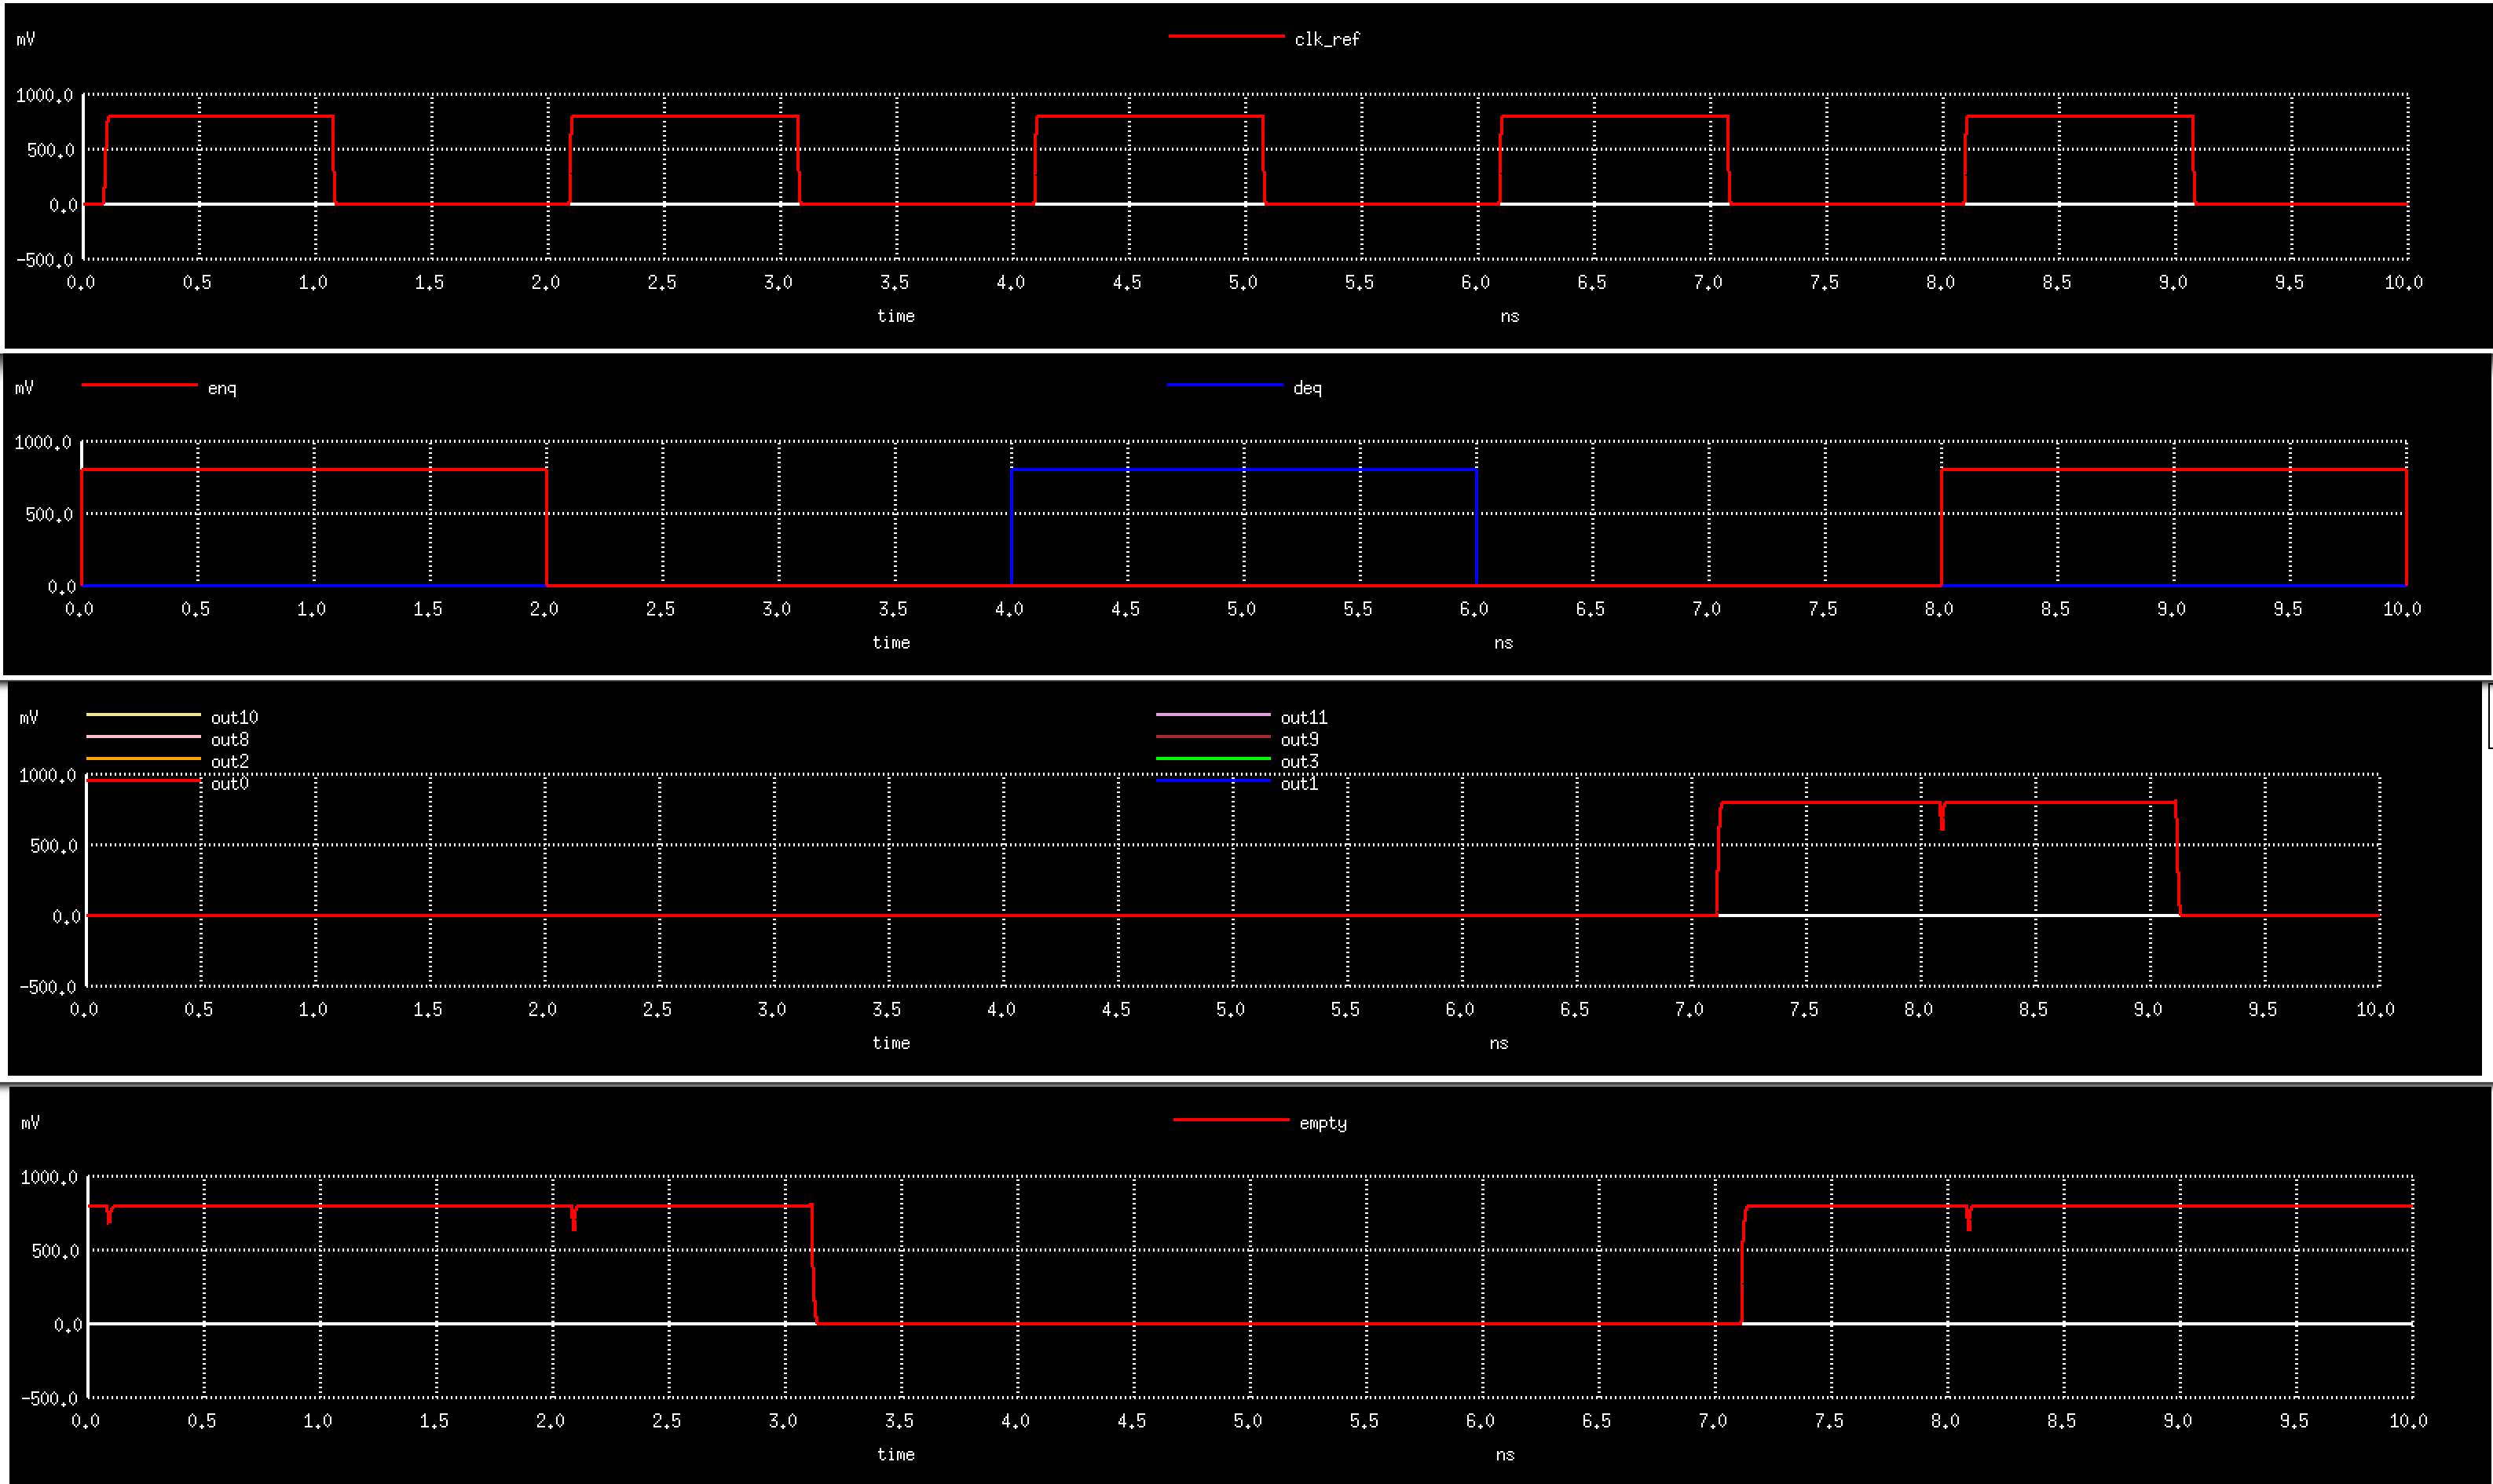
\includegraphics[scale=0.25]{topLevelTestWaveform}
	\caption{Top Level 16x16 FIFO Test Waveform}
	\label{fig:topLevelTestWaveform}
\end{figure}


\subsection{Calculations}
\label{sec:calculations}

\subsubsection{Sizing}
\label{subsec:sizing_calc}

For calculating sizing constraints, we used a 1GHz rise time for the cases of driving a 1, driving a 0, reading a 1, and reading a 0 since we need to do a read and a write in one 500GHz pulse. We estimated $\gamma = 1$. See Figure \ref{fig:sizingMath} for the output from Mathematica. The code is below:
\\\\\noindent
\code {
tau = (2.57/2.2) * 10 \textasciicircum -12 \textnormal{//$\tau$ from previous work}\\
g = 1 \textnormal{//$\gamma$ assumed to be around 1}\\
WMC = 1 \textnormal{//Width of Memory Cell Access Transistor}\\
WMCP = 1 \textnormal{//Width of Memory Cell PMOS}\\
WMCN = 1 \textnormal{//Width of Memory Cell NMOS}\\
Clear[WDP, WDN, WDE, WSA, WMC, WMCN, WMCP]\\
WDN = WDP \textnormal{//Width of Driver NMOS = Width of Driver PMOS}\\
WDP = 16 \textnormal{//Width of Driver PMOS = 16}\\
\\
\textnormal{//For the capacitance of the bitline:}\\
CBL = 16*g+g*WDE+16*g*WMC+WSA\\
\\
\textnormal{//For the Pre-Charge Rise Time}\\
PCharge = (1/16)*3*16*g*tau + (2/16)*CBL*tau\\
\\
\textnormal{//For the Drive 1 Rise Time}\\
Drive1 = (1/WDP)*g*(WDP+WDN+WDE)*tau+((1/WDP)+\\
\tab (1/WDE))*CBL*tau+((1/WDP)+(1/WDE)+(1/WMC))*2*g*tau\\
\\
\textnormal{//For the Drive 0 Fall Time}\\
Drive0 = (1/WDN)*g*(WDP+WDN+WDE)*tau+((1/WDP)+\\
\tab (1/WDE))*CBL*tau+((1/WDP)+(1/WDE)+(1/WMC))*2*g*tau\\
\\
\textnormal{//For the Read 1 Rise Time}\\
Read1 = (1/WMCP)*g*(WMCP+WMCN+WMC)*tau+((1/WMCP)+\\
\tab (1/WMC)) * CBL * tau\\
\\
\textnormal{//For the Read 0 Fall Time}\\
Read0 = (1/WMCN) * g * (WMCP + WMCN  + WMC) * tau + ((1/WMCP) +\\
\tab (1/WMC)) * CBL * tau\\
\\
\textnormal{//Find an instance where the rise and fall times are all at least 500ps and where the widths are all greater than 1}\\
FindInstance[\{2.2*PCharge, 2.2* Drive1, 2.2* Drive0, 2.2*Read1, 2.2*Read0,\\
\tab 1, 1, 1, 1, 1, 1\} <= \{500*10\textasciicircum -12, 500 10 \textasciicircum -12, 500 10\textasciicircum -12,\\
\tab 500 10\textasciicircum -12, 0.5 * 10 \textasciicircum -9, WDE, WDP, WSA, WMC, WMCN, WMCP\},\\
\tab \{WDE, WSA, WMC, WMCN, WMCP\}]\\
\textnormal{//Output}\\
\{\{WDE -> 1., WSA -> 1., WMC -> 2, WMCN -> 2, WMCP -> 2\}\}
}

\begin{figure}[H]
	\centering
	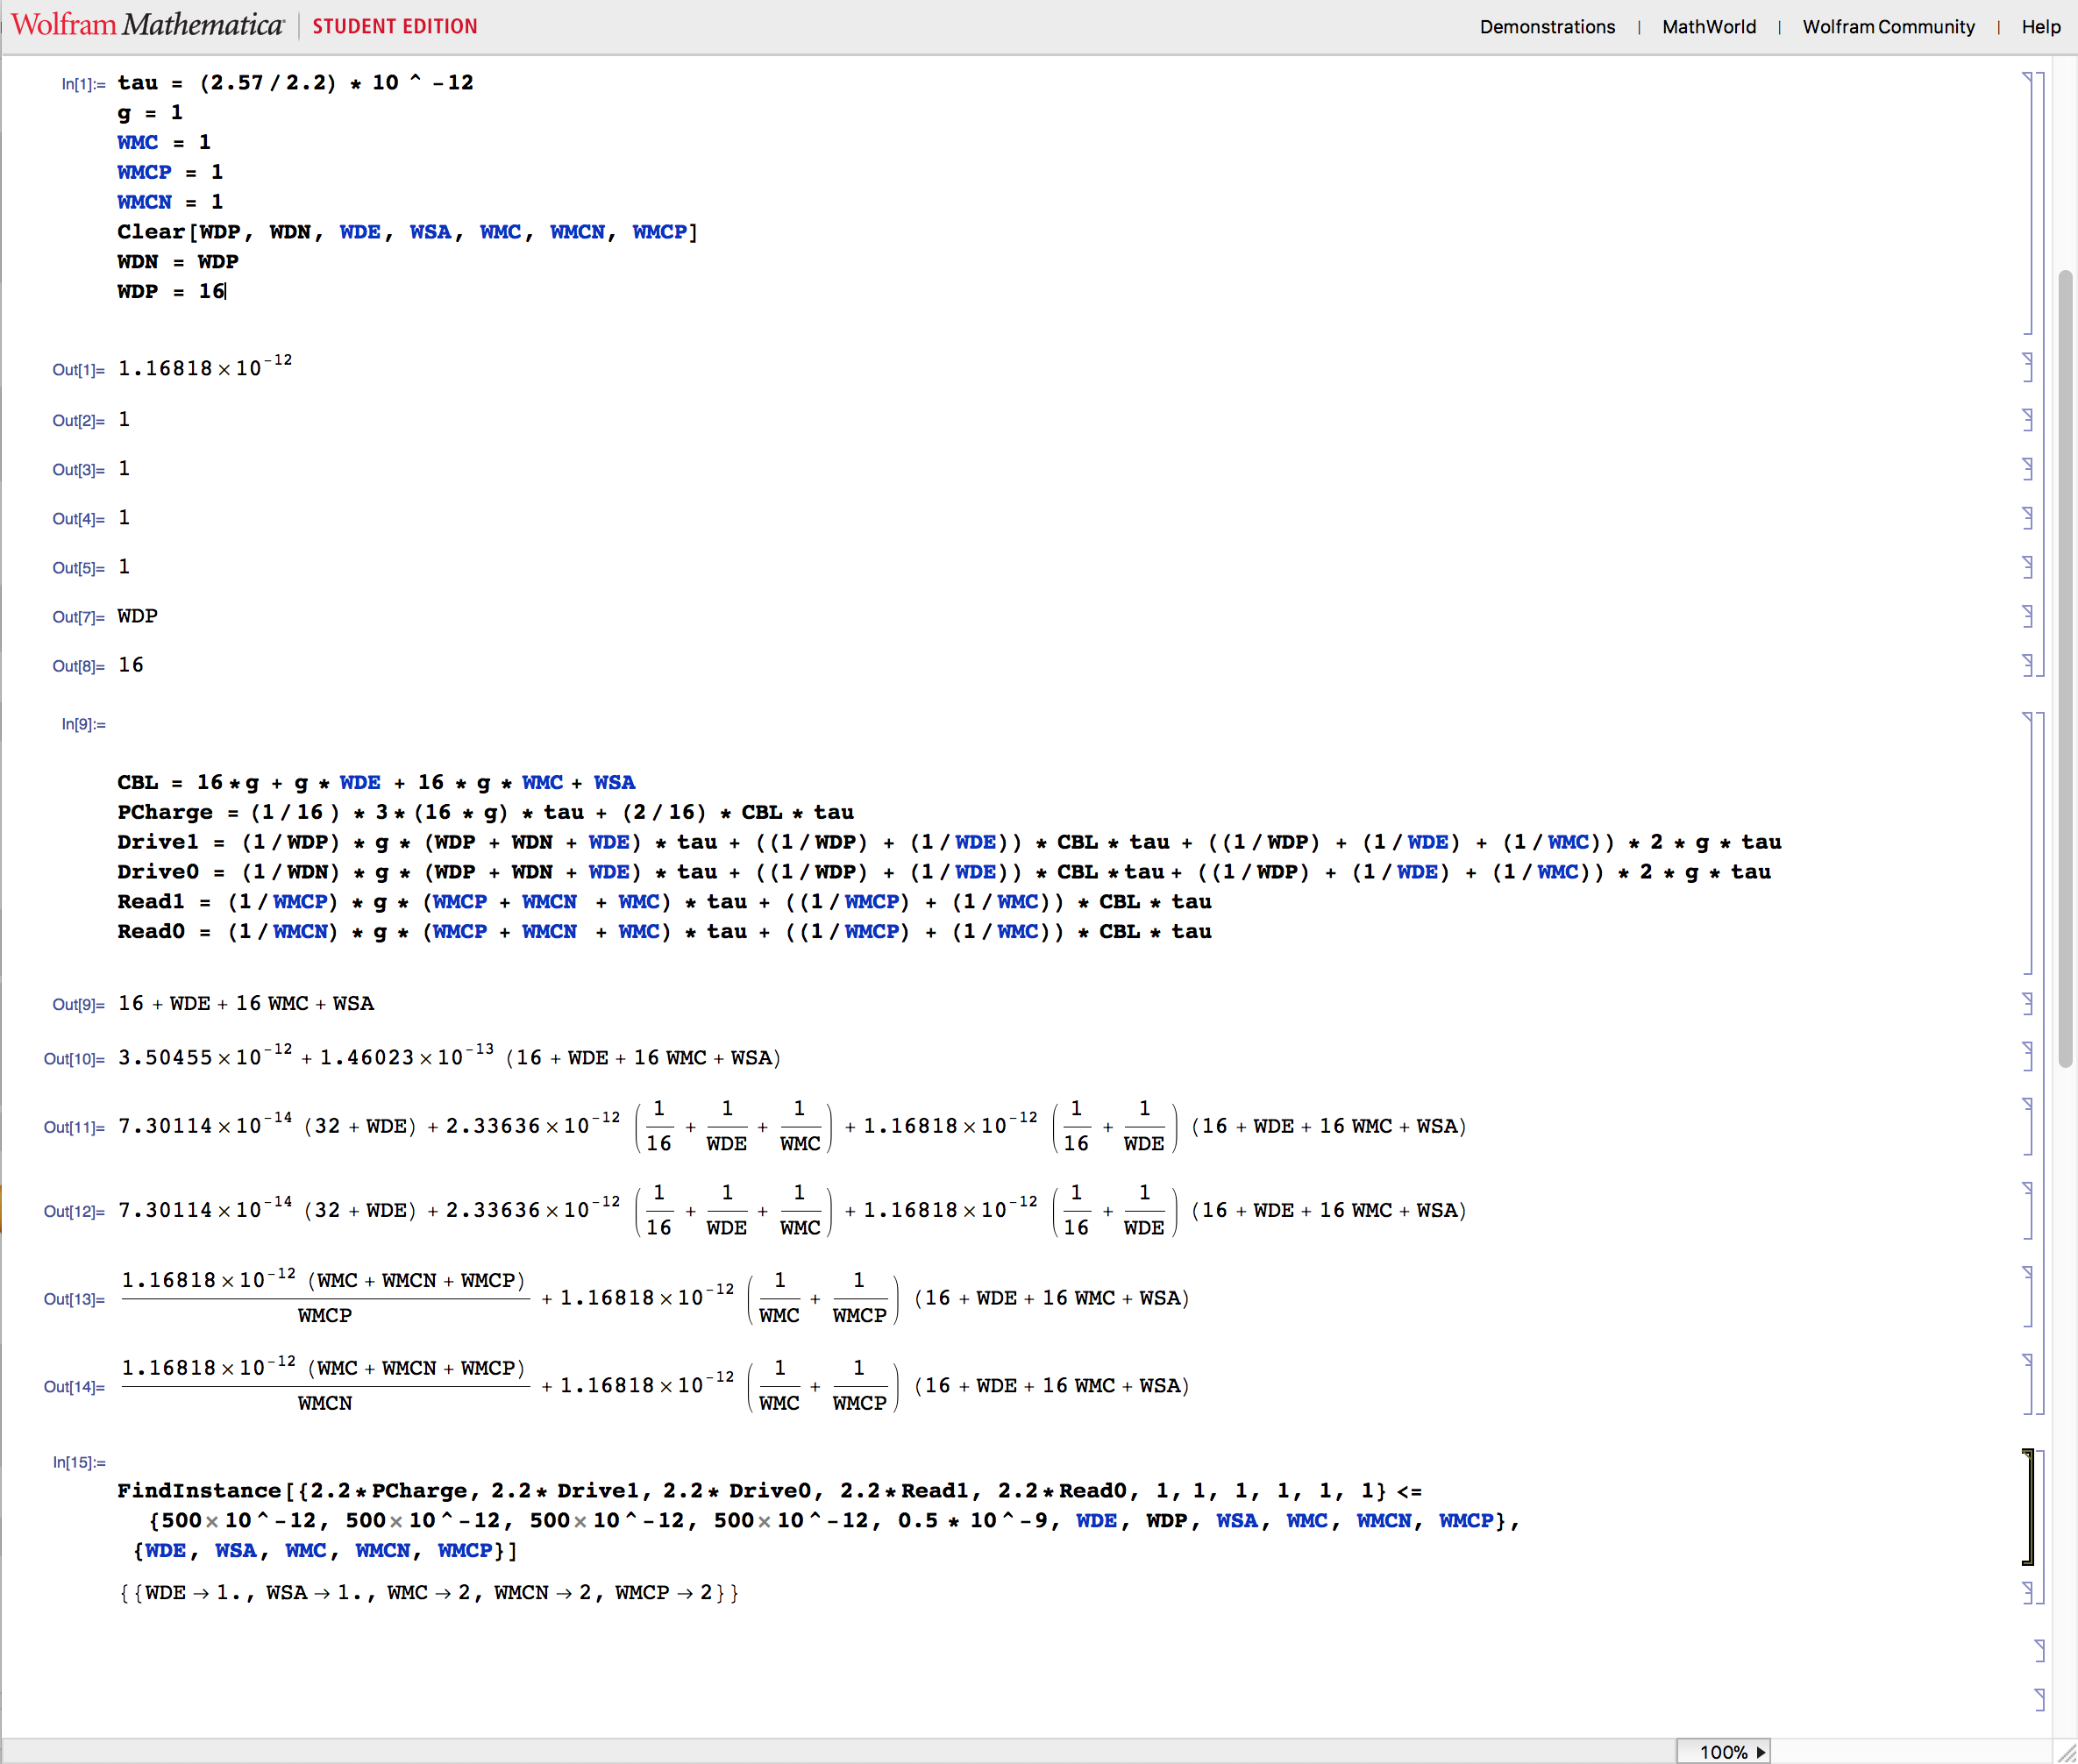
\includegraphics[scale=0.3]{sizingMath}
	\caption{Mathematica output for calculating transistor widths}
	\label{fig:sizingMath}
\end{figure}

Because of this, we sized the width of the memory cell's PMOS, NMOS, and enable transistors to 2 and the sense enable transistor to 1. 

\subsubsection{Capacitance}
\label{subsec:cap_calc}

Bitline with drive and pre-charge enable transistors off:
\begin{align*}
C_{BLtotal} &= C_{pre-charger} + C_{driver} + 16 C_{memcell} + C_{senseamp}\\
&= 16 \gamma C_0 + W_{DriveEn}\gamma C_0 + 16 W_{RWEnable}\gamma C_0 + W_{SenseAmpIn} C_0\\
&= ((16 + W_{DriveEn}  + 16 W_{RWEnable})\gamma + W_{SenseAmpIn})C_0\\\\
W_{DriveEn} &= 16\\
W_{RWEnable} &= 2\\
W_{SenseAmpIn} &= 1\\\\
C_{BLtotal} &= ((16 + 16  + 16 \times 2)\gamma + 1)C_0\\
&= ((16 + 16  + 16 \times 2)\gamma + 1)C_0\\
&= (64\gamma + 1) C_0
\end{align*}

\subsubsection{Timing}
\label{subsec:time_calc}
The calculations above for sizing were constrained by 1GHz operation. Because the rise of the bit line does not necessarily need to be the entire $2.2\tau$ (since we are only rising from $\frac{Vdd}{2} \rightarrow Vdd$ or from $\frac{Vdd}{2} \rightarrow 0$), this should leave us with widths that are greater than those actually required.


% \subsubsection{Energy}
% \begin{align*}
% E &= CV^2\\
% &= (64\gamma + 1) C_0 * Vdd^2\\
% &= (64\gamma + 1) C_0 * (0.8)^2\\
% \end{align*}

\section{Metrics}
\label{sec:metrics}

\subsection{Area}
\begin{enumerate}
\item memory cell area: 8
\item total area: $16 \times 8 + 84 + 56 + 56 + 6 = 330$
\subitem Driver = 84
\subitem Vref Generator = 56
\subitem Output Buffers = 6
\end{enumerate}

\subsection{Timing}
For timing, we constrained the sizing equations in Section \ref{subsec:sizing_calc} by a 1GHz operation (within 500ps rise time). This is so when we run the entire design at 500MHz, we can enqueue and dequeue in a single 500MHz clock cycle. We used the example bitline schematics above to find the delay from driving the wordline to the output. The delay from the drive of the wordline to the output is 133.111ps (Figure \ref{fig:ioTiming}), which gives ample room to increase as we optimize for energy.

\begin{figure}[H]
	\centering
	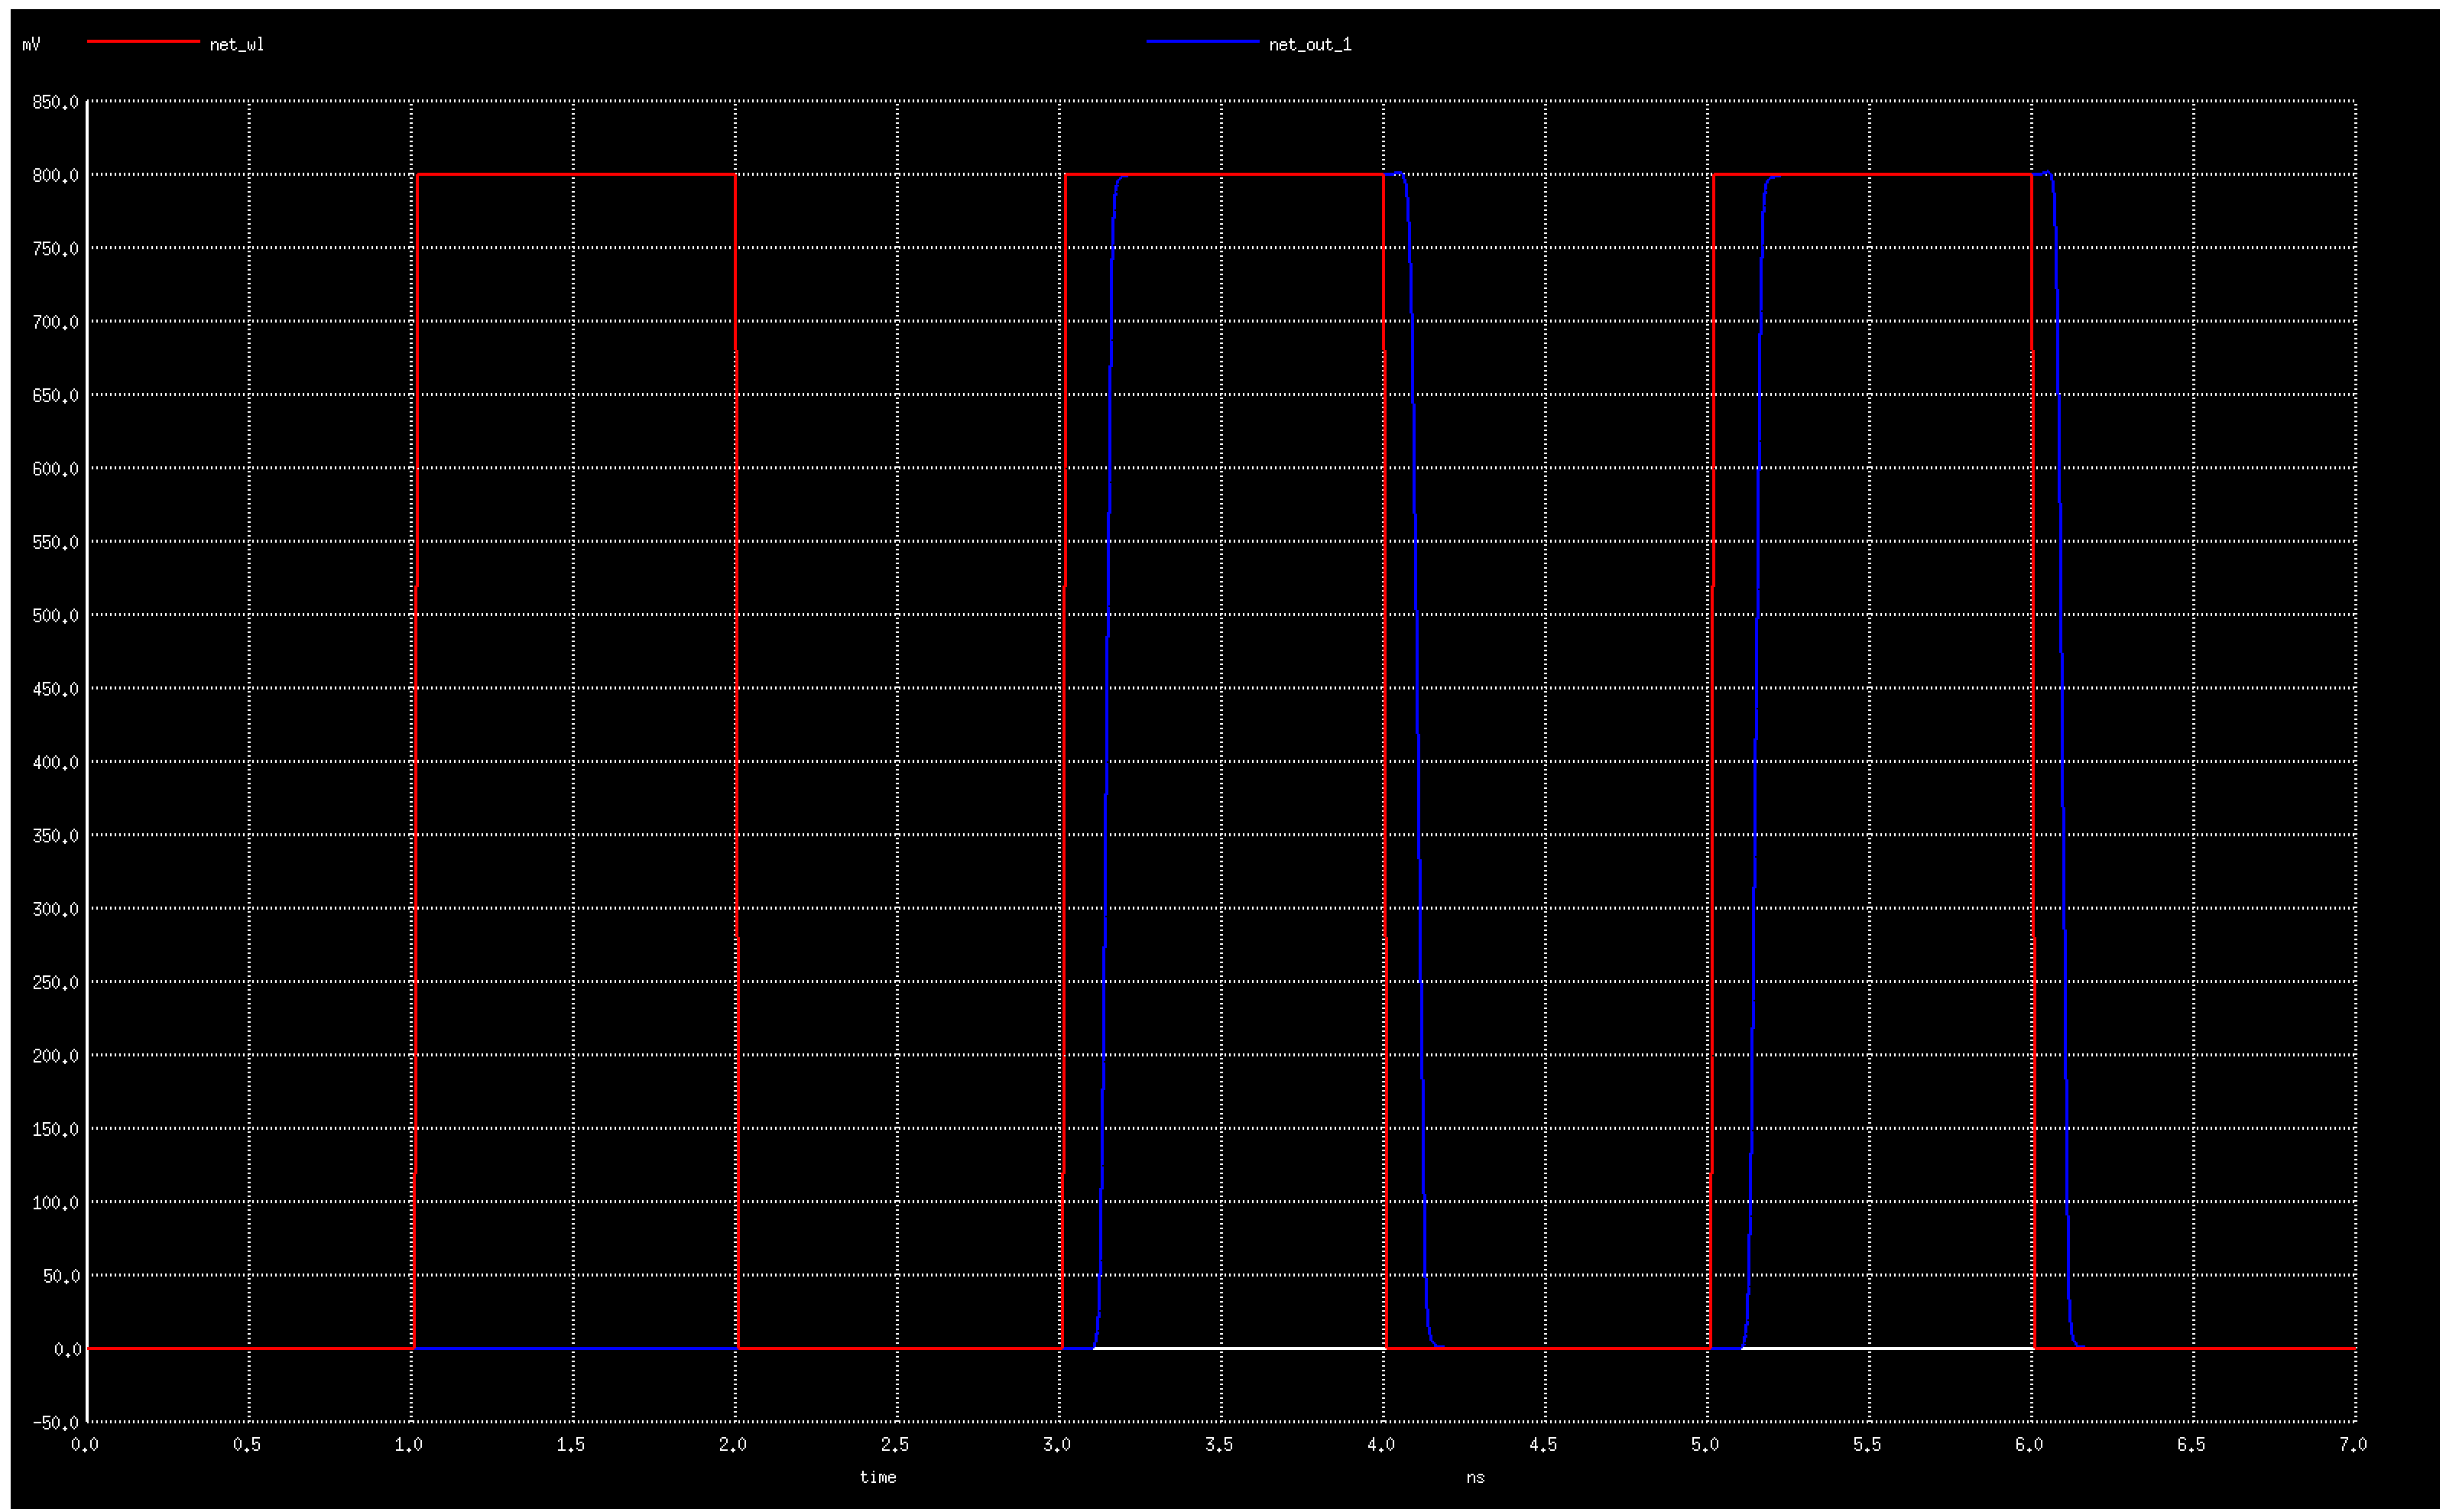
\includegraphics[scale=0.2]{exampleBitlineIOTiming}
	\caption{Wordline with Output}
	\label{fig:ioTiming}
\end{figure}



\subsection{Energy}
\subsubsection{Enqueue Energy}
To test enqueue energy, we looked at both the energy to transition from $0x0000$ to $0xFFFF$ and vice-versa. The reported values are below with the test schematic shown in Figure \ref{fig: todo} and the resulting waveforms in Figure \ref{fig: todo} and Figure \ref{fig: todo} respectively.
$$0x0000 \rightarrow 0xFFFF = xW$$
$$0xFFFF \rightarrow 0x0000 = yW$$
\subsubsection{Dequeue Energy}
This was a test for dequeueing a single value. We tested both $0x0000$ and $0xFFFF$
$$0x0000 = xW\textnormal{ (shown in Figure \ref{fig: todo})}$$
$$0xFFFF = yW\textnormal{ (shown in Figure \ref{fig: todo})}$$

\subsubsection{Enqueue/Dequeue Energy}
The energy for a single enqueue and dequeue is as follows:

% \newpage
% \section{Some LaTeX tips}
% \label{sec:latex}
% \subsection{How to Include Figures}

% First you have to upload the image file (JPEG, PNG or PDF) from your computer to writeLaTeX using the upload link the project menu. Then use the includegraphics command to include it in your document. Use the figure environment and the caption command to add a number and a caption to your figure. See the code for Figure \ref{fig:frog} in this section for an example.

% % \begin{figure}
% % \centering
% % \includegraphics[width=0.3\textwidth]{frog.jpg}
% % \caption{\label{fig:frog}This frog was uploaded to writeLaTeX via the project menu.}
% % \end{figure}

% \subsection{How to Make Tables}

% Use the table and tabular commands for basic tables --- see Table~\ref{tab:widgets}, for example.

% \begin{table}
% \centering
% \begin{tabular}{l|r}
% Item & Quantity \\\hline
% Widgets & 42 \\
% Gadgets & 13
% \end{tabular}
% \caption{\label{tab:widgets}An example table.}
% \end{table}

% \subsection{How to Write Mathematics}

% \LaTeX{} is great at typesetting mathematics. Let $X_1, X_2, \ldots, X_n$ be a sequence of independent and identically distributed random variables with $\text{E}[X_i] = \mu$ and $\text{Var}[X_i] = \sigma^2 < \infty$, and let

% \begin{equation}
% S_n = \frac{X_1 + X_2 + \cdots + X_n}{n}
%       = \frac{1}{n}\sum_{i}^{n} X_i
% \label{eq:sn}
% \end{equation}

% denote their mean. Then as $n$ approaches infinity, the random variables $\sqrt{n}(S_n - \mu)$ converge in distribution to a normal $\mathcal{N}(0, \sigma^2)$.

% The equation \ref{eq:sn} is very nice.

% \subsection{How to Make Sections and Subsections}

% Use section and subsection commands to organize your document. \LaTeX{} handles all the formatting and numbering automatically. Use ref and label commands for cross-references.

% \subsection{How to Make Lists}

% You can make lists with automatic numbering \dots

% \begin{enumerate}
% \item Like this,
% \item and like this.
% \end{enumerate}
% \dots or bullet points \dots
% \begin{itemize}
% \item Like this,
% \item and like this.
% \end{itemize}
% \dots or with words and descriptions \dots
% \begin{description}
% \item[Word] Definition
% \item[Concept] Explanation
% \item[Idea] Text
% \end{description}

% We hope you find write\LaTeX\ useful, and please let us know if you have any feedback using the help menu above.

\section{Code of Academic Integrity}
I, Phillip Trent, certify that I have complied with the University of Pennsylvania’s Code of Academic Integrity in completing this project.\\
I, Dane Walton, certify that I have complied with the University of Pennsylvania’s Code of Academic Integrity in completing this project.
\end{document}



